% Tipe dokumen adalah report dengan satu kolom kertas A4; margin tiap halaman tetap.
% Ukuran font 12pt
\documentclass[12pt, a4paper, onecolumn, oneside, openany, final]{report}

% Load konfigurasi LaTeX untuk tipe laporan thesis
\usepackage{ta}
\counterwithin{algorithm}{chapter}
\usepackage{longtable}
\usepackage{booktabs}
\usepackage{siunitx}
\usepackage[indonesian]{babel}
\addto\captionsindonesian{
  \def\refname{Referensi}% 
  \def\contentsname{Daftar Isi}%
}

\usepackage{pdflscape}

% Margin kiri dan kanan sama pada setiap halaman. Footer diperluas sampai
% tepi kertas supaya angka tetap di tengah fisik halaman.
\newcommand{\centeredpagefooter}{%
  \fancyfoot[C]{\thepage}%
  \fancyfootoffset[L]{4cm}%
  \fancyfootoffset[R]{2.5cm}%
}

% Halaman awal memakai angka Romawi di tengah bawah.
\fancypagestyle{romanstyle}{%
  \fancyhf{}%
  \centeredpagefooter
  \renewcommand{\headrulewidth}{0pt}%
  \renewcommand{\footrulewidth}{0pt}%
}

% Halaman isi memakai angka di kanan atas pada setiap halaman.
\fancypagestyle{mainstyle}{%
  \fancyhf{}%
  \fancyfootoffset[OL,OR]{0pt}%
  \fancyhead[R]{\thepage}%
  \renewcommand{\headrulewidth}{0pt}%
  \renewcommand{\footrulewidth}{0pt}%
}

% Kelas report memakai style plain pada halaman awal bab dan daftar.
\fancypagestyle{chapterstart}{%
  \fancyhf{}%
  \centeredpagefooter
  \renewcommand{\headrulewidth}{0pt}%
  \renewcommand{\footrulewidth}{0pt}%
}
\fancypagestyle{plain}[chapterstart]{}

% Load konfigurasi khusus untuk laporan yang sedang dibuat
%-----------------------------------------------------------------------------%
% Informasi Mengenai Dokumen
% Ganti semua isian bertanda [ ... ] sebelum diserahkan.
%-----------------------------------------------------------------------------%
%
% Judul laporan (bahasa Indonesia). Istilah asing ditulis miring.
% Judul dikembangkan dari "Skripsi Arahan Pak Budi" (Laravel + Vue.js + PWA) menjadi FastAPI + Vue.js berbasis web
% dengan modul rekomendasi berbasis kecerdasan buatan, sesuai keputusan 30 September 2026.
\var{\judul}{RANCANG BANGUN APLIKASI WEB MANAJEMEN RESEP DAN STANDARDISASI OPERASIONAL KEDAI KOPI DENGAN REKOMENDASI BERBASIS KECERDASAN BUATAN MENGGUNAKAN \textit{FRAMEWORK} FASTAPI DAN VUE.JS}
\Var{\Judul}{RANCANG BANGUN APLIKASI WEB MANAJEMEN RESEP DAN STANDARDISASI OPERASIONAL KEDAI KOPI DENGAN REKOMENDASI BERBASIS KECERDASAN BUATAN MENGGUNAKAN \textit{FRAMEWORK} FASTAPI DAN VUE.JS}
\Var{\JudulIndo}{RANCANG BANGUN APLIKASI WEB MANAJEMEN RESEP DAN STANDARDISASI OPERASIONAL KEDAI KOPI DENGAN REKOMENDASI BERBASIS KECERDASAN BUATAN MENGGUNAKAN \textit{FRAMEWORK} FASTAPI DAN VUE.JS}
% Judul bahasa Inggris
\Var{\JudulInggris}{DESIGN AND DEVELOPMENT OF A WEB-BASED RECIPE MANAGEMENT AND OPERATIONAL STANDARDIZATION APPLICATION FOR COFFEE SHOPS WITH ARTIFICIAL INTELLIGENCE-BASED RECOMMENDATIONS USING FASTAPI AND VUE.JS}

% Tipe laporan
\var{\type}{Skripsi}
\Var{\Type}{SKRIPSI}

% Identitas penulis (placeholder). Untuk skripsi kelompok, tambahkan
% \penulisDua dan seterusnya lalu sesuaikan sampul.tex dan halaman pernyataan.
\var{\penulis}{[Nama Mahasiswa]}
\Var{\Penulis}{[Nama Mahasiswa]}
\var{\nim}{[NIM]}
\var{\penulisSatu}{[Nama Mahasiswa]}
\var{\NIMpenulisSatu}{[NIM]}
\var{\inisialPenulis}{[Inisial]}
\var{\email}{[email]@binus.ac.id}

% Fakultas dan program studi
\Var{\Fakultas}{School of Computer Science}
\var{\fakultas}{School of Computer Science}
\Var{\Program}{Computer Science Study Program}
\var{\program}{Computer Science Study Program}
\var{\kota}{Bandung}
\Var{\Kota}{Bandung}
\Var{\Tahun}{2026}
\var{\tahun}{2026}
% https://binus.ac.id/bandung/computer-science/ menyebut Academic Title: Sarjana Komputer (S.Kom.).
\var{\gelar}{Sarjana Komputer}
\var{\tanggalPengesahan}{\today}

% Pembimbing (placeholder)
\var{\pembimbingSatu}{[Nama Dosen Pembimbing, Gelar]}
\var{\nikSatu}{[NIK/NIDN]}

%-----------------------------------------------------------------------------%
% Judul Setiap Bab (Petunjuk Penulisan Skripsi CS BINUS Bandung, Feb 2026)
%-----------------------------------------------------------------------------%
\var{\abstrak}{Abstrak}
\Var{\kataPengantar}{Kata Pengantar}
\Var{\babSatu}{Pendahuluan}
\Var{\babDua}{Tinjauan Referensi}
\Var{\babTiga}{Metode Penelitian}
\Var{\babEmpat}{Hasil dan Pembahasan}
\Var{\babLima}{Simpulan dan Saran}


\usepackage{titlesec}
\titlespacing*{\subsection}{0.5cm}{3.5ex plus 1ex minus .2ex}{2.3ex plus .2ex}
\titlespacing*{\subsubsection}{1.0cm}{3.25ex plus 1ex minus .2ex}{1.5ex plus .2ex}
\usepackage{titletoc}
\titlecontents{chapter}[0em]
  {\addvspace{1em}\bfseries}
  {BAB \thecontentslabel\quad}
  {}
  {\hfill\contentspage}
% Awal bagian penulisan laporan
% Sitasi APA berbahasa Indonesia. Aturan BINUS: "et al." hanya untuk >5 penulis,
% jadi sumber 1-5 penulis disitasi dengan \citet*{} / \citep*{} (daftar penulis lengkap).
\AtBeginDocument{%
  \renewcommand{\BBAB}{dan}%
  % "et al." muncul hanya untuk sumber >5 penulis (aturan BINUS); dalam bahasa
  % Indonesia ditulis "dkk.". Daftar referensi tetap memakai "&" sesuai contoh panduan.
  \renewcommand{\BOthers}[1]{dkk.\hbox{}}%
  \renewcommand{\BOthersPeriod}[1]{dkk.\hbox{}}%
  \renewcommand{\BRetrievedFrom}{Diakses dari\ }%
  \renewcommand{\BRetrieved}[1]{Diakses #1, dari\ }}
\begin{document}

% Sampul Laporan
\begin{titlepage}
    \begin{center}
        % Judul dan jenis karya (Times New Roman, tebal)
        \bo{\large{\JudulIndo}} \\[0.75cm]

        \vspace*{0.7 cm}
        \bo{\large{\Type}}  \\
        \vspace*{0.8 cm}

        \bo{oleh}\\
        \bo{\large{\penulisSatu}} \quad \bo{\large{\NIMpenulisSatu}} \\

        \vspace*{0.7 cm}
        \begin{figure}[H]
            \centering
            
\includegraphics[width=0.7\linewidth]{pic/logo.png}
        \end{figure}

        \bo{\doublespacing
            \large{\program}\\
            \large{\fakultas} \\
            \large{Universitas Bina Nusantara}\\
            \large{\Kota} \\
            \large{\tahun}
        }
    \end{center}
\end{titlepage}


%comment dari sini%

\pagenumbering{gobble}

% Halaman pengesahan
% \addChapter{LEMBAR PENGESAHAN}
% \thispagestyle{plain}
\begin{center}
        \bo{{\JudulIndo}} \\[0.75cm]
        \bo{SKRIPSI}

        \vspace*{0.1 cm}
        \bo{Disusun oleh}\\
        \vspace{2.2cm}% ruang tanda tangan
        \underline{\makebox[6cm][c]{\penulisSatu}}\\[4pt]
        \fontsize{12}{14}\selectfont\bf{\NIMpenulisSatu}

        \vspace*{0.9 cm}
        \bo{Disetujui oleh}:\\
        \bo{Pembimbing dan Head of Study Program}\\
\end{center}

    \vspace{1.2cm}
    \begin{center}
    \begin{minipage}{12cm}
        \centering
        \vspace*{1.8cm}% ruang tanda tangan
        \underline{\pembimbingSatu} \\[4pt]
        \fontsize{12}{14}\selectfont\bf{\nikSatu}\\
    \end{minipage}
    \end{center}


%comment disini%

% Gunakan penomoran halaman romawi
\pagenumbering{roman}
\pagestyle{romanstyle}
% setelah bagian ini, halaman dihitung sebagai halaman ke 2
\setcounter{page}{2}

%comment sini%

% Sampul ke dua
\thispagestyle{plain}
    \begin{center}
        \bo{\large{\JudulIndo}} \\[0.75cm]

        \vspace*{0.7 cm}
        \bo{\large{\Type}}  \\
        \vspace*{0.1 cm}
        \textbf{diajukan sebagai salah satu syarat} \\
        \textbf{untuk gelar kesarjanaan pada} \\
        \textbf{Program Studi Teknik Informatika} \\
        \textbf{Jenjang Pendidikan Strata-1} \\
        \vspace*{0.5cm}

        \bo{oleh}\\
        \bo{\large{\penulisSatu}} \quad \bo{\large{\NIMpenulisSatu}} \\

        \begin{figure}[H]
            \centering
            
\includegraphics[width=0.5\linewidth]{pic/logo.png}
        \end{figure}

        \bo{\doublespacing
            \large{\program}\\
            \large{\fakultas} \\
            \large{Universitas Bina Nusantara}\\
            \large{\Kota} \\
            \large{\tahun}
        }
    \end{center}


% Halaman pernyataan orisinalitas
% \addChapter{LEMBAR PERNYATAAN ORISINALITAS}
\thispagestyle{plain}
    \begin{center}
    \textbf{Universitas Bina Nusantara}\\
    \vspace*{-0.5cm}
    \rule{13cm}{1pt} \\
    \vspace*{-0.2cm}
    \textbf{Pernyataan Kesiapan Skripsi untuk Ujian Pendadaran}
    \end{center}

    \textbf{Pernyataan Penyusunan Skripsi}\\
    \indent\textbf{Saya},

    \indent\textbf{\penulisSatu},

    \textbf{dengan ini menyatakan bahwa Skripsi yang berjudul}:

    \begin{center}
    \textbf{\Judul}\\
    \textit{\textbf{\JudulInggris}}\\
    \end{center}

    \noindent\textbf{adalah benar hasil karya saya dan belum pernah diajukan sebagai karya ilmiah, sebagian atau seluruhnya, atas nama saya atau pihak lain.}

    \vspace{1.5cm}
    \begin{center}
        \begin{minipage}{8cm}
        \centering
        \vspace*{1.8cm}% ruang tanda tangan
        \underline{\makebox[6cm][c]{\penulisSatu}}\\[4pt]
        \fontsize{12}{14}\selectfont\bf{\NIMpenulisSatu}
        \end{minipage}
    \end{center}

    \begin{center}
    \textbf{Disetujui oleh Pembimbing}\\
    \textbf{Saya setuju Skripsi tersebut layak diajukan untuk Ujian Pendadaran} \\
    \end{center}

    \vspace{0.5cm}
    \begin{center}
        \begin{minipage}{10cm}
        \centering
        \vspace*{1.8cm}% ruang tanda tangan
        \underline{\pembimbingSatu}\\[4pt]
        \fontsize{12}{14}\selectfont\bf{\nikSatu}\\
        \end{minipage}
    \end{center}
    \begin{center}
        \Kota, \tanggalPengesahan \\
    \end{center}


% PENGESAHAN
\thispagestyle{plain}
\begin{center}
        \bo{{\JudulIndo}} \\[0.75cm]
        \bo{SKRIPSI}

        \vspace*{0.1 cm}
        \bo{Disusun oleh}\\
        \vspace{2.2cm}% ruang tanda tangan
        \underline{\makebox[6cm][c]{\penulisSatu}}\\[4pt]
        \fontsize{12}{14}\selectfont\bf{\NIMpenulisSatu}

        \vspace*{0.9 cm}
        \bo{Disetujui oleh}:\\
        \bo{Pembimbing dan Head of Study Program}\\
\end{center}

    \vspace{1.2cm}
    \begin{center}
    \begin{minipage}{12cm}
        \centering
        \vspace*{1.8cm}% ruang tanda tangan
        \underline{\pembimbingSatu} \\[4pt]
        \fontsize{12}{14}\selectfont\bf{\nikSatu}\\
    \end{minipage}
    \end{center}


% PERNYATAAN
\thispagestyle{plain}
\centering{\large{\bo{PERNYATAAN}}}
\vspace*{.3cm}

\justifying
\noindent Dengan ini saya, \\

\noindent
\begin{tabular}{l c p{0.65\textwidth}}
Nama          & : & \penulisSatu \\
Judul Skripsi & : & \Judul \\
\end{tabular}

\vspace*{0.5cm}
Memberikan kepada Universitas Bina Nusantara hak non-eksklusif untuk menyimpan, memperbanyak, dan menyebarluaskan Skripsi karya saya, secara keseluruhan atau hanya sebagian atau hanya ringkasannya saja, dalam bentuk format tercetak dan atau elektronik.

Menyatakan bahwa saya akan mempertahankan \textbf{hak eksklusif} saya untuk menggunakan seluruh atau sebagian isi Skripsi saya guna pengembangan karya di masa depan, misalnya dalam bentuk artikel, buku, perangkat lunak, ataupun sistem informasi.

\vspace*{0.5cm}
\noindent \Kota, \tanggalPengesahan,\\[0.3cm]
\begin{center}
\begin{minipage}{8cm}
\centering
\vspace*{1.8cm}% ruang tanda tangan
\underline{\makebox[6cm][c]{\penulisSatu}}\\[4pt]
\fontsize{12}{14}\selectfont\bf{\NIMpenulisSatu}
\end{minipage}
\end{center}

\vspace*{0.5cm}
\begin{center}
Diketahui oleh,\\[0.8cm]
\begin{minipage}{10cm}
\centering
\vspace*{1.8cm}% ruang tanda tangan
\underline{{\pembimbingSatu}}\\[4pt]
\fontsize{12}{14}\selectfont\bf{\nikSatu}\\
\end{minipage}
\end{center}


% Abstrak Bahasa Indonesia dan Bahasa Iggris
% \addChapter{ABSTRAK}
\addcontentsline{toc}{section}{Abstract}
\thispagestyle{plain}

% Angka H1--H4: results/scaling_eval.json dan results/external/E1--E3*.json.
% H5: results/assistant_eval.json (penilai versi 2.1); uji regresi internal.
\edef\abstrakRightHyphenMin{\the\righthyphenmin}
\righthyphenmin=3
\hyphenation{FastAPI Vue-js FP-Growth ber-ba-sis re-ko-men-da-si pen-ska-la-an per-se-di-a-an}

\begin{singlespace}
{\centering
    \textbf{UNIVERSITAS BINA NUSANTARA}\par
    \vspace{0.18 cm}
    Computer Science Study Program\par
    School of Computer Science\par
    Skripsi Sarjana Komputer\par
    \vspace{0.2 cm}
    \bo{\JudulIndo}\par
    \vspace{0.1 cm}
    \penulisSatu\ - \NIMpenulisSatu\par
}

{\centering\fontsize{16}{19}\selectfont\textbf{ABSTRACT}\par}

\vspace{0.08 cm}

{\centering\itshape\JudulInggris\par}

\vspace{0.1 cm}

{\itshape
\noindent Coffee shops need consistent recipes, yet orders and stock are often calculated separately. Takar is a FastAPI and Vue.js application for recipes, SOPs, constraint-aware scaling, inventory, AI decisions, and a local retrieval-and-tool assistant. Fictitious samples guided development; real data supplied external checks; 60 internal questions assessed the assistant. In 525 orders, scaling yielded no fractional shots, cup overflow above 5\%, or ratio deviation above 0.2; raw linear scaling yielded 240 fractional shots and 267 overflows. FP-Growth did not reliably beat popularity on real Bread Basket data, nor did the selected forecaster beat seasonal naive on real ihelon drinks. Simulated forecast-based restocking reached a 0.9605 fill rate versus 0.7900 for static reorder points. After benchmark-guided routing, the full assistant scored 95.0\% versus 15.0\% closed-book, with 0\% versus 85.98\% unsupported numbers. Automated tests passed; user acceptance remains unmeasured. (\inisialPenulis)

\vspace{0.2\baselineskip}

\noindent\textbf{Keywords}: standardized recipe, recipe scaling, recommender system, demand forecasting, coffee shop
}

\clearpage
\thispagestyle{plain}
\phantomsection
\addcontentsline{toc}{section}{Abstrak}

{\centering\fontsize{16}{19}\selectfont\textbf{ABSTRAK}\par}

\vspace{0.1 cm}

\noindent Kedai kopi memerlukan resep konsisten, tetapi pesanan dan stok kerap dihitung terpisah. Takar adalah aplikasi FastAPI dan Vue.js untuk resep, SOP, penskalaan berbasis batasan, inventaris, keputusan AI, dan asisten lokal dengan pencarian serta alat. Data sampel fiktif mendukung pengembangan; data nyata dipakai sebagai pemeriksaan eksternal; 60 pertanyaan internal menilai asisten. Pada 525 pesanan, penskalaan tidak menghasilkan \textit{shot} pecahan, luapan di atas 5\%, atau penyimpangan rasio di atas 0,2; penskalaan linier mentah menghasilkan 240 \textit{shot} pecahan dan 267 luapan. FP-Growth tidak mengungguli popularitas secara meyakinkan pada Bread Basket nyata, begitu pula peramal terpilih terhadap \textit{seasonal naive} pada minuman ihelon nyata. Simulasi pemesanan ulang berbasis prakiraan mencapai \textit{fill rate} 0,9605 berbanding 0,7900 untuk titik pesan ulang statis. Setelah router diperbaiki memakai tolok ukur internal, akurasi asisten lengkap 95,0\% berbanding 15,0\% tanpa konteks, dengan angka tanpa dasar 0\% berbanding 85,98\%. Pengujian otomatis lulus; UAT belum dilakukan. (\inisialPenulis)

\vspace{0.2\baselineskip}

\noindent\textbf{Kata Kunci}: resep standar, penskalaan resep, sistem rekomendasi, peramalan permintaan, kedai kopi
\end{singlespace}

% Kembalikan nilai \righthyphenmin untuk bagian berikutnya.
\righthyphenmin=\abstrakRightHyphenMin\relax


% Kata Pengantar
% \addChapter{\kataPengantar}
% \addcontentsline{toc}{section}{Kata Pengantar}
\addcontentsline{toc}{section}{Kata Pengantar}
\thispagestyle{plain}
\section*{\centering{\large{KATA PENGANTAR}}}
\justifying
\setstretch{1.5}
% Pejabat per 1 Oktober 2026: https://qmc.binus.ac.id/2026/08/25/rapat-tinjauan-manajemen-2026/
% dan https://binus.ac.id/bandung/computer-science/ (bagian PEOPLE).
Puji syukur kepada Tuhan Yang Maha Esa atas selesainya skripsi yang berjudul \JudulIndo. Penulis mengucapkan terima kasih kepada berbagai pihak yang telah memberikan masukan, bimbingan, arahan, dan semangat selama penyusunan skripsi ini, yaitu kepada:

\begin{enumerate}
    \item{} Dr.~Nelly, S.Kom., M.M., CSCA, selaku Rektor Universitas Bina Nusantara.
    \item{} Dr.~Johan Muliadi Kerta, S.Kom., M.M., selaku Direktur Kampus BINUS @Bandung.
    \item{} Dr.~Dany Eka Saputra, S.T., M.T., selaku \textit{Head of Department of Computer Science} BINUS @Bandung.
    \item \pembimbingSatu, selaku dosen pembimbing yang telah memberikan bimbingan, arahan, dan masukan dalam penyusunan skripsi ini.
    \item Orang tua dan keluarga penulis yang selalu memberikan dukungan dan doa.
    \item Pihak lain yang tidak dapat disebutkan satu per satu.
\end{enumerate}

Penulis menyadari bahwa skripsi ini masih memiliki keterbatasan. Kritik dan saran yang membangun sangat penulis harapkan untuk pengembangan penelitian selanjutnya.

\vspace*{0.1cm}
\begin{flushright}
\Kota, \tanggalPengesahan\\[0.1cm]
\vspace*{1cm}
Penulis
\end{flushright}


% \include{abstract}



% \addChapter{UCAPAN TERIMA KASIH}
% \include{ucapan}

% % Daftar isi, gambar, dan tabel
\tableofcontents
\addcontentsline{toc}{section}{Daftar Isi}
\renewcommand\contentsname{Daftar Isi}
\clearpage

\listoffigures
\addcontentsline{toc}{section}{Daftar Gambar}
\renewcommand{\listfigurename}{Daftar Gambar}
\clearpage

\listoftables
\addcontentsline{toc}{section}{Daftar Tabel}
\renewcommand{\listtablename}{Daftar Tabel}
\clearpage

% \addChapter{DAFTAR SINGKATAN}
% \include{singkatan}

% \addChapter{DAFTAR SIMBOL}
% \include{simbol}

% \addChapter{DAFTAR ISTILAH}
% \include{istilah}

% % Daftar Lampiran
% \addChapter{DAFTAR LAMPIRAN}
% \include{listofappendix}

%Comment disini%

% Gunakan penomeran Arab (1, 2, 3, ...) setelah bagian ini.
\pagenumbering{arabic}
\pagestyle{mainstyle}  % <--- TAMBAHKAN BARIS INI
% Bab 1 : Pendahuluan
\chapter{\babSatu}
\label{bab:pendahuluan}
\hyphenation{FastAPI SQLite statsmodels mlxtend ihelon Starbucks Laravel ba-ris-ta ta-kar-an pe-nye-duh-an pen-ska-la-an re-ko-men-da-si in-ven-ta-ris per-se-di-a-an pe-ra-mal-an stan-dar-di-sa-si o-pe-ra-si-o-nal kon-sis-ten-si eks-trak-si pe-la-tih-an es-pre-so pa-sang-an peng-a-da-an pe-ngem-bang-an ke-ter-kait-an pem-ban-ding di-ka-li-kan pe-me-rik-sa-an ke-dai dataset back-end front-end frame-work end-point re-stock}

% Sumber fakta bab ini: tools/PANDUAN_PENULISAN.md, app/SPEC.md, "Skripsi Arahan Pak Budi.pdf",
% referensi_terverifikasi.json (klaim dicocokkan dengan abstract_evidence), lembar data dataset di
% dataset/raw/*/DATASHEET.md, dan results/external/E5_* (hanya pola shot menu Starbucks yang bersifat
% deskriptif). Bab ini tidak memuat angka kinerja hasil evaluasi (hasil ada di Bab 4).

\section{Latar Belakang}
\label{sec:latar-belakang}

Konsumsi kopi domestik Indonesia diperkirakan masih meningkat. Laporan \textit{Coffee Annual} untuk Indonesia yang disusun staf Departemen Pertanian Amerika Serikat memperkirakan konsumsi kopi domestik pada periode 2026/2027 sebesar 4,83 juta karung berukuran 60~kg, naik 20.000 karung dari periode sebelumnya \citep*{rahmanulloh2026coffee}. Laporan yang sama mencatat bahwa gerai kopi di ruang publik terus melayani konsumen kelas atas, termasuk pelanggan generasi Z, dan bahwa kopi susu tetap menjadi minuman pengantar yang populer dan tersedia luas di berbagai kedai kopi. Pertumbuhan industri kedai kopi (\textit{coffee shop}) Indonesia yang pesat juga menjadi titik tolak penelitian peramalan penjualan kedai kopi \citep*{azzahra2025forecasting}. \citet*{pattisealnno2026comparative} mengaitkan naiknya konsumsi kopi di Indonesia dengan risiko kelebihan dan kekurangan stok yang dihadapi kedai kopi. Dengan demikian, kedai kopi dituntut menyajikan minuman yang baik sekaligus mengelola bahan bakunya dengan cermat.

Arahan penelitian ini menempatkan konsistensi rasa dan kecepatan pelayanan sebagai kunci utama kepuasan pelanggan kedai kopi, dan penelitian di Indonesia menunjukkan pentingnya mutu produk dan layanan bagi pelanggan kedai kopi. Pada sebuah kedai kopi di Bali, kualitas produk dan kualitas layanan berpengaruh positif signifikan terhadap kepuasan dan niat beli ulang pelanggan, dengan kepuasan sebagai mediator \citep*{natalia2023role}. \citet*{candra2022impact} menemukan bahwa pengalaman sensorik pengunjung kedai kopi di Indonesia memengaruhi emosi positif dan negatif serta niat perilaku mereka, lalu menyarankan pemilik merancang setiap aspek suasana sensorik agar pengunjung kembali. Pada tingkat prosedur, unsur prosedur operasional standar (\textit{standard operating procedure}, SOP) yang efisien, efektif, dan konsisten masing-masing berpengaruh signifikan terhadap kualitas pelayanan sebuah kafe di Jember menurut persepsi pelanggannya \citep*{chapitoline2024pengaruh}. Temuan-temuan ini mengisyaratkan bahwa rasa yang berubah-ubah antarkunjungan dan pelayanan yang lambat berisiko melemahkan kepuasan dan niat kembali pelanggan.

Menjaga rasa tetap sama dari cangkir ke cangkir tidak mudah karena mutu seduhan dipengaruhi banyak variabel. Tinjauan \citet*{cordoba2020coffee} menunjukkan bahwa metode seduh berbeda dalam tekanan ekstraksi, rasio kopi dan air, kualitas air, waktu kontak, distribusi ukuran partikel, dan suhu, dan seluruh variabel tersebut mengubah ekstraksi senyawa yang membentuk cita rasa. Pada kopi seduh tetes, kekuatan seduhan (\textit{total dissolved solids}, TDS) dan persentase ekstraksi mengubah profil sensori secara sistematis: 21 dari 30 atribut sensori berbeda nyata antarseduhan, dan rasa manis berbanding terbalik dengan TDS \citep*{frost2020effects}. Temuan semacam ini dirangkum \citet{guinard2023new} menjadi versi baru \textit{Coffee Brewing Control Chart} yang mengaitkan atribut sensori dan kesukaan konsumen dengan kekuatan seduhan, rendemen ekstraksi, dan rasio seduh. Espreso bahkan disebut sebagai format kopi yang paling rentan terhadap variasi, dan penurunan rendemen pada gilingan halus diduga kuat berasal dari aliran yang tidak merata, yang menurunkan reprodusibilitas serta membuang bahan baku \citep{cameron2020systematically}. Faktor manusia juga berperan: metode seduh filter memakan waktu dan bergantung pada keterampilan barista, dan tekanan serta turbulensi saat barista menuang air menjadi variabel kunci reprodusibilitas ekstraksi, walaupun seduhan V60 dan Pure Brew dari enam barista ahli dalam studi yang sama menunjukkan reprodusibilitas TDS dan waktu seduh yang sangat baik \citep{santanatoglia2023impact}. Penulis menafsirkan temuan terakhir ini sebagai petunjuk bahwa konsistensi setingkat barista ahli dapat dijadikan sasaran prosedur seduh yang terstandar bagi barista yang belum berpengalaman. \citet{park2023robot} menemukan bahwa kopi seduhan barista manusia memiliki variasi senyawa volatil yang lebih besar daripada seduhan robot barista, walaupun penerimaan konsumen terhadap keduanya tidak berbeda nyata.

Arahan penelitian ini mencatat tiga kendala yang sering muncul dalam operasional harian kedai kopi. Pertama, takaran resep tidak konsisten akibat pergantian \textit{shift} barista. Kedua, pelatihan staf baru memerlukan waktu yang lama. Ketiga, manajemen inventaris bahan baku seperti biji kopi, susu, dan sirup belum terintegrasi dengan baik. Arahan yang sama meminta logika perhitungan dinamis untuk menyesuaikan takaran resep terhadap variasi pesanan. Tanpa dukungan sistem, penyesuaian itu harus dihitung ulang secara manual oleh barista. Kendala serupa tercatat pada studi kasus manajemen risiko berbasis ISO 31000 di Kanca Coffee, Bogor, yang menempatkan malfungsi mesin espreso, pergantian karyawan (\textit{turnover}), dan gangguan pasokan bahan baku sebagai risiko operasional paling kritis, lalu mengusulkan mitigasi antara lain program pelatihan dan retensi karyawan serta perbaikan prosedur manajemen persediaan \citep*{akbar2026operational}.

\textit{Turnover} karyawan yang tinggi merupakan realitas yang dikenal luas di industri \textit{hospitality} \citep*{dogru2023employee}. \citet*{lee2022barista} menggambarkan pekerjaan barista sebagai jalinan kerumitan operasional yang melampaui sekadar membuat kopi, dengan keterampilan yang berkembang sebagai kebiasaan (\textit{habitual powers}). Penulis menafsirkan kedua temuan tersebut sebagai petunjuk bahwa pengetahuan takaran yang hanya tersimpan dalam kebiasaan barista berpengalaman mudah hilang ketika barista berganti \textit{shift} atau keluar, sehingga pengetahuan itu perlu dikodifikasi. \citet*{naumov2023employment} berpendapat bahwa resep standar memungkinkan pelatihan karyawan jasa makanan yang lebih cepat, walaupun argumen tersebut bersifat konseptual. Literatur pelatihan industri menyebut alat bantu kerja (\textit{job performance aids}), seperti panduan prosedural dan daftar periksa, sebagai alternatif atau pelengkap pelatihan yang hemat biaya selama alat tersebut mengurangi beban ingatan dan merinci tindakan beserta waktunya \citep*{campbell1996job}. Dalam domain kopi, sistem realitas virtual cerdas yang memberi umpan balik korektif meningkatkan kinerja belajar 103 mahasiswa yang berlatih menyeduh \textit{pour over} \citep*{yu2021developing}, tetapi karena subjeknya mahasiswa dan perangkatnya realitas virtual, penelitian ini tidak mengklaim bahwa aplikasinya memperpendek masa pelatihan barista tanpa bukti dari uji penerimaan penggunanya sendiri.

Kendala inventaris juga banyak dilaporkan pada kedai kopi di Indonesia. Kekurangan bahan baku mengganggu operasional dan menurunkan kepuasan pelanggan, sedangkan pembelian mendadak membuat operasional tidak stabil dan menaikkan biaya persediaan \citep*{nurhalizapratiwi2025analisis}. Di Kava Coffee Shop, Kudus, pencatatan di atas kertas menyebabkan data tidak akurat, pemesanan ulang terlambat, serta kehabisan dan kelebihan stok \citep*{taufiq2025implementation}. Pencatatan manual dengan buku besar pada sebuah kafe di Pontianak menimbulkan kesalahan pencatatan, pemeriksaan stok yang lambat, dan risiko dokumen hilang \citep*{abdur2026sistem}. Sebaliknya, penumpukan bahan baku kopi pada sebuah kedai kopi menimbulkan kerugian finansial karena bahan rusak selama penyimpanan \citep*{nasution2025application}. Selama pemakaian bahan tidak terhubung dengan resep dan produksi, stok di sistem hanya dapat diperbarui melalui pencatatan terpisah yang rawan terlambat dan keliru.

Resep standar adalah jawaban klasik atas masalah konsistensi. \citet*{naumov2023employment} mendefinisikan resep standar sebagai panduan untuk menyiapkan makanan atau minuman secara konstan pada mutu yang diharapkan, dengan unsur nama resep, hasil (\textit{yield}), ukuran porsi, berat atau jumlah, satuan takar, bahan, instruksi, dan catatan, sehingga mutu, kuantitas, dan biaya porsi dapat diprediksi dan dikendalikan. Agar resep juga dapat mengendalikan persediaan, komposisinya perlu diperlakukan sebagai daftar bahan (\textit{bill of materials}, BOM). \citet{kamal2021bill} mengusulkan analisis BOM menu karena analisis manual atas bahan penyusun menu yang kompleks tidak efisien. Dengan BOM, setiap cangkir yang dicatat dapat diterjemahkan langsung menjadi pemakaian biji kopi, susu, dan sirup pada buku besar stok. Bentuk digital juga membantu: pada tugas perbaikan bilah turbin, instruksi kerja digital berbantuan \textit{augmented reality} dipilih oleh kesepuluh pekerja yang diuji dan membuat tugas selesai 21\% lebih cepat dengan beban kerja yang dirasakan 26\% lebih rendah daripada dengan dokumen kertas \citep*{eversberg2023evaluating}, walaupun konteksnya berbeda dari bar kopi.

Resep standar ditulis untuk satu ukuran sajian, padahal pesanan di bar datang dalam berbagai variasi. Cara yang paling umum untuk menyesuaikan resep adalah metode faktor konversi, yaitu membagi hasil yang dibutuhkan dengan hasil resep, lalu mengalikan setiap bahan dengan faktor tersebut \citep*{bccook2015basic}. Buku ajar yang sama mengingatkan bahwa bumbu harus dinaikkan dengan hati-hati karena melipatduakan atau melipattigakannya dapat berdampak buruk, waktu pengolahan dapat berubah dengan peralatan yang berbeda, dan penyesuaian halus hanya dapat dipelajari dari pengalaman karena tidak ada aturan baku, sehingga resep hasil konversi perlu diuji. Buku ajar kuliner \citet*{gisslen2025professional} bahkan menyediakan bagian khusus tentang masalah dalam konversi resep.

Di bar kopi, penskalaan linier menghadapi tiga batasan praktis. Pertama, espreso diekstrak dalam satuan \textit{shot} utuh, sehingga faktor pengali 1,5 tidak dapat dijalankan sebagai satu setengah \textit{shot}; takaran per \textit{shot} juga tidak dapat diubah sembarangan karena perbedaan massa total minuman espreso yang diekstrak berpengaruh jauh lebih besar terhadap massa komponen di dalam cangkir daripada perubahan gilingan, laju alir, dan suhu \citep*{schmieder2023influence}. Kedua, volume dibatasi kapasitas cangkir: arahan menetapkan cangkir 200--250~ml untuk Caffè Latte dan 150--180~ml untuk Cappuccino, sedangkan Ice Brown Sugar Shaken Espresso diisi susu hingga penuh (\textit{top up}), sehingga tambahan \textit{shot} semestinya mengurangi susu alih-alih membuat minuman meluap. Ketiga, seduhan manual bergantung pada rasio seduh (\textit{brew ratio}). Resep V60 pada arahan memakai 15~g kopi untuk 225~ml air (1:15) dengan target tuang kumulatif 45, 130, dan 225~ml, sehingga dosis 20~g menuntut target 60; 173,3; dan 300~ml agar rasionya tetap. Pada seduhan imersi penuh, kekuatan seduhan kira-kira berbanding terbalik dengan rasio air terhadap kopi sehingga rasio seduh menjadi parameter terpenting \citep*{liang2021equilibrium}; bagi V60 yang merupakan seduhan perkolasi, hubungan ini hanya berlaku sebagai pendekatan.

% sumber: results/external/E5_scaling_starbucks.json (analysis_sets.A_integer_shots: 7 minuman;
% results.A_integer_shots.nominal_floz.shot_patterns: 1-1-2-2 = 6 minuman, 1-2-3-4 = 1 minuman) dan
% results/external/E5_implied_shots.csv (kafein dan shot tersirat Caffe Latte per ukuran).
% Dataset: tatman2017nutrition; volume nominal cangkir (bukan kolom dataset): dimberg2023starbucks.
Pola ukuran pada menu sebuah jaringan kedai kopi besar memperlihatkan bahwa praktik penyajian memang tidak linier. \textit{Dataset} publik Nutrition Facts for Starbucks Menu di Kaggle \citep*{tatman2017nutrition} mencantumkan kandungan kafein minuman untuk setiap ukuran, dan dengan kafein satu \textit{shot} espreso sebesar 75~mg pada \textit{dataset} yang sama, jumlah \textit{shot} setiap ukuran dapat diturunkan. Tabel~\ref{tab:pola-shot} menunjukkan bahwa Caffè Latte ukuran Short dan Tall sama-sama memakai satu \textit{shot}, sedangkan ukuran Grande dan Venti memakai dua \textit{shot}. Penskalaan proporsional dari ukuran Grande justru menghasilkan 1,5 \textit{shot} untuk Tall dan 2,5 \textit{shot} untuk Venti. Dari tujuh minuman berbasis espreso yang dijual dalam empat ukuran panas dan kafeinnya merupakan kelipatan utuh 75~mg, enam mengikuti pola bertingkat seperti ini (1, 1, 2, dan 2 \textit{shot} dari Short hingga Venti), sedangkan Caffè Americano bertambah satu \textit{shot} pada setiap ukuran (1, 2, 3, dan 4 \textit{shot}). Pola ini hanya menggambarkan menu satu jaringan kedai di Amerika Serikat sekitar tahun 2017 dan dapat berbeda dengan kedai kopi di Indonesia, tetapi cukup untuk menunjukkan bahwa algoritma penskalaan perlu memperlakukan \textit{shot} espreso sebagai bahan diskret, sedangkan susu, air, dan sirup dapat tetap diperlakukan sebagai bahan kontinu.

% sumber: results/external/E5_implied_shots.csv (kafein, shot tersirat); shot proporsional = 2 x volume / 16 fl oz.
\begin{table}[htbp]
\centering
\begin{threeparttable}
\caption{Kafein dan Jumlah \textit{Shot} Caffè Latte per Ukuran pada \textit{Dataset} Menu Starbucks}
\label{tab:pola-shot}
\begin{tabular}{lcccc}
\toprule
Ukuran & \begin{tabular}[c]{@{}c@{}}Volume Nominal\\(fl oz)\tnote{a}\end{tabular} & \begin{tabular}[c]{@{}c@{}}Kafein\\(mg)\end{tabular} & \begin{tabular}[c]{@{}c@{}}\textit{Shot}\\Tersirat\tnote{b}\end{tabular} & \begin{tabular}[c]{@{}c@{}}\textit{Shot} Proporsional\\dari Grande\end{tabular} \\
\midrule
Short  & 8  & 75  & 1 & 1,00 \\
Tall   & 12 & 75  & 1 & 1,50 \\
Grande & 16 & 150 & 2 & 2,00 \\
Venti  & 20 & 150 & 2 & 2,50 \\
\bottomrule
\end{tabular}
\begin{tablenotes}\footnotesize
\item[a] Volume nominal minuman panas dari sumber sekunder, yaitu \citet*{dimberg2023starbucks}, bukan dari \textit{dataset}.
\item[b] Kafein dibagi 75~mg, yaitu kafein Espresso Solo (satu \textit{shot}) pada \textit{dataset} yang sama.
\end{tablenotes}
\end{threeparttable}
\end{table}

Penelitian komputasi resep yang paling dekat berasal dari luar bar kopi. \citet*{benita2026web} membangun platform web yang menskalakan resep masakan rumah tangga per porsi, menyediakan penggantian bahan dan pengaturan tingkat pedas, serta asisten memasak berbasis kecerdasan buatan; abstraknya menyajikan prototipe dan rencana evaluasi tanpa hasil evaluasi. \citet{choi2023kitchenscale} memprediksi kuantitas dan satuan bahan dari konteks resep dengan model bahasa praterlatih, sedangkan \citet*{moralesgarzon2025service} mengadaptasi resep melalui penggantian bahan sesuai preferensi, tujuan kesehatan dan keberlanjutan, serta alergi pengguna. Berdasarkan abstraknya, ketiga penelitian tersebut tidak membahas batasan khas bar kopi seperti \textit{shot} utuh, kapasitas cangkir, dan pengisian susu hingga penuh, serta tidak membandingkan hasilnya dengan penskalaan linier. Penelitian ini mengisi kekosongan tersebut dengan algoritma penskalaan berbasis batasan yang deterministik dan dapat diaudit, lalu membandingkannya dengan penskalaan linier sebagai pembanding.

Selain resep dan stok, kedai kopi yang mencatat transaksi secara digital mengumpulkan data penjualan yang dapat dimanfaatkan kecerdasan buatan (\textit{artificial intelligence}, AI). Sistem rekomendasi didefinisikan sebagai perangkat lunak dan teknik yang memberi saran tentang \textit{item} yang paling mungkin menarik bagi pengguna tertentu \citep*{ricci2021recommender}. Dukungan semacam ini relevan karena usaha makanan dan minuman umumnya dikelola langsung oleh pemiliknya dengan akses terbatas pada teknologi peramalan modern, dan manajernya sering meramal permintaan dengan heuristik berbasis pengalaman \citep*{groene2024introduction}. Penelitian ini memanfaatkan peluang tersebut pada tiga keputusan operasional, yaitu pasangan menu yang ditawarkan, jumlah bahan baku yang perlu dipesan ulang, dan koreksi parameter seduh ketika hasil seduhan menyimpang.

Keputusan pertama dapat didukung aturan asosiasi. \citet*{agrawal1993mining} memperkenalkan penambangan aturan asosiasi antar-\textit{item} dari basis data transaksi pelanggan, dan algoritma FP-Growth menambang seluruh pola sering tanpa membangkitkan kandidat sehingga dilaporkan sekitar satu orde besaran lebih cepat daripada Apriori \citep*{han2000mining}. Di Indonesia, FP-Growth sudah diterapkan pada data penjualan Cascara Coffee untuk strategi \textit{cross-selling} dan \textit{up-selling} \citep*{fadillah2021data}, Cafe Over Limit \citep*{hasan2023utilization}, dan Kedai Kopi Raja Palembang \citep*{pratama2025food}, serta pada \textit{dataset} publik The Bread Basket \citep*{mittal2020bread} untuk rekomendasi menu pada sistem kasir \citep*{sihombing2026analisis}. Penelitian-penelitian tersebut menilai aturan dengan \textit{support}, \textit{confidence}, dan \textit{lift}, tetapi sejauh yang dapat ditelusuri dari abstraknya tidak menguji ketepatan rekomendasi pada transaksi periode berikutnya dan tidak membandingkannya dengan metode pembanding sederhana. Padahal, evaluasi yang mengabaikan urutan waktu membuat model belajar dari interaksi yang belum tersedia saat prediksi, sehingga akurasi dan urutan peringkat model menjadi tidak dapat diandalkan \citep*{ji2023critical}. Pembanding sederhana juga perlu disertakan karena algoritma nonpersonal yang naif dapat mengungguli sebagian pendekatan rekomendasi yang umum \citep*{cremonesi2010performance}.

Keputusan kedua bergantung pada peramalan permintaan: peramalan penjualan menu yang tepat memungkinkan pemesanan stok bahan secara presisi dan menekan limbah pangan sebelum konsumsi \citep*{posch2022bayesian}, sedangkan peramalan yang buruk disebut sebagai penyebab utama limbah pangan pada layanan katering \citep*{rodrigues2024machine}. Pada kedai kopi, \citet*{azzahra2025forecasting} memperoleh galat terendah dari ARIMA dibandingkan dengan rata-rata bergerak dan SARIMA untuk penjualan harian satu produk, dan \citet*{pattisealnno2026comparative} menyimpulkan bahwa model statistik sederhana lebih cocok daripada \textit{deep learning} bagi usaha ritel kecil dengan riwayat data terbatas. Namun, ramalan penjualan menu belum langsung menjawab berapa banyak biji kopi atau susu yang harus dipesan. \citet*{goltsos2022inventory} mencatat bahwa penelitian peramalan sering mengabaikan cara ramalan diubah menjadi keputusan pengisian ulang, sedangkan teori persediaan sering menganggap permintaan sudah diketahui. Sistem persediaan kedai kopi yang memakai \textit{safety stock} dan \textit{reorder point} (ROP) pun tidak memakai peramalan permintaan maupun data resep \citep*{taufiq2025implementation}. Penelitian yang paling dekat menggabungkan keduanya dengan cara lain: \citet*{lauren2026optimizing} memasukkan galat ramalan ke perhitungan \textit{safety stock} UMKM kuliner dengan data yang jarang, sedangkan \citet*{piewthongngam2026aienabled} mengubah ramalan LightGBM menjadi kebutuhan bahan baku melalui rasio pemakaian historis terhadap penjualan pada jaringan restoran prasmanan. Penelitian ini menurunkan kebutuhan bahan langsung dari resep standar yang tersimpan di aplikasi.

Keputusan ketiga terjadi di meja bar ketika seduhan terasa terlalu asam, pahit, atau encer. Standar Golden Cup menetapkan kekuatan seduhan 1,15--1,35\% TDS dengan rendemen ekstraksi 18--22\% \citep*{scaa2015golden}, tetapi preferensi konsumen tersebar pada rentang kekuatan dan rendemen yang lebar sehingga titik ``ideal'' pada bagan kendali seduh perlu ditinjau ulang \citep*{cotter2020consumer}. Pendekatan AI yang sudah diajukan untuk parameter seduh antara lain pembelajaran penguatan (\textit{reinforcement learning}) untuk mengoptimalkan variabel \textit{pour over} dari data barista dan penyeduh rumahan di Cianjur \citep*{bramantoro2025optimization} serta \textit{proximal policy optimization} dengan \textit{curriculum learning} \citep*{jeffery2025optimizing}. Sistem pakar dengan \textit{forward chaining} juga telah dipakai di domain kopi untuk memilih biji kopi pascasangrai \citep*{anggraeni2024sistem} dan mendiagnosis kerusakan mesin espreso \citep*{rizal2024sistem}. Penelitian ini memilih sistem pakar berbasis aturan yang bersumber dari bagan kendali seduh, literatur penyeduhan, dan standar resep yang tersimpan di aplikasi, karena rekomendasi berbasis pengetahuan memanfaatkan pengetahuan domain secara eksplisit, berbeda dengan \textit{collaborative filtering} dan \textit{content-based filtering} \citep{uta2024knowledgebased}. Dengan pendekatan ini, setiap saran koreksi dapat ditelusuri ke aturan dan sumber yang memicunya.

Dari sisi sistem informasi, penelitian 2021--2026 di Indonesia, termasuk pada kedai kopi dan usaha kuliner, umumnya berfokus pada satu kelompok kebutuhan. Contohnya adalah sistem stok bahan baku berbasis Laravel \citep*{abdur2026sistem}, sistem persediaan dengan \textit{safety stock} dan ROP \citep*{taufiq2025implementation}, sistem kasir kedai kopi \citep*{rusmara2025pengembangan}, aplikasi kasir berbasis \textit{Progressive Web App} untuk UMKM \citep*{prayudha2024rancang}, sistem harga pokok produksi berbasis komposisi resep \citep*{kartono2025perancangan}, dan digitalisasi SOP pada perusahaan logistik \citep*{shabrina2026sistem}. Sistem yang paling mendekati adalah rekomendasi menu katering industri yang memadukan penyaringan berdasarkan stok dan anggaran, pengelompokan K-Means, dan Apriori, serta memotong stok bahan secara otomatis \citep*{pratama2026automatic}. Sejauh penelusuran penulis, belum ditemukan aplikasi kedai kopi yang sekaligus (1) menyimpan resep standar beserta parameter seduh dan SOP, (2) menghitung ulang takaran dengan batasan praktis bar dan membandingkannya dengan penskalaan linier, (3) memotong stok dari produksi yang dicatat melalui BOM resep, dan (4) menyediakan rekomendasi AI yang dievaluasi terhadap pembanding sederhana dengan pembagian data berbasis waktu, baik pada data sampel fiktif maupun pada data nyata. Celah inilah yang diisi penelitian ini, sedangkan perbandingan rinci dengan penelitian terkait disajikan pada Subbab~\ref{sec:penelitian-terkait}.

Evaluasi modul berbasis transaksi memerlukan data yang tersedia secara terbuka, tetapi dua \textit{dataset} kedai kopi publik yang katalog produknya paling cocok dengan menu aplikasi, yaitu IBM Coffee Shop Sample Data \citep*{chang2019coffee} dan Maven Coffee Shop Sales \citep*{mavenanalytics2023coffee}, merupakan data sampel fiktif menurut penerbitnya masing-masing. Karena itu, kedua \textit{dataset} hanya dipakai sebagai data pengembangan, sedangkan kinerja pasangan menu, peramalan, dan \textit{restock} diperiksa ulang pada data nyata (Subbab~\ref{sec:ruang-lingkup}). Evaluasi ketiga modul itu memakai pembagian data berbasis waktu untuk menghindari kebocoran data, yang ditemukan di 17 bidang ilmu dan pada sebagian kasus menghasilkan kesimpulan yang terlalu optimistis \citep*{kapoor2023leakage}. Dengan cara ini, model hanya dinilai pada data yang terjadi setelah data latihnya, sebagaimana situasi pemakaian yang sebenarnya. Asisten tanya-jawab dievaluasi terpisah pada tolok ukur internal dan tidak diklaim tervalidasi pada barista kedai.

Dari sisi teknologi, arahan penelitian ini mengusulkan \textit{Progressive Web App} (PWA) dengan \textit{framework} PHP Laravel \citep*{laravel2026installation} pada sisi \textit{backend} dan Vue.js pada sisi \textit{frontend}, termasuk \textit{service worker} agar aplikasi tetap dapat dipakai secara luring ketika koneksi internet di kedai tidak stabil; PWA sendiri dipandang sebagai kemungkinan langkah menuju pengembangan lintas platform dari satu basis kode \citep*{majchrzak2018progressive}. Penelitian ini secara sadar menyimpang dari arahan tersebut: aplikasi dibangun dengan FastAPI (Python) dan Vue.js sebagai aplikasi web responsif tanpa kemampuan PWA. Alasannya, modul AI dan pengolahan \textit{dataset} dikerjakan dengan ekosistem Python, yaitu pandas \citep*{mckinney2010data}, scikit-learn \citep{pedregosa2011scikitlearn}, statsmodels \citep*{seabold2010statsmodels}, dan mlxtend \citep*{raschka2018mlxtend}, sehingga API dan AI cukup ditulis dalam satu bahasa, tidak terpisah seperti pada sistem katering \citet*{pratama2026automatic} yang memakai Laravel untuk aplikasinya dan Python untuk komponen pembelajaran mesinnya. FastAPI membangun API dengan Python berdasarkan anotasi tipe standar dan menghasilkan dokumentasi OpenAPI secara otomatis \citep*{ramirez2026fastapi}, dan uji tolok ukur \citet*{bednarz2025benchmarking} menempatkannya di atas Django dan Flask pada sebagian besar skenario, walaupun hasil semacam ini bergantung pada rancangan pengujiannya. Vue.js tetap dipakai karena model pemrogramannya yang deklaratif dan reaktif \citep*{vuejs2026introduction} cocok untuk kalkulator yang menghitung ulang takaran setiap kali pilihan pesanan berubah. Perubahan ini diputuskan pada 30 September 2026; konsekuensinya, aplikasi memerlukan koneksi ke server, dan mode luring menjadi saran pengembangan pada Bab~\ref{bab:simpulan}.

Berdasarkan uraian tersebut, penelitian ini merancang dan membangun Takar (dari kata \emph{takar}, yaitu mengukur dengan takaran), aplikasi web manajemen resep dan standardisasi operasional kedai kopi dengan rekomendasi berbasis kecerdasan buatan. Takar menyimpan resep standar dari arahan beserta parameter seduh dan SOP-nya, menyediakan kalkulator takaran berbasis batasan dan panduan seduh bertahap, memotong stok bahan baku secara otomatis dari produksi yang dicatat, dan menyediakan tiga modul AI, yaitu rekomendasi pasangan menu dengan FP-Growth, rekomendasi \textit{restock} berbasis peramalan permintaan, dan sistem pakar koreksi parameter seduh. Kontribusi penelitian ini tidak terletak pada kebaruan algoritma secara mutlak, tetapi pada integrasi komponen-komponen tersebut dalam satu aplikasi untuk bar kopi dan pada evaluasi yang terkendali: penskalaan dibandingkan dengan penskalaan linier; modul pasangan menu, peramalan, dan \textit{restock} dibandingkan dengan pembanding sederhana; sistem pakar diuji dengan tabel keputusan dan divalidasi pada data konsumen dan resep seduh nyata; dan hasil pada data sampel fiktif dilaporkan berdampingan dengan hasil pada data nyata.

Di atas ketiga modul tersebut, Takar menyediakan asisten tanya-jawab barista berbasis model bahasa lokal. Pencarian dokumen melalui \textit{retrieval-augmented generation} (RAG) memberi konteks resep, SOP, dan aturan seduh yang dapat dirujuk ketika jawaban disusun \citep{lewis2020retrievalaugmented}, sedangkan pemanggilan alat memungkinkan perhitungan diserahkan kepada fungsi aplikasi \citep{schick2023toolformer}. Model bahasa dapat menghasilkan pernyataan yang tampak meyakinkan tanpa dukungan sumber \citep{ji2023survey}; karena itu jawaban numerik diperiksa terhadap sumber dan alat, dan hasilnya dibandingkan dengan model tanpa konteks pada tolok ukur tanya-jawab yang sama. Tolok ukur yang disiapkan dengan bantuan AI ini belum ditinjau manual oleh peneliti maupun barista praktik, sehingga hasilnya merupakan ukuran teknis internal.

\section{Rumusan Masalah}
\label{sec:rumusan-masalah}

Rumusan masalah penelitian ini dikembangkan dari tiga rumusan masalah pada arahan penelitian. Rumusan tentang sistem manajemen resep digital menjadi RM1, dan rumusan tentang kalkulator resep dinamis menjadi RM2. Rumusan tentang arsitektur PWA tidak lagi dibahas karena perubahan teknologi yang dijelaskan pada Subbab~\ref{sec:latar-belakang}, tetapi tuntutan akses yang cepat dan responsif di area bar tetap diperiksa melalui pengujian kinerja pada RM4. RM3 ditambahkan untuk modul rekomendasi berbasis AI. Dengan demikian, penelitian ini menjawab empat pertanyaan berikut.

\begin{enumerate}[label=\textbf{RM\arabic*}, leftmargin=*, labelsep=1em]
\item Bagaimana merancang dan membangun aplikasi web manajemen resep dan standardisasi operasional kedai kopi yang mendokumentasikan takaran (rasio seduh, gramasi, dan waktu ekstraksi), SOP, serta inventaris bahan baku secara terintegrasi?
\item Bagaimana merancang kalkulator takaran dinamis yang menghitung ulang kebutuhan bahan baku untuk variasi pesanan dengan tetap memenuhi batasan praktis (\textit{shot} utuh, kapasitas cangkir, dan rasio seduh), dan bagaimana hasilnya dibandingkan dengan penskalaan linier?
\item Bagaimana menerapkan kecerdasan buatan untuk rekomendasi pasangan menu, rekomendasi pengadaan (\textit{restock}) bahan baku berbasis peramalan permintaan, koreksi parameter seduh, dan asisten tanya-jawab barista berbasis model bahasa lokal dengan RAG serta pemanggilan alat, dan seberapa baik kinerjanya pada data sampel fiktif, data nyata, dan tolok ukur tanya-jawab?
\item Bagaimana kelayakan aplikasi ditinjau dari pengujian fungsional \textit{black-box}, kinerja, dan penerimaan pengguna?
\end{enumerate}

\section{Hipotesis}
\label{sec:hipotesis}

RM2 dan RM3 dijawab melalui pengujian lima hipotesis berikut, sedangkan RM1 dan RM4 dijawab secara deskriptif melalui rancangan, implementasi, dan hasil pengujian aplikasi.

\begin{enumerate}[label=\textbf{H\arabic*}, leftmargin=*, labelsep=1em]
\item (Penskalaan) Algoritma penskalaan berbasis batasan tidak menghasilkan pelanggaran batasan praktis, yaitu \textit{shot} pecahan, luapan cangkir lebih dari 5\%, dan penyimpangan rasio seduh lebih dari 0,2, pada seluruh skenario uji, sedangkan penskalaan linier menghasilkan pelanggaran.
\item (Pasangan menu) \textit{Hit rate} pada lima rekomendasi teratas (HR@5) FP-Growth lebih tinggi daripada HR@5 \textit{baseline} popularitas pada data uji IBM dan Bread Basket, dengan interval kepercayaan \textit{bootstrap} 95\% untuk selisih berpasangannya berada di atas nol.
\item (Peramalan) Model peramalan terpilih menghasilkan \textit{weighted absolute percentage error} (WAPE) yang lebih rendah daripada \textit{seasonal naive} pada evaluasi \textit{rolling origin} dengan data Maven dan ihelon.
\item (\textit{Restock}) Kebijakan \textit{restock} berbasis peramalan menghasilkan \textit{fill rate} yang lebih tinggi daripada ROP statis pada simulasi persediaan.
\item (Asisten model bahasa lokal) Pada tolok ukur tanya-jawab yang sama, kondisi model bahasa dengan RAG dan pemanggilan alat menghasilkan akurasi jawaban lebih tinggi serta tingkat halusinasi angka lebih rendah daripada model tanpa konteks (\textit{closed-book}).
\end{enumerate}

Luapan cangkir berarti volume cairan melebihi 1,05 kali kapasitas cangkir, sedangkan penyimpangan rasio berarti selisih mutlak antara rasio seduh aktual dan rasio target setelah pembulatan lebih dari 0,2. H1 didukung bila algoritma berbasis batasan tidak menghasilkan satu pun pelanggaran pada seluruh kombinasi resep dan variasi pesanan yang diuji, sedangkan penskalaan linier menghasilkan sedikitnya satu pelanggaran. H2 dan H3 dinilai terpisah untuk setiap \textit{dataset}. Pada H2, selisih HR@5 dihitung berpasangan pada keranjang uji yang sama, dan hipotesis didukung bila batas bawah interval kepercayaannya lebih besar dari nol. Pada H3, model terpilih adalah model dengan WAPE keseluruhan terendah pada data pengembangan Maven, sehingga perbandingan pada data ihelon menjadi pemeriksaan yang tidak dipengaruhi proses pemilihan model. H4 didukung bila proporsi permintaan yang terpenuhi dari stok (\textit{fill rate}) pada kebijakan berbasis peramalan lebih tinggi daripada pada kebijakan ROP statis dalam simulasi yang sama. H5 dinilai pada model utama Gemma 4 E4B dan didukung hanya bila dua syaratnya terpenuhi sekaligus; Gemma 4 E2B dilaporkan sebagai pembanding tambahan. Hasil yang tidak mendukung hipotesis tetap dilaporkan apa adanya pada Bab~\ref{bab:hasil}.

\section{Ruang Lingkup}
\label{sec:ruang-lingkup}

Ruang lingkup penelitian ini dibatasi sebagai berikut.

\begin{enumerate}[label=\arabic*.]
\item \textbf{Fitur.} Aplikasi Takar mencakup (a) manajemen resep standar per kategori beserta komposisi per ukuran, parameter mutu, dan versi resep; (b) kalkulator takaran dinamis untuk variasi ukuran, jumlah cangkir, tingkat kemanisan (0, 50, 100, dan 150\%), tambahan \textit{shot} (0--3), penyajian panas atau dingin, penggantian susu atau biji kopi, dan dosis V60, lengkap dengan peringatan batasan dan perbandingan dengan penskalaan linier; (c) panduan seduh bertahap dengan pengatur waktu dan target tuang yang ikut diskalakan; (d) SOP per resep dan SOP umum beserta daftar periksa pelaksanaannya; (e) inventaris bahan baku berupa buku besar pergerakan stok yang mencatat penerimaan, \textit{stock opname}, bahan terbuang, dan pemakaian otomatis dari produksi; (f) modul rekomendasi AI untuk pasangan menu, peramalan permintaan dan rekomendasi \textit{restock}, serta sistem pakar koreksi parameter seduh; (g) asisten tanya-jawab lokal dengan pencarian dokumen dan pemanggilan layanan aplikasi; serta (h) dasbor dan manajemen pengguna.
\item \textbf{Basis pengetahuan.} Tujuh resep dari arahan disalin apa adanya dalam tiga kategori arahan (\textit{Espresso-Based}, \textit{Manual Brew}, dan \textit{Non-Coffee \& Signature Drinks}), yaitu Caffè Latte, Cappuccino, Ice Brown Sugar Shaken Espresso, Americano/Long Black, V60 dengan biji \textit{single origin} Gayo, Toraja, Flores, dan Ethiopia, Iced Matchagato/Matcha Latte, serta Signature Pandan Latte. Resep tambahan cokelat panas, chai latte, dan teh seduh ditempatkan pada kategori keempat buatan penulis, yaitu Lainnya, sedangkan espreso \textit{double shot} masuk kategori \textit{Espresso-Based}. Resep tambahan tersebut serta setiap angka yang tidak tercantum dalam arahan, seperti ukuran gelas, dosis espreso, massa es, stok awal, dan waktu tunggu pemasok, diperlakukan sebagai asumsi yang didokumentasikan.
\item \textbf{Pengguna.} Aplikasi memiliki tiga peran dengan kontrol akses berbasis peran, yaitu manajer, \textit{head barista}, dan barista. Barista dapat melihat resep, SOP, kalkulator, dan rekomendasi, mencatat produksi, serta menjalankan daftar periksa SOP. \textit{Head barista} dan manajer juga dapat mengubah resep, SOP, dan data bahan serta mencatat penerimaan, \textit{stock opname}, dan bahan terbuang, sedangkan hanya manajer yang dapat mengelola pengguna, melatih ulang model AI, dan menonaktifkan resep.
\item \textbf{Teknologi.} Sisi \textit{backend} dibangun dengan Python, FastAPI, SQLAlchemy \citep*{bayer2026sqlalchemy}, dan SQLite sebagai REST API; sisi \textit{frontend} dibangun dengan Vue.js sebagai \textit{single-page application} yang responsif untuk tablet di area bar dan ponsel. Autentikasi memakai JSON Web Token (JWT), kata sandi disimpan dengan \textit{hash} Argon2, dan modul AI memakai pandas, scikit-learn, statsmodels, serta mlxtend. Asisten menggunakan pencarian BM25 dan model Gemma 4 yang dijalankan secara lokal melalui Ollama; ketika model tidak tersedia, aplikasi menampilkan hasil pencarian dengan penanda mode. Versi setiap perangkat lunak dicatat pada Bab~\ref{bab:hasil}.
% Periode data: IBM dan Maven dari app/SPEC.md bagian 7.1; Bread Basket, ihelon, dan UC Davis dari
% dataset/raw/*/DATASHEET.md (dicocokkan ulang dengan metadata Kaggle/DataCite pada 30 September 2026).
% Kunci dataset: sarwar2018transactions (berkas yang dipakai E1) dan mittal2020bread (unggahan ulang
% berlabel CC0 yang menyebut toko roti di Edinburgh), isaienkov2025coffee (versi 21),
% ristenpart2023consumer (Dryad, versi 4), dan tatman2017nutrition (versi 2).
\item \textbf{Data.} Data pengembangan adalah IBM Coffee Shop Sample Data \citep*{chang2019coffee} berupa struk tiga gerai pada April 2019 untuk rekomendasi pasangan menu, serta Maven Coffee Shop Sales \citep*{mavenanalytics2023coffee} berupa transaksi tiga gerai pada Januari--Juni 2023 untuk peramalan dan simulasi \textit{restock}. Kedua \textit{dataset} tersebut adalah data sampel fiktif: IBM menyebut datanya berasal dari jaringan kedai kopi fiktif, Maven Analytics menyebut datanya catatan transaksi kedai kopi fiktif, dan audit \textit{dataset} dalam penelitian ini menemukan bahwa data Maven memakai katalog produk IBM dan pola bulanan yang berulang. Validasi eksternal memakai data nyata, yaitu transaksi toko roti-kafe The Bread Basket di Edinburgh pada Oktober 2016--April 2017 \citep*{sarwar2018transactions, mittal2020bread} untuk pasangan menu, dengan catatan lisensinya tidak jelas; data penjualan mesin penjual kopi otomatis Coffee Sales dari pengguna Kaggle ihelon (lisensi CC0) pada Maret 2024--Maret 2025 \citep*{isaienkov2025coffee} untuk peramalan dan simulasi \textit{restock}; data preferensi konsumen kopi hitam berlisensi CC0 dari University of California, Davis \citep*{ristenpart2023consumer} yang menyertai studi \citet*{cotter2020consumer} serta tabel resep seduh tetes \citet*{batali2020brew} untuk sistem pakar; dan \textit{dataset} menu Starbucks \citep*{tatman2017nutrition} untuk pola \textit{shot} per ukuran. Produk pada \textit{dataset} dipetakan ke resep aplikasi agar ramalan dapat diturunkan menjadi kebutuhan bahan (Subbab~\ref{sec:dataset}).
\item \textbf{Pengujian.} Pengujian meliputi pengujian fungsional \textit{black-box}, pengukuran kinerja \textit{endpoint} API pada komputer pengembangan, dan tolok ukur internal asisten yang membandingkan pencarian saja, model tanpa konteks, model dengan RAG, serta model dengan RAG dan alat. Uji penerimaan pengguna (\textit{user acceptance testing}, UAT) bersama barista kedai mitra direncanakan, tetapi kedai dan peserta belum ditetapkan; skenario tugas dan kuesioner \textit{System Usability Scale} (SUS) telah disiapkan, sedangkan hasilnya baru dapat dilaporkan setelah UAT dilaksanakan.
\item \textbf{Hal di luar cakupan.} Aplikasi tidak menangani transaksi penjualan dan pembayaran (\textit{point of sale}), tidak menyediakan kemampuan PWA maupun mode luring, dan tidak menyinkronkan data antargerai. Aplikasi tidak terhubung dengan timbangan, refraktometer, atau mesin espreso, sehingga parameter seduh dimasukkan secara manual. Model AI tidak dilatih dengan data penjualan kedai mitra, dan data stok pada aplikasi demonstrasi adalah data contoh. Penerapan (\textit{deployment}) dibatasi pada satu komputer sebagai server lokal (\textit{localhost}).
\end{enumerate}

\section{Tujuan dan Manfaat}
\label{sec:tujuan-manfaat}

\subsection{Tujuan}
\label{subsec:tujuan}

Tujuan penelitian ini, masing-masing menjawab satu rumusan masalah, adalah sebagai berikut.

\begin{enumerate}[label=\arabic*.]
\item Merancang dan membangun aplikasi web Takar yang mendokumentasikan takaran (rasio seduh, gramasi, dan waktu ekstraksi), SOP, dan inventaris bahan baku kedai kopi secara terintegrasi (RM1).
\item Merancang algoritma kalkulator takaran dinamis berbasis batasan dan mengukur pelanggaran batasan praktisnya dibandingkan dengan penskalaan linier, termasuk menguji H1 (RM2).
\item Menerapkan rekomendasi pasangan menu, rekomendasi \textit{restock} berbasis peramalan permintaan, sistem pakar koreksi parameter seduh, dan asisten model bahasa lokal, lalu mengukur kinerjanya pada data sampel fiktif, data nyata, serta tolok ukur tanya-jawab, termasuk menguji H2--H5 (RM3).
\item Menilai kelayakan aplikasi melalui pengujian fungsional \textit{black-box}, pengukuran kinerja, dan uji penerimaan pengguna (RM4).
\end{enumerate}

\subsection{Manfaat}
\label{subsec:manfaat}

Manfaat yang diharapkan dari penelitian ini adalah sebagai berikut.

\begin{enumerate}[label=\arabic*.]
\item \textbf{Bagi kedai kopi dan barista.} Resep standar, parameter seduh, dan SOP tersedia di satu tempat yang sama untuk setiap \textit{shift}, sehingga takaran tidak bergantung pada ingatan barista tertentu. Kalkulator takaran menggantikan hitung ulang manual untuk variasi pesanan dan memberi peringatan bila pesanan melanggar batasan praktis, sedangkan panduan seduh bertahap membantu staf baru mengikuti prosedur yang sama dengan barista berpengalaman. Asisten lokal memudahkan pencarian prosedur beserta sumbernya, dengan hasil perhitungan yang berasal dari layanan aplikasi.
\item \textbf{Bagi manajer kedai.} Stok bahan baku berkurang otomatis dari produksi yang dicatat, sehingga posisi stok dan riwayat pergerakannya dapat dipantau tanpa rekap terpisah. Manajer memperoleh rekomendasi \textit{restock} yang disertai angka dasar perhitungannya, prakiraan permintaan, dan pasangan menu yang dapat dijadikan bahan penawaran paket, dengan hak akses yang dibatasi sesuai peran.
\item \textbf{Bagi akademik.} Penelitian ini menyumbangkan algoritma penskalaan resep berbasis batasan untuk bar kopi beserta evaluasinya terhadap penskalaan linier, serta protokol evaluasi rekomendasi AI yang memakai pembagian data berbasis waktu, pembanding sederhana, dan interval kepercayaan \textit{bootstrap}. Perbandingan empat kondisi asisten lokal memberi contoh pengukuran berbasis sumber, alat, dan kondisi tanpa konteks, dengan batas bahwa tolok ukurnya belum divalidasi manual. Skrip evaluasi mencatat \textit{seed} acak, jumlah baris data, parameter, dan waktu pembuatan hasil sehingga hasilnya dapat direproduksi, dan pemisahan yang tegas antara data sampel fiktif dan data nyata dapat menjadi contoh pelaporan yang jujur bagi penelitian sejenis.
\end{enumerate}

\section{Metode Penelitian}
\label{sec:metode-ringkas}

Penelitian ini merupakan penelitian rancang bangun perangkat lunak yang dilengkapi evaluasi eksperimental algoritma. Pengembangan aplikasi mengikuti siklus hidup pengembangan perangkat lunak dengan model Agile/Scrum sesuai arahan. Scrum adalah kerangka kerja ringan yang menghasilkan nilai melalui solusi adaptif: pekerjaan diurutkan dalam \textit{Product Backlog}, sebagian dikerjakan menjadi \textit{Increment} dalam \textit{Sprint} berdurasi paling lama satu bulan, lalu hasilnya diperiksa dan disesuaikan \citep*{schwaber2020scrum}. Karena dikerjakan oleh satu mahasiswa, Scrum diterapkan dalam bentuk yang disesuaikan; modifikasi Scrum di luar konteks tradisional juga lazim dilaporkan \citep*{hron2022why}. Keterkaitan setiap rumusan masalah dengan metode, instrumen, dan keluarannya diringkas pada Tabel~\ref{tab:rm-metode}, sedangkan tahapan penelitiannya diringkas sebagai berikut dan dibahas rinci pada Bab~\ref{bab:metode}.

\begin{table}[!htb]
\centering
\caption{Keterkaitan Rumusan Masalah, Metode, Instrumen, dan Keluaran Penelitian}
\label{tab:rm-metode}
\small
\begin{tabular}{@{}>{\raggedright\arraybackslash}p{1.0cm}>{\raggedright\arraybackslash}p{4.3cm}>{\raggedright\arraybackslash}p{4.0cm}>{\raggedright\arraybackslash}p{3.9cm}@{}}
\toprule
RM & Metode & Instrumen & Keluaran \\
\midrule
RM1 & Agile/Scrum: analisis kebutuhan, perancangan (UML, ERD, REST API), dan implementasi per \textit{Sprint} & Arahan penelitian, spesifikasi sistem, diagram UML dan ERD, pengujian otomatis & Aplikasi web Takar beserta basis pengetahuan resep dan SOP \\
\addlinespace
RM2 & Perancangan algoritma penskalaan berbasis batasan; eksperimen faktorial penuh terhadap penskalaan linier; pemeriksaan pola \textit{shot} pada \textit{dataset} menu Starbucks & Skrip evaluasi penskalaan dan basis pengetahuan resep & Jumlah dan laju pelanggaran batasan, waktu komputasi, keputusan H1 \\
\addlinespace
RM3 & FP-Growth, peramalan, simulasi \textit{restock}, validasi sistem pakar, serta perbandingan empat kondisi asisten lokal & \textit{Dataset} IBM, Maven, Bread Basket, ihelon, UC Davis, Batali, dan tolok ukur tanya-jawab internal & HR@$K$, MRR@5, WAPE, MASE, \textit{fill rate}, akurasi jawaban, angka tanpa dasar; keputusan H2--H5 \\
\addlinespace
RM4 & Pengujian \textit{black-box}, pengukuran latensi API, dan UAT & Kasus uji otomatis, skrip pengukuran latensi, skenario tugas, dan kuesioner SUS & Laporan pengujian, latensi p50/p95, dan skor SUS setelah UAT dilaksanakan \\
\bottomrule
\end{tabular}
\end{table}

\begin{enumerate}[label=\arabic*.]
\item \textbf{Analisis kebutuhan.} Alur kerja nyata di bar, seperti ekstraksi espreso, rasio V60, dan manajemen stok, diterjemahkan dari arahan penelitian menjadi spesifikasi sistem, \textit{user story}, dan kebutuhan nonfungsional.
\item \textbf{Perancangan sistem.} Tahap ini menghasilkan arsitektur klien--server, diagram UML, rancangan basis data relasional dan ERD, rancangan \textit{endpoint} REST API, dan antarmuka yang ramah layar sentuh, serta rancangan algoritma penskalaan, \textit{restock}, aturan sistem pakar, dan asisten lokal dengan pencarian dokumen serta alat.
\item \textbf{Implementasi bertahap.} \textit{Backend}, \textit{frontend}, dan modul AI dibangun per \textit{Sprint}, dan pengujian otomatis ditulis bersamaan dengan kodenya.
\item \textbf{Evaluasi algoritma pada \textit{dataset}.} Penskalaan dievaluasi pada seluruh kombinasi faktorial resep dan variasi pesanan terhadap penskalaan linier. Pasangan menu dievaluasi dengan pembagian data berbasis waktu dan skema \textit{leave-one-out} per keranjang memakai HR@$K$, \textit{precision}@5, dan \textit{mean reciprocal rank} (MRR@5) terhadap pembanding popularitas dan kemunculan bersama (\textit{co-occurrence}). Peramalan dievaluasi dengan \textit{mean absolute error} (MAE), \textit{root mean squared error} (RMSE), WAPE, dan \textit{mean absolute scaled error} (MASE) pada skema \textit{rolling origin} berhorizon tujuh hari, yaitu titik awal ramalan digeser beberapa kali dan model dilatih ulang pada setiap titik \citep*{hewamalage2022forecast}. Kebijakan \textit{restock} dibandingkan melalui simulasi harian, dan sistem pakar diuji dengan tabel keputusan serta divalidasi pada data konsumen dan resep seduh nyata. Asisten diuji pada pertanyaan yang sama dalam empat kondisi, termasuk model tanpa konteks sebagai pembanding H5. Rancangan eksperimen dibahas pada Subbab~\ref{sec:rancangan-eksperimen}.
\item \textbf{Pengujian aplikasi.} Pengujian fungsional \textit{black-box} memakai teknik \textit{equivalence partitioning} (EP) dan \textit{boundary value analysis} (BVA) \citep*{myers2012art} yang dijalankan sebagai pengujian API otomatis dan pengujian antarmuka \textit{end-to-end}. Kinerja diukur sebagai latensi persentil ke-50 dan ke-95 (p50/p95) pada \textit{endpoint} utama. UAT, yaitu validasi perangkat lunak dalam situasi nyata oleh calon penggunanya \citep*{otaduy2017user}, direncanakan memakai skenario tugas dan kuesioner SUS sepuluh butir \citep*{brooke1996sus}. Rancangan pengujian dibahas pada Subbab~\ref{sec:rancangan-pengujian}.
\end{enumerate}

\section{Sistematika Penulisan}
\label{sec:sistematika}

Skripsi ini terdiri atas lima bab dengan rincian sebagai berikut.

\textbf{BAB 1 PENDAHULUAN}

Bab ini membahas latar belakang penelitian, rumusan masalah, hipotesis, ruang lingkup, tujuan dan manfaat, metode penelitian, serta sistematika penulisan.

\textbf{BAB 2 TINJAUAN REFERENSI}

Bab ini membahas teori yang mendasari penelitian, yaitu operasional kedai kopi dan resep standar, ilmu penyeduhan kopi, penskalaan resep, pengendalian persediaan, sistem berbasis web beserta keamanannya, kecerdasan buatan dan sistem rekomendasi, aturan asosiasi, peramalan permintaan, sistem pakar, model bahasa lokal dan RAG, evaluasi sistem rekomendasi, Scrum, UML, dan pengujian perangkat lunak. Bab ini juga memuat penelitian terkait dan kerangka pemikiran.

\textbf{BAB 3 METODE PENELITIAN}

Bab ini membahas desain dan tahapan penelitian, analisis kebutuhan, perancangan sistem (arsitektur, diagram UML, ERD, peta situs, dan \textit{endpoint} API), perancangan algoritma penskalaan, \textit{restock}, aturan sistem pakar dan asisten lokal, \textit{dataset} beserta pemetaan produknya, rancangan eksperimen dan pengujian, serta jadwal penelitian.

\textbf{BAB 4 HASIL DAN PEMBAHASAN}

Bab ini membahas lingkungan dan hasil implementasi, hasil pengujian fungsional, hasil evaluasi penskalaan, pasangan menu, peramalan, \textit{restock}, dan sistem pakar pada data sampel fiktif dan data nyata, tolok ukur internal asisten lokal, hasil pengujian kinerja dan status UAT, serta pembahasan hasil terhadap hipotesis dan keterbatasannya.

\textbf{BAB 5 SIMPULAN DAN SARAN}

Bab ini membahas simpulan yang menjawab setiap rumusan masalah dan saran untuk pengembangan penelitian selanjutnya.



% % Bab 2 : Tinjauan Referensi
\chapter{\babDua}
\label{bab:tinjauan}
\hyphenation{FastAPI SQLite SQLAlchemy Pydantic Starlette statsmodels mlxtend NumPy JavaScript Playwright Laravel Starbucks ihelon es-pre-so eks-trak-si ren-de-men pe-nye-duh-an pen-ska-la-an re-ko-men-da-si per-se-di-a-an pe-ra-mal-an a-so-si-a-si ba-ris-ta ta-kar-an stan-dar-di-sa-si re-frak-to-me-ter kon-ver-si da-ta-set back-end front-end frame-work end-point re-stock sup-port con-fi-dence le-ver-age con-vic-tion boot-strap base-line smooth-ing boost-ing sea-son-al for-ward chain-ing us-abil-ity ac-cep-tance bound-ary par-ti-tion-ing equiv-a-lence mi-cro-foam in-ven-to-ri pe-la-tih-an pem-ban-ding pe-ngem-bang-an}
% Hindari pemenggalan yang menyisakan dua huruf (misalnya "-an") di awal baris; dikembalikan di akhir bab.
\edef\babDuaRightHyphenMin{\the\righthyphenmin}
\righthyphenmin=3

% Sumber fakta bab ini: tools/PANDUAN_PENULISAN.md, app/SPEC.md, "Skripsi Arahan Pak Budi.pdf",
% referensi_terverifikasi.json (setiap klaim dicocokkan dengan abstract_evidence sumbernya) dan
% rumus_terverifikasi.json (hanya entri berstatus confirmed; kunci sitasi mengikuti field cite).
% Rumus yang dirumuskan penulis ditandai eksplisit di teks. Bab ini tidak memuat angka hasil evaluasi.
% Gambar pic/bagan_kendali_seduh.png dan pic/rolling_origin.png dibuat dengan tools/gambar_bab2.py.

Bab ini menyajikan teori dan penelitian terdahulu yang menjadi dasar perancangan aplikasi Takar pada Bab~\ref{bab:metode}. Subbab~\ref{sec:landasan-teori} membahas konsep yang dipakai pada bab-bab berikutnya, Subbab~\ref{sec:penelitian-terkait} membandingkan penelitian terapan yang paling dekat dan merumuskan kesenjangan yang diisi penelitian ini, dan Subbab~\ref{sec:kerangka-pemikiran} merangkum alur pemikiran dari masalah hingga hipotesis. Setiap konsep dikaitkan dengan bagian aplikasi Takar yang memakainya agar hubungan antara teori dan rancangan pada Bab~\ref{bab:metode} terlihat jelas. Persamaan bernomor hanya memuat rumus yang tercetak atau didefinisikan pada sumber yang disitasi; rumus yang dirumuskan penulis ditandai secara eksplisit.

%=============================================================================%
\section{Landasan Teori}
\label{sec:landasan-teori}

Landasan teori disusun mengikuti alur kerja Takar. Pengetahuan kopi dan resep menjadi basis pengetahuan, penskalaan dan persediaan menjadi logika inti, aplikasi web menjadi wadahnya, dan kecerdasan buatan menjadi lapisan rekomendasi di atasnya, sedangkan metode pengembangan dan pengujian melengkapi keempatnya. Subbab~\ref{subsec:kedai-kopi}--\ref{subsec:persediaan} membahas domain kopi serta logika takaran dan stok, dan Subbab~\ref{subsec:sistem-web} membahas teknologi aplikasi. Subbab~\ref{subsec:kecerdasan-buatan}--\ref{subsec:evaluasi-rekomendasi} membahas kecerdasan buatan beserta evaluasinya, sedangkan Subbab~\ref{subsec:scrum}--\ref{subsec:pengujian} membahas metode pengembangan dan pengujian.

%-----------------------------------------------------------------------------%
\subsection{Industri Kedai Kopi, Resep Standar, dan SOP}
\label{subsec:kedai-kopi}

Dalam penelitian ini, kedai kopi (\textit{coffee shop}) dipahami sebagai usaha jasa makanan dan minuman yang menyajikan minuman kopi yang diracik barista di area bar. Laporan \textit{Coffee Annual} untuk Indonesia mencatat bahwa kopi susu tetap menjadi minuman pengantar yang populer di kedai kopi \citep*{rahmanulloh2026coffee}, dan kualitas produk serta layanan berpengaruh positif terhadap kepuasan dan niat beli ulang pelanggan sebuah kedai kopi di Bali \citep*{natalia2023role}. Karena itu, minuman yang sama harus disajikan dengan takaran, parameter, dan hasil yang sama dari cangkir ke cangkir dan dari \textit{shift} ke \textit{shift}. Konsistensi ini tidak tercapai dengan sendirinya: kopi seduhan barista manusia menunjukkan variasi senyawa volatil yang lebih besar daripada seduhan robot barista \citep{park2023robot}, dan pada seduhan filter, tekanan serta turbulensi saat barista menuang air menjadi variabel kunci reprodusibilitas \citep{santanatoglia2023impact}. Studi yang sama juga menemukan reprodusibilitas kekuatan seduhan (TDS) dan waktu seduh yang sangat baik pada seduhan V60 dan Pure Brew dari enam barista ahli, sehingga konsistensi yang tinggi dapat dicapai oleh barista yang terampil. Restoran berantai dapat memusatkan produksi di dapur sentral; menurut model analitis \citet*{zhang2025improving}, menguntungkan atau tidaknya investasi itu bergantung pada sensitivitas pelanggan terhadap inkonsistensi mutu. Kedai kopi meracik minuman saat dipesan, sehingga standardisasi harus dilakukan langsung di bar.

Resep standar adalah panduan untuk menyiapkan suatu makanan atau minuman secara konstan pada mutu yang diharapkan \citep*{naumov2023employment}. Unsurnya adalah nama resep, hasil (\textit{yield}), ukuran porsi, berat atau jumlah, takaran atau satuan, bahan, instruksi, dan catatan, sehingga mutu, kuantitas, dan biaya porsi dapat diprediksi dan dikendalikan; penulis yang sama juga berargumen secara konseptual bahwa resep standar mempercepat pelatihan karyawan. Buku ajar kuliner \citet*{gisslen2025professional} membahas resep standar bersama pengukuran bahan, pengendalian porsi, satuan ukur, serta konversi resep dan masalahnya. Agar dapat diolah komputer, resep perlu disimpan secara terstruktur, karena frasa bahan dalam teks bebas sangat bervariasi sehingga nama, satuan, dan jumlahnya sulit diekstrak secara tepat \citep*{shi2022attention}; satuan ukur juga perlu dimodelkan secara eksplisit agar data kuantitatif dapat diintegrasikan, diverifikasi, dan direproduksi \citep*{rijgersberg2013ontology}. Komposisi yang terstruktur dapat diperlakukan sebagai daftar bahan (\textit{bill of materials}, BOM). \citet{kamal2021bill} mengusulkan analisis BOM menu karena analisis manual atas bahan penyusun menu yang kompleks tidak efisien, dan \textit{dataset} \citet*{zolfagharnasab2024coffee} memberi contoh BOM 40 produk kedai kopi, misalnya Latte dengan 22~g biji espreso, 60~ml air, dan 180~ml susu. Pada Takar, BOM dipakai untuk memotong stok ketika produksi dicatat dan untuk menurunkan ramalan penjualan menu menjadi kebutuhan bahan (Subbab~\ref{subsec:persediaan}).

Prosedur operasional standar (\textit{standard operating procedure}, SOP) dirancang untuk memastikan konsistensi, efisiensi, mutu, dan kepatuhan kegiatan operasional; pada sebuah kafe di Jember, unsur SOP yang efisien, efektif, dan konsisten berpengaruh signifikan terhadap kualitas pelayanan menurut pelanggannya \citep*{chapitoline2024pengaruh}. SOP Takar terdiri atas SOP resep, yaitu langkah penyajian setiap resep arahan, dan SOP umum seperti kalibrasi espreso, \textit{steaming} susu, serta pembukaan dan penutupan bar. SOP yang ditampilkan saat bekerja berfungsi sebagai alat bantu kerja (\textit{job performance aid}, JPA), yaitu alternatif atau pelengkap pelatihan yang hemat biaya yang menyimpan rincian penting untuk dipakai sesaat sebelum atau selama tugas, efektif selama mengurangi hal yang harus diingat dan merinci tindakan beserta waktunya, dan berbentuk panduan prosedural, lembar kerja, daftar periksa, tabel keputusan, atau diagram alir \citep*{campbell1996job}. Panduan seduh bertahap Takar termasuk panduan prosedural, daftar periksa SOP termasuk daftar periksa, dan tabel aturan sistem pakar menyerupai tabel keputusan. Alat bantu semacam ini relevan karena pekerjaan barista merupakan jalinan kerumitan operasional dengan keterampilan yang berkembang sebagai kebiasaan \citep*{lee2022barista}, dan sistem realitas virtual yang memberi umpan balik korektif dilaporkan meningkatkan kinerja belajar mahasiswa yang berlatih menyeduh \textit{pour over} \citep*{yu2021developing}. Penulis berpendapat bahwa resep standar dan pencatatan stok dapat membantu mencegah limbah pangan, karena pada lima studi kasus jasa makanan di Malaysia, hampir sepertiga makanan terbuang dan penyebabnya mencakup prosedur serta kebijakan operasional gerai \citep{papargyropoulou2019patterns}.

%-----------------------------------------------------------------------------%
\subsection{Ilmu Penyeduhan Kopi}
\label{subsec:penyeduhan}

Menyeduh kopi berarti mengekstrak senyawa terlarut dari kopi sangrai giling ke dalam air. Metode seduh berbeda dalam tekanan ekstraksi, rasio kopi dan air, kualitas air, waktu kontak, distribusi ukuran partikel, dan suhu; seluruh parameter tersebut mengubah ekstraksi senyawa yang membentuk cita rasa \citep*{cordoba2020coffee}. Partikel kecil terekstraksi lebih cepat daripada partikel besar \citep{uman2016effect}, sehingga ukuran gilingan menjadi salah satu tuas untuk mengubah laju ekstraksi, walaupun di bawah ukuran gilingan kritis ekstraksi justru dapat turun karena aliran di dalam ampas tidak seimbang \citep*{lee2023uneven}. Subbab ini membahas ukuran ekstraksi dan bagan kendali seduh, lalu parameter espreso, \textit{pour over} V60, dan susu yang dipakai resep arahan.

\subsubsection{Rasio Seduh, TDS, dan Rendemen Ekstraksi}
\label{subsubsec:tds-ey}

Rasio seduh (\textit{brew ratio}) didefinisikan sebagai massa air seduh dibagi massa kopi giling \citep*{liang2021equilibrium}:
\begin{equation}
R_{\mathrm{brew}} = \frac{M_w}{M_g},
\label{eq:rasio-seduh}
\end{equation}
dengan $R_{\mathrm{brew}}$ rasio seduh tak berdimensi, $M_w$ massa air seduh (g), dan $M_g$ massa kopi giling atau dosis (g). Orientasi yang sama dipakai \citet{guinard2023new}. Resep V60 pada arahan, yaitu 15~g kopi untuk 225~ml air (``1:15''), memberi $R_{\mathrm{brew}} = 15$ bila 1~ml air dianggap bermassa 1~g. Standar industri kadang memakai orientasi sebaliknya, misalnya 55~g kopi per 1~kg air pada SCA 310-2021 \citep*{sca2022home}, sehingga skripsi ini selalu menyebut orientasi rasio yang dipakai. Pada seduhan imersi penuh, TDS kira-kira berbanding terbalik dengan rasio air terhadap kopi, sedangkan rendemen ekstraksi hampir tidak bergantung pada rasio, sehingga rasio seduh menjadi parameter terpenting \citep*{liang2021equilibrium}; bagi V60 yang merupakan seduhan perkolasi, hubungan ini hanya berlaku sebagai pendekatan.

Kekuatan seduhan diukur sebagai padatan terlarut total (\textit{total dissolved solids}, TDS), yaitu fraksi massa padatan kopi yang terlarut di dalam cairan seduhan \citep*{liang2021equilibrium, batali2020brew}:
\begin{equation}
\mathrm{TDS} = \frac{M_d}{M_L},
\label{eq:tds}
\end{equation}
dengan $M_d$ massa padatan kopi terlarut (g) dan $M_L$ massa cairan yang mengandungnya (g). TDS biasanya dilaporkan dalam persen dan ditaksir dengan refraktometer kopi \citep*{sca2022home}. Rendemen ekstraksi (\textit{extraction yield}, EY), yang juga disebut \textit{percent extraction} (PE), menyatakan proporsi massa kopi giling yang berpindah ke dalam minuman \citep*{batali2020brew}:
\begin{equation}
\mathrm{EY} = \mathrm{TDS} \times \frac{M_{\mathrm{bev}}}{M_{\mathrm{dose}}},
\label{eq:ey}
\end{equation}
dengan $M_{\mathrm{bev}}$ massa minuman (g) dan $M_{\mathrm{dose}}$ massa kopi giling (g). Bentuk yang sama dipakai untuk espreso, yang resepnya lazim dinyatakan sebagai dosis masuk dan hasil keluar, misalnya 18~g kopi menghasilkan 36~g minuman \citep{moroney2019analysing}.

Pada seduhan perkolasi, sebagian air tertahan di ampas basah sehingga massa minuman lebih kecil daripada massa air. \citet{guinard2023new} menuliskan neraca massa yang mengaitkan PE, TDS, dan rasio seduh dengan koreksi untuk air tertahan tersebut:
\begin{equation}
\mathrm{PE} = \frac{\mathrm{TDS}}{1 - \mathrm{TDS}}\left(R_{\mathrm{brew}} - R_{\mathrm{abs}}\right), \qquad R_{\mathrm{abs}} \approx 2{,}1,
\label{eq:neraca-massa}
\end{equation}
dengan PE dan TDS dalam bentuk fraksi dan $R_{\mathrm{abs}}$ rasio penyerapan (\textit{liquid retention ratio}), yaitu massa air yang tertahan pada ampas per massa kopi. Bila $R_{\mathrm{abs}} = 0$, persamaan ini menjadi neraca massa seduhan imersi penuh \citep*{liang2021equilibrium}. Persamaan~\eqref{eq:neraca-massa} memungkinkan PE ditaksir dari rasio dan TDS tanpa menimbang minuman. Untuk V60 arahan ($R_{\mathrm{brew}} = 15$) dan $R_{\mathrm{abs}} = 2{,}1$, perhitungan penulis menunjukkan bahwa PE 18--22\% bersesuaian dengan TDS sekitar 1,38--1,68\%.

\subsubsection{Bagan Kendali Seduh dan Standar \texorpdfstring{\textit{Golden Cup}}{Golden Cup}}
\label{subsubsec:bagan-kendali}

Bagan kendali seduh (\textit{Coffee Brewing Control Chart}) dari tahun 1950-an memetakan TDS terhadap PE dan memberi label wilayah seperti ``\textit{underdeveloped}'', ``\textit{bitter}'', dan ``\textit{ideal}'' \citep*{frost2020effects}. Standar \textit{Golden Cup} dari Specialty Coffee Association of America (SCAA) menetapkan kekuatan seduhan 11,5--13,5~g/l, setara 1,15--1,35\% pada bagan, yang dihasilkan dari rendemen ekstraksi 18--22\%, serta merekomendasikan rasio kopi terhadap air 55~g/l $\pm$ 10\% dan suhu air 93,0 $\pm$ 3~$^\circ$C \citep*{scaa2015golden}. Standar SCA 310-2021 memakai target kekuatan yang lebih lebar, 1,15--1,55\%, dengan suhu campuran kopi dan air 90--96~$^\circ$C \citep*{sca2022home}. Rendemen 18--22\% juga diterima luas untuk espreso; seduhan di bawahnya (kurang terekstraksi) cenderung kurang beraroma dan dapat terasa terlalu asam, sedangkan seduhan di atasnya (terlalu terekstraksi) dapat terasa terlalu pahit \citep{moroney2019analysing}.

Gambar~\ref{fig:bagan-kendali} digambar penulis dari rentang \textit{Golden Cup} \citep*{scaa2015golden}, batas atas SCA 310-2021 \citep*{sca2022home}, dan Persamaan~\eqref{eq:neraca-massa} \citep{guinard2023new}. Batas \textit{Golden Cup} membagi bidang bagan menjadi sembilan zona: menurut TDS, seduhan dapat encer, ideal, atau pekat, dan menurut EY, seduhan dapat kurang terekstraksi, ideal, atau terlalu terekstraksi. Garis miring adalah rasio seduh tetap. Garis $R = 15$ untuk V60 arahan melintas di atas kotak \textit{Golden Cup}, dan konsentrasinya, $15/0{,}225 \approx 66{,}7$~g/l, berada di atas rentang 49,5--60,5~g/l yang dihitung penulis dari rekomendasi 55~g/l $\pm$ 10\%. Artinya, bila EY-nya berada pada rentang ideal 18--22\%, V60 yang diseduh tepat menurut arahan akan terbaca pekat pada bagan klasik, tetapi tetap di bawah batas atas SCA 310-2021 selama EY-nya tidak melebihi sekitar 20\% (perhitungan penulis). Penelitian ini tetap memakai resep arahan sebagai standar kedai dan memperlakukan perbedaan itu sebagai keterangan pada sistem pakar, bukan sebagai kesalahan resep.

\begin{figure}[htbp]
\centering
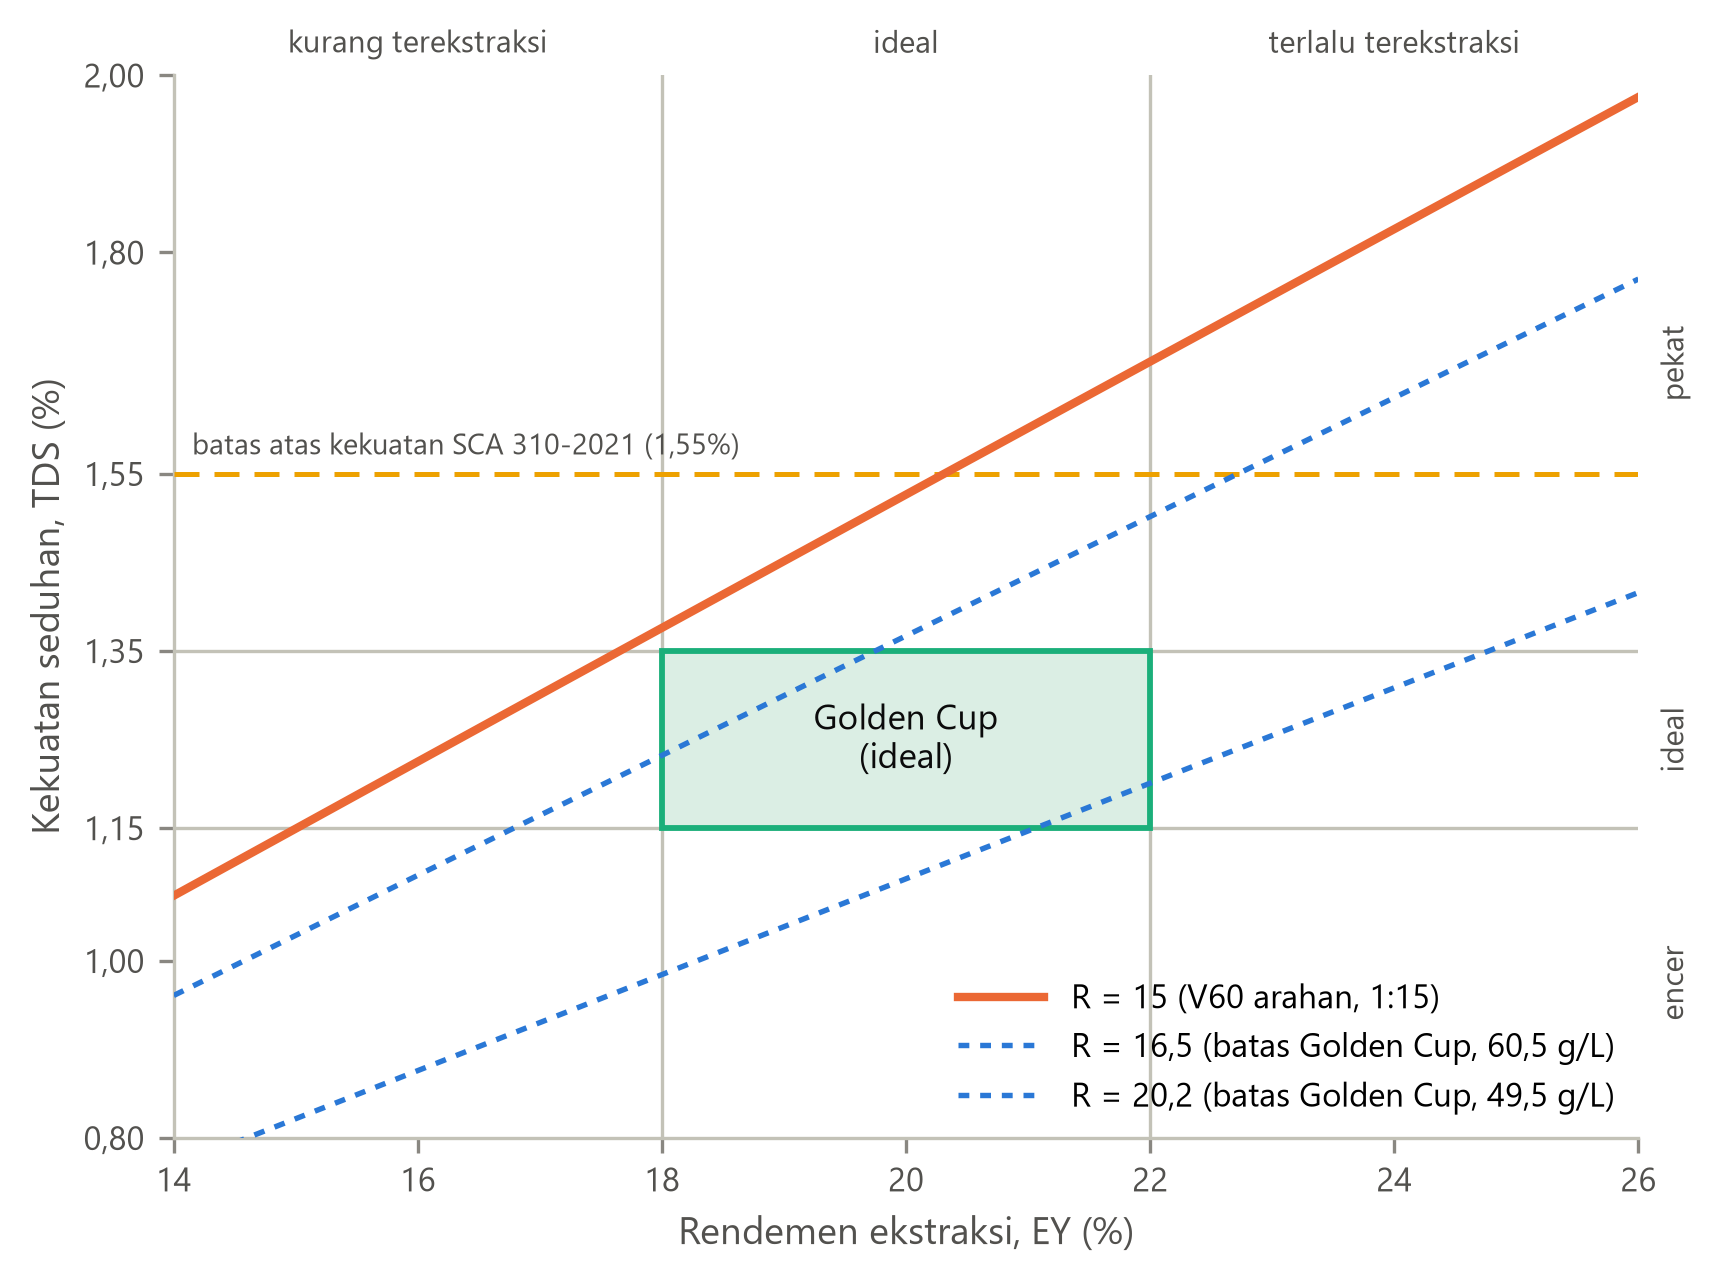
\includegraphics[width=0.78\textwidth]{pic/bagan_kendali_seduh.png}
\caption{Bagan Kendali Seduh dengan Kotak \textit{Golden Cup} dan Garis Rasio Seduh}
\label{fig:bagan-kendali}
\end{figure}

Kotak ideal bukan batas mutlak. Pada kopi tetes dengan sembilan kombinasi TDS dan PE, 21 dari 30 atribut sensori berbeda nyata antarseduhan dan rasa manis berbanding terbalik dengan TDS \citep*{frost2020effects}. Preferensi 118 konsumen kopi hitam tersebar pada rentang kekuatan dan rendemen yang lebar dan membentuk dua segmen yang preferensinya paling dipengaruhi TDS \citep*{cotter2020consumer}, dan rasa asam berkorelasi kuat dengan keasaman tertitrasi yang berkorelasi linier dengan TDS \citep*{batali2021titratable}. Sintesis studi-studi tersebut menghasilkan bagan kendali seduh versi baru, yaitu bagan sensori, bagan konsumen dengan dua klaster preferensi, gabungan keduanya, dan bagan ringkas \citep{guinard2023new}. Suhu air ternyata kurang menentukan: pada kopi tetes dengan target TDS dan PE yang sama pada 87, 90, dan 93~$^\circ$C, suhu seduh tidak berdampak berarti terhadap profil sensori \citep*{batali2020brew}. Karena itu, koreksi seduhan pada sistem pakar Takar diarahkan lebih dahulu ke TDS dan EY melalui rasio, gilingan, dan waktu kontak, dengan suhu air sebagai tuas terakhir.

\subsubsection{Espreso}
\label{subsubsec:espreso}

Espreso dibuat dengan mendorong air panas bertekanan melalui kopi giling halus yang dipadatkan. \citet{cameron2020systematically} menyebutnya sebagai format kopi yang paling rentan terhadap variasi: rendemennya memuncak pada pengaturan gilingan tertentu dan turun pada gilingan yang sangat kasar maupun halus; penurunan pada gilingan halus mereka tafsirkan sebagai petunjuk kuat adanya aliran tidak homogen yang menurunkan reprodusibilitas dan membuang bahan baku. \citet*{schmieder2023influence} mendefinisikan rasio seduh espreso sebagai perbandingan massa kopi giling di dalam \textit{puck} terhadap massa espreso yang terekstraksi ke cangkir:
\begin{equation}
\mathrm{BR} = \frac{m_{\mathrm{kopi}}}{m_{\mathrm{espreso}}},
\label{eq:rasio-espreso}
\end{equation}
dengan $m_{\mathrm{kopi}}$ dosis kopi giling (g) dan $m_{\mathrm{espreso}}$ massa espreso di cangkir (g). Dengan definisi ini, \textit{ristretto} memiliki BR 1/1, espreso BR 1/2, dan \textit{lungo} BR 1/3. Orientasinya berlawanan dengan Persamaan~\eqref{eq:rasio-seduh}, sehingga kedua besaran tidak boleh dicampur; Takar menyimpan kebalikannya, yaitu rasio hasil $1/\mathrm{BR}$ yang bernilai 2 untuk espreso 1:2, sebagai konvensi penulis. Kekuatan espreso 8--12\% disebut tipikal, dan waktu ekstraksinya diatur dengan menghaluskan atau mengasarkan gilingan \citep{moroney2019analysing}. Pengaruh gilingan, laju alir, dan suhu terhadap massa komponen di dalam cangkir tergolong kecil dibandingkan pengaruh perbedaan massa total minuman yang diekstrak \citep*{schmieder2023influence}, dan bagan kendali seduh kinetik untuk espreso juga menunjukkan bahwa rasio seduh lebih berpengaruh terhadap komposisi kopi daripada suhu atau laju alir \citep*{pannusch2024modelbased}. Penulis menyimpulkan bahwa satu \textit{shot} espreso sebaiknya diperlakukan sebagai satuan resep yang tetap, sehingga ukuran minuman diubah dengan menambah atau mempertahankan jumlah \textit{shot} utuh (Subbab~\ref{subsec:penskalaan}). Arahan tidak menetapkan dosis, massa hasil, dan waktu ekstraksi espreso, sehingga nilainya ditetapkan sebagai asumsi pada Bab~\ref{bab:metode}; arahan hanya mengatur urutan tuang, yaitu air panas lebih dahulu pada Long Black agar \textit{crema} bertahan dan sebaliknya pada Americano.

\subsubsection{\texorpdfstring{\textit{Pour Over}}{Pour Over} V60 dan Susu}
\label{subsubsec:v60}

\textit{Pour over} adalah seduhan perkolasi manual: air dituang bertahap di atas kopi giling di dalam corong berkertas saring. Arahan menetapkan resep V60 untuk biji \textit{single origin} Gayo, Toraja, Flores, dan Ethiopia dengan 15~g kopi untuk 225~ml air, gilingan \textit{medium-fine}, dan suhu air 90--92~$^\circ$C, dengan tahapan \textit{blooming} 45~ml air yang didiamkan 30--45~detik untuk melepaskan karbon dioksida, penuangan melingkar hingga 130~ml pada menit ke-1:00, penuangan hingga 225~ml pada menit ke-1:30, dan penetesan yang selesai pada menit ke-2:30 sampai 3:00. Karena target tuangnya kumulatif, seluruh target harus ikut diskalakan ketika dosis berubah. Tabel~\ref{tab:parameter-seduh} membandingkan parameter arahan dengan literatur. Rentang praktik barista dan penyeduh rumahan di Cianjur yang memakai corong V60 menempatkan rasio 1:14--1:16 dengan waktu 2:30--3:00 pada gilingan \textit{medium} dan menyebut \textit{blooming} sekitar 30--45~detik \citep*{bramantoro2025optimization}, walaupun rentang dari sejumlah kecil seduhan itu merupakan bukti praktik, bukan standar. Untuk gilingan \textit{fine-medium}, yang paling dekat dengan gilingan \textit{medium-fine} pada arahan, sumber yang sama mencatat rasio 1:12--1:14, waktu 2--3~menit, dan suhu 86--88~$^\circ$C, sedangkan suhu 90--92~$^\circ$C hanya muncul pada gilingan \textit{medium-coarse}; kombinasi parameter arahan tidak sepadan dengan satu baris praktik tersebut. Gas yang dilepaskan saat \textit{blooming} berkaitan dengan CO\textsubscript{2} yang terbentuk saat sangrai dan dilepaskan lebih mendadak saat penggilingan dan ekstraksi \citep{smrke2017timeresolved}; kaitannya dengan langkah \textit{blooming} adalah inferensi penulis.

\begin{table}[!htb]
\centering
\caption{Parameter Penyajian pada Arahan dan Nilai Acuan dari Literatur}
\label{tab:parameter-seduh}
{\small
\setstretch{1.0}
\begin{tabular}{@{}>{\raggedright\arraybackslash}p{2.5cm}>{\raggedright\arraybackslash}p{3.5cm}>{\raggedright\arraybackslash}p{5.7cm}>{\raggedright\arraybackslash}p{1.3cm}@{}}
\toprule
\textbf{Parameter} & \textbf{Arahan Penelitian} & \textbf{Nilai Acuan} & \textbf{Sumber} \\
\midrule
\multicolumn{4}{@{}l}{\textit{V60 / pour over}} \\
Rasio seduh & 1:15 (15~g : 225~ml) & 55~g/l $\pm$ 10\%, setara 1:16,5--1:20,2\textsuperscript{a} & (1) \\
Suhu air & 90--92~$^\circ$C & 93,0 $\pm$ 3~$^\circ$C (air, SCAA); 90--96~$^\circ$C (campuran kopi dan air, SCA 310-2021) & (1), (2) \\
\textit{Blooming} & 45~ml, 30--45~detik & 30--45~detik & (3) \\
Waktu seduh & Selesai 2:30--3:00 & 2:30--3:00 (gilingan \textit{medium})\textsuperscript{b} & (3) \\
TDS; EY & Tidak ditetapkan & 1,15--1,35\% atau 1,15--1,55\%; 18--22\% & (1), (2) \\
\addlinespace
\multicolumn{4}{@{}l}{\textit{Espreso}} \\
Rasio seduh & Tidak ditetapkan & BR 1/2 (\textit{ristretto} 1/1, \textit{lungo} 1/3) & (4) \\
TDS; EY & Tidak ditetapkan & 8--12\% (tipikal); 18--22\% & (5) \\
\addlinespace
\multicolumn{4}{@{}l}{\textit{Susu}} \\
Suhu \textit{steaming} & 60--65~$^\circ$C & Optimum busa 50--60~$^\circ$C; nutrisi tidak terpengaruh pada 60--65~$^\circ$C & (6), (7) \\
Busa & Latte sekitar 1~cm; cappuccino 1,5--2~cm & Susu pasteurisasi membentuk busa lebih stabil daripada UHT & (6), (7) \\
\bottomrule
\end{tabular}}

\vspace{3pt}
{\footnotesize\raggedright Sumber: (1) \citet*{scaa2015golden}; (2) \citet*{sca2022home}; (3) \citet*{bramantoro2025optimization}; (4) \citet*{schmieder2023influence}; (5) \citet{moroney2019analysing}; (6) \citet{klimanova2022effect}; (7) \citet{santini2023effects}. \textsuperscript{a}\,Dihitung penulis dengan anggapan 1~ml air bermassa 1~g. \textsuperscript{b}\,Untuk gilingan \textit{fine-medium}, sumber (3) mencatat 1:12--1:14, 2--3~menit, dan 86--88~$^\circ$C; suhu 90--92~$^\circ$C hanya muncul pada gilingan \textit{medium-coarse}.\par}
\end{table}

Menurut arahan, Caffè Latte memakai susu segar yang di-\textit{steam} hingga 60--65~$^\circ$C sampai bertekstur lembut dengan \textit{microfoam} sekitar 1~cm, sedangkan Cappuccino memakai busa yang lebih tebal, sekitar 1,5--2~cm, di cangkir 150--180~ml. Busa susu dapat dilemahkan oleh lemak, fosfolipid, asam lemak bebas, dan gliserida parsial \citep*{huppertz2010foaming}. Pada \textit{steaming} dengan mesin espreso, busa dari susu utuh pasteurisasi cenderung lebih stabil dan suhu akhir optimumnya 50--60~$^\circ$C \citep{klimanova2022effect}, sedangkan mutu nutrisi susu tampak tidak terpengaruh pada 60--65~$^\circ$C tetapi menurun pada suhu yang lebih tinggi \citep{santini2023effects}. Rentang arahan dengan demikian sedikit melampaui suhu optimum busa, tetapi masih pada rentang yang tidak menurunkan mutu nutrisi, sehingga Takar tetap memakainya sebagai SOP kedai. Susu yang di-\textit{steam} bertambah volumenya karena busa, sehingga kalkulator memerlukan faktor ekspansi susu yang ditetapkan sebagai asumsi. Minuman dingin dan nonkopi menambahkan dua jenis pengetahuan: pengetahuan volume, misalnya Ice Brown Sugar Shaken Espresso yang berisi dua \textit{shot} espreso, 20~ml \textit{brown sugar syrup}, es batu secukupnya, dan susu hingga penuh (\textit{top up}); dan pengetahuan urutan, misalnya matcha pada Iced Matchagato yang dilarutkan lebih dahulu dengan air hangat agar tidak menggumpal dan Signature Pandan Latte yang disusun berlapis dengan espreso di atas. Pengetahuan pertama ditangani kalkulator penskalaan, sedangkan pengetahuan kedua disimpan sebagai langkah SOP.

%-----------------------------------------------------------------------------%
\subsection{Penskalaan Resep dan Faktor Konversi}
\label{subsec:penskalaan}

Penskalaan resep adalah penyesuaian takaran resep standar terhadap jumlah atau ukuran sajian yang berbeda dari resep asal, sedangkan hasil (\textit{yield}) menyatakan jumlah total yang dihasilkan resep. Cara yang paling umum adalah metode faktor konversi \citep*{bccook2015basic}:
\begin{equation}
f = \frac{Y_{\mathrm{butuh}}}{Y_{\mathrm{resep}}}, \qquad Y = n_{\mathrm{porsi}} \times s_{\mathrm{porsi}},
\label{eq:faktor-konversi}
\end{equation}
dengan $f$ faktor konversi, $Y_{\mathrm{butuh}}$ hasil yang dibutuhkan, $Y_{\mathrm{resep}}$ hasil resep asal, $n_{\mathrm{porsi}}$ jumlah porsi, dan $s_{\mathrm{porsi}}$ ukuran porsi. Setiap bahan kemudian dikalikan dengan faktor yang sama \citep*{bccook2015basic}:
\begin{equation}
q_i^{\mathrm{baru}} = f \times q_i^{\mathrm{asal}},
\label{eq:skala-linier}
\end{equation}
dengan $q_i^{\mathrm{asal}}$ dan $q_i^{\mathrm{baru}}$ takaran bahan ke-$i$ sebelum dan sesudah konversi; bentuk simbolik ini dituliskan penulis dari langkah prosedur dan tabel contoh pada sumber. Penelitian ini menyebut kedua persamaan tersebut sebagai penskalaan linier. Pada kalkulator Takar, $f$ adalah perbandingan volume cangkir tujuan terhadap cangkir dasar, atau perbandingan dosis baru terhadap dosis dasar untuk resep berbasis dosis seperti V60, sedangkan jumlah cangkir mengalikan takaran per cangkir.

Penskalaan linier sederhana, tetapi tidak selalu tepat. Sumber yang sama mengingatkan bahwa bumbu harus dinaikkan dengan hati-hati, waktu pengolahan dapat berubah bila peralatannya berbeda, dan penyesuaian halus hanya dapat dipelajari dari pengalaman, sehingga resep hasil konversi perlu diuji; cairan berkadar gula tinggi seperti sirup juga dianjurkan ditakar berdasarkan berat \citep*{bccook2015basic}. Bar kopi memiliki batasan khasnya sendiri, yang dirangkum penulis pada Tabel~\ref{tab:masalah-penskalaan}. Espreso diekstrak per \textit{shot} utuh, dan massa minuman espreso lebih menentukan komposisi di cangkir daripada gilingan, laju alir, dan suhu \citep*{schmieder2023influence}, sehingga faktor 1,25 tidak dapat dijalankan sebagai 1,25 \textit{shot}; pola ukuran menu sebuah jaringan kedai kopi besar juga bertingkat, bukan proporsional (Tabel~\ref{tab:pola-shot} pada Bab~\ref{bab:pendahuluan}). Susu yang diisi hingga penuh harus dikurangi ketika \textit{shot} ditambah agar minuman tidak meluap. Air dan target tuang V60 harus mengikuti dosis agar rasio 1:15 tetap, karena rasio seduh menentukan kekuatan seduhan \citep*{liang2021equilibrium}; dosis 20~g menuntut target tuang 60; 173,3; dan 300~ml. Hasil perkalian seperti 173,33~ml juga tidak dapat ditakar dengan alat di bar, dan pembulatan yang tidak konsisten membuat total beberapa cangkir berbeda dari jumlah takaran per cangkirnya.

\begin{table}[!htb]
\centering
\caption{Masalah Penskalaan Linier pada Resep Minuman Kopi}
\label{tab:masalah-penskalaan}
{\small
\setstretch{1.0}
\begin{tabular}{@{}>{\raggedright\arraybackslash}p{2.3cm}>{\raggedright\arraybackslash}p{3.4cm}>{\raggedright\arraybackslash}p{3.7cm}>{\raggedright\arraybackslash}p{3.6cm}@{}}
\toprule
\textbf{Masalah} & \textbf{Contoh dari Resep Arahan} & \textbf{Akibat Penskalaan Linier} & \textbf{Arah Penanganan} \\
\midrule
Bahan diskret & Caffè Latte: 1 \textit{shot}, cangkir 200--250~ml & Cangkir 200 ke 250~ml memberi $f = 1{,}25$, yaitu 1,25 \textit{shot} & \textit{Shot} dibulatkan ke \textit{shot} utuh atau mengikuti tabel ukuran \\
\addlinespace
Kapasitas cangkir & Ice Brown Sugar Shaken Espresso: susu \textit{top up} & Tambahan \textit{shot} tanpa mengurangi susu membuat minuman meluap & Susu dihitung sebagai sisa volume cangkir \\
\addlinespace
Rasio seduh & V60: 15~g : 225~ml; target tuang 45, 130, 225~ml & Rasio bergeser bila dosis dan air dibulatkan terpisah & Air dan target tuang dihitung dari dosis akhir dikali rasio \\
\addlinespace
Presisi takar & Sirup 20~ml, susu 150~ml & Takaran pecahan; total tidak sama dengan per cangkir dikali jumlah cangkir & Pembulatan ke presisi alat per cangkir, lalu dikalikan jumlah cangkir \\
\addlinespace
Pengubah pesanan & Kemanisan, tambahan \textit{shot}, penggantian susu atau biji & Pengubah ikut dikalikan faktor atau tidak menyesuaikan komponen lain & Pengubah diterapkan pada komponen sasarannya saja \\
\addlinespace
Es pada minuman dingin & Es batu ``secukupnya'' & Es tidak bertakaran dan volumenya tidak diperhitungkan & Massa es dan volumenya ditetapkan sebagai asumsi \\
\bottomrule
\end{tabular}}
\end{table}

Penanganan setiap masalah bergantung pada sifat komponennya: sebagian proporsional terhadap faktor, sebagian tetap, sebagian diskret, sebagian mengikuti rasio terhadap komponen lain, dan sebagian mengisi sisa volume cangkir. Penskalaan yang memperhatikan sifat-sifat ini disebut penskalaan berbasis batasan (\textit{constraint-aware scaling}); aturannya dirumuskan penulis sebagai Algoritma~\ref{alg:penskalaan} pada Bab~\ref{bab:metode}, sedangkan penskalaan linier menjadi pembanding untuk menguji H1. Penelitian lain memakai penskalaan per porsi dengan penggantian bahan \citep*{benita2026web} atau memprediksi kuantitas bahan dari konteks resep dengan model bahasa \citep{choi2023kitchenscale}. Pendekatan berbasis data tidak menjamin batasan eksplisit seperti \textit{shot} utuh, sedangkan aturan deterministik membuat setiap takaran dapat ditelusuri ke aturan pembentuknya dan diuji terhadap batasan praktis.

%-----------------------------------------------------------------------------%
\subsection{Pengendalian Persediaan Bahan Baku}
\label{subsec:persediaan}

Pengendalian persediaan bertujuan menjaga agar bahan baku cukup untuk melayani permintaan tanpa ditimbun berlebihan. Buku ajar \citet*{silver2016inventory} membahasnya mulai dari model peramalan dan kuantitas pesanan hingga barang mudah rusak dan \textit{material requirements planning} (MRP). Pada kedai kopi di Indonesia, pencatatan di atas kertas dilaporkan menimbulkan data yang tidak akurat, pemesanan ulang yang terlambat, serta kehabisan dan kelebihan stok \citep*{taufiq2025implementation}. Takar mencatat persediaan dengan buku besar stok (\textit{stock ledger}), yaitu daftar pergerakan yang hanya dapat ditambah; setiap pergerakan menyimpan bahan, jenis pergerakan, kuantitas bertanda, dan saldo setelah pergerakan, sedangkan \textit{stock opname} dicatat sebagai penyesuaian sebesar selisih hitung fisik dan saldo sistem. Rancangan ini menerapkan gagasan jejak audit yang juga dipakai sistem stok kafe \citet*{abdur2026sistem}.

Dengan BOM resep, setiap produksi yang dicatat diterjemahkan langsung menjadi pemakaian bahan, mengikuti logika MRP yang menerjemahkan jadwal produksi barang jadi menjadi kebutuhan komponennya dan pernah dipakai untuk merencanakan bahan baku menu pasien dari hasil peramalan \citep*{sri2021raw}. Bila $\hat{y}_{m}(h)$ adalah ramalan permintaan menu $m$ pada hari ke-$h$ dan $b_{mj}$ takaran bahan $j$ per porsi menu $m$, kebutuhan bahan $j$ adalah
\begin{equation}
D_j(h) = \sum_{m} \hat{y}_{m}(h)\, b_{mj}.
\label{eq:ledakan-bom}
\end{equation}
Persamaan~\eqref{eq:ledakan-bom} dirumuskan penulis berdasarkan konsep BOM \citep{kamal2021bill} dan MRP \citep*{sri2021raw}; subresep seperti \textit{shot} espreso diuraikan lebih dahulu menjadi bahan dasarnya. Pendekatan ini berbeda dengan \citet*{piewthongngam2026aienabled} yang mengubah ramalan penjualan menjadi kebutuhan bahan melalui rasio pemakaian historis.

Keputusan persediaan klasik menyangkut berapa banyak dan kapan memesan. Pertanyaan pertama berakar pada pertimbangan \citet*{harris1990many} bahwa bunga atas modal yang tertanam dalam persediaan membatasi jumlah maksimum yang menguntungkan untuk dibuat sekaligus, sedangkan biaya persiapan menentukan jumlah minimumnya; pada sebuah kedai kopi di Indonesia, \textit{economic order quantity} (EOQ) bersama \textit{safety stock} dan \textit{reorder point} (ROP) menurunkan frekuensi pemesanan bahan kopi susu dari 162 menjadi 20 kali per tahun \citep*{nurhalizapratiwi2025analisis}. Takar tidak menghitung EOQ, dan kuantitas pesanannya dibulatkan ke ukuran kemasan. Untuk pertanyaan kedua, persediaan memerlukan stok pengaman (\textit{safety stock}) karena permintaan dan waktu tunggu pemasok (\textit{lead time}) tidak pasti; variabilitas permintaan, \textit{lead time} yang panjang, periode risiko, dan tingkat layanan yang tinggi masing-masing memperbesar stok pengaman \citep*{yigit2023novel}. Pada sistem persediaan Kava Coffee Shop, stok pengaman dihitung sebagai \citep*{taufiq2025implementation}
\begin{equation}
\mathrm{SS} = Z \times \sigma_L = Z\,\sigma_d\sqrt{L},
\label{eq:safety-stock}
\end{equation}
dengan $Z$ nilai distribusi normal baku sesuai tingkat layanan (misalnya 1,65 untuk 95\%), $\sigma_d$ simpangan baku permintaan harian, $\sigma_L$ simpangan baku permintaan selama \textit{lead time}, dan $L$ \textit{lead time} dalam hari; faktor $\sqrt{L}$ muncul karena ragam permintaan harian yang saling bebas selama $L$ hari adalah $L\sigma_d^2$. Takar mengganti $\sigma_d$ dengan simpangan baku galat ramalan harian tingkat bahan dari \textit{backtest}, karena bagi sistem berbasis ramalan yang tidak pasti adalah selisih ramalan dan permintaan aktual; \citet*{lauren2026optimizing} juga memasukkan galat ramalan ke perhitungan stok pengaman.

Pada kebijakan peninjauan kontinu, pesanan dilakukan ketika stok turun sampai titik pemesanan ulang (ROP) \citep*{taufiq2025implementation}:
\begin{equation}
\mathrm{ROP} = \mathrm{SS} + L \times \bar{d},
\label{eq:rop}
\end{equation}
dengan $\bar{d}$ rata-rata pemakaian bahan per hari, sehingga $L \times \bar{d}$ adalah permintaan yang diperkirakan selama menunggu pesanan datang. Persamaan~\eqref{eq:rop} dengan rata-rata historis menjadi dasar pembanding ``ROP statis'' pada simulasi \textit{restock} (H4). Pada kebijakan peninjauan periodik $(R, S)$, posisi persediaan diperiksa setiap $R$ hari dan dinaikkan kembali ke tingkat \textit{order-up-to} $S$ \citep*{yigit2023novel}:
\begin{equation}
S = \bar{d}\,(R + L) + \mathrm{SS}, \qquad Q = S - \mathrm{IP},
\label{eq:order-up-to}
\end{equation}
dengan $R + L$ periode risiko, $Q$ kuantitas pesanan, dan IP posisi persediaan, yaitu stok di tangan ditambah pesanan dalam perjalanan; bagian $Q = S - \mathrm{IP}$ dituliskan penulis dari pernyataan sumber bahwa tingkat stok dinaikkan ke tingkat pesanan. Untuk barang mudah rusak yang kebijakan optimalnya sangat rumit, kebijakan \textit{base-stock} sederhana semacam ini terbukti optimal secara asimtotik ketika umur produk, besar populasi permintaan, atau biaya penalti membesar \citep*{bu2023asymptotic}. Stok pengaman kebijakan periodik semestinya dihitung atas periode risiko $R + L$; Takar menyederhanakannya dengan $\sqrt{L}$, dan sensitivitas terhadap $\sqrt{L + R}$ diperiksa pada Bab~\ref{bab:hasil}.

Dalam Takar, rata-rata $\bar{d}$ diganti dengan jumlah ramalan kebutuhan bahan:
\begin{equation}
\mathrm{ROP}_j = \sum_{h=1}^{L} D_j(h) + \mathrm{SS}_j, \qquad S_j = \sum_{h=1}^{L+R} D_j(h) + \mathrm{SS}_j,
\label{eq:restock-ramalan}
\end{equation}
dengan $j$ indeks bahan. Persamaan~\eqref{eq:restock-ramalan} dirumuskan penulis berdasarkan \citet*{taufiq2025implementation} dan \citet*{yigit2023novel} dan kembali ke bentuk sumbernya bila permintaan rata-rata konstan; aplikasi lalu merekomendasikan $\max(0, S_j - \text{stok di tangan})$ yang dibulatkan ke atas ke ukuran kemasan. Integrasi ini menjawab kritik \citet*{goltsos2022inventory} bahwa penelitian peramalan sering mengabaikan cara ramalan diubah menjadi keputusan pengisian ulang, sedangkan teori persediaan sering menganggap permintaan sudah diketahui.

Sebagian bahan kedai kopi, seperti susu segar, mudah rusak, dan teori persediaan barang mudah rusak membahas kebijakan pemesanan untuk barang berumur tetap maupun yang meluruh \citep*{nahmias1982perishable}. Tingkat layanan yang lebih tinggi memperbesar stok pengaman, dan stok pengaman yang besar menaikkan peluang barang rusak \citep*{yigit2023novel}, sehingga kebijakan \textit{restock} dinilai dengan beberapa ukuran. Ukuran layanan utamanya adalah \textit{fill rate}, yaitu persentase permintaan yang dilayani langsung dari stok di tangan \citep*{goltsos2022inventory}:
\begin{equation}
\mathrm{FR} = \frac{\sum_{t} D_t^{\mathrm{terlayani}}}{\sum_{t} D_t} \times 100\%,
\label{eq:fill-rate}
\end{equation}
dengan $D_t$ permintaan pada hari $t$ dan $D_t^{\mathrm{terlayani}}$ bagian yang terpenuhi dari stok, yaitu $\min(D_t, \text{stok tersedia})$ pada simulasi dengan anggapan permintaan yang tidak terlayani hilang (\textit{lost sales}); notasi ini dituliskan penulis dari definisi verbal sumber. Ukuran pendampingnya adalah jumlah hari kehabisan stok, rata-rata stok di tangan sebagai proksi biaya simpan dan risiko rusak, serta jumlah pesanan.

%-----------------------------------------------------------------------------%
\subsection{Aplikasi Web, Basis Data, dan Keamanan}
\label{subsec:sistem-web}

Takar dibangun sebagai aplikasi web dengan arsitektur klien--server: peramban pada tablet atau ponsel di bar menjalankan antarmuka pengguna, sedangkan server menjalankan logika bisnis, basis data, dan modul AI, dan keduanya berkomunikasi melalui \textit{application programming interface} (API) berbasis HTTP yang bertukar data JSON. Pemisahan ini membuat antarmuka dan logika server dapat dikembangkan serta diuji secara terpisah. Subbab ini membahas REST API dan \textit{single-page application}, FastAPI dan ekosistem Python, basis data relasional, serta keamanan aplikasi. Pembahasan ditutup dengan \textit{Progressive Web App} yang diusulkan arahan tetapi tidak diimplementasikan.

\subsubsection{REST API dan \texorpdfstring{\textit{Single-Page Application}}{Single-Page Application}}
\label{subsubsec:rest-spa}

\textit{Representational State Transfer} (REST) diperkenalkan \citet*{fielding2000architectural} sebagai gaya arsitektur untuk memandu perancangan arsitektur Web modern, dengan penekanan pada skalabilitas interaksi antarkomponen, keumuman antarmuka, dan penerapan komponen secara independen. Dalam API bergaya REST, data dimodelkan sebagai sumber daya (\textit{resource}) yang dialamatkan dengan URL, misalnya \texttt{/api/recipes/\{id\}}, dan dimanipulasi dengan metode HTTP seperti GET, POST, PUT atau PATCH, dan DELETE. Kepatuhan pada aturan desain REST memengaruhi kemudahan memahami API: dalam eksperimen dengan 105 peserta, versi yang melanggar aturan menghasilkan pemahaman yang lebih buruk secara signifikan untuk 11 dari 12 aturan yang diuji \citep*{bogner2023restful}. Dalam penelitian ini, \textit{single-page application} (SPA) dipahami sebagai aplikasi web yang memuat satu halaman HTML, lalu memperbarui tampilannya dengan JavaScript tanpa memuat ulang halaman sambil mengambil data dari API. Vue.js adalah kerangka kerja JavaScript untuk membangun antarmuka pengguna dengan model pemrograman deklaratif dan berbasis komponen; fitur intinya adalah \textit{declarative rendering} dan reaktivitas, yaitu pelacakan perubahan status secara otomatis dan pembaruan DOM yang efisien, dan Vue dapat dipakai untuk membangun SPA \citep*{vuejs2026introduction}. Sifat reaktif ini dimanfaatkan kalkulator takaran, yang langsung menghitung ulang takaran setiap kali ukuran, jumlah cangkir, kemanisan, atau tambahan \textit{shot} berubah. Hasil perbandingan kinerja Vue dengan kerangka kerja lain bergantung pada rancangan ujinya \citep*{lipski2021comparative, bogusz2024performance}. Karena dipakai pada layar sentuh dan sering dengan satu tangan, antarmuka di bar memerlukan target sentuh yang cukup besar, misalnya 9,2--9,6~mm untuk penggunaan ibu jari satu tangan \citep*{parhi2006target}; Takar menerapkan tata letak responsif dengan target sentuh minimal 44~piksel CSS.

\subsubsection{FastAPI dan Ekosistem Python}
\label{subsubsec:fastapi}

FastAPI adalah kerangka kerja web modern berkinerja tinggi untuk membangun API dengan Python berdasarkan anotasi tipe (\textit{type hints}) standar; FastAPI dibangun di atas Starlette dan Pydantic, kompatibel dengan OpenAPI dan JSON Schema, dan menghasilkan dokumentasi API interaktif secara otomatis \citep*{ramirez2026fastapi}. Anotasi tipe dipakai sekaligus untuk validasi masukan, sehingga pada Takar permintaan yang tidak valid ditolak dengan kode status 422. Dalam uji beban I/O berkonkurensi tinggi, aplikasi FastAPI berbasis \textit{Asynchronous Server Gateway Interface} (ASGI) tetap andal, sedangkan aplikasi Flask (WSGI) yang identik mengalami kegagalan \citep*{alaanzy2026performance}, dan pada uji tolok ukur lain FastAPI mengungguli Django REST Framework dan Flask pada sebagian besar skenario \citep*{bednarz2025benchmarking}. Beban satu gerai kedai kopi jauh lebih ringan daripada skenario tersebut, sehingga kinerja Takar tetap diukur langsung. Pemilihan Python juga didorong ekosistem datanya, yaitu pandas yang menyediakan struktur data untuk komputasi statistik \citep*{mckinney2010data}, NumPy sebagai fondasi komputasi larik \citep{harris2020array}, scikit-learn untuk pembelajaran mesin \citep{pedregosa2011scikitlearn}, statsmodels untuk analisis statistik \citep*{seabold2010statsmodels}, dan mlxtend untuk penambangan pola sering \citep*{raschka2018mlxtend}, sehingga API dan modul AI dapat ditulis dalam satu bahasa.

\subsubsection{Basis Data Relasional, ERD, dan SQLite}
\label{subsubsec:basis-data}

\citet*{codd1970relational} memperkenalkan model relasional berbasis relasi $n$-ari agar pengguna bank data yang besar terlindung dari cara data diorganisasi secara internal, serta memperkenalkan bentuk normal bagi relasi basis data dan menerapkan operasi relasi pada masalah redundansi dan konsistensi. Perancangan basis data dimulai dari model entitas--relasi (\textit{entity--relationship}, ER) yang memodelkan entitas dunia nyata beserta relasinya dengan teknik diagram sebagai alat perancangan \citep*{chen1976entity}; diagramnya dikenal sebagai ERD. ERD Takar (Gambar~\ref{fig:erd} di Bab~\ref{bab:metode}) memodelkan resep, komponen resep, ukuran sajian, bahan, pergerakan stok, produksi, SOP, pengguna, transaksi \textit{dataset}, dan keluaran model AI. Akses dari program dilakukan melalui \textit{object--relational mapping} (ORM) yang memetakan kelas ke tabel dan objek ke baris; pemakaian ORM dapat menambah biaya kinerja \citep*{bednarz2025benchmarking}. Takar memakai SQLAlchemy, yaitu \textit{toolkit} SQL dan ORM untuk Python \citep*{bayer2026sqlalchemy}, serta SQLite sebagai mesin basis data. SQLite telah menjadi mesin basis data yang paling banyak dipasang, antara lain berkat rancangan \textit{in-process} dan format berkas lintas platform, dan terutama dirancang untuk pemrosesan transaksi daring (OLTP) \citep{gaffney2022sqlite}, sehingga memadai untuk penerapan satu gerai pada satu komputer.

\subsubsection{Keamanan: JWT, RBAC, dan Argon2}
\label{subsubsec:keamanan}

Takar memakai JSON Web Token (JWT), yaitu cara ringkas untuk merepresentasikan klaim antara dua pihak yang dapat ditandatangani secara digital atau dilindungi dengan \textit{message authentication code}; klaim \texttt{sub} menyatakan subjek token dan \texttt{exp} waktu ketika token tidak boleh lagi diterima \citep*{jones2015json}. Takar menandatangani token dengan HS256, mengunci algoritma yang diterima saat verifikasi, dan mewajibkan kedua klaim tersebut; kehati-hatian ini perlu karena analisis statis atas 358 aplikasi JWT sumber terbuka menemukan 65,92\% di antaranya memiliki sedikitnya satu kerentanan kriptografi \citep{xu2024jwtkey}. Token diperoleh melalui \textit{resource owner password credentials grant} OAuth~2.0 yang hanya layak bila klien dipercaya pemilik sumber daya \citep*{hardt2012oauth}; pola ini dicontohkan tutorial resmi FastAPI \citep*{ramirez2026fastapi}, tetapi praktik keamanan terkini menyatakan bahwa \textit{grant} tersebut tidak boleh dipakai dan menganjurkan \textit{authorization code grant} dengan PKCE \citep*{lodderstedt2025best}. Takar memakainya karena SPA-nya merupakan klien pihak pertama pada prototipe satu gerai, dan keterbatasan ini dicatat sebagai saran (Subbab~\ref{sec:saran}).

Otorisasi memakai kontrol akses berbasis peran (\textit{role-based access control}, RBAC) yang menyederhanakan administrasi keamanan dengan melekatkan izin pada peran \citep*{sandhu1996rolebased}; Takar memiliki peran manajer, \textit{head barista}, dan barista. OWASP Top 10:2025 menempatkan \textit{broken access control} di peringkat pertama risiko aplikasi web dan menganjurkan kontrol akses yang ditegakkan di sisi server, menolak secara bawaan, dan diuji dalam uji unit dan integrasi \citep*{owasp2025owasp}. Karena itu, Takar memeriksa token di sisi server pada setiap \textit{endpoint} API kecuali login dan pemeriksaan status server, memeriksa peran pada \textit{endpoint} yang dibatasi, serta mengembalikan kode 401 untuk token yang tidak ada atau tidak valid dan 403 untuk peran yang tidak berwenang. OWASP juga menganjurkan penyimpanan kata sandi dengan fungsi \textit{hash} adaptif bergaram seperti Argon2 \citep*{owasp2025owasp}. Argon2 membutuhkan memori yang dapat diatur sehingga penyerang yang menghemat memori menghadapi pertukaran waktu--memori yang sangat mahal, dan tahan terhadap serangan dengan ASIC maupun \textit{botnet} \citep*{biryukov2016argon2}; RFC~9106 menganjurkan varian Argon2id bila serangan kanal samping mungkin terjadi \citep*{biryukov2021argon2}, dan varian inilah yang dipakai Takar.

\subsubsection{\texorpdfstring{\textit{Progressive Web App}}{Progressive Web App} dan Mode Luring}
\label{subsubsec:pwa}

Arahan penelitian mengusulkan \textit{Progressive Web App} (PWA) agar aplikasi dapat dipakai secara luring. PWA dipandang sebagai kemungkinan langkah menuju pengembangan lintas platform dari satu basis kode \citep*{majchrzak2018progressive}, dengan kemampuan luring yang bertumpu pada \textit{service worker} yang dapat mencegat permintaan dan menyimpan pasangan permintaan--respons \citep*{chintala2026service} serta pada basis data sisi klien IndexedDB \citep*{becker2025indexed}. Penelitian ini tidak mengimplementasikan PWA karena perubahan teknologi yang dijelaskan pada Subbab~\ref{sec:latar-belakang}, sehingga Takar memerlukan koneksi ke server lokal selama dipakai di bar. Sinkronisasi data luring, misalnya dengan antrean IndexedDB dan \textit{background sync} \citep*{nugraha2026implementation} atau prinsip perangkat lunak \textit{local-first} \citep*{kleppmann2019localfirst}, menjadi saran pengembangan.

%-----------------------------------------------------------------------------%
\subsection{Kecerdasan Buatan dan Sistem Rekomendasi}
\label{subsec:kecerdasan-buatan}

Istilah kecerdasan buatan (\textit{artificial intelligence}, AI) dipakai dalam penelitian ini secara operasional untuk teknik komputasi yang menghasilkan saran keputusan dari data atau dari pengetahuan pakar yang dikodekan. Definisi kerja ini mencakup dua tradisi. Tradisi pertama adalah sistem berbasis pengetahuan: buku ajar \citet*{russell2021artificial} membahas agen berbasis pengetahuan beserta penalaran \textit{forward chaining} dan \textit{backward chaining}, dan mencatat sistem pakar sebagai salah satu tahap sejarah AI. Tradisi kedua adalah pembelajaran mesin (\textit{machine learning}) yang membangun model dari data untuk masalah terawasi dan tak terawasi \citep{pedregosa2011scikitlearn}; penambangan aturan dari transaksi dan peramalan deret waktu digolongkan penulis ke dalam tradisi ini.

Sistem rekomendasi adalah perangkat lunak dan teknik yang memberi saran tentang \textit{item} yang paling mungkin menarik bagi pengguna tertentu \citep*{ricci2021recommender}. Selain \textit{collaborative filtering} dan \textit{content-based filtering}, terdapat sistem rekomendasi berbasis pengetahuan yang memanfaatkan pengetahuan tentang preferensi pengguna, \textit{item}, dan rekomendasi, dengan rekomendasi yang ditentukan melalui batasan atau kemiripan atribut \citep{uta2024knowledgebased}. Pada rekomendasi berbasis \textit{item}, kemiripan antar-\textit{item} digabungkan untuk menilai kecocokan antara sekumpulan \textit{item} (keranjang) dan setiap kandidat \textit{item} \citep*{deshpande2004itembased}. Dalam kerangka ini, pasangan menu Takar adalah rekomendasi berbasis keranjang dengan aturan asosiasi (Subbab~\ref{subsec:aturan-asosiasi}), rekomendasi \textit{restock} memadukan peramalan permintaan (Subbab~\ref{subsec:peramalan}) dengan kebijakan persediaan, dan koreksi parameter seduh adalah rekomendasi berbasis pengetahuan berupa sistem pakar (Subbab~\ref{subsec:sistem-pakar}), karena pengetahuannya tersedia dalam literatur penyeduhan sedangkan data interaksi yang memadai tidak tersedia. Rekomendasi makanan sendiri merupakan domain yang memerlukan konteks dan pengetahuan domain \citep*{min2020food}; keputusan makan bersifat kompleks dan bergantung pada konteks, sedangkan algoritma rekomendasi standar cenderung memperkuat kebiasaan yang sudah ada \citep*{elsweiler2022food}. Tinjauan sistematis atas 67 studi mengkaji metode, data, dan cara evaluasi sistem rekomendasi makanan \citep*{bondevik2024systematic}, dan pada data kopi, AI telah dipakai untuk memprediksi kesukaan konsumen dari data sensori \citep*{gunning2026aidriven}.

%-----------------------------------------------------------------------------%
\subsection{Aturan Asosiasi}
\label{subsec:aturan-asosiasi}

Penambangan aturan asosiasi diperkenalkan \citet*{agrawal1993mining} untuk basis data transaksi pelanggan yang setiap transaksinya berisi \textit{item} yang dibeli dalam satu kunjungan. Misalkan $I$ adalah himpunan semua \textit{item} (menu) dan $D$ basis data transaksi, dengan setiap transaksi $T \in D$ berupa himpunan $T \subseteq I$. Himpunan $X \subseteq I$ disebut \textit{itemset}, dan aturan asosiasi ditulis $X \rightarrow Y$ dengan $X$ (\textit{antecedent}) dan $Y$ (\textit{consequent}) dua \textit{itemset} yang saling lepas; pada kedai kopi, satu transaksi adalah satu struk, dan aturan $\{\text{latte}\} \rightarrow \{\text{croissant}\}$ menyatakan bahwa pembeli latte cenderung juga membeli croissant. \textit{Support} adalah proporsi transaksi yang memuat seluruh \textit{item} suatu \textit{itemset}, dan \textit{confidence} adalah peluang bersyarat bahwa transaksi yang memuat $X$ juga memuat $Y$ \citep*{agrawal1993mining, brin1997dynamic, sihombing2026analisis}:
\begin{equation}
\mathrm{support}(X) = \frac{\left|\{\, T \in D : X \subseteq T \,\}\right|}{|D|},
\label{eq:support}
\end{equation}
\begin{equation}
\mathrm{confidence}(X \rightarrow Y) = \frac{\mathrm{support}(X \cup Y)}{\mathrm{support}(X)},
\label{eq:confidence}
\end{equation}
dengan $|D|$ jumlah transaksi; \textit{support} aturan $X \rightarrow Y$ adalah $\mathrm{support}(X \cup Y)$, dan notasi himpunan pada Persamaan~\eqref{eq:support} dituliskan penulis dari definisi sumber. \textit{Itemset} dengan \textit{support} tidak kurang dari ambang minimum disebut \textit{itemset} sering (\textit{frequent itemset}). Karena setiap transaksi yang memuat $X \cup \{i\}$ juga memuat $X$, menambah \textit{item} tidak dapat menaikkan \textit{support}, sehingga setiap himpunan bagian dari \textit{itemset} sering juga sering.

\textit{Confidence} mengabaikan seberapa sering $Y$ muncul secara umum \citep*{brin1997dynamic}, sehingga menu yang sangat populer dapat menghasilkan \textit{confidence} tinggi dengan hampir semua \textit{antecedent}. \textit{Lift}, yang oleh \citet*{brin1997dynamic} disebut \textit{interest}, memperbaiki kelemahan ini \citep*{brin1997dynamic, sihombing2026analisis}:
\begin{equation}
\mathrm{lift}(X \rightarrow Y) = \frac{\mathrm{confidence}(X \rightarrow Y)}{\mathrm{support}(Y)} = \frac{\mathrm{support}(X \cup Y)}{\mathrm{support}(X)\,\mathrm{support}(Y)}.
\label{eq:lift}
\end{equation}
Nilai \textit{lift} 1 berarti saling bebas, lebih dari 1 berarti asosiasi positif, dan kurang dari 1 berarti asosiasi negatif; \textit{lift} bersifat simetris sehingga mengukur kemunculan bersama, bukan implikasi \citep*{brin1997dynamic}. Pada \textit{dataset} Bread Basket, misalnya, Bread $\rightarrow$ Coffee memiliki \textit{support} lebih tinggi daripada Cake $\rightarrow$ Coffee tetapi \textit{lift}-nya hanya 0,575 \citep*{sihombing2026analisis}.

Ukuran-ukuran tersebut termasuk ukuran kemenarikan (\textit{interestingness measures}) untuk memilih dan memeringkat pola \citep*{geng2006interestingness}. \textit{Leverage}, yang dikenal sebagai ukuran Piatetsky-Shapiro, adalah selisih antara frekuensi kemunculan bersama yang teramati dan frekuensi harapannya bila $X$ dan $Y$ saling bebas \citep*{geng2006interestingness}, sedangkan \textit{conviction} dirancang \citet*{brin1997dynamic} untuk mengukur implikasi dengan memperhatikan \textit{antecedent} dan \textit{consequent} sekaligus:
\begin{equation}
\mathrm{leverage}(X \rightarrow Y) = \mathrm{support}(X \cup Y) - \mathrm{support}(X)\,\mathrm{support}(Y),
\label{eq:leverage}
\end{equation}
\begin{equation}
\mathrm{conviction}(X \rightarrow Y) = \frac{P(X)\,P(\neg Y)}{P(X, \neg Y)} = \frac{1 - \mathrm{support}(Y)}{1 - \mathrm{confidence}(X \rightarrow Y)},
\label{eq:conviction}
\end{equation}
dengan $P(X) = \mathrm{support}(X)$, $P(\neg Y) = 1 - \mathrm{support}(Y)$, dan $P(X, \neg Y)$ proporsi transaksi yang memuat $X$ tetapi tidak memuat $Y$. \textit{Leverage} bernilai nol untuk \textit{item} yang saling bebas, dan karena sama dengan $\mathrm{support}(X)\,\mathrm{support}(Y)\,(\mathrm{lift} - 1)$, aturan yang jarang terjadi mendapat \textit{leverage} kecil walaupun \textit{lift}-nya besar. \textit{Conviction} bernilai 1 untuk \textit{item} yang tidak berkaitan dan tak hingga untuk aturan yang selalu benar \citep*{brin1997dynamic}; bentuk keduanya setara karena $P(X, \neg Y) = \mathrm{support}(X) - \mathrm{support}(X \cup Y)$, dan bentuk kedua dihitung implementasi Takar.

Penambangan aturan berlangsung dalam dua tahap: menemukan semua \textit{itemset} sering, lalu membentuk aturan dan menyaringnya dengan ambang \textit{confidence} atau ukuran lain. Algoritma bergaya Apriori memakai pendekatan pembangkitan dan pengujian kandidat, yaitu \textit{itemset} kandidat yang lebih panjang dibangkitkan dari \textit{itemset} sering yang lebih pendek, lalu \textit{support}-nya dihitung dengan memindai basis data; pendekatan ini mahal ketika pola sering sangat banyak atau panjang \citep*{han2000mining, han2004mining} dan memerlukan beberapa kali pemindaian data \citep*{brin1997dynamic}. FP-Growth menghindari pembangkitan kandidat: basis data dimampatkan menjadi \textit{frequent-pattern tree} (FP-\textit{tree}), yaitu pohon prefiks yang menyimpan informasi pola sering secara ringkas, lalu pola ditambang melalui pertumbuhan fragmen pola secara \textit{divide and conquer} pada basis data bersyarat. FP-Growth dilaporkan efisien dan skalabel serta sekitar satu orde besaran lebih cepat daripada Apriori \citep*{han2000mining, han2004mining}. Tabel~\ref{tab:apriori-fpgrowth} merangkum perbandingan keduanya.

\begin{table}[!htb]
\centering
\caption{Perbandingan Apriori dan FP-Growth}
\label{tab:apriori-fpgrowth}
{\small
\setstretch{1.0}
\begin{tabular}{@{}>{\raggedright\arraybackslash}p{2.9cm}>{\raggedright\arraybackslash}p{5.1cm}>{\raggedright\arraybackslash}p{5.4cm}@{}}
\toprule
\textbf{Aspek} & \textbf{Apriori} & \textbf{FP-Growth} \\
\midrule
Strategi & Pembangkitan dan pengujian kandidat & Pertumbuhan fragmen pola tanpa kandidat \\
Struktur data & Himpunan \textit{itemset} kandidat & FP-\textit{tree} dan basis data bersyarat \\
Biaya utama & Banyak kandidat dan pemindaian data berulang & Pembentukan dan penambangan FP-\textit{tree} \\
Keluaran & Seluruh \textit{itemset} sering pada ambang yang sama & Seluruh \textit{itemset} sering pada ambang yang sama \\
Kinerja & Acuan pembanding & Sekitar satu orde besaran lebih cepat \\
Contoh pada F\&B & \citet*{nasution2025application}; \citet*{pratama2026automatic} & \citet*{fadillah2021data}; \citet*{pratama2025food}; \citet*{sihombing2026analisis} \\
\bottomrule
\end{tabular}}
\end{table}

Karena kedua algoritma menghasilkan \textit{itemset} sering yang sama pada ambang yang sama, pilihan di antara keduanya adalah soal efisiensi, bukan mutu aturan. Takar memakai FP-Growth dari pustaka mlxtend \citep*{raschka2018mlxtend} pada keranjang menu berbentuk matriks biner (\textit{one-hot}) dan menghitung kelima ukuran pada Persamaan~\eqref{eq:support}--\eqref{eq:conviction}. Rekomendasi untuk suatu pesanan diambil dari aturan yang seluruh \textit{antecedent}-nya ada di pesanan dan \textit{consequent}-nya belum ada, diurutkan menurut \textit{confidence} lalu \textit{lift}, dan slot tersisa diisi menu terpopuler yang ditandai sebagai cadangan. Ambang \textit{support} dan \textit{confidence} dipilih pada potongan validasi dari periode latih saja agar tidak terjadi kebocoran data (Subbab~\ref{subsec:evaluasi-rekomendasi}).

%-----------------------------------------------------------------------------%
\subsection{Peramalan Permintaan}
\label{subsec:peramalan}

Peramalan permintaan memperkirakan nilai deret waktu pada masa depan dari nilai masa lalunya. Misalkan $y_1, \dots, y_T$ adalah penjualan harian suatu menu hingga titik asal ramalan (\textit{forecast origin}) $T$; ramalan untuk $h$ hari ke depan (horizon $h$) ditulis $\hat{y}_{T+h\mid T}$ \citep*{hyndman2021forecasting}. Penjualan harian dapat berpola mingguan; pada sebuah restoran, hari dalam minggu, musim perayaan, dan hari libur tampak memengaruhi penjualan \citep*{pazhamannil2025optimization}. Metode paling sederhana adalah metode naif dan naif musiman (\textit{seasonal naive}) \citep*{hyndman2021forecasting}:
\begin{equation}
\hat{y}_{T+h\mid T} = y_T, \qquad \hat{y}_{T+h\mid T} = y_{T+h-m(k+1)}, \quad k = \left\lfloor \frac{h-1}{m} \right\rfloor,
\label{eq:naive}
\end{equation}
dengan $y_T$ observasi terakhir, $m$ periode musiman ($m = 7$ untuk data harian berpola mingguan), dan $k$ bagian bulat dari $(h-1)/m$. Naif musiman memakai nilai pada hari yang sama di minggu terakhir dan menjadi pembanding H3 serta penskala MASE.

Rata-rata bergerak sederhana (\textit{simple moving average}, SMA) dengan jendela $w$ dipakai sebagai ramalan datar; bentuknya dirumuskan penulis berdasarkan \citet*{lauren2026optimizing}:
\begin{equation}
\hat{y}_{T+h\mid T} = \frac{1}{w}\sum_{j=0}^{w-1} y_{T-j}, \qquad h = 1, 2, \dots,
\label{eq:ma}
\end{equation}
dengan $w$ panjang jendela ($w = 7$ hari pada Takar) dan $y_{T-j}$ observasi $j$ hari sebelum titik asal. \citet*{lauren2026optimizing} menuliskan rata-rata bergerak ke belakang ini sebagai indikator tren dan memakai SMA sebagai pembanding, tetapi tidak menuliskan pemakaiannya sebagai ramalan datar dalam persamaan tersendiri. Rata-rata bergerak terpusat untuk dekomposisi deret waktu \citep*{hyndman2021forecasting} tidak dapat dipakai sebagai ramalan karena memerlukan observasi masa depan.

Pemulusan eksponensial sederhana (\textit{simple exponential smoothing}, SES) memberi bobot yang menurun secara eksponensial pada observasi yang makin lama \citep*{hyndman2021forecasting}:
\begin{equation}
\begin{aligned}
\hat{y}_{T+1\mid T} &= \alpha y_T + \alpha(1-\alpha) y_{T-1} + \alpha(1-\alpha)^2 y_{T-2} + \cdots \\
\hat{y}_{t+h\mid t} &= \ell_t, \qquad \ell_t = \alpha y_t + (1-\alpha)\,\ell_{t-1},
\end{aligned}
\label{eq:ses}
\end{equation}
dengan $\alpha \in [0, 1]$ parameter pemulusan dan $\ell_t$ level pada waktu $t$; baris pertama adalah bentuk rata-rata berbobot dan baris kedua bentuk komponen. Metode Holt mengembangkan pemulusan eksponensial untuk tren dan data musiman \citep*{holt2004forecasting}, dan \citet*{winters1960forecasting} merancang peramalan penjualan per produk yang cepat, murah, dan responsif untuk pengendalian persediaan sambil menguji metode Holt dengan data empiris; gabungannya dikenal sebagai metode Holt-Winters. Tinjauan \citet*{gardner2006exponential} menyimpulkan bahwa tren teredam (\textit{damped trend}) yang diterapkan pada setiap deret masih sulit dikalahkan. Versi aditif dengan tren teredam dan musim aditif yang dipakai penelitian ini adalah \citep*{hyndman2021forecasting}
\begin{equation}
\begin{aligned}
\hat{y}_{t+h\mid t} &= \ell_t + \phi_h b_t + s_{t+h-m(k+1)} \\
\ell_t &= \alpha\,(y_t - s_{t-m}) + (1-\alpha)(\ell_{t-1} + \phi b_{t-1}) \\
b_t &= \beta^{*}(\ell_t - \ell_{t-1}) + (1-\beta^{*})\,\phi b_{t-1} \\
s_t &= \gamma\,(y_t - \ell_{t-1} - \phi b_{t-1}) + (1-\gamma)\,s_{t-m},
\end{aligned}
\label{eq:holt-winters}
\end{equation}
dengan $b_t$ tren, $s_t$ komponen musiman, $\beta^{*}$ dan $\gamma$ parameter pemulusan tren dan musim, $\phi \in (0, 1)$ parameter peredam, $\phi_h = \phi + \phi^2 + \dots + \phi^h$, serta $m$ dan $k$ seperti pada Persamaan~\eqref{eq:naive}. Peredam membuat tren ramalan melandai sehingga ramalan horizon panjang tidak tumbuh tanpa batas. Implementasi statsmodels \citep*{seabold2010statsmodels} yang dipakai Takar menjalankan persamaan pembaruan yang sama.

Model pembelajaran mesin yang dipakai adalah \textit{gradient boosting}. \citet*{friedman2001greedy} memandang estimasi fungsi sebagai optimasi numerik dalam ruang fungsi; pada setiap iterasi, pohon regresi dicocokkan ke gradien negatif fungsi kerugian (residu semu), lalu ditambahkan ke model dengan laju belajar:
\begin{equation}
F_m(\mathbf{x}) = F_{m-1}(\mathbf{x}) + \nu \cdot \rho_m\, h(\mathbf{x}; \mathbf{a}_m), \qquad 0 < \nu \le 1,
\label{eq:gradient-boosting}
\end{equation}
dengan $F_m$ model setelah iterasi ke-$m$, $h(\mathbf{x}; \mathbf{a}_m)$ pohon regresi berparameter $\mathbf{a}_m$ (bukan horizon $h$), $\rho_m$ besar langkah hasil pencarian garis, dan $\nu$ laju belajar (\textit{shrinkage}). Pada pohon regresi, nilai daun sudah memuat langkah optimal sehingga pembaruannya sering ditulis $\hat{f}(\mathbf{x}) \leftarrow \hat{f}(\mathbf{x}) + \lambda \hat{f}^{b}(\mathbf{x})$ dengan $\lambda$ sebagai laju belajar \citep*{james2021introduction}. Friedman melaporkan bahwa \textit{boosting} pohon regresi kompetitif, sangat tangguh, dan cocok untuk data yang tidak bersih, dan LightGBM mempercepat pelatihannya hingga lebih dari 20 kali dengan akurasi hampir sama \citep{ke2017lightgbm}. Takar memakai HistGradientBoostingRegressor dari scikit-learn \citep{pedregosa2011scikitlearn} sebagai model global, yaitu satu model untuk semua deret menu dan gerai dengan fitur yang tersedia pada titik asal, seperti nilai penjualan beberapa minggu sebelumnya, rata-rata bergerak, hari dalam minggu, dan horizon, sehingga setiap horizon diramalkan langsung (\textit{direct}) dari informasi di titik asal. Pada kompetisi M5 yang meminta ramalan 42.840 deret penjualan unit Walmart \citep*{makridakis2022m5}, pemenangnya merata-ratakan model langsung dan rekursif berbasis LightGBM yang dilatih pada data gabungan \citep*{in2022simple}, dan pendekatan pohon \textit{gradient boosting} mendominasi peringkat atas \citep{januschowski2022forecasting}. Keunggulan itu tidak berlaku umum: pada sebuah restoran di Bangladesh, SES dan metode Croston mengungguli XGBoost \citep*{hossain2025comparative}, sehingga model global selalu dibandingkan dengan metode sederhana.

Akurasi ramalan diukur dari galat ramalan \citep*{hyndman2021forecasting}:
\begin{equation}
e_{T+h} = y_{T+h} - \hat{y}_{T+h\mid T}, \qquad \mathrm{MAE} = \frac{1}{n}\sum_{t=1}^{n} |e_t|, \qquad \mathrm{RMSE} = \sqrt{\frac{1}{n}\sum_{t=1}^{n} e_t^2},
\label{eq:mae-rmse}
\end{equation}
dengan $n$ jumlah galat yang dievaluasi. \textit{Mean absolute error} (MAE) dan \textit{root mean squared error} (RMSE) bergantung pada skala data, dan RMSE memberi bobot lebih besar pada galat besar. Karena menu dan bahan memiliki satuan berbeda, dipakai pula \textit{weighted absolute percentage error} (WAPE) yang membagi jumlah galat mutlak dengan jumlah nilai aktual mutlak \citep*{hewamalage2022forecast}:
\begin{equation}
\mathrm{WAPE} = \frac{\sum_{t} |e_t|}{\sum_{t} |y_t|}.
\label{eq:wape}
\end{equation}
Sumber mendefinisikan WAPE per deret atas horizon, sedangkan penelitian ini melaporkan WAPE keseluruhan atas semua deret, titik asal, dan horizon, sehingga menu yang terjual banyak berbobot lebih besar. WAPE tetap terdefinisi pada deret yang memuat hari tanpa penjualan, berbeda dengan \textit{mean absolute percentage error} (MAPE) yang tak hingga atau tidak terdefinisi ketika nilai aktualnya nol \citep*{hyndman2006another, hewamalage2022forecast}.

\textit{Mean absolute scaled error} (MASE) diusulkan \citet*{hyndman2006another} sebagai ukuran baku untuk membandingkan akurasi di banyak deret; versi musimannya membagi galat dengan MAE ramalan naif musiman pada data latih \citep*{hyndman2021forecasting}:
\begin{equation}
q_j = \frac{e_j}{\dfrac{1}{T-m}\displaystyle\sum_{t=m+1}^{T} |y_t - y_{t-m}|}, \qquad \mathrm{MASE} = \mathrm{mean}(|q_j|),
\label{eq:mase}
\end{equation}
dengan $q_j$ galat terskala dan $T$ panjang data latih. MASE di bawah satu berarti ramalan lebih akurat daripada naif musiman satu langkah pada data latih. Penyebutnya bernilai nol bila deret latih tidak berubah dalam pola musimannya, misalnya menu yang tidak pernah terjual, sehingga ukuran berbasis penskala pembanding gagal pada kasus tersebut \citep*{hewamalage2022forecast}. Bias menunjukkan kecenderungan ramalan terlalu tinggi atau terlalu rendah, dan sumber mendefinisikannya sebagai galat rata-rata (\textit{mean error}, ME) \citep*{hewamalage2022forecast}:
\begin{equation}
\mathrm{ME} = \frac{1}{n}\sum_{t=1}^{n} \left(y_t - \hat{y}_t\right), \qquad \mathrm{bias} = \frac{1}{n}\sum_{t=1}^{n} \left(\hat{y}_t - y_t\right) = -\mathrm{ME}.
\label{eq:bias}
\end{equation}
Menurut konvensi sumber, ME positif berarti ramalan rata-rata terlalu rendah. Skrip evaluasi penelitian ini menghitung bias dengan tanda sebaliknya (bentuk kedua), sehingga bias positif pada Bab~\ref{bab:hasil} berarti ramalan rata-rata terlalu tinggi (\textit{over-forecast}).

Cara membagi data sama pentingnya dengan ukuran galat. Pada evaluasi \textit{rolling origin}, horizon tetap sedangkan titik asal digeser sehingga terbentuk beberapa periode uji, dan model dapat dilatih ulang dengan data baru pada setiap titik asal; skema ini juga disebut validasi silang deret waktu dan dianjurkan bila data cukup tersedia \citep*{hewamalage2022forecast}. Gambar~\ref{fig:rolling-origin} mengilustrasikan skema tersebut. Karena setiap model hanya melihat data hingga titik asalnya, evaluasi ini meniru pemakaian nyata dan mencegah kebocoran informasi dari masa depan. Takar memakai delapan titik asal mingguan dengan horizon tujuh hari (Subbab~\ref{sec:rancangan-eksperimen}).

\begin{figure}[htbp]
\centering
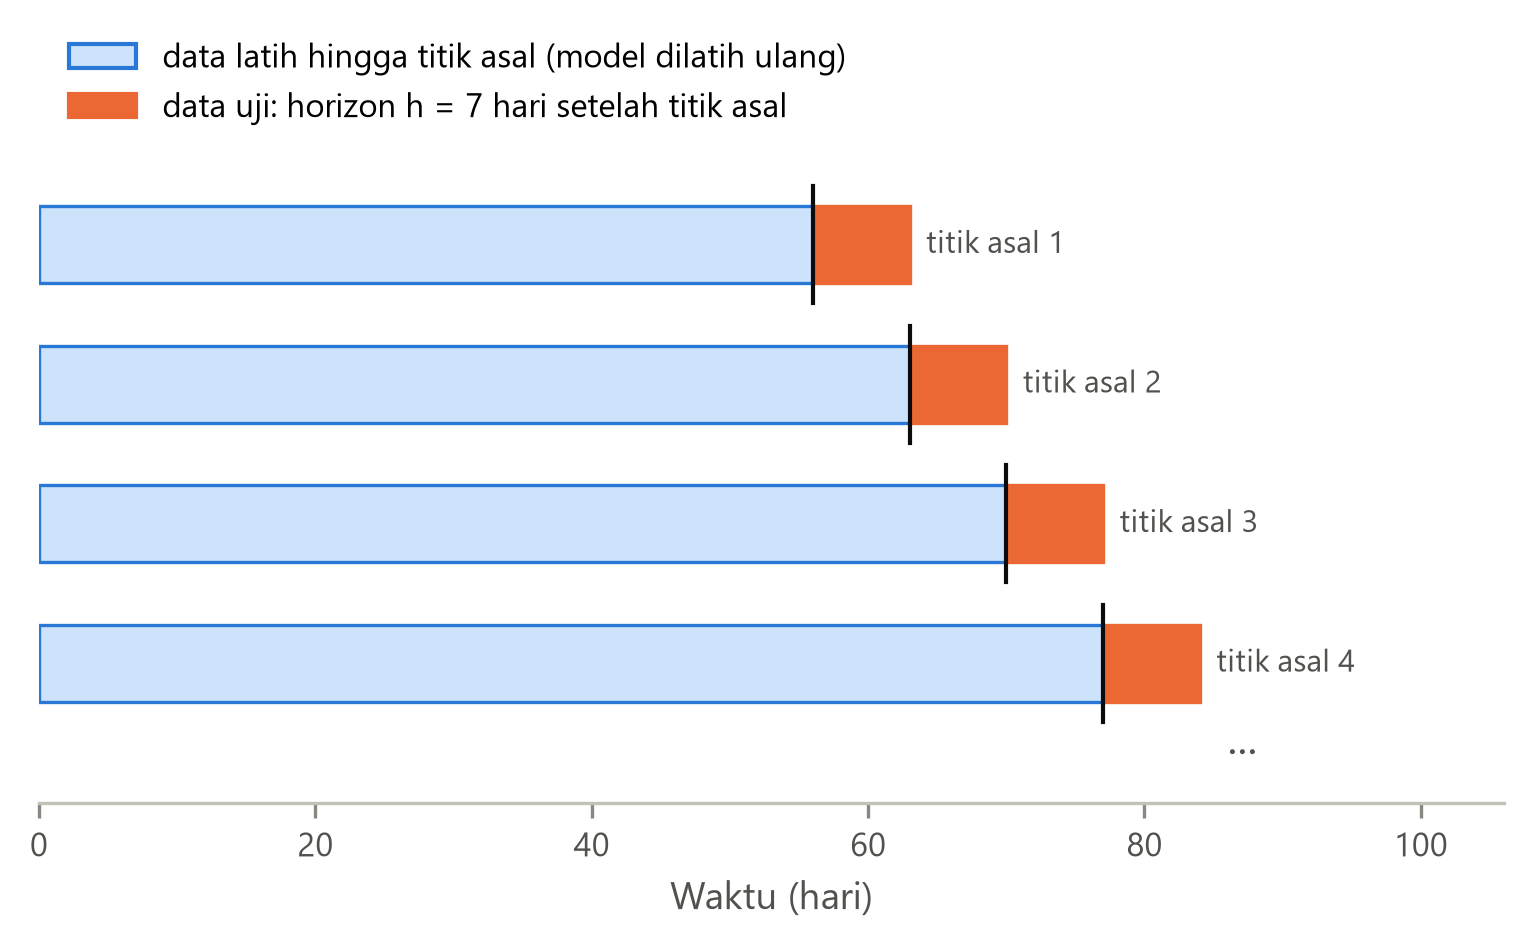
\includegraphics[width=0.78\textwidth]{pic/rolling_origin.png}
\caption{Skema Evaluasi \textit{Rolling Origin}}
\label{fig:rolling-origin}
\end{figure}

%-----------------------------------------------------------------------------%
\subsection{Sistem Pakar dan \texorpdfstring{\textit{Forward Chaining}}{Forward Chaining}}
\label{subsec:sistem-pakar}

Sistem pakar adalah sistem berbasis pengetahuan yang dapat mendukung, dan kadang menggantikan, pakar dalam mengambil keputusan. Komponen penyusunnya adalah basis pengetahuan, mesin inferensi, dan antarmuka pengguna, dan validasinya penting karena banyak sistem pakar dalam literatur tidak divalidasi \citep*{saibene2021expert}. Basis pengetahuan menyimpan pengetahuan domain sebagai aturan produksi JIKA--MAKA (\textit{IF--THEN}), mesin inferensi menerapkan aturan pada fakta untuk menarik kesimpulan, dan antarmuka menerima masukan serta menampilkan kesimpulan. \textit{Backward chaining} menalar dari tujuan menuju fakta pendukungnya, sedangkan \textit{forward chaining} menalar dari fakta yang diketahui: setiap aturan yang seluruh premisnya terpenuhi dijalankan (\textit{fired}), konklusinya ditambahkan ke memori kerja sebagai fakta baru, dan proses diulang hingga tidak ada fakta baru; kedua metode dibahas dalam buku ajar \citet*{russell2021artificial}. Algoritma~\ref{alg:forward-chaining}, yang disusun penulis, menuliskan \textit{forward chaining} dengan jejak aturan sebagaimana dipakai pada penelitian ini. Metode ini cocok untuk diagnosis seduhan karena masukannya berupa data yang dikumpulkan lebih dahulu, yaitu hasil pengukuran dan keluhan rasa, dan sistem perlu menurunkan semua kesimpulan yang relevan dari data itu.

\begin{algorithm}[htbp]
\caption{\textit{Forward Chaining} dengan Jejak Aturan}
\label{alg:forward-chaining}
\begin{algorithmic}[1]
\Require himpunan fakta awal $F$; himpunan aturan $\mathcal{R}$, setiap aturan $r$ memiliki premis $P_r$, konklusi $C_r$, dan prioritas
\Ensure himpunan fakta akhir $F$ dan jejak aturan terpicu $J$
\State $J \gets$ daftar kosong
\Repeat
  \State $\mathit{baru} \gets \mathit{salah}$
  \For{setiap aturan $r \in \mathcal{R}$ yang belum terpicu, urut menurut prioritas}
    \If{$P_r \subseteq F$}
      \State $F \gets F \cup C_r$; tambahkan $r$ beserta premis yang memenuhinya ke $J$
      \State $\mathit{baru} \gets \mathit{benar}$
    \EndIf
  \EndFor
\Until{$\mathit{baru} = \mathit{salah}$}
\State \Return $F$, $J$
\end{algorithmic}
\end{algorithm}

Takar menyediakan fasilitas penjelasan (\textit{explanation facility}) berupa jejak aturan yang terpicu beserta premis yang memenuhinya, sehingga barista dapat melihat alasan di balik setiap saran; pola serupa dipakai sistem pakar diet pasien GERD di Indonesia yang memakai \textit{forward chaining} dengan faktor kepastian untuk menghasilkan rekomendasi \textit{top}-$N$ disertai jejak alasan (\textit{reason traces}) dari aturan yang bersumber dari pedoman klinis \citep*{maulia2026rulebased}. Basis pengetahuan Takar disusun dari literatur penyeduhan pada Subbab~\ref{subsec:penyeduhan} dan dari standar resep yang tersimpan di aplikasi, yaitu parameter resep arahan seperti rasio 1:15 dan waktu seduh V60 serta asumsi yang didokumentasikan untuk resep tambahan. Setiap aturan menyimpan sumbernya, yaitu rujukan pustaka atau standar resep, sehingga penjelasan kepada barista dapat ditelusuri. Fakta masukannya berupa metode seduh, dosis, dan massa air atau minuman, ditambah TDS, waktu kontak, suhu air, dan keluhan rasa bila tersedia; fakta turunannya berupa rasio seduh, EY, dan zona pada bagan kendali seduh; dan konklusinya berupa rekomendasi seperti mengubah gilingan, rasio atau dosis, dan waktu kontak, dengan perubahan suhu air sebagai prioritas terendah sesuai temuan \citet*{batali2020brew}. Aturan lengkapnya disajikan pada Tabel~\ref{tab:aturan-pakar} di Bab~\ref{bab:metode}. Aturan tegas (\textit{crisp}) memiliki keterbatasan, karena batas zona bagan kendali bukan batas preferensi yang universal \citep*{cotter2020consumer} dan arah koreksi gilingan tidak selalu monoton \citep*{lee2023uneven}. Logika \textit{fuzzy}, yang pernah dipakai untuk menentukan tekanan piston mesin kopi \citep*{hadianto2023design}, dapat memodelkan batas yang tidak tegas, sedangkan pembelajaran penguatan dapat belajar dari data seduhan \citep*{bramantoro2025optimization} tetapi memerlukan data berlabel yang tidak tersedia pada penelitian ini. Sistem pakar Takar diuji dengan tabel keputusan yang mencakup setiap aturan dan divalidasi secara eksternal terhadap data konsumen UC Davis \citep*{ristenpart2023consumer} dan resep seduh \citet*{batali2020brew}.

%-----------------------------------------------------------------------------%
\subsection{Model Bahasa Lokal, Pencarian Dokumen, dan \texorpdfstring{\textit{Retrieval-Augmented Generation}}{Retrieval-Augmented Generation}}
\label{subsec:llm-rag}

Model bahasa besar (\textit{large language model}, LLM) menghasilkan teks berdasarkan pola yang dipelajari selama pelatihan, tetapi pengetahuan di dalam parameternya tidak selalu dapat diakses atau dimanipulasi secara tepat dan sumber suatu pernyataan sulit ditelusuri \citep{lewis2020retrievalaugmented}. Survei tentang halusinasi mendefinisikan keluaran yang bertentangan dengan sumber sebagai halusinasi intrinsik dan keluaran yang tidak dapat diverifikasi dari sumber sebagai halusinasi ekstrinsik \citep{ji2023survey}. Pada aplikasi bar kopi, angka resep, stok, dan waktu seduh dapat berubah ketika standar kedai diperbarui. Karena itu, jawaban model yang terdengar meyakinkan belum cukup: sumbernya perlu ditampilkan, dan angka operasional perlu diperoleh dari fungsi aplikasi yang menyimpan data terbaru.

\textit{Retrieval-augmented generation} (RAG) menggabungkan model bahasa dengan pengetahuan eksternal yang dicari pada waktu menjawab. Rancangan awal \citet{lewis2020retrievalaugmented} memakai memori nonparametrik berupa indeks vektor Wikipedia dan pencari neural; dengan demikian RAG tidak identik dengan satu jenis pencarian tertentu. Survei \citet{fan2024survey} membedakan pencari \textit{sparse} dan \textit{dense}, serta menerangkan bentuk sederhana yang menambahkan bagian dokumen hasil pencarian ke masukan model saat inferensi. Takar menerapkan bentuk ini pada resep, SOP, aturan koreksi seduh, dan glosarium internal. Potongan yang ditemukan membawa pengenal serta tautan sumber agar jawaban dapat diperiksa oleh barista; perubahan dokumen dapat masuk ke korpus tanpa melatih ulang bobot model.

Pencarian korpus Takar memakai BM25, metode pemeringkatan dokumen dalam kerangka relevansi probabilistik \citep*{robertson2009probabilistic}. Skor BM25 memperhatikan frekuensi kata kueri di suatu dokumen, kelangkaan kata itu di korpus, dan panjang dokumen relatif terhadap rata-rata korpus. Parameter $k_1$ mengatur kejenuhan pengaruh frekuensi, sedangkan $b$ mengatur normalisasi panjang dokumen; pemilihan nilainya tetap perlu diuji pada korpus yang dipakai, sebab sumbernya tidak memberi nilai terbaik yang berlaku universal \citep*{robertson2009probabilistic}. Pencarian leksikal ini transparan dan dapat berjalan sepenuhnya lokal, tetapi perbedaan istilah pengguna dan dokumen dapat menurunkan temuan. Normalisasi aksen, kata umum, dan sinonim kecil bahasa Indonesia--Inggris dipakai agar pertanyaan seperti ``susu'' dan istilah \textit{milk} dapat menjangkau potongan yang sama. Kualitasnya dinilai dengan posisi potongan acuan dalam daftar hasil, antara lain \textit{Recall}@1/3/5 dan \textit{mean reciprocal rank} (MRR).

Dokumen yang ditemukan saja tidak cukup untuk pertanyaan yang membutuhkan perhitungan. \citet{schick2023toolformer} menunjukkan bahwa model bahasa dapat memilih API, argumen, dan pemakaian hasilnya, terutama untuk tugas seperti aritmetika atau pencarian fakta yang sulit ditangani model bahasa sendiri. Arsitektur \textit{function calling} lokal memungkinkan model mengirim nama fungsi dan argumen terstruktur, aplikasi menjalankan fungsi itu, lalu hasilnya dikembalikan sebagai konteks jawaban \citep*{ollama2026ollama}. Penelitian perencanaan pemanggilan fungsi dari bahasa Indonesia pada pencarian restoran menunjukkan potensi keluaran JSON terstruktur, tetapi juga mencatat kesulitan menyusun semua parameter dengan tepat dalam satu sesi \citep*{mauludin2026large}. Dalam Takar, keluaran alat takaran, diagnosis, stok, dan pasangan menu diperiksa terhadap layanan asli; fungsi tidak diberi hak mengubah inventaris melalui chat.

Model dipilih agar layanan dapat dijalankan tanpa API eksternal. Laporan teknis \citet*{gemmateam2026gemma4} menyajikan Gemma 4 sebagai keluarga model berbobot terbuka dengan varian berukuran kecil E2B dan E4B serta dukungan format pemanggilan fungsi. Ollama menyediakan layanan lokal untuk menjalankan model dan API percakapan dengan definisi alat \citep*{ollama2026ollama}. Menjalankan inferensi di komputer kedai menghilangkan kebutuhan mengirim pertanyaan ke layanan model awan, tetapi bukan jaminan kerahasiaan otomatis: akses server dan penyimpanan log tetap harus dikelola. Kinerja bahasa Indonesia juga tidak dapat diasumsikan dari tolok ukur bahasa Inggris; \citet*{koto2023large} menunjukkan pentingnya evaluasi tersendiri pada bahasa dan konteks Indonesia.

RAG mengurangi risiko jawaban tanpa dasar, tetapi tidak menghilangkannya. \citet*{chen2024benchmarking} menilai kemampuan menolak pertanyaan yang tidak dijawab dokumen sebagai aspek mendasar RAG dan menemukan model yang diuji masih kesulitan pada penolakan, integrasi informasi, serta dokumen yang menyesatkan. \citet*{es2024ragas} memisahkan mutu pencarian konteks, kesetiaan jawaban terhadap konteks, dan relevansi jawaban dalam evaluasi RAG. Karena itu, penelitian ini membandingkan pencarian saja, LLM tanpa dokumen, LLM dengan RAG, serta LLM dengan RAG dan alat pada pertanyaan resep, prosedur, perhitungan, diagnosis, stok, dan pertanyaan di luar cakupan. Angka yang tidak terdapat dalam pertanyaan, dokumen yang diberikan, atau hasil alat dihitung sebagai angka tanpa dasar menurut definisi operasional penelitian; ukuran ini tidak menggantikan pemeriksaan manusia atas benar-salahnya keseluruhan jawaban.

%-----------------------------------------------------------------------------%
\subsection{Evaluasi Sistem Rekomendasi}
\label{subsec:evaluasi-rekomendasi}

Evaluasi sistem rekomendasi memerlukan keputusan tentang tujuan, metode, data, dan metrik, dan sering memerlukan beberapa sudut pandang \citep*{zangerle2022evaluating}. Penelitian ini memakai evaluasi luring (\textit{offline}) pada transaksi historis untuk ketepatan rekomendasi dan UAT untuk penerimaan pengguna. Untuk tugas \textit{top}-$N$, yaitu menampilkan daftar rekomendasi teratas tanpa nilai prediksi, metrik berbasis galat seperti RMSE kurang cocok, dan kinerja lebih tepat diukur dengan metrik akurasi seperti \textit{precision} dan \textit{recall} \citep*{cremonesi2010performance}. Protokolnya mengadaptasi \citet*{deshpande2004itembased}, yang menyembunyikan satu \textit{item} acak dari setiap pengguna, memakai \textit{item} sisanya sebagai keranjang, dan menghitung \textit{hit} bila \textit{item} yang disembunyikan muncul di daftar rekomendasi. Penelitian ini menyembunyikan setiap \textit{item} keranjang uji secara bergantian (\textit{leave-one-out}), sehingga keranjang berisi $b$ menu berbeda menghasilkan $b$ kueri; adaptasi ini adalah rancangan penulis. \textit{Hit rate} dan \textit{precision} pada $K$ rekomendasi teratas adalah \citep*{deshpande2004itembased, cremonesi2010performance}
\begin{equation}
\mathrm{HR@}K = \frac{\#\mathrm{hit}}{n} = \frac{1}{n}\sum_{q=1}^{n} \mathbf{1}\left[\, i_q \in L_K(q) \,\right],
\label{eq:hr}
\end{equation}
\begin{equation}
\mathrm{P@}K = \frac{\#\mathrm{hit}}{K \cdot |T|} = \frac{\mathrm{HR@}K}{K},
\label{eq:precision-k}
\end{equation}
dengan $n$ jumlah kueri uji, $i_q$ \textit{item} yang disembunyikan pada kueri $q$, $L_K(q)$ daftar $K$ rekomendasi teratas, $\mathbf{1}[\cdot]$ fungsi indikator, dan $|T|$ jumlah kasus uji. Persamaan~\eqref{eq:precision-k} berlaku bila setiap kueri memiliki tepat satu \textit{item} relevan; secara umum, \textit{precision}@$K$ adalah proporsi \textit{item} relevan di antara $K$ rekomendasi \citep*{zangerle2022evaluating}, sehingga di sini P@5 paling besar 0,2 secara definisi.

HR@$K$ tidak membedakan \textit{hit} di posisi pertama dan terakhir, sedangkan \textit{mean reciprocal rank} (MRR@$K$) memberi bobot lebih besar pada \textit{hit} di posisi awal; untuk satu \textit{item} tersembunyi per kueri, MRR@$K$ sama dengan \textit{average reciprocal hit-rank} dari \citet*{deshpande2004itembased}. Cakupan katalog (\textit{catalogue coverage}) mengukur seberapa banyak \textit{item} yang pernah muncul dalam daftar rekomendasi \citep*{zangerle2022evaluating, latifi2021sessionaware}:
\begin{equation}
\mathrm{MRR@}K = \frac{1}{n}\sum_{i=1}^{h} \frac{1}{p_i},
\label{eq:mrr}
\end{equation}
\begin{equation}
\mathrm{Cov}_{\mathrm{katalog}} = \frac{\left|\bigcup_{q=1}^{n} L_K(q)\right|}{|I|},
\label{eq:coverage}
\end{equation}
dengan $h$ jumlah \textit{hit} dalam daftar \textit{top}-$K$, $p_i$ peringkat \textit{hit} ke-$i$ (kueri tanpa \textit{hit} menyumbang nol), dan $I$ himpunan seluruh \textit{item} katalog; notasi Persamaan~\eqref{eq:coverage} dituliskan penulis dari definisi verbal sumber. Sistem yang hanya merekomendasikan beberapa menu terpopuler dapat memiliki HR tinggi tetapi cakupan rendah. Penelitian ini juga melaporkan cakupan kueri, yaitu proporsi kueri yang memicu sedikitnya satu aturan asosiasi, sebagai ukuran yang didefinisikan penulis. Metode yang diusulkan juga harus dibandingkan dengan pembanding sederhana, karena algoritma nonpersonal yang naif dapat mengungguli sebagian pendekatan rekomendasi yang umum \citep*{cremonesi2010performance} dan 11 dari 12 pendekatan rekomendasi neural yang dapat direproduksi dapat dikalahkan metode sederhana \citep*{ferraridacrema2021troubling}. Karena itu, FP-Growth dibandingkan dengan pembanding popularitas dan kemunculan bersama (\textit{co-occurrence}), yaitu peringkat kandidat menurut peluang bersyarat kemunculannya bersama menu di keranjang.

Pembagian data harus mengikuti urutan waktu. Kebocoran data (\textit{data leakage}) terjadi ketika informasi yang tidak tersedia pada saat prediksi ikut dipakai dalam pelatihan atau pemilihan model. Pembagian yang mengabaikan garis waktu global membuat model rekomendasi belajar dari interaksi yang belum terjadi, sehingga model dapat merekomendasikan \textit{item} masa depan dan urutan peringkat model menjadi tidak dapat diprediksi \citep*{ji2023critical}. \citet*{kapoor2023leakage} menemukan kebocoran di 17 bidang ilmu yang memengaruhi 294 makalah dan menyusun taksonomi delapan jenis kebocoran, termasuk kebocoran temporal. Penelitian ini karenanya menambang aturan dari periode awal dan mengujinya pada periode sesudahnya, memilih ambang parameter pada potongan validasi di ujung periode latih, dan melatih model peramalan hanya dengan data hingga titik asalnya.

Perbedaan antarmetode juga perlu disertai ketidakpastiannya. \textit{Bootstrap} diperkenalkan \citet*{efron1979bootstrap} sebagai metode umum untuk menaksir distribusi sampling suatu statistik dengan mengambil ulang sampel yang teramati, dan buku ajar \citet*{efron1994introduction} menyajikannya sebagai metode inferensi berbasis komputer, termasuk interval kepercayaan berbasis persentil \textit{bootstrap}. Pada penelitian ini, keranjang uji diambil ulang dengan pengembalian sebanyak $B$ kali; pada setiap replikasi, metrik setiap metode dan selisih berpasangannya dihitung pada keranjang yang sama, lalu batas interval kepercayaan 95\% diambil dari persentil ke-2,5 dan ke-97,5 distribusi replikasi. Unit pengambilan ulangnya adalah keranjang karena kueri dari satu keranjang saling berkaitan, dan H2 dinyatakan didukung bila batas bawah interval selisih HR@5 FP-Growth terhadap popularitas lebih besar dari nol.

%-----------------------------------------------------------------------------%
\subsection{Scrum}
\label{subsec:scrum}

Scrum adalah kerangka kerja ringan yang membantu orang, tim, dan organisasi menghasilkan nilai melalui solusi adaptif untuk masalah yang kompleks; Scrum berlandaskan empirisme, memakai pendekatan iteratif dan inkremental, dan bertumpu pada pilar transparansi, inspeksi, dan adaptasi \citep*{schwaber2020scrum}. \textit{Product Owner} mengurutkan pekerjaan dalam \textit{Product Backlog}, tim mengubah sebagian pekerjaan itu menjadi \textit{Increment} selama satu \textit{Sprint} yang berdurasi paling lama satu bulan, lalu hasilnya diperiksa bersama pemangku kepentingan. \textit{Scrum Guide} menetapkan akuntabilitas \textit{Developers}, \textit{Product Owner}, dan \textit{Scrum Master}; \textit{event} \textit{Sprint Planning}, \textit{Daily Scrum}, \textit{Sprint Review}, dan \textit{Sprint Retrospective}; serta artefak \textit{Product Backlog}, \textit{Sprint Backlog}, dan \textit{Increment} \citep*{schwaber2020scrum}. Kebutuhan dalam \textit{backlog} lazim ditulis sebagai \textit{user story}, yaitu penjelasan informal tentang fitur dari sudut pandang pengguna akhir yang dilengkapi kriteria penerimaan (\textit{acceptance criteria}) untuk memverifikasinya \citep*{ferreira2022towards}; pada penelitian ini, kriteria tersebut menjadi dasar skenario pengujian \textit{black-box} dan UAT. Scrum sering dimodifikasi dalam praktik, dan tinjauan sistematis \citet*{hron2022why} mengidentifikasi sembilan tujuan modifikasinya, antara lain konteks nonstandar. Karena penelitian ini dikerjakan satu mahasiswa, Scrum diterapkan dalam bentuk yang disesuaikan dengan tetap mempertahankan tinjauan hasil bersama pemangku kepentingan dan retrospeksi, sejalan dengan faktor kepedulian terhadap pemangku kepentingan dan perbaikan berkelanjutan pada teori efektivitas tim Scrum \citep*{verwijs2023theory}; rinciannya dibahas pada Subbab~\ref{sec:tahapan}.

%-----------------------------------------------------------------------------%
\subsection{\texorpdfstring{\textit{Unified Modeling Language}}{Unified Modeling Language}}
\label{subsec:uml}

\textit{Unified Modeling Language} (UML) adalah bahasa grafis untuk memvisualisasikan, menspesifikasikan, membangun, dan mendokumentasikan artefak sistem; versi 2.5.1 mendefinisikan notasi diagram kelas, aktivitas, sekuens, dan \textit{use case} \citep*{omg2017unified}. Tinjauan sistematis atas 128 makalah menyebut diagram UML sebagai standar yang diterima untuk menggambarkan model desain berorientasi objek \citep*{koc2021uml}. Penelitian ini memakai diagram \textit{use case} untuk menggambarkan aktor (barista, \textit{head barista}, dan manajer) beserta layanan sistem yang dapat mereka jalankan, diagram aktivitas untuk alur kerja berupa aksi, keputusan, dan partisi tanggung jawab, serta diagram sekuens untuk pesan antarobjek menurut urutan waktu, misalnya antara antarmuka Vue, API FastAPI, layanan penskalaan, dan basis data \citep*{omg2017unified}. Struktur data dimodelkan dengan ERD karena skema basis data menjadi kontrak utama sistem. Diagram-diagram tersebut disajikan pada Subbab~\ref{sec:perancangan-sistem}.

%-----------------------------------------------------------------------------%
\subsection{Pengujian Perangkat Lunak}
\label{subsec:pengujian}

Model kualitas produk ISO/IEC 25010:2023 terdiri atas sembilan karakteristik yang dapat dipakai untuk menetapkan tujuan pengujian dan kriteria penerimaan \citep*{isoiec2023systems}. Penelitian ini memakai tiga kelompok pengujian untuk menjawab RM4: pengujian fungsional \textit{black-box}, pengukuran kinerja, dan uji penerimaan pengguna. Pengujian \textit{black-box} merancang kasus uji dari spesifikasi tanpa melihat struktur internal program, dengan teknik klasik \textit{equivalence partitioning} (EP) dan \textit{boundary value analysis} (BVA) \citep*{myers2012art}. EP membagi ranah masukan menjadi kelas ekuivalen yang valid dan tidak valid dengan anggapan bahwa semua nilai dalam satu kelas diperlakukan sama, sedangkan BVA menguji nilai pada batas antarkelas dan di sekitarnya; pengujian pada batas antarsubranah masukan sangat penting bagi mutu perangkat lunak \citep*{dobslaw2023automated}. Misalnya, masukan tambahan \textit{shot} yang valid pada rentang 0--3 memiliki satu kelas valid dan dua kelas tidak valid, dengan nilai batas $-1$, $0$, $3$, dan $4$. Penggabungan lebih dari satu teknik dianjurkan agar kesalahan yang ditemukan lebih beragam \citep*{siahaan2022elearning}. Pengujian diotomatisasi pada beberapa tingkat: uji unit untuk fungsi seperti aturan penskalaan, uji API untuk kode status dan isi respons setiap \textit{endpoint} termasuk kasus 401, 403, dan 422, serta pengujian \textit{end-to-end} (E2E) yang mengotomatiskan peramban untuk meniru tindakan pengguna dan memvalidasi perilaku keseluruhan aplikasi \citep*{leotta2023challenges}. Penelitian ini memakai pytest \citep{krekel2004pytest} untuk uji unit dan API serta Playwright \citep*{microsoft2026playwright} untuk skenario E2E.

Kinerja diukur dari latensi, yaitu waktu sejak permintaan dikirim hingga respons diterima, yang dilaporkan dengan persentil seperti median (p50) dan persentil ke-95 (p95) karena sebagian kecil permintaan dapat jauh lebih lambat daripada umumnya. Pengukuran waktu bervariasi antarpengulangan, dan pada Google Lighthouse agregasi median dari lima pengujian berturut-turut sangat mengurangi variabilitas \citep*{hericko2021representative}. Ambang ``baik'' Core Web Vitals adalah \textit{Largest Contentful Paint} paling lama 2,5~detik, \textit{Interaction to Next Paint} paling lama 200~milidetik, dan \textit{Cumulative Layout Shift} paling besar 0,1 \citep*{walton2024web}, tetapi ukuran ini kurang prediktif terhadap pengalaman pengguna daripada yang diharapkan \citep*{wehner2023agree}, sehingga perlu dilengkapi evaluasi oleh pengguna. Uji penerimaan pengguna (\textit{user acceptance testing}, UAT) adalah jenis uji penerimaan untuk menentukan apakah pengguna yang dituju menerima sistem \citep*{istqb2026user}; UAT memvalidasi perangkat lunak dalam situasi nyata oleh calon penggunanya, dan pengembangan \textit{agile} menuntut UAT yang sering karena rilisnya kecil dan iteratif \citep*{otaduy2017user}. UAT berbeda dari pengujian \textit{usability}, yang menilai pengalaman pengguna saat berinteraksi dengan produk \citep*{vanesha2024comparison}.

\textit{System Usability Scale} (SUS) adalah skala Likert sepuluh butir yang memberi gambaran global tentang \textit{usability} subjektif; butirnya berselang-seling antara pernyataan positif dan negatif, setiap butir menyumbang 0--4 poin, jumlahnya dikalikan 2,5 sehingga skor berada pada rentang 0--100, dan skor per butir tidak bermakna bila berdiri sendiri \citep*{brooke1996sus}. Skor SUS dihitung dengan (\citealp*{brooke1996sus}; \citealp{hyzy2022system})
\begin{equation}
\mathrm{SUS} = 2{,}5 \left[\sum_{i \in \{1,3,5,7,9\}} (x_i - 1) + \sum_{i \in \{2,4,6,8,10\}} (5 - x_i)\right],
\label{eq:sus}
\end{equation}
dengan $x_i$ posisi jawaban butir ke-$i$ pada skala 1 (sangat tidak setuju) sampai 5 (sangat setuju); butir ganjil bernada positif dan butir genap bernada negatif. SUS adalah kuesioner baku yang paling banyak dipakai untuk menilai \textit{usability} yang dipersepsikan dan terbukti cepat tetapi tidak ``\textit{dirty}'' \citep*{lewis2018system}. Untuk menafsirkan skor, \citet*{bangor2009determining} menambahkan butir peringkat adjektiva pada hampir 1.000 survei SUS; peringkat itu berkorelasi sangat kuat dengan skor SUS ($r = 0{,}822$), dan rerata skor setiap adjektiva disajikan pada Tabel~\ref{tab:sus-adjektiva}, dengan catatan bahwa adjektiva ``OK'' memiliki ragam terbesar. Meta-analisis 117 skor SUS aplikasi kesehatan digital menyimpulkan bahwa rerata acuan 68 dengan simpangan baku 12,5 layak dipakai \citep{hyzy2022system}; penelitian ini memakai acuan tersebut sebagai pembanding umum, dengan catatan bahwa acuan itu divalidasi pada aplikasi kesehatan digital. Hasil UAT dilaporkan setelah UAT dilaksanakan.

\begin{table}[!htb]
\centering
\caption{Rerata Skor SUS per Peringkat Adjektiva}
\label{tab:sus-adjektiva}
{\small
\setstretch{1.0}
\begin{tabular}{@{}lc@{}}
\toprule
\textbf{Peringkat Adjektiva} & \textbf{Rerata Skor SUS} \\
\midrule
\textit{Worst Imaginable} (terburuk yang dapat dibayangkan) & 12,5 \\
\textit{Awful} (sangat buruk) & 20,3 \\
\textit{Poor} (buruk) & 35,7 \\
\textit{OK} (cukup) & 50,9 \\
\textit{Good} (baik) & 71,4 \\
\textit{Excellent} (sangat baik) & 85,5 \\
\textit{Best Imaginable} (terbaik yang dapat dibayangkan) & 90,9 \\
\bottomrule
\end{tabular}}

\vspace{2pt}
{\footnotesize Sumber: \citet*{bangor2009determining}, $n = 959$ survei.}
\end{table}

%=============================================================================%
\section{Penelitian Terkait}
\label{sec:penelitian-terkait}

Penelitian terkait dipilih dengan mengutamakan penelitian terapan tahun 2021--2026 tentang sistem kedai kopi dan usaha makanan dan minuman, terutama di Indonesia, dan dikelompokkan ke dalam lima tema, yaitu sistem informasi operasional, penskalaan dan adaptasi resep, rekomendasi menu dengan aturan asosiasi, peramalan permintaan dan persediaan, serta kecerdasan buatan untuk parameter seduh. Tabel~\ref{tab:penelitian-terkait} membandingkan penelitian yang paling dekat berdasarkan objek, platform, metode, evaluasi, serta hasil dan keterbatasannya. Isi tabel disarikan dari abstrak dan, bila tersedia, dari catatan pembacaan teks lengkap. Informasi yang tidak dinyatakan pada sumber ditulis ``tidak dirinci''.

\textbf{Sistem informasi operasional.} Penelitian Indonesia pada tema ini umumnya membangun sistem web untuk satu kelompok kebutuhan. Contohnya adalah inventaris kopi di sebuah kedai di Sukabumi \citep*{alifadillah2023web}, stok bahan baku dengan Laravel dan MySQL beserta log aktivitas di sebuah kafe di Pontianak \citep*{abdur2026sistem}, \textit{safety stock} dan ROP dengan notifikasi stok minimum di Kava Coffee Shop, Kudus \citep*{taufiq2025implementation}, kasir, stok, dan laporan keuangan di Natta Coffee \citep*{rusmara2025pengembangan}, harga pokok produksi rumah makan dari komposisi resep \citep*{kartono2025perancangan}, kasir PWA untuk UMKM \citep*{prayudha2024rancang}, serta digitalisasi SOP perusahaan logistik dengan RBAC tiga peran \citep*{shabrina2026sistem}. Arsitektur PWA luring-dahulu dengan \textit{service worker}, antrean IndexedDB, dan \textit{background sync} mempertahankan seluruh transaksi kasir yang diantrekan selama gangguan jaringan pada kondisi yang diuji, walaupun konsistensi persediaan masih perlu divalidasi \citep*{nugraha2026implementation}. Sejauh yang dilaporkan, tidak satu pun sistem tersebut menggabungkan resep standar, penskalaan takaran, dan pemotongan stok otomatis dari produksi.

\textbf{Penskalaan dan adaptasi resep.} \citet*{benita2026web} membangun platform web yang menghitung ulang takaran masakan rumah tangga sesuai jumlah porsi dengan penggantian bahan, pengaturan tingkat pedas, dan asisten memasak berbasis AI, tetapi abstraknya hanya menyajikan prototipe dan rencana evaluasi. \citet{choi2023kitchenscale} memprediksi kuantitas dan satuan bahan dari konteks resep dengan model bahasa praterlatih, sedangkan \citet*{moralesgarzon2025service} mengadaptasi resep melalui penggantian bahan sesuai preferensi, tujuan kesehatan dan keberlanjutan, serta alergi pengguna. Sejauh yang tampak dari abstraknya, tidak ada yang memodelkan batasan bar kopi atau membandingkan hasilnya dengan penskalaan linier.

\textbf{Rekomendasi menu dengan aturan asosiasi.} FP-Growth telah diterapkan pada data penjualan Cascara Coffee \citep*{fadillah2021data}, Cafe Over Limit \citep*{hasan2023utilization}, dan Kedai Kopi Raja Palembang \citep*{pratama2025food}, serta pada \textit{dataset} Bread Basket \citep*{sihombing2026analisis}, yaitu transaksi nyata sebuah toko roti di Edinburgh \citep*{mittal2020bread} yang juga dipakai pada validasi eksternal penelitian ini dengan catatan lisensinya tidak jelas. Apriori dipakai untuk perencanaan pasokan kopi di Setuju Coffee \citep*{nasution2025application} dan rekomendasi menu aplikasi pemesanan dengan 200 transaksi simulasi \citep*{yudanto2025penerapan}, sedangkan sistem rekomendasi menu kedai kopi yang dibangun \citet*{rahmatika2025sistem} hanya menghitung \textit{support} pasangan menu. Sistem yang paling dekat dengan Takar adalah sistem rekomendasi menu katering industri yang dibangun \citet*{pratama2026automatic}; sistem tersebut memadukan penyaringan menu berdasarkan stok dan anggaran, K-Means, dan Apriori serta memotong stok bahan secara otomatis. Sejauh yang tampak dari abstrak dan catatan teks lengkap yang tersedia, penelitian-penelitian ini menilai aturan pada seluruh data, umumnya dengan \textit{support}, \textit{confidence}, dan \textit{lift} atau, pada \citet*{rahmatika2025sistem}, hanya dengan \textit{support}, tanpa menguji ketepatan rekomendasi pada transaksi periode berikutnya atau membandingkannya dengan pembanding sederhana.

\textbf{Peramalan permintaan dan persediaan.} Pada kedai kopi, ARIMA memberi galat terendah dibandingkan rata-rata bergerak dan SARIMA untuk penjualan harian satu produk \citep*{azzahra2025forecasting} dan juga terbaik dibandingkan Prophet dan LSTM setelah penalaan \citep*{pattisealnno2026comparative}. \citet*{windrasari2025predictive} memprediksi penjualan kedai kopi dengan \textit{random forest} tanpa hasil pembanding; karakteristik datanya, yaitu 149.116 transaksi Januari--Juni 2023 dari tiga gerai bernama Astoria, Hell's Kitchen, dan Lower Manhattan, sama dengan \textit{dataset} Maven Coffee Shop Sales yang dinyatakan penerbitnya sebagai data kedai kopi fiktif \citep*{mavenanalytics2023coffee}, walaupun makalah tersebut tidak menyebut sumber datanya. Pada sisi persediaan, \citet*{lauren2026optimizing} menggabungkan ramalan DR-ARMA dengan stok pengaman berbasis galat untuk UMKM kuliner, \citet*{piewthongngam2026aienabled} mengubah ramalan LightGBM menjadi kebutuhan bahan melalui rasio pemakaian historis, dan \citet*{nurhalizapratiwi2025analisis} menerapkan EOQ, \textit{safety stock}, dan ROP pada bahan kopi susu. Sejauh penelusuran penulis, belum ada penelitian kedai kopi yang menurunkan kebutuhan bahan dari resep standar yang juga dipakai untuk memotong stok, lalu menguji kebijakan \textit{restock}-nya terhadap ROP statis dalam simulasi.

\textbf{Kecerdasan buatan untuk parameter seduh.} \citet*{bramantoro2025optimization} dan \citet*{jeffery2025optimizing} mengoptimalkan variabel \textit{pour over} dengan pembelajaran penguatan; kedua pendekatan ini menghasilkan model yang dipelajari, bukan aturan eksplisit yang dapat ditelusuri ke sumber pustaka, dan pendekatan pertama memerlukan data seduhan berlabel dari barista dan penyeduh rumahan. \citet*{apiletti2020correlating} menambang aturan asosiasi yang dapat dibaca manusia dan mengaitkan mutu espreso dengan pengaturan gilingan, waktu ekstraksi, dan dosis, tetapi aturan tersebut ditambang dari data seduhan mesin espreso profesional, bukan disusun dari literatur penyeduhan. Sistem pakar \textit{forward chaining} dipakai untuk memilih biji kopi pascasangrai \citep*{anggraeni2024sistem} dan mendiagnosis kerusakan mesin espreso \citep*{rizal2024sistem}. Sejauh penelusuran penulis, sistem pakar kopi yang ditemukan belum menyentuh koreksi parameter seduh berbasis bagan kendali seduh.

\begin{landscape}
{\scriptsize
\setstretch{1.0}
\setlength{\tabcolsep}{3pt}
\renewcommand{\arraystretch}{1.1}
\begin{longtable}{@{}>{\raggedright\arraybackslash}p{2.8cm}>{\raggedright\arraybackslash}p{3.1cm}>{\raggedright\arraybackslash}p{3.0cm}>{\raggedright\arraybackslash}p{4.4cm}>{\raggedright\arraybackslash}p{3.6cm}>{\raggedright\arraybackslash}p{5.6cm}@{}}
\caption{Perbandingan Penelitian Terkait}
\label{tab:penelitian-terkait} \\
\toprule
\textbf{Peneliti (Tahun)} & \textbf{Objek/Konteks} & \textbf{Platform/Teknologi} & \textbf{Metode/Fitur} & \textbf{Evaluasi} & \textbf{Hasil/Keterbatasan} \\
\midrule
\endfirsthead
\multicolumn{6}{@{}l}{\small\textit{Tabel~\ref{tab:penelitian-terkait} (lanjutan)}} \\
\toprule
\textbf{Peneliti (Tahun)} & \textbf{Objek/Konteks} & \textbf{Platform/Teknologi} & \textbf{Metode/Fitur} & \textbf{Evaluasi} & \textbf{Hasil/Keterbatasan} \\
\midrule
\endhead
\midrule
\multicolumn{6}{@{}r}{\small\textit{bersambung ke halaman berikutnya}} \\
\endfoot
\bottomrule
\endlastfoot
\citet*{alifadillah2023web} & Kedai kopi di Sukabumi & Web, MySQL (XAMPP) & Aplikasi inventaris kopi & Wawancara, observasi, uji sistem & Perbaikan dilaporkan kualitatif; menyarankan analitik prediktif \\
\addlinespace
\citet*{abdur2026sistem} & Kafe di Pontianak & Laravel, MySQL; \textit{Waterfall} & Stok bahan baku, \textit{preset} barang, log aktivitas & \textit{Black-box}; UAT 12 responden & UAT sekitar 94\%; pemotongan stok dari resep tidak dirinci \\
\addlinespace
\citet*{taufiq2025implementation} & Kava Coffee Shop, Kudus & Web; \textit{Waterfall} & \textit{Safety stock}, ROP, notifikasi stok minimum, pelacakan kedaluwarsa & \textit{Black-box} & Keberhasilan uji 100\%; tanpa peramalan dan BOM resep \\
\addlinespace
\citet*{rusmara2025pengembangan} & Natta Coffee & Laravel (MVC); RAD (\textit{Rapid Application Development}) & Kasir, stok, laporan keuangan & \textit{Black-box} & Klaim perbaikan tanpa pengukuran waktu atau UAT \\
\addlinespace
\citet*{prayudha2024rancang} & UMKM & PWA, Laravel & Kasir (\textit{point of sale}) & \textit{Black-box} 83 skenario, UAT, Lighthouse & Semua skenario lolos; UAT 544 dari 600; hanya transaksi \\
\addlinespace
\citet*{nugraha2026implementation} & Dasbor kasir Mangkasir & Next.js, PWA luring-dahulu & \textit{Service worker}, antrean IndexedDB, \textit{background sync} & \textit{Black-box}, uji sinkronisasi & Transaksi antrean terjaga; konsistensi persediaan belum divalidasi \\
\addlinespace
\citet*{kartono2025perancangan} & UMKM kuliner, Pontianak & Web; RAD & Harga pokok produksi berbasis resep & \textit{Black-box}, SUS & SUS 85; pengelolaan stok dan penyajian tidak dirinci \\
\addlinespace
\citet*{benita2026web} & Masakan rumah tangga & React, Node.js, PostgreSQL & Penskalaan per porsi, penggantian bahan, asisten AI & Rencana evaluasi & Prototipe tanpa hasil pada abstrak; batasan bar tidak dirinci \\
\addlinespace
\citet*{fadillah2021data} & Cascara Coffee & Tidak dirinci & FP-Growth untuk \textit{cross-selling} dan \textit{up-selling} & \textit{Lift} & \textit{Lift} tertinggi 2,789 (sebagaimana tercetak); uji pada periode berikutnya tidak dirinci \\
\addlinespace
\citet*{hasan2023utilization} & Cafe Over Limit & Tidak dirinci & FP-Growth (\textit{support} 10\%, \textit{confidence} 50\%) & \textit{Lift} & Dua dari tiga aturan (\textit{lift} 1,15) dinilai sah \\
\addlinespace
\citet*{pratama2025food} & Kedai Kopi Raja Palembang & Python; prototipe & FP-Growth dalam tahapan KDD & \textit{Lift} & 24 aturan; lima aturan ber-\textit{lift} tertinggi menjadi paket menu \\
\addlinespace
\citet*{sihombing2026analisis} & \textit{Dataset} Bread Basket (toko roti, Edinburgh) & RapidMiner & FP-Growth sebagai dasar rekomendasi kasir & \textit{Support}, \textit{confidence}, \textit{lift} & Hanya Cake $\rightarrow$ Coffee berasosiasi positif (\textit{lift} 1,102); analisis luring \\
\addlinespace
\citet*{rahmatika2025sistem} & Kedai kopi (pemesanan) & Laravel & Rekomendasi dari \textit{support} pasangan menu & \textit{Black-box}; SUS 20 responden & SUS 75,7; tanpa \textit{confidence} dan \textit{lift} \\
\addlinespace
\citet*{pratama2026automatic} & Katering industri, Sidoarjo & Laravel 11, MySQL, Python (scikit-learn, MLxtend) & Penyaringan stok dan anggaran, K-Means, Apriori, pemotongan stok otomatis & \textit{Silhouette}, statistik aturan, \textit{black-box} 47 kasus & 83 aturan; uji ketepatan rekomendasi pada data uji tidak dirinci \\
\addlinespace
\citet*{windrasari2025predictive} & Penjualan kedai kopi (data sama dengan \textit{dataset} Maven) & Tidak dirinci & \textit{Random forest} & Validasi silang lima lipatan, MSE & MSE rata-rata 80,97; tanpa pembanding \\
\addlinespace
\citet*{azzahra2025forecasting} & Penjualan harian satu produk & Tidak dirinci & Rata-rata bergerak, ARIMA, SARIMA & MAE, RMSE & ARIMA terbaik; SARIMA lemah karena pola musiman lemah \\
\addlinespace
\citet*{pattisealnno2026comparative} & Penjualan kedai kopi & Tidak dirinci & ARIMA, Prophet, LSTM & MAE, RMSE, MAPE & ARIMA terbaik setelah penalaan; LSTM \textit{overfitting}; pembanding naif tidak dirinci \\
\addlinespace
\citet*{lauren2026optimizing} & UMKM kuliner di Indonesia & Sistem desktop & DR-ARMA, stok pengaman berbasis galat & MAPE, tingkat layanan & MAPE 24,64\% (SMA 42,70\%, naif 24,99\%) pada data dengan lebih dari 30\% hari tanpa penjualan, tanpa rincian penanganan nilai nol; pemakaian resep tidak dirinci \\
\addlinespace
\citet*{piewthongngam2026aienabled} & Restoran prasmanan, Thailand & LightGBM, Optuna & Ramalan ke kebutuhan bahan via rasio pemakaian; segmentasi VVC & Validasi \textit{walk-forward}; biaya bahan rusak & Biaya bahan rusak turun rata-rata 19,4\%; bukan BOM resep \\
\addlinespace
\citet*{bramantoro2025optimization} & Ujala Cafe \& Roastery, Cianjur & Tidak dirinci & Pembelajaran penguatan untuk variabel \textit{pour over} & Akurasi, F1 & Akurasi 90,00\%; data praktisi sedikit; tanpa aturan eksplisit \\
\addlinespace
\citet*{anggraeni2024sistem} & Pemilihan biji kopi pascasangrai & Tidak dirinci & Sistem pakar \textit{forward chaining} & UAT & 90,41\% (antarmuka), 86,87\% (kegunaan) \\
\addlinespace
Penelitian ini & Bar kedai kopi (resep arahan); data sampel fiktif IBM dan Maven; data nyata Bread Basket, ihelon, UC Davis & FastAPI, Vue.js, SQLite; pandas, scikit-learn, statsmodels, mlxtend & Resep standar, SOP, penskalaan berbasis batasan, buku besar stok, FP-Growth, peramalan dan \textit{restock}, sistem pakar & Pembanding linier; pembagian berbasis waktu dan \textit{bootstrap}; \textit{rolling origin}; simulasi; \textit{black-box}, latensi, UAT & Dilaporkan pada Bab~\ref{bab:hasil} \\
\end{longtable}
}
\end{landscape}

Tabel~\ref{tab:penelitian-terkait} memperlihatkan tiga pola. Pertama, sistem informasi kedai kopi dan usaha kuliner umumnya menangani satu fungsi, yaitu stok, kasir, atau biaya, dan dievaluasi dengan pengujian \textit{black-box} serta UAT atau SUS, sedangkan digitalisasi SOP yang ditemukan berasal dari perusahaan logistik. Kedua, penelitian AI pada kedai kopi umumnya berupa analisis data yang berdiri sendiri: aturan asosiasi dinilai pada seluruh data, dan model peramalan tidak selalu dibandingkan dengan pembanding sederhana atau diuji dengan pembagian berbasis waktu. Ketiga, penelitian yang paling dekat dengan Takar menggabungkan sebagian komponen, yaitu rekomendasi menu dengan batasan stok dan pemotongan stok otomatis pada katering \citep*{pratama2026automatic}, ramalan yang diubah menjadi kebutuhan bahan melalui rasio historis \citep*{piewthongngam2026aienabled}, atau ramalan dengan stok pengaman berbasis galat \citep*{lauren2026optimizing}, tetapi tidak dalam konteks bar kopi dengan resep standar dan batasan penyajiannya.

Dari pola-pola tersebut, kesenjangan yang diisi penelitian ini dapat dirumuskan sebagai berikut. Sejauh penelusuran penulis, belum ditemukan penelitian yang mengintegrasikan dalam satu aplikasi web untuk bar kopi (1) resep standar yang menyimpan parameter seduh, SOP, dan BOM-nya; (2) penskalaan takaran berbasis batasan yang menjaga \textit{shot} utuh, kapasitas cangkir, dan rasio seduh, lalu dibandingkan secara kuantitatif dengan penskalaan linier; (3) buku besar persediaan yang dipotong otomatis dari produksi melalui BOM resep; dan (4) rekomendasi AI untuk pasangan menu, \textit{restock} berbasis peramalan, dan koreksi parameter seduh yang dievaluasi, baik pada data sampel fiktif (IBM dan Maven) maupun pada data nyata (Bread Basket, ihelon, dan data konsumen UC Davis), dengan pembanding sederhana dan pembagian data berbasis waktu bagi modul berbasis data serta tabel keputusan bagi sistem pakar. Penelitian ini tidak mengklaim kebaruan algoritmik yang mutlak, karena FP-Growth, Holt-Winters, \textit{gradient boosting}, kebijakan ROP dan \textit{order-up-to}, serta \textit{forward chaining} adalah metode yang sudah mapan. Kontribusinya terletak pada integrasi komponen-komponen tersebut di sekitar resep standar kedai kopi dan pada evaluasi yang terkendali serta jujur terhadap sifat datanya.

%=============================================================================%
\section{Kerangka Pemikiran}
\label{sec:kerangka-pemikiran}

Kerangka pemikiran penelitian ini disusun dari masalah operasional pada arahan penelitian, teori pada Subbab~\ref{sec:landasan-teori}, dan kesenjangan pada Subbab~\ref{sec:penelitian-terkait}. Gambar~\ref{fig:kerangka-pemikiran} merangkum alurnya dalam lima lapis, yaitu masalah, kebutuhan, dan peluang; solusi; metode; evaluasi; serta hasil yang diharapkan. Kode P, O, dan S pada gambar menandai masalah atau kebutuhan, peluang, dan solusi. Setiap lapis dijelaskan berikut ini beserta subbab landasan teori yang mendasarinya.

\begin{figure}[htbp]
\centering
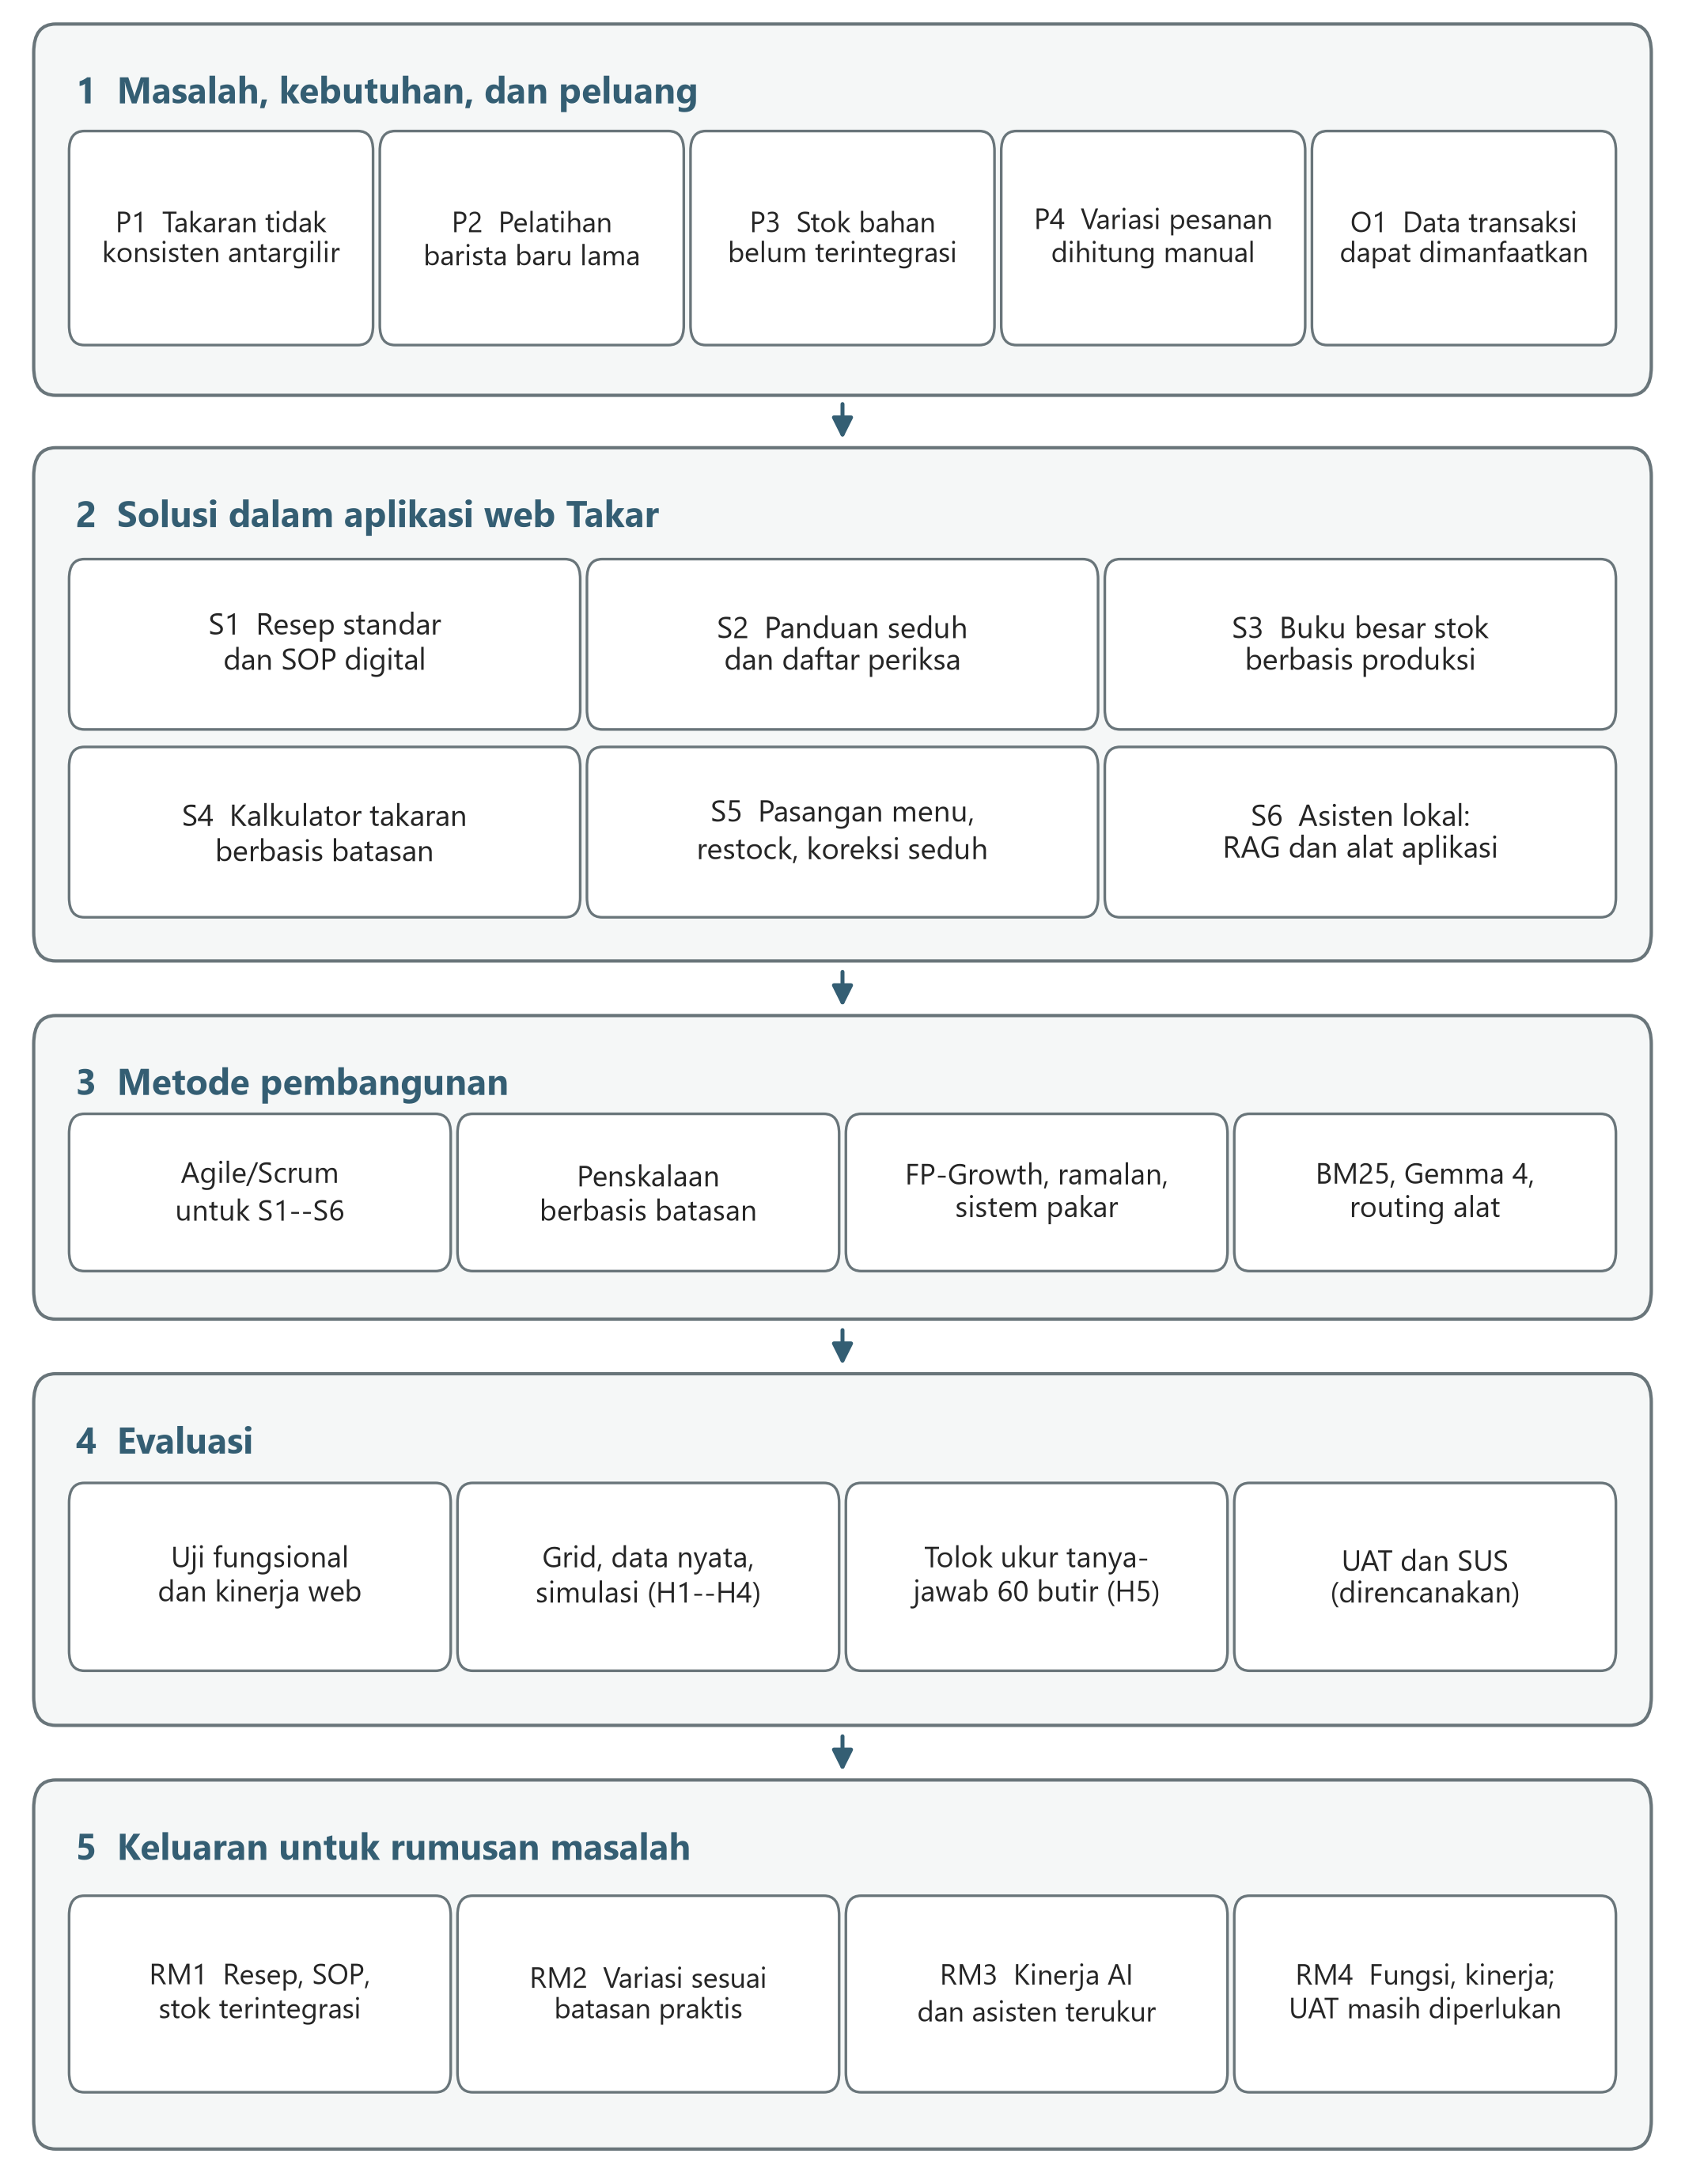
\includegraphics[width=\textwidth]{pic/kerangka_pemikiran.png}
\caption{Kerangka Pemikiran Penelitian}
\label{fig:kerangka-pemikiran}
\end{figure}

Lapis pertama memuat tiga masalah dari arahan, yaitu takaran resep yang tidak konsisten antar-\textit{shift} (P1), pelatihan barista baru yang memakan waktu lama (P2), dan inventaris bahan baku yang belum terintegrasi (P3); satu kebutuhan yang diturunkan penulis dari rumusan masalah arahan tentang kalkulator resep dinamis, yaitu kebutuhan bahan untuk variasi pesanan yang tanpa sistem harus dihitung manual (P4); serta satu peluang, yaitu data transaksi penjualan yang dapat diolah (O1). Lapis kedua memetakan masalah tersebut ke solusi pada aplikasi web Takar. Teori penyeduhan (Subbab~\ref{subsec:penyeduhan}) menunjukkan bahwa mutu seduhan dikendalikan oleh parameter yang dapat diukur, sehingga resep standar dan SOP digital (S1) dapat menjadi acuan yang sama bagi setiap \textit{shift}, sedangkan panduan seduh terpandu dan daftar periksa SOP (S2) berfungsi sebagai alat bantu kerja bagi barista baru (Subbab~\ref{subsec:kedai-kopi}). Buku besar stok yang terhubung ke produksi melalui BOM resep (S3) menjawab P3 (Subbab~\ref{subsec:persediaan}), dan kalkulator takaran dinamis (S4) menjawab P4 dengan penskalaan berbasis batasan karena faktor konversi linier dapat melanggar batasan bar (Subbab~\ref{subsec:penskalaan}). Modul AI operasional (S5) memanfaatkan O1 untuk rekomendasi pasangan menu dan \textit{restock}, serta bagan kendali seduh untuk koreksi parameter seduh. Asisten lokal (S6) membantu barista menemukan pengetahuan dalam resep dan SOP, serta menyerahkan perhitungan kepada layanan aplikasi (Subbab~\ref{subsec:llm-rag}).

Lapis ketiga memuat metode untuk membangun solusi tersebut, yaitu Scrum yang disesuaikan untuk S1--S6 (Subbab~\ref{subsec:scrum}), penskalaan berbasis batasan untuk S4, FP-Growth, peramalan dengan kebijakan persediaan, dan sistem pakar \textit{forward chaining} untuk S5 (Subbab~\ref{subsec:aturan-asosiasi}--\ref{subsec:sistem-pakar}), serta BM25, Gemma 4 lokal, dan pemanggilan alat untuk S6 (Subbab~\ref{subsec:llm-rag}). Lapis keempat memuat pengujian \textit{black-box}, evaluasi algoritma pada data sampel fiktif dan data nyata, tolok ukur tanya-jawab 60 butir untuk H5, pengukuran kinerja, serta UAT dengan SUS yang direncanakan. Lapis kelima memuat hasil untuk setiap rumusan masalah: resep, SOP, dan inventaris terintegrasi (RM1); takaran yang memenuhi batasan praktis (RM2); kinerja modul AI dan asisten yang terukur (RM3); serta pengujian fungsi dan kinerja dengan penerimaan pengguna yang masih perlu diperiksa (RM4).

Rantai argumen tersebut menurunkan lima hipotesis yang telah dirumuskan pada Subbab~\ref{sec:hipotesis}. H1 berasal dari teori penskalaan: algoritma berbasis batasan diharapkan menghindari pelanggaran praktis yang muncul dari penskalaan linier. H2 berasal dari teori aturan asosiasi: FP-Growth semestinya memberi HR@5 lebih tinggi daripada popularitas. H3 berasal dari teori peramalan: model yang dipilih pada data pengembangan semestinya memberi WAPE lebih rendah daripada naif musiman pada data uji. H4 berasal dari teori persediaan: kebijakan berbasis ramalan semestinya menghasilkan \textit{fill rate} lebih tinggi daripada ROP statis. H5 berasal dari teori RAG dan pemanggilan alat: asisten dengan keduanya diharapkan memberi akurasi jawaban lebih tinggi dan angka tanpa dasar lebih sedikit daripada model tanpa konteks pada pertanyaan yang sama. Kelima hipotesis dapat saja tidak didukung data, dan hasilnya dilaporkan apa adanya pada Bab~\ref{bab:hasil}.

% Kembalikan nilai \righthyphenmin untuk bab berikutnya.
\righthyphenmin=\babDuaRightHyphenMin\relax


% % Bab 3 : Metode Penelitian
\chapter{\babTiga}
\label{bab:metode}
% Sumber rancangan: app/SPEC.md, kode app/backend/app dan app/frontend/src,
% dataset/raw/*/DATASHEET.md, serta hasil terukur di app/results/.

\section{Desain Penelitian}
\label{sec:desain-penelitian}

Penelitian ini menggunakan pendekatan rancang bangun dan evaluasi komparatif. Artefak utamanya adalah Takar, aplikasi web untuk menyimpan resep dan prosedur operasional standar (SOP), menghitung variasi pesanan, mencatat pemakaian bahan, serta memberi rekomendasi operasional. Unit evaluasi ditetapkan sesuai keputusan yang didukung: satu pesanan untuk penskalaan resep, satu kueri keranjang untuk pasangan menu, satu pasangan produk--outlet--hari untuk peramalan, satu bahan--hari untuk simulasi persediaan, satu seduhan untuk sistem pakar, dan satu pertanyaan untuk asisten lokal. Pemisahan unit ini mencegah metrik dari tugas yang berbeda diperlakukan sebagai ukuran keberhasilan yang sama.

Rancangan dibagi menjadi analisis kebutuhan, pembuatan basis pengetahuan resep, implementasi aplikasi, pengujian fungsional, evaluasi algoritma, dan validasi eksternal. Data IBM dan Maven dipakai untuk pengembangan karena katalog produknya dapat dipetakan ke resep, tetapi keduanya merupakan data sampel fiktif. Oleh karena itu, penelitian ini juga menguji metode pada transaksi toko roti-kafe Edinburgh, penjualan mesin kopi ihelon, data seduhan konsumen UC Davis, resep eksperimen Batali, serta menu minuman Starbucks. Hasil pada sumber eksternal tidak dianggap sebagai bukti bahwa kinerja pada suatu kedai di Indonesia akan sama.

Arahan awal pembimbing menyebut Laravel dengan \textit{Progressive Web App}. Sesuai keputusan pengembangan tanggal 30 September 2026, implementasi memakai FastAPI (Python) dan Vue.js sebagai web responsif. Python dipilih agar pemrosesan data, pelatihan model, dan layanan API berada dalam lingkungan yang sama. Perubahan teknologi ini tidak mengubah masalah operasional, isi resep dari arahan, atau kebutuhan pencatatan inventaris.

\section{Tahapan Penelitian}
\label{sec:tahapan}

Tahapan penelitian mengikuti siklus analisis, perancangan, implementasi, pengujian, dan perbaikan bertahap. \textit{Product backlog} diturunkan dari tiga kendala utama arahan pembimbing: perbedaan takaran antarbarista, pelatihan staf baru, dan stok yang terpisah dari produksi. Kebutuhan variasi pesanan menjadi modul kalkulator; kebutuhan latihan menjadi panduan seduh dan checklist; kebutuhan stok menjadi buku besar pergerakan bahan. Modul AI menambah dukungan keputusan pasangan menu, peramalan dan pemesanan ulang, koreksi seduh, serta tanya-jawab berbasis pengetahuan lokal. Setiap iterasi menghasilkan fungsi yang bisa diuji melalui API dan antarmuka.

Gambar~\ref{fig:tahapan-penelitian} menunjukkan bahwa temuan pengujian dikembalikan ke rancangan. Urutan tersebut penting karena resep dan satuan bahan harus benar sebelum hasil penskalaan dipakai untuk memotong stok atau mengubah ramalan produk menjadi kebutuhan bahan. Setiap berkas hasil evaluasi menyimpan parameter, cap waktu, serta identitas data sehingga hasil pada Bab~\ref{bab:hasil} dapat ditelusuri ke prosedur pembuatnya.

\begin{figure}[htbp]
\centering
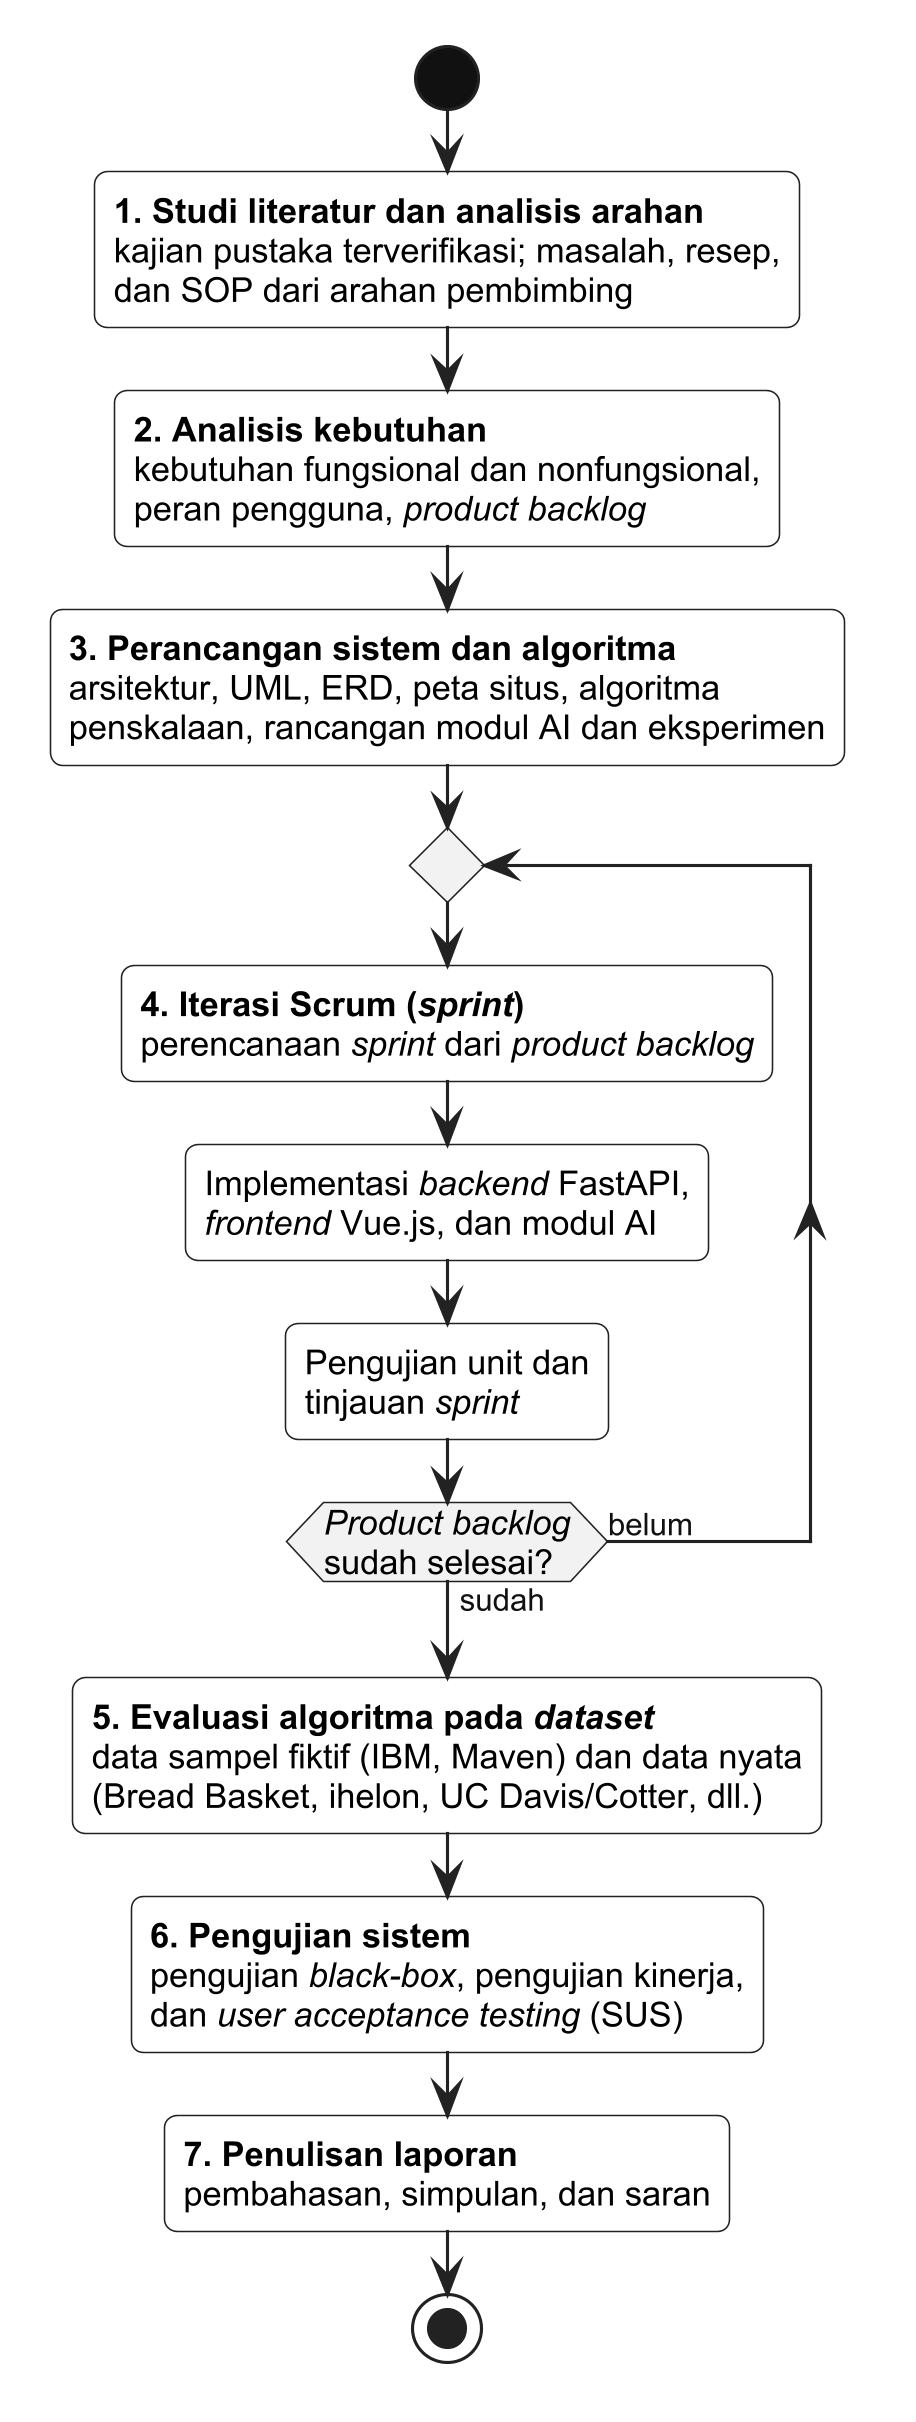
\includegraphics[width=.58\textwidth]{pic/tahapan_penelitian.png}
\caption{Tahapan Penelitian dan Umpan Balik Pengujian}
\label{fig:tahapan-penelitian}
\end{figure}

\section{Analisis Kebutuhan}
\label{sec:analisis-kebutuhan}

Pengguna dibagi menjadi manajer, kepala barista, dan barista. Ketiganya dapat melihat resep, SOP, kalkulator, panduan seduh, serta rekomendasi; dapat pula mencatat produksi dan mengerjakan checklist. Manajer dan kepala barista dapat mengubah resep, SOP, dan bahan serta mencatat penerimaan, penyesuaian, dan bahan terbuang. Hanya manajer dapat mengelola akun, menonaktifkan resep, dan melatih ulang model. Pemeriksaan hak akses dilakukan kembali di server, tidak hanya dengan menyembunyikan tombol di antarmuka.

Kebutuhan fungsional pertama adalah menyimpan resep dalam ukuran dasar beserta komponen, satuan, aturan penskalaan, parameter mutu, dan langkah pembuatan. Kebutuhan kedua adalah menghasilkan takaran per cangkir dan total pesanan untuk ukuran, jumlah cangkir, sajian panas atau dingin, tingkat manis, tambahan \textit{shot}, penggantian susu atau biji, dan dosis V60. Kebutuhan ketiga adalah menghubungkan produksi yang dicatat dengan pergerakan stok bahan secara atomik dan menjaga agar permintaan yang dikirim ulang tidak memotong stok dua kali. Kebutuhan keempat adalah menyajikan SOP, timer, ilustrasi tindakan yang mengikuti tahap resep, riwayat produksi, status bahan, dan penjelasan rekomendasi pada antarmuka berbahasa Indonesia. Saran pasangan menu yang memiliki padanan resep aktif harus dapat dibuka langsung sebagai panduan seduh.

Kebutuhan nonfungsional mencakup tampilan yang dapat digunakan pada tablet dan ponsel, validasi masukan di server, autentikasi JWT, kata sandi yang di-\textit{hash} dengan Argon2, pembatasan percobaan masuk, dan keluaran AI yang menyatakan sumber serta batasnya. Sistem ditujukan bagi satu outlet dengan basis data SQLite. Integrasi kasir, pesanan pembelian, multi-outlet, dan operasi luring berada di luar ruang lingkup. Angka stok awal, kemasan, harga, dan \textit{lead time} yang tidak tercantum dalam arahan adalah data contoh yang dicatat di \texttt{app/backend/app/seed/ASSUMPTIONS.md}.

\section{Perancangan Sistem}
\label{sec:perancangan-sistem}

Arsitektur pada Gambar~\ref{fig:arsitektur} memisahkan antarmuka Vue.js, API FastAPI, basis data SQLite, dan proses pelatihan atau evaluasi yang dijalankan sebagai skrip. Antarmuka mengirim permintaan JSON dengan token pengguna. API menerapkan autentikasi, validasi, logika resep dan stok, lalu membaca hasil model yang telah disimpan. Proses eksperimen membaca berkas data mentah dan menulis hasil JSON/CSV ke direktori \texttt{app/results}; berkas hasil tidak diisi manual. Pada mode satu port, FastAPI juga menyajikan hasil \textit{build} antarmuka.

\begin{figure}[htbp]
\centering
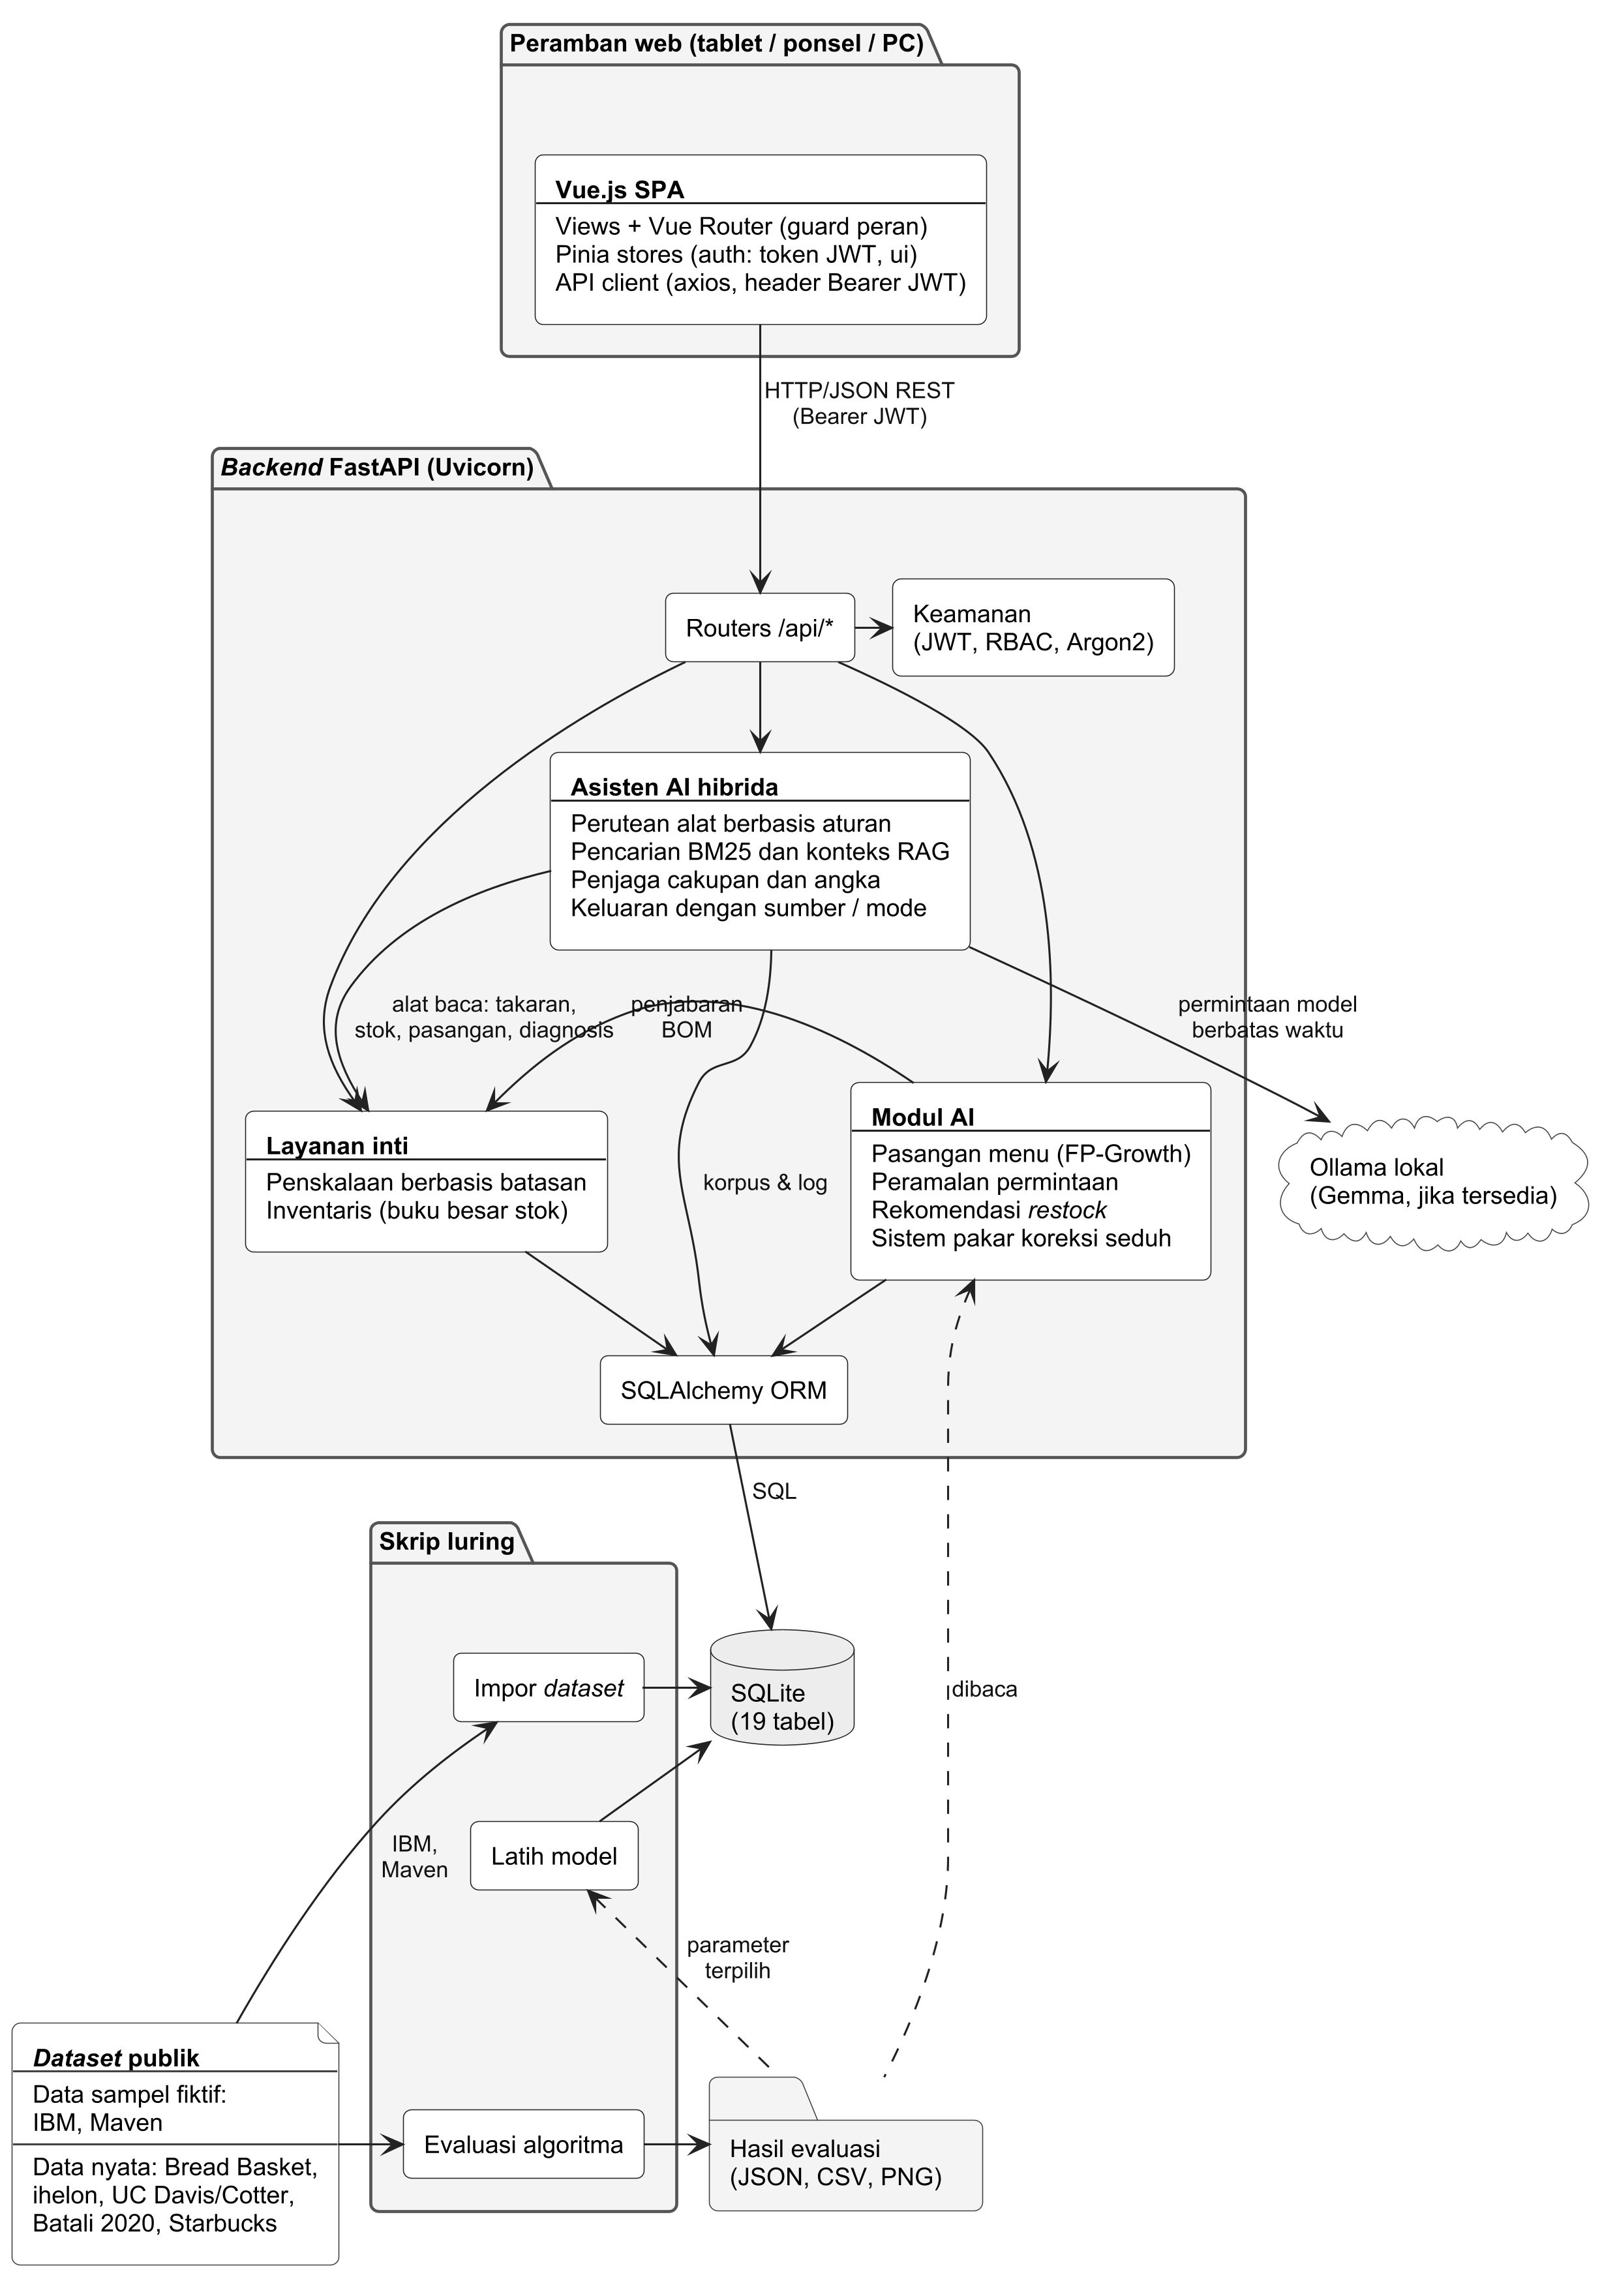
\includegraphics[width=.92\textwidth]{pic/arsitektur.png}
\caption{Arsitektur Aplikasi Takar}
\label{fig:arsitektur}
\end{figure}

Hubungan aktor dengan fungsi utama ditunjukkan pada Gambar~\ref{fig:use-case}. Alur kalkulator pada Gambar~\ref{fig:activity-kalkulator} berakhir pada pratinjau kebutuhan bahan dan peringatan; pengguna masih harus memilih tindakan catat produksi. Sesudah dicatat, setiap komponen resep turunan diuraikan menjadi bahan dasar dan ditulis sebagai pergerakan stok. Diagram sekuens pada Gambar~\ref{fig:sequence-produce} memperlihatkan bahwa perhitungan, log produksi, dan mutasi stok berada di sisi server sehingga tampilan yang ditutup tidak mengubah konsistensi catatan.

\begin{figure}[htbp]
\centering
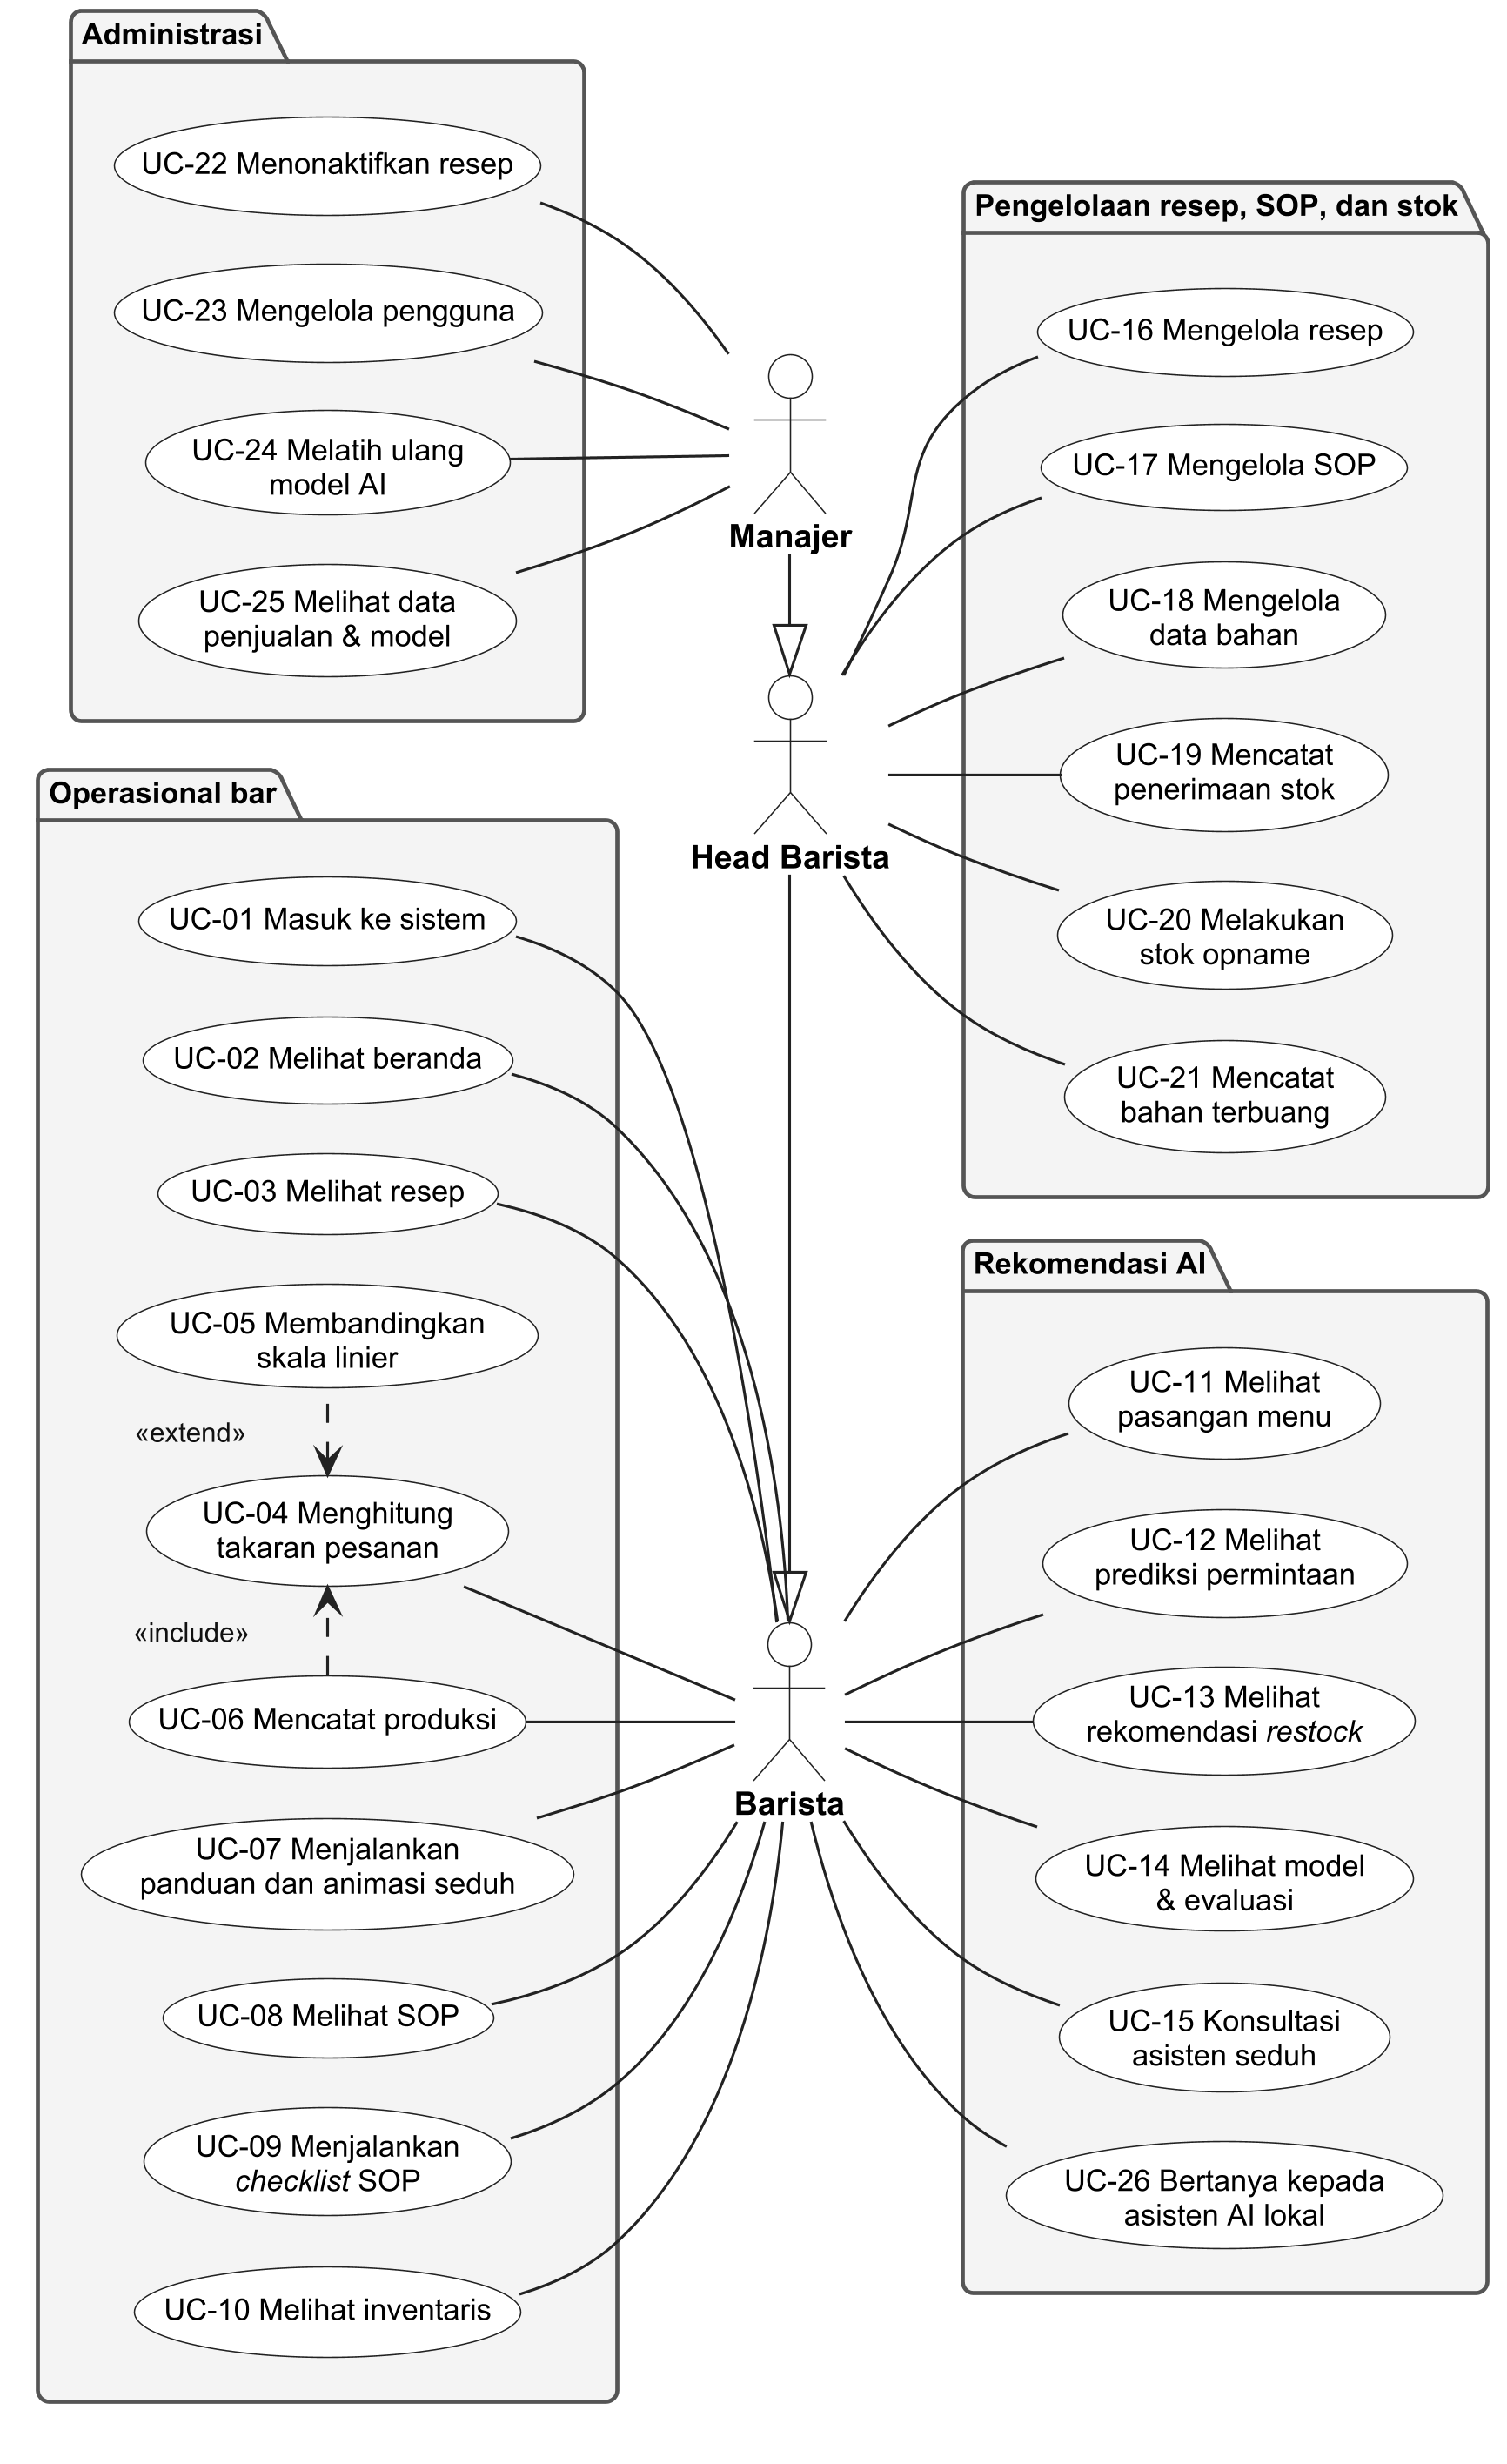
\includegraphics[width=.85\textwidth]{pic/use_case.png}
\caption{Kasus Penggunaan Menurut Peran}
\label{fig:use-case}
\end{figure}
\begin{figure}[htbp]
\centering
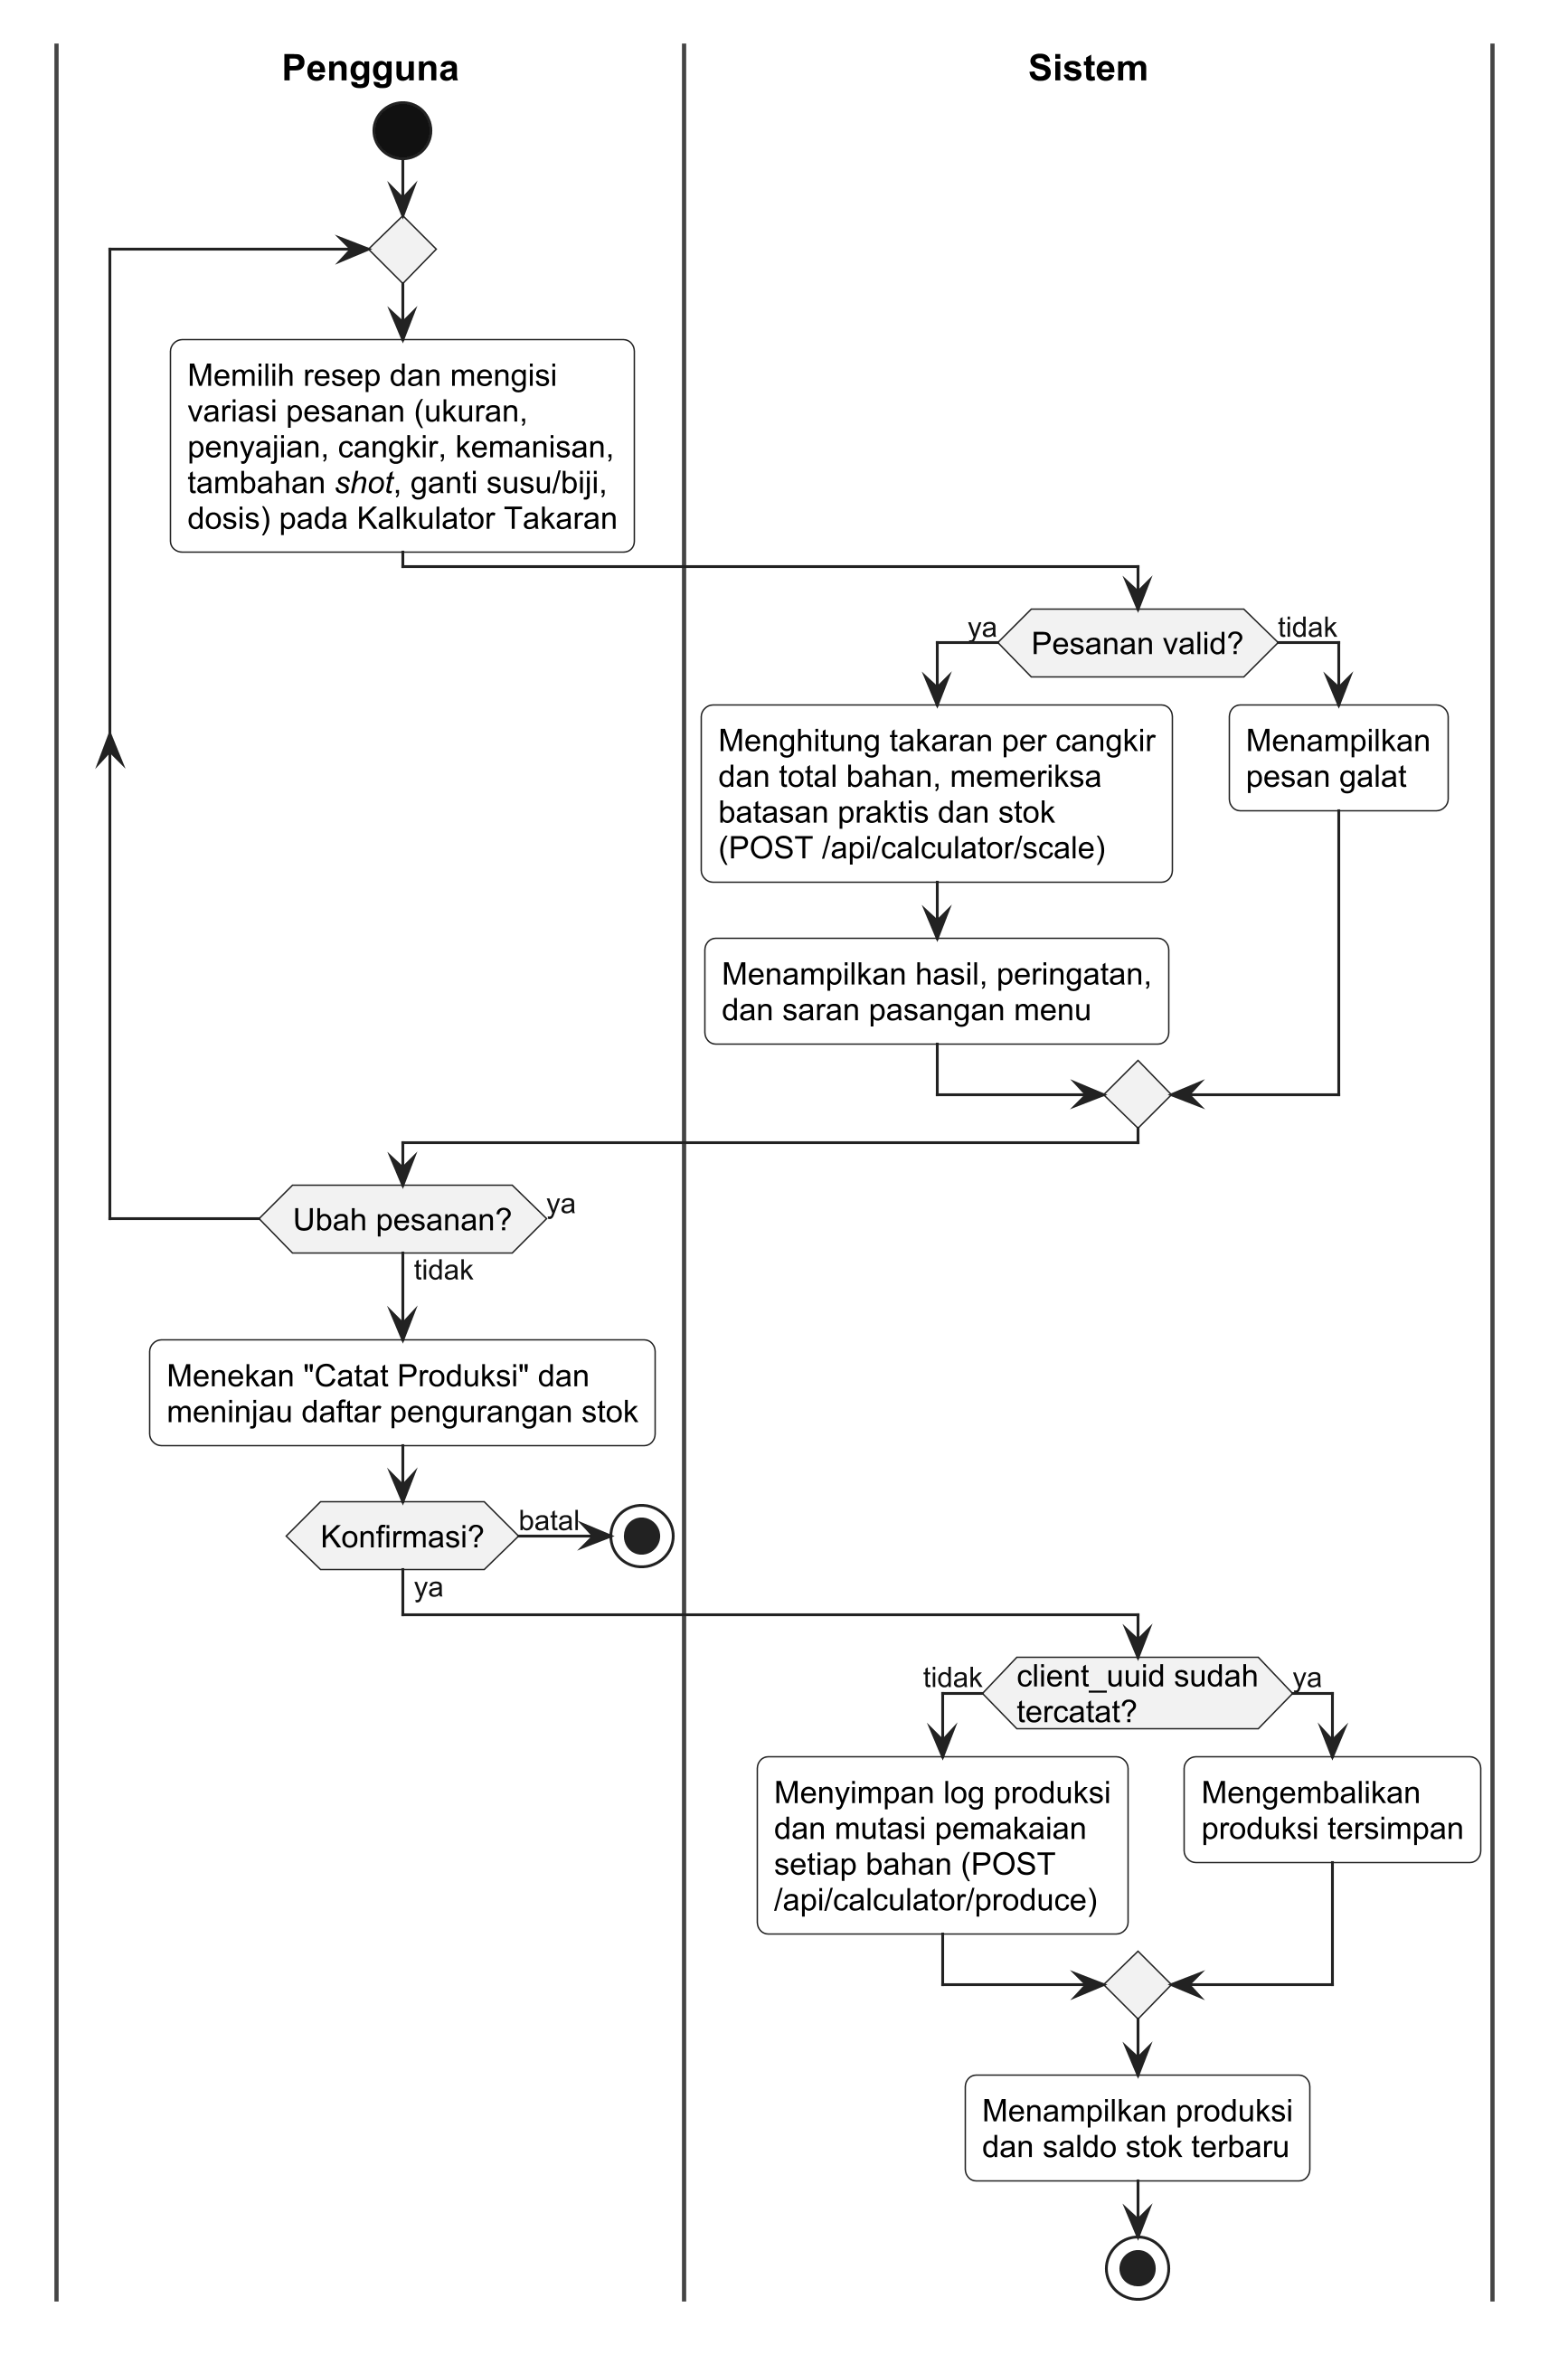
\includegraphics[width=.75\textwidth]{pic/activity_kalkulator.png}
\caption{Aktivitas Perhitungan Variasi Pesanan}
\label{fig:activity-kalkulator}
\end{figure}
\begin{figure}[htbp]
\centering
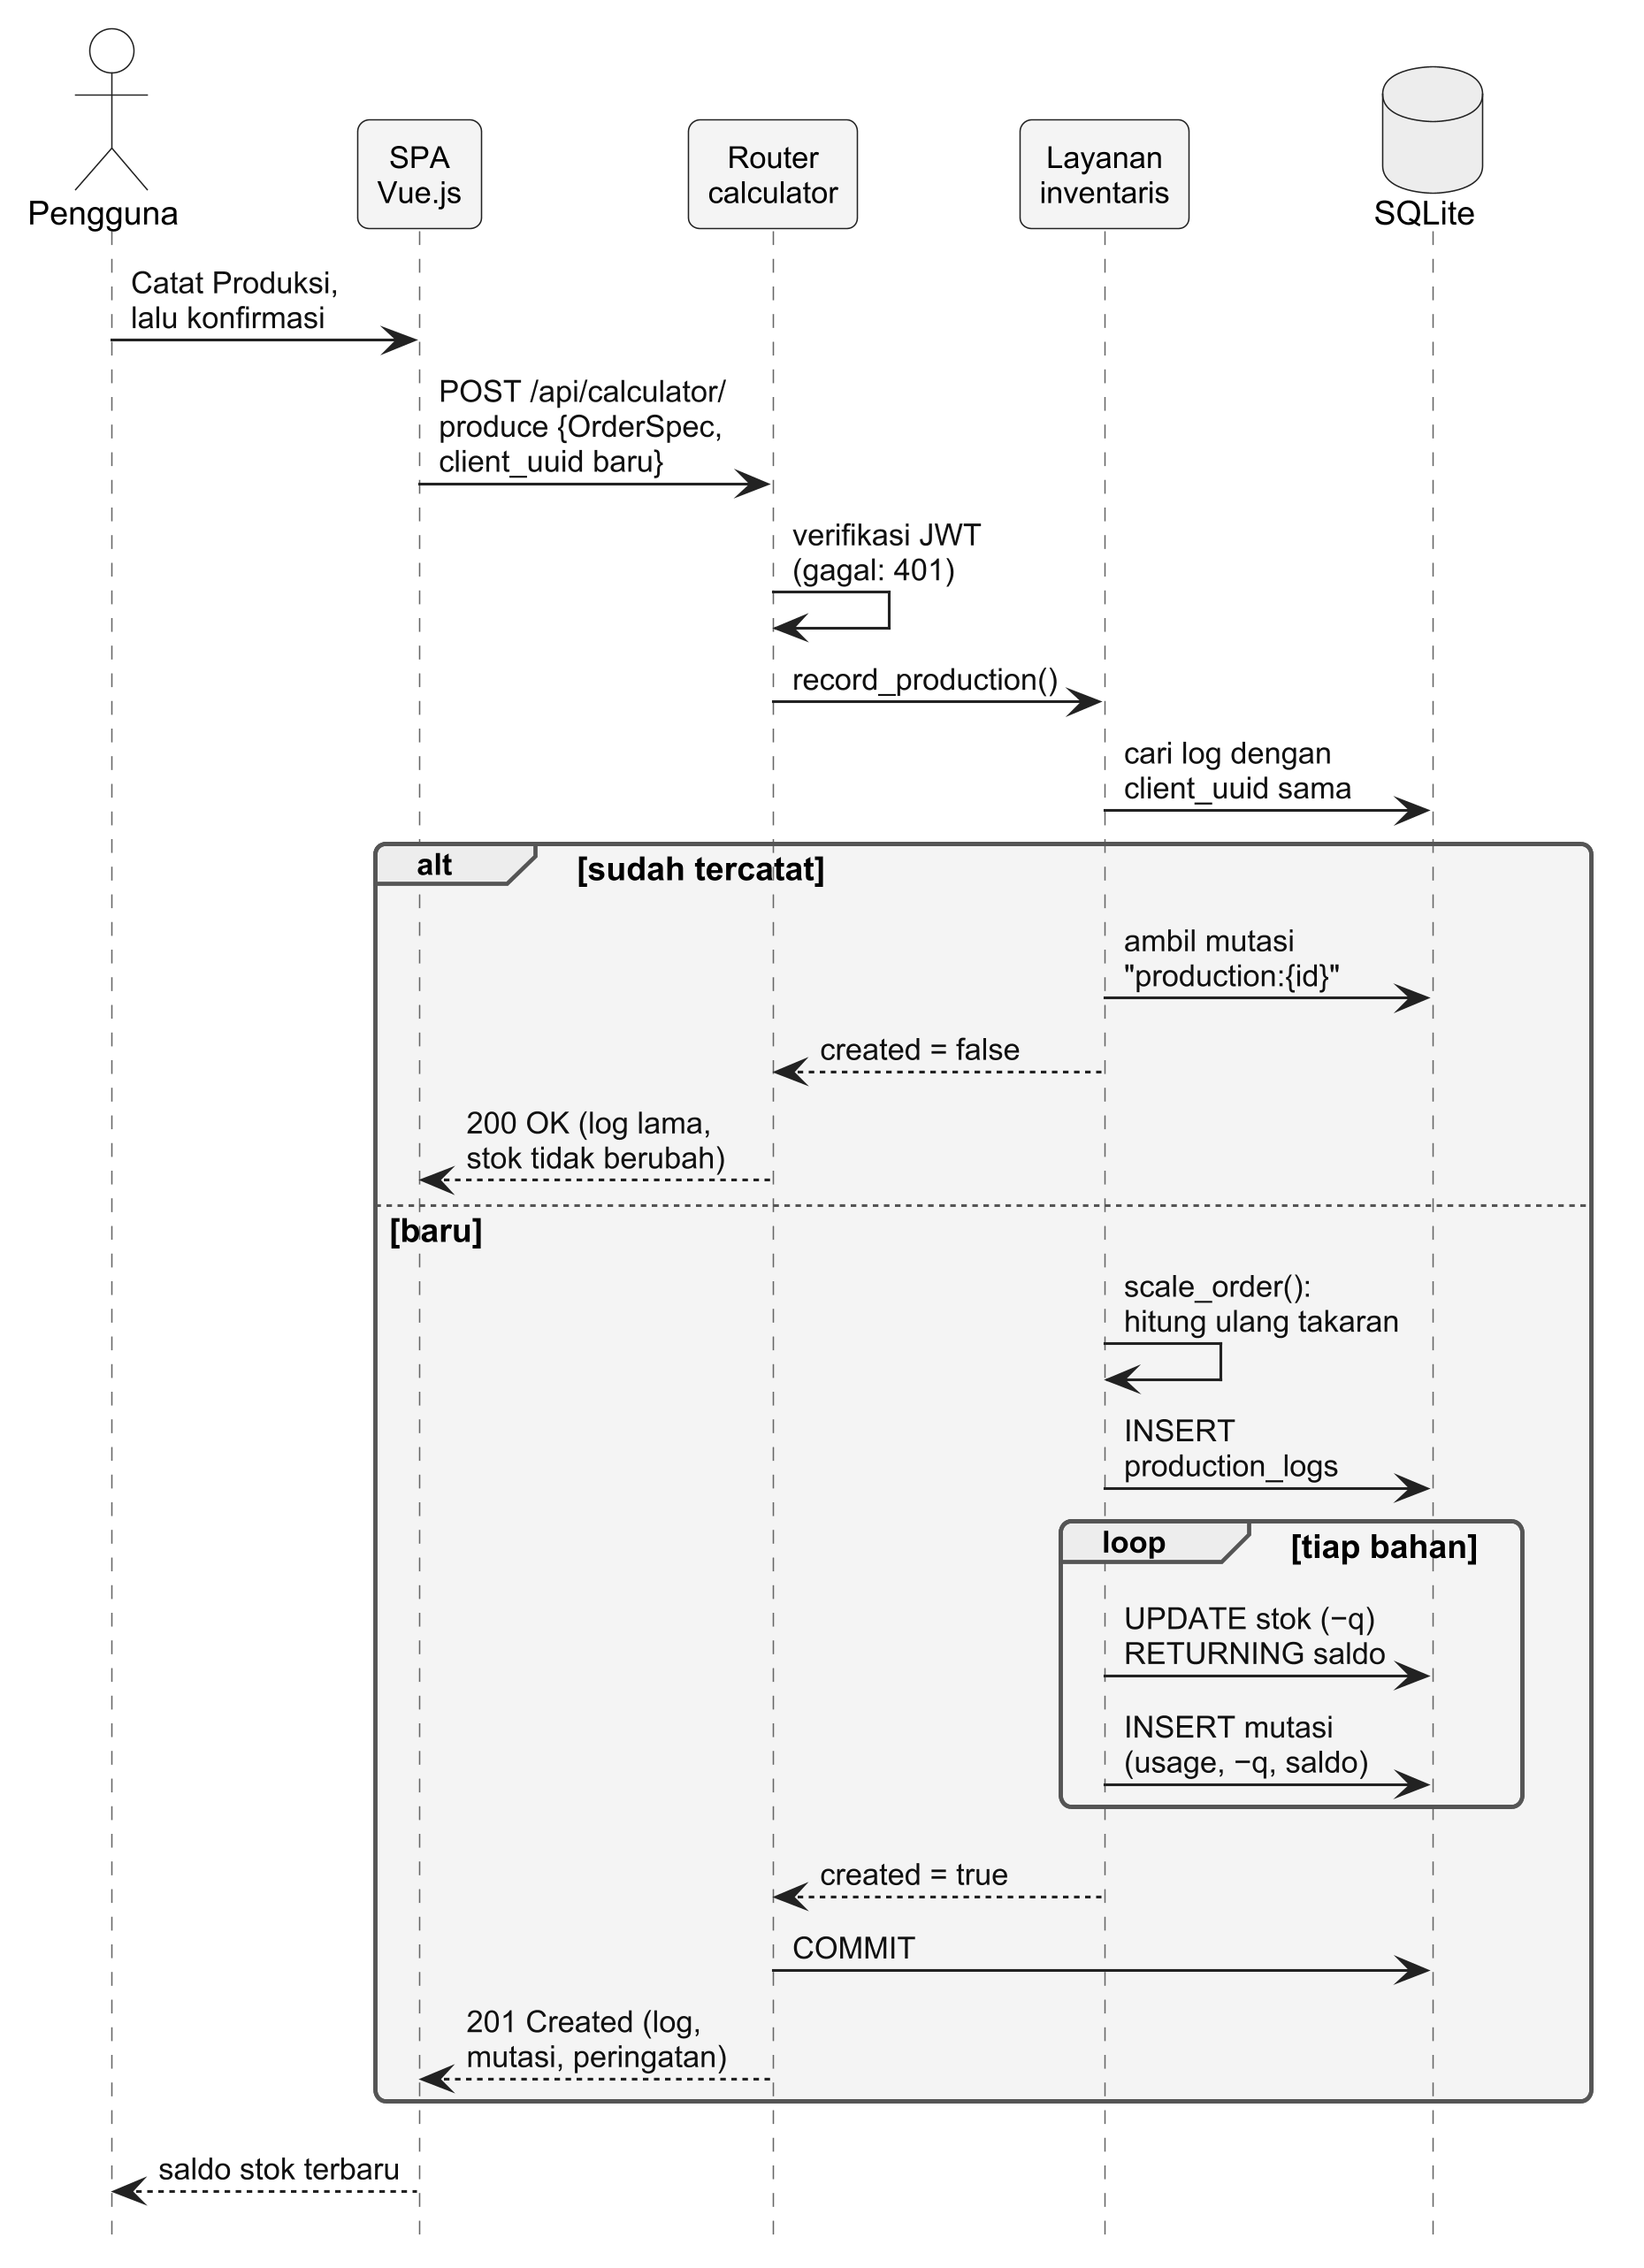
\includegraphics[width=.84\textwidth]{pic/sequence_produce.png}
\caption{Sekuens Pencatatan Produksi dan Pergerakan Stok}
\label{fig:sequence-produce}
\end{figure}

Rancangan data pada Gambar~\ref{fig:erd} menggunakan resep dan komponen sebagai daftar bahan (\textit{bill of materials}, BOM). Komponen dapat menunjuk bahan langsung atau subresep, misalnya satu \textit{shot} espreso yang memiliki kebutuhan biji sendiri. Ukuran resep menyimpan volume cangkir dan pengecualian jumlah \textit{shot} per ukuran. Tabel pergerakan inventaris menyimpan kuantitas bertanda dan saldo setelah transaksi; stok bahan berubah hanya lewat layanan pencatatan pergerakan. Tabel penjualan, aturan pasangan, prakiraan, dan riwayat pelatihan mendukung model AI tanpa menggabungkan transaksi dataset publik dengan produksi kedai demo. Log asisten menyimpan pertanyaan, jawaban, mode, rujukan, alat yang digunakan, dan latensi untuk penelusuran kesalahan pada instalasi lokal.

\begin{figure}[htbp]
\centering
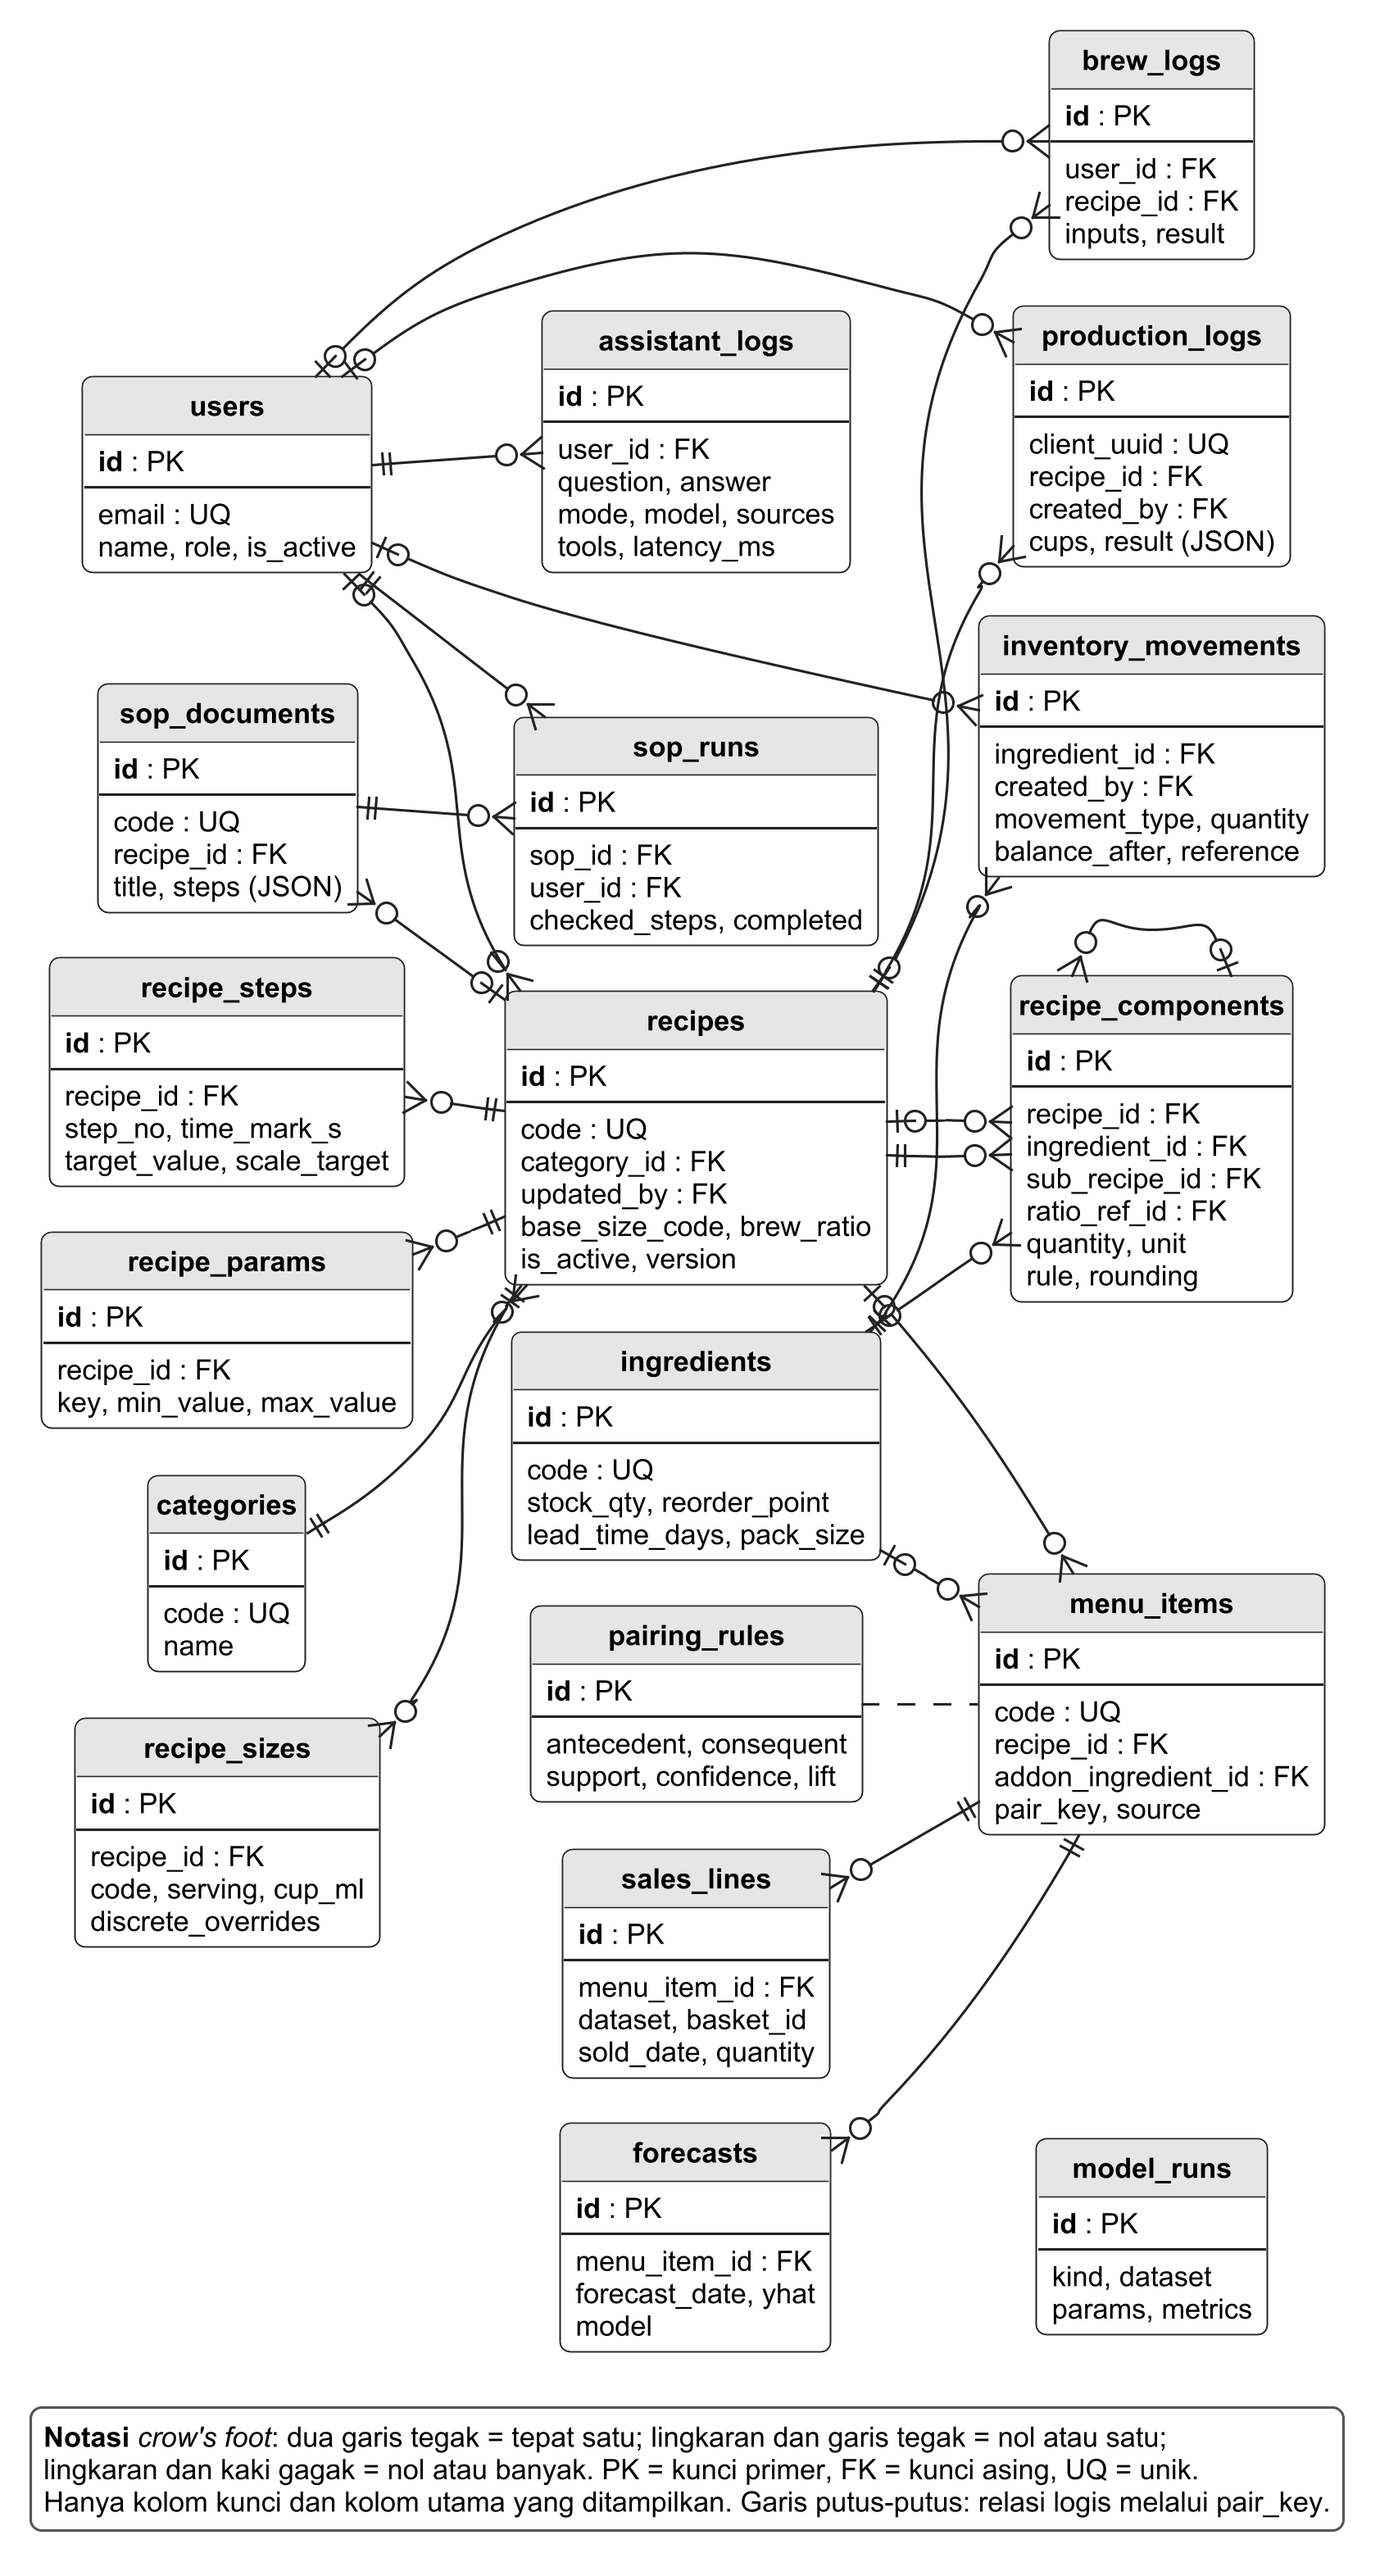
\includegraphics[width=.86\textwidth]{pic/erd.png}
\caption{Rancangan Entitas dan Relasi Basis Data Takar}
\label{fig:erd}
\end{figure}

Kontrak layanan utama dirangkum pada Tabel~\ref{tab:endpoint}. Seluruh alamat pada tabel memakai awalan \texttt{/api}. Permintaan tanpa token atau dengan peran yang tidak berhak dikembalikan sebagai HTTP 401 atau 403; masukan yang tidak memenuhi aturan dikembalikan sebagai HTTP 422. Pencatatan produksi memakai pengenal permintaan klien untuk mencegah pengurangan stok berulang akibat pengiriman ulang.

\begin{table}[htbp]
\centering
\caption{Kelompok \textit{Endpoint} API Utama}
\label{tab:endpoint}
\begin{tabular}{p{.27\textwidth}p{.59\textwidth}}
\toprule
Kelompok & Fungsi \\
\midrule
\texttt{/auth}, \texttt{/users} & Masuk, identitas sesi, dan pengelolaan pengguna. \\
\texttt{/recipes}, \texttt{/sop} & Katalog, detail, perubahan resep dan SOP, serta checklist. \\
\texttt{/calculator} & Penskalaan, pembanding linier, produksi, dan riwayat. \\
\texttt{/ingredients}, \texttt{/inventory} & Data bahan, stok, penerimaan, penyesuaian, limbah, dan buku besar. \\
\texttt{/ai}, \texttt{/sales} & Pasangan menu, peramalan, \textit{restock}, diagnosis seduh, model, dan ringkasan transaksi. \\
\texttt{/dashboard}, \texttt{/assistant} & Ringkasan operasional dan layanan asisten tanya-jawab lokal. \\
\bottomrule
\end{tabular}
\end{table}

Peta navigasi pada Gambar~\ref{fig:peta-situs} menempatkan kalkulator dan panduan seduh dekat detail resep agar barista dapat beralih dari membaca standar ke menjalankannya. Menu manajemen resep, inventaris, data model, dan pengguna mengikuti hak akses. Komponen tampilan menyajikan status kosong dan kesalahan secara jelas, termasuk saat model belum dilatih atau layanan model bahasa lokal tidak tersedia.

\begin{figure}[htbp]
\centering
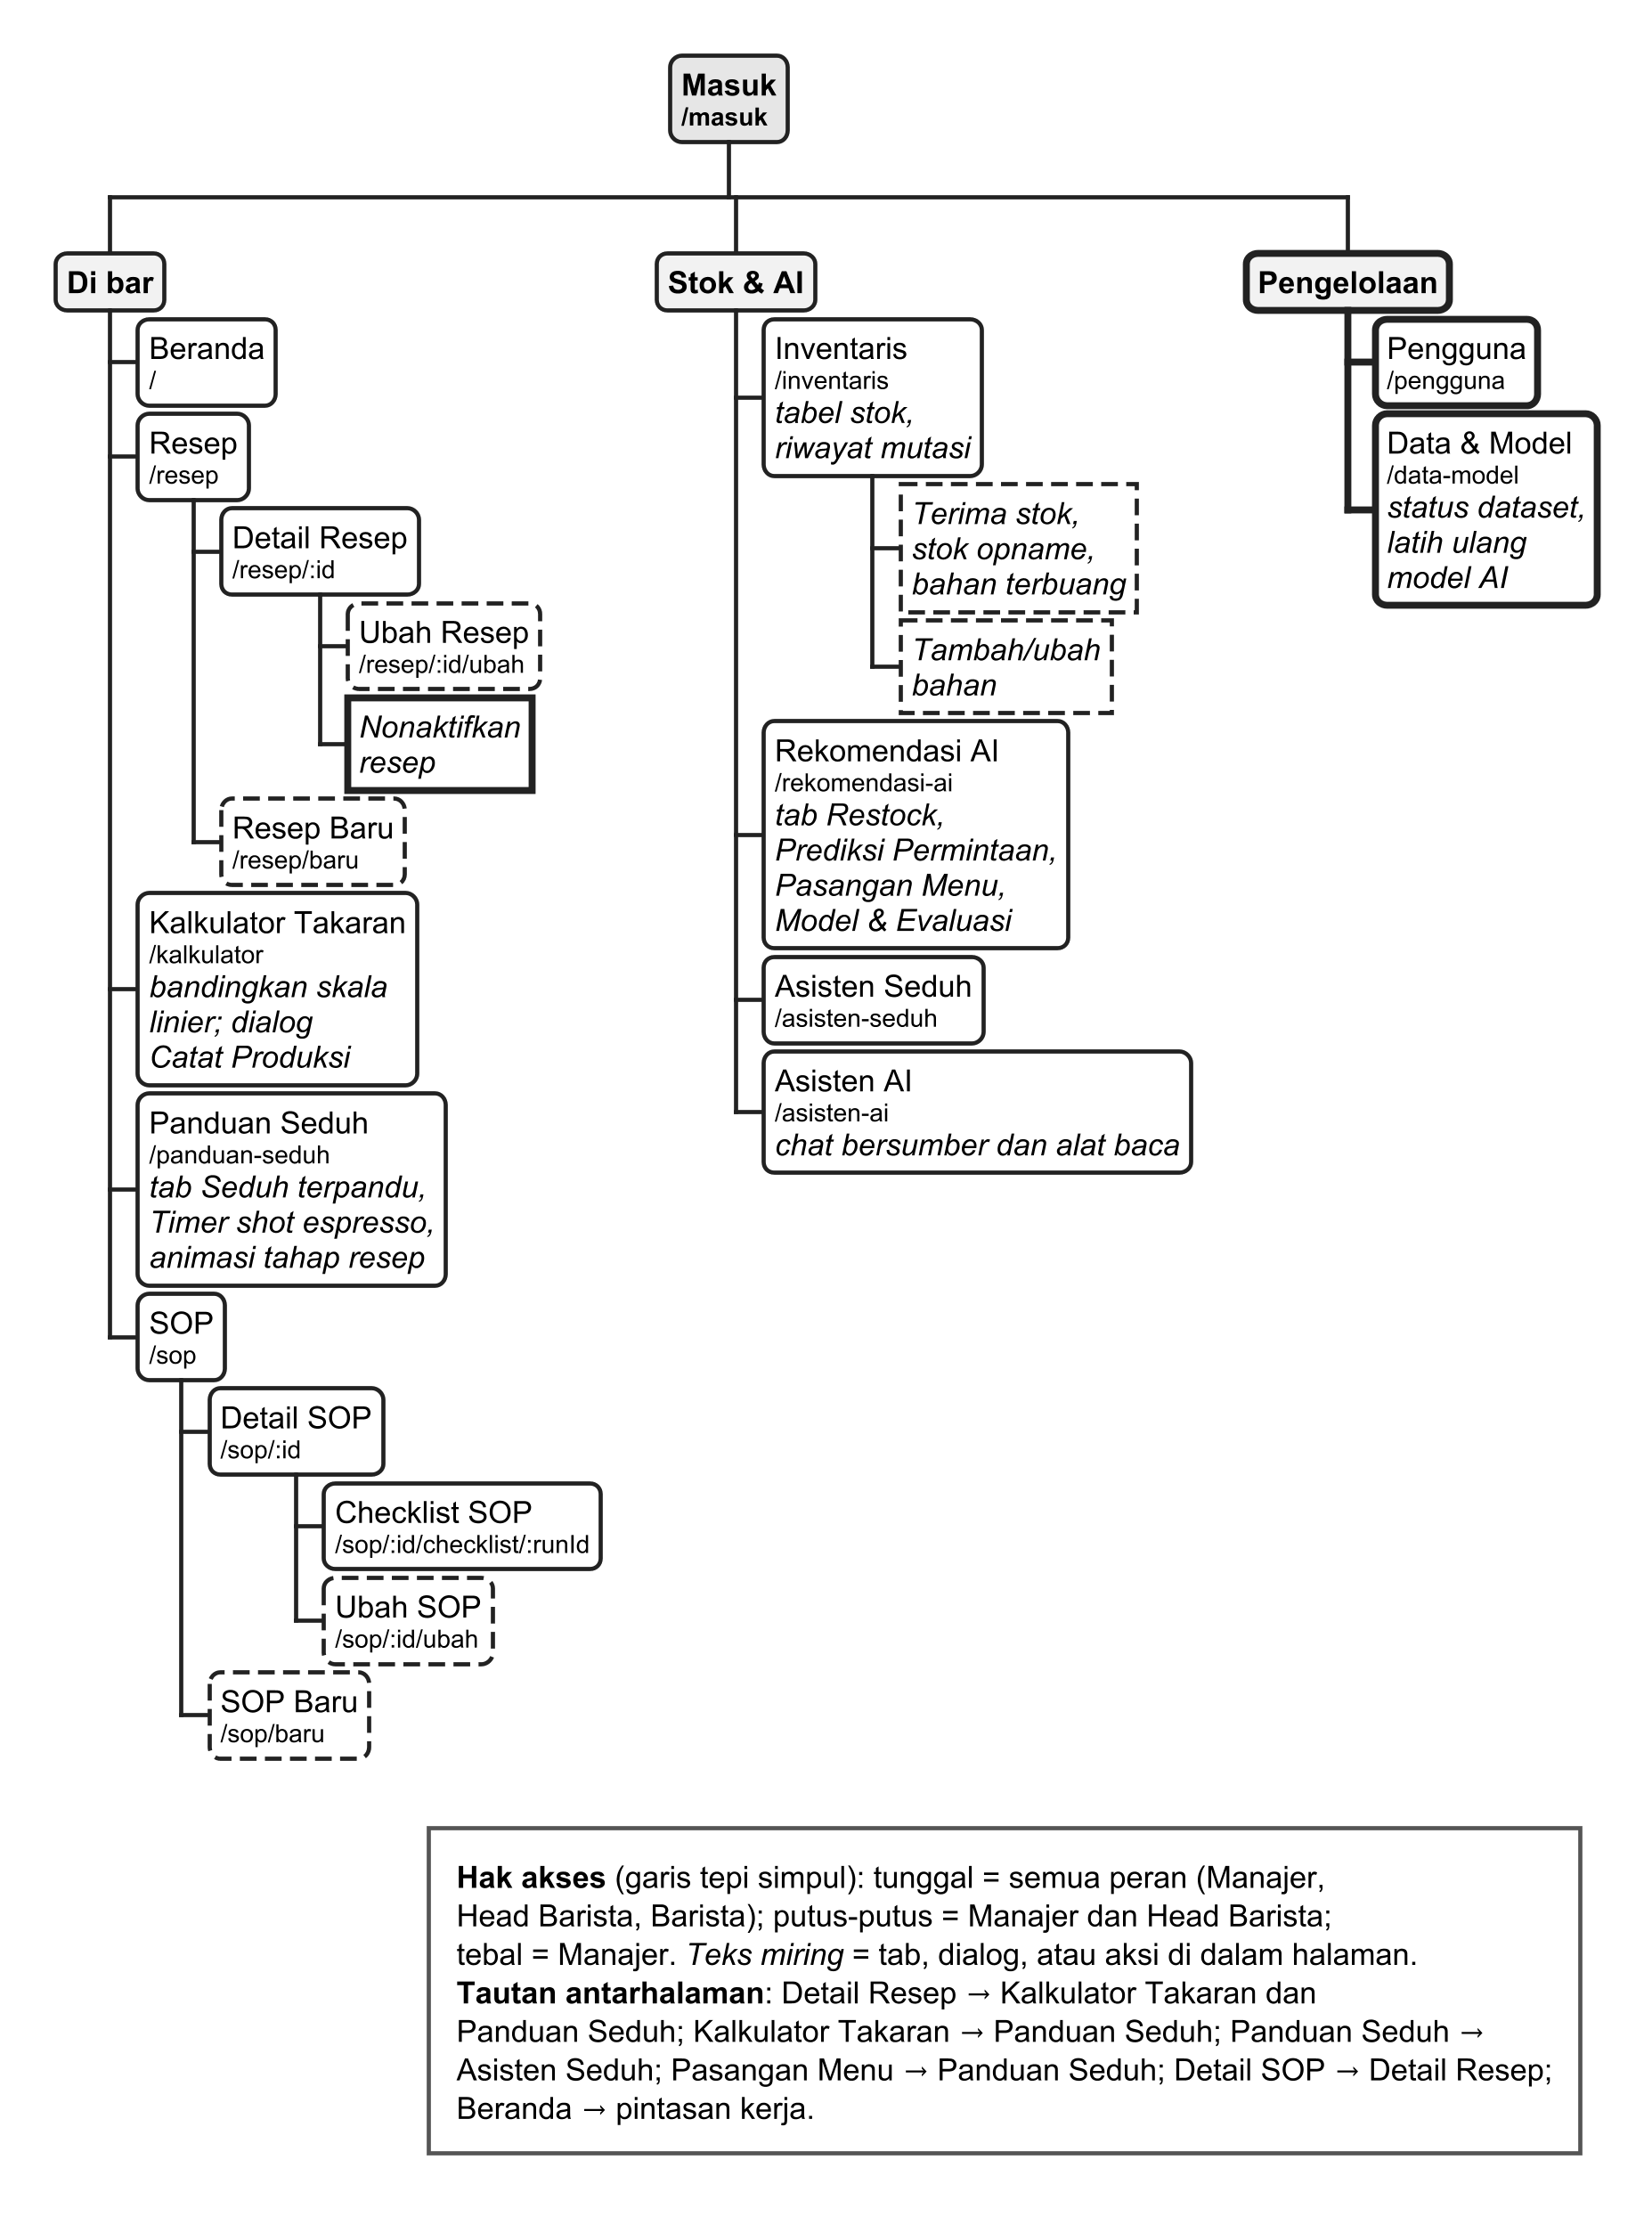
\includegraphics[width=.85\textwidth]{pic/peta_situs.png}
\caption{Peta Navigasi Aplikasi}
\label{fig:peta-situs}
\end{figure}

\section{Perancangan Algoritma}
\label{sec:perancangan-algoritma}

\subsection{Penskalaan Resep Berbasis Batasan}

Setiap resep memiliki ukuran dasar dan aturan untuk setiap komponen. Untuk ukuran yang dipilih, faktor awal adalah volume cangkir yang diminta dibagi volume dasar. Pada V60, dosis yang diminta mengganti faktor tersebut dengan rasio dosis baru terhadap dosis dasar. Komponen proporsional dikalikan faktor; komponen tetap tidak berubah; \textit{shot} dibulatkan ke kelipatan utuh atau mengikuti tabel pengecualian ukuran. Pemanis mengikuti persentase manis. Air dengan aturan rasio dihitung sesudah dosis akhir diketahui, sedangkan susu pengisi dihitung setelah volume komponen lain agar tidak melampaui cangkir.

Algoritma~\ref{alg:penskalaan} menyatakan urutan ketergantungan tersebut. Pembulatan mengikuti ketelitian takar masing-masing bahan. Target tuang kumulatif V60 ikut diskalakan, sedangkan waktu penanda langkah tetap. Jika es dan bahan lain sudah memenuhi cangkir, jumlah es dapat dikurangi; pesanan dengan komponen pengisi yang tetap melampaui batas ditolak. Subresep kemudian diuraikan menjadi bahan dasar per cangkir dan dikalikan jumlah cangkir, sehingga jumlah total tepat merupakan kelipatan takaran per cangkir. Pemeriksaan menghasilkan peringatan untuk luapan, kurang isi, perubahan rasio, dosis di luar rentang, dan stok yang kurang.

\begin{algorithm}[htbp]
\caption{Penskalaan Resep Berbasis Batasan}
\label{alg:penskalaan}
\begin{algorithmic}[1]
\Require resep, ukuran, sajian, jumlah cangkir, manis, \textit{shot}, pertukaran bahan, dosis
\Ensure takaran per cangkir, kebutuhan total, langkah, dan peringatan
\State Tentukan volume cangkir dan faktor ukuran atau faktor dosis
\State Pilih komponen sajian; terapkan pertukaran yang sah
\For{setiap komponen proporsional, tetap, dan diskret}
  \State Hitung menurut aturan; terapkan manis dan tambahan \textit{shot}
  \State Bulatkan ke ketelitian takar komponen
\EndFor
\For{setiap komponen rasio}
  \State Hitung dari komponen acuan yang sudah final
\EndFor
\State Hitung ruang setelah volume bahan lain dan es diperiksa
\State Isi komponen \textit{top up}; tolak pesanan yang tidak muat
\State Skala target langkah dan periksa seluruh batasan
\State Uraikan subresep menjadi bahan dasar per cangkir
\State Kalikan kebutuhan per cangkir dengan jumlah cangkir
\State \Return hasil dan peringatan
\end{algorithmic}
\end{algorithm}

Gambar~\ref{fig:alur-penskalaan} merinci cabang aturan untuk komponen yang berbeda. Pembanding pertama adalah penskalaan linier mentah yang mengalikan semua kuantitas dasar dengan faktor. Pembanding kedua membulatkan hasil linier ke ketelitian takar, termasuk \textit{shot}, tetapi tidak memperhitungkan pengisian dan ruang cangkir. Pembanding kedua memisahkan efek pembulatan dari efek aturan kapasitas. Ketiganya dinilai pada pesanan yang setara.

\begin{figure}[htbp]
\centering
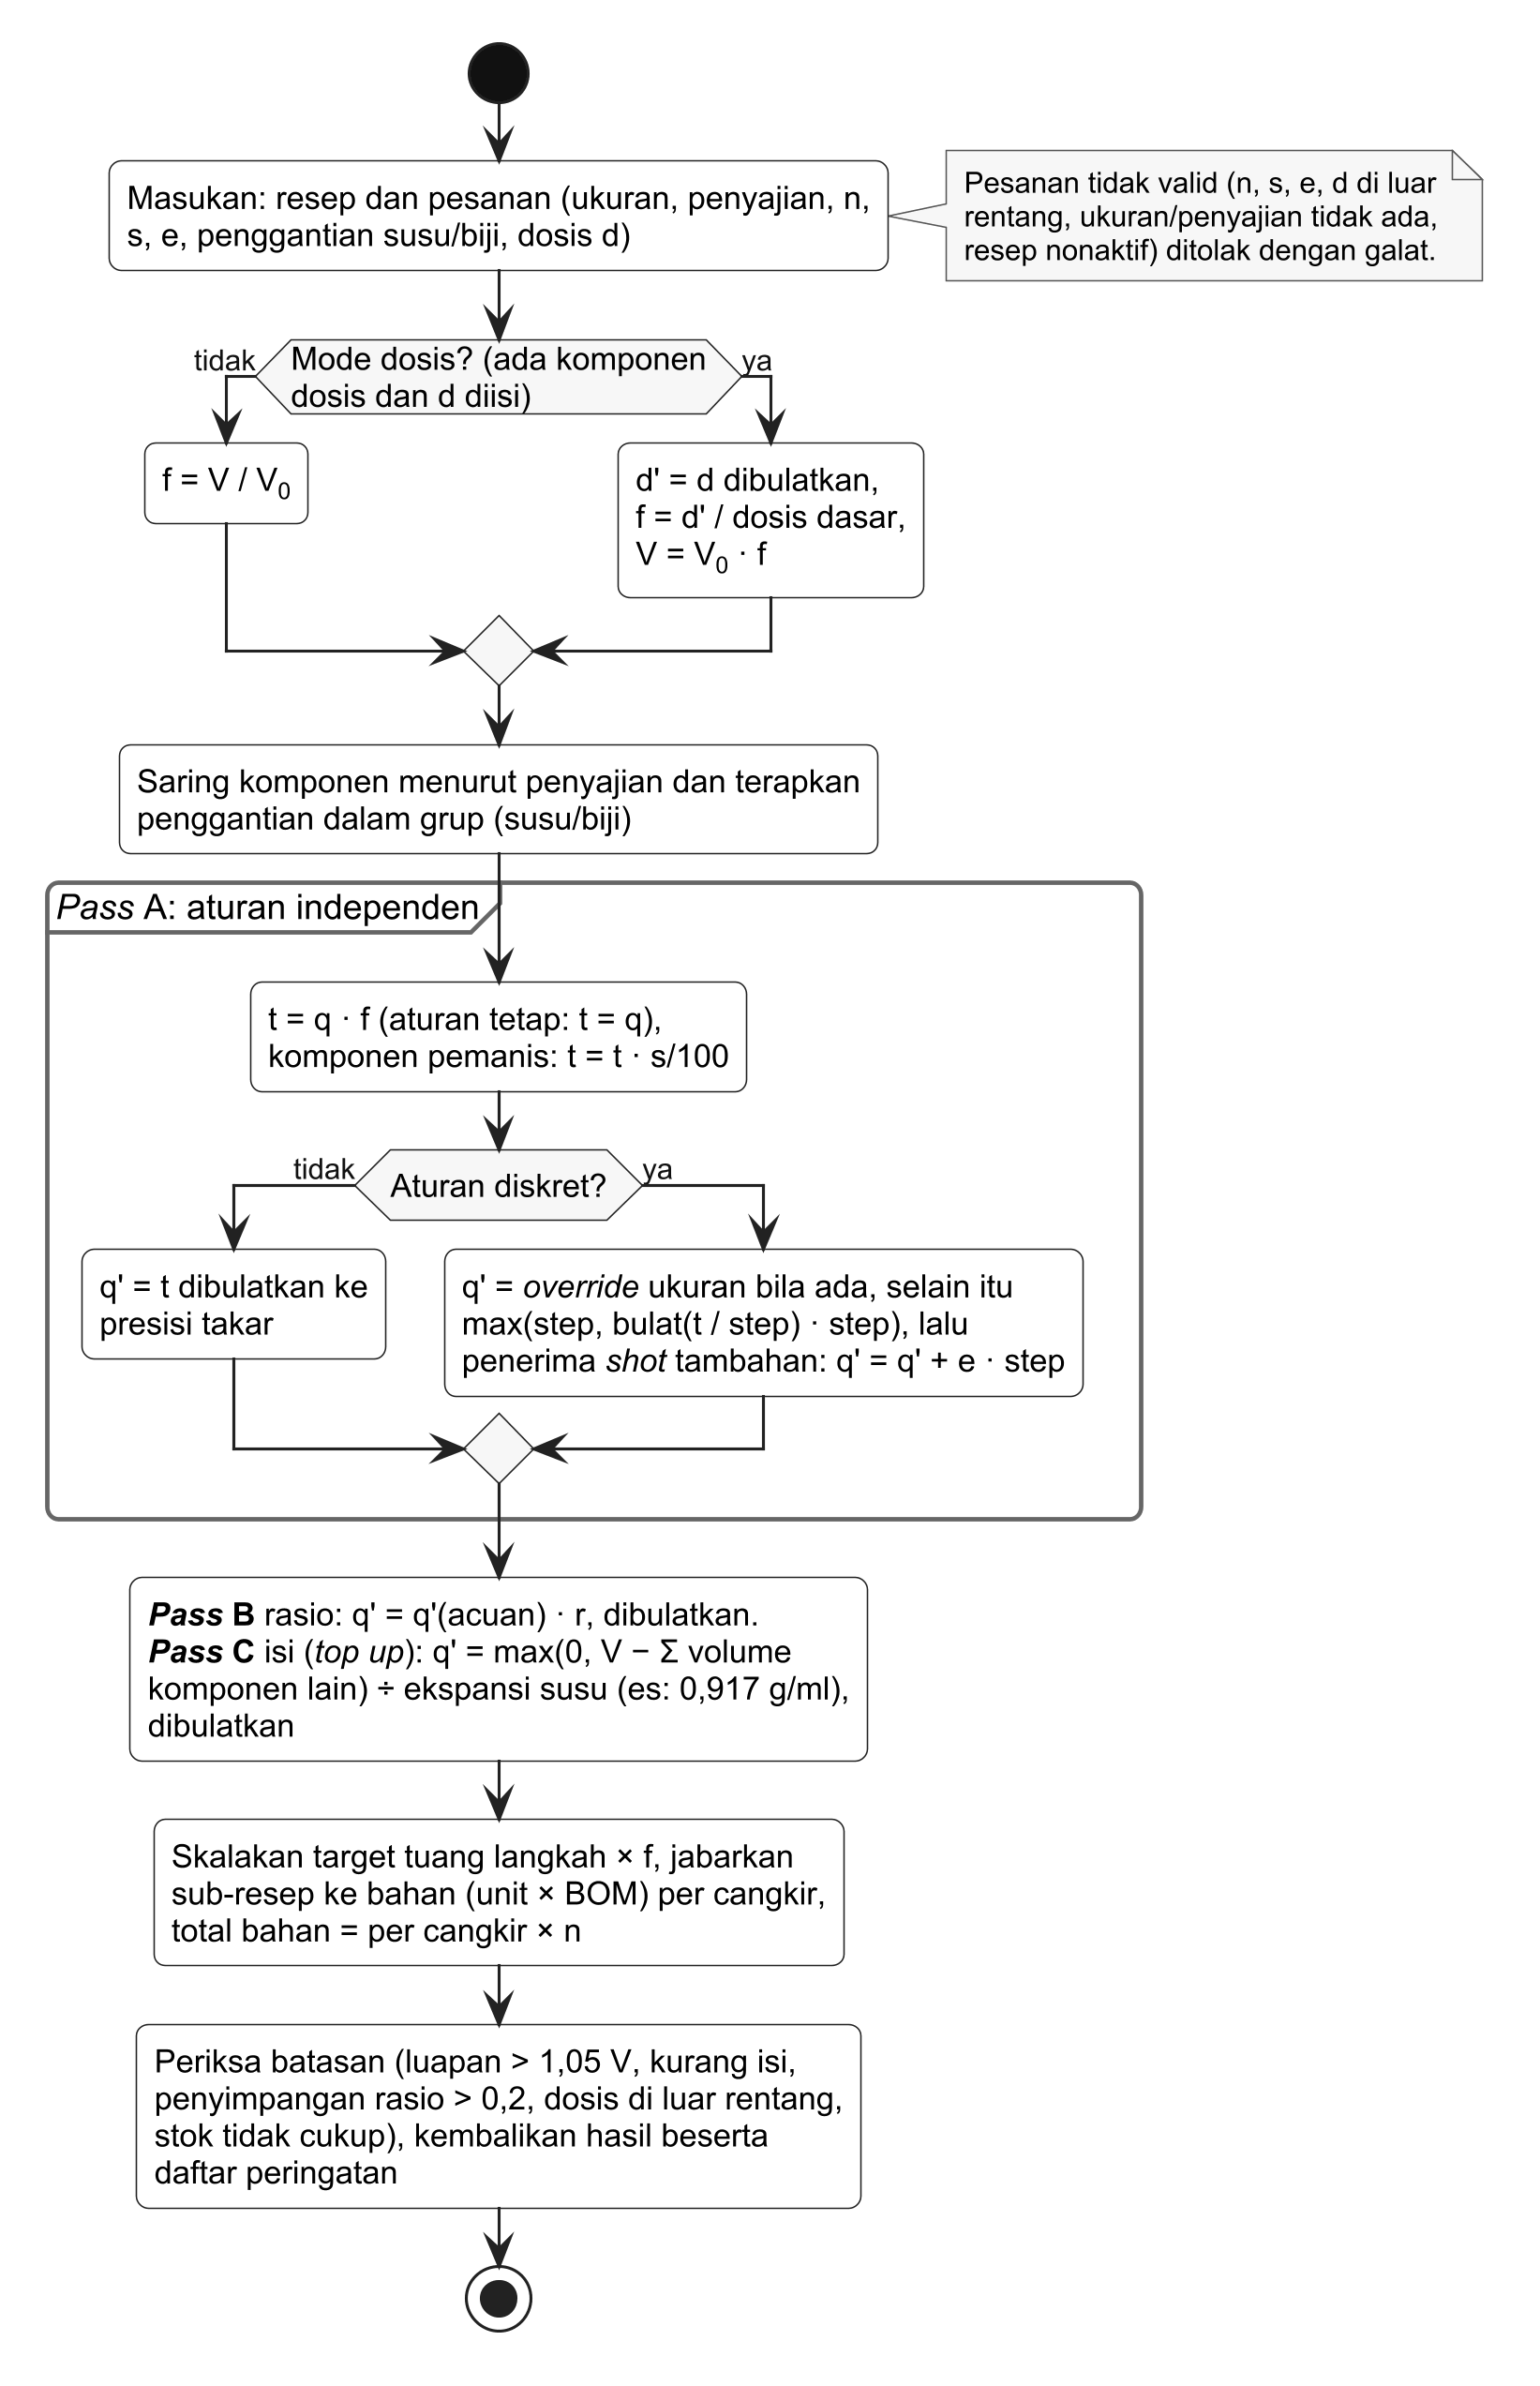
\includegraphics[width=.88\textwidth]{pic/alur_penskalaan.png}
\caption{Alur Aturan Penskalaan dan Pemeriksaan Batasan}
\label{fig:alur-penskalaan}
\end{figure}

\subsection{Pasangan Menu dan Peramalan}

Transaksi IBM dibentuk menjadi keranjang berdasarkan outlet, tanggal, dan nomor struk. Produk dengan ukuran berbeda dinormalisasi menjadi kunci menu yang sama, lalu FP-Growth menambang itemset dan aturan asosiasi. Rekomendasi menerima item yang sedang dipilih, mencocokkan anteseden aturan, mengurutkan konsekuen menurut \textit{confidence} kemudian \textit{lift}, menghapus duplikat, dan mengisi kekurangan tempat dengan item populer yang ditandai sebagai isian. Aplikasi hanya menampilkan aturan dengan \textit{lift} lebih besar dari satu; seluruh aturan tanpa saringan dinilai tersendiri sebagai ablasi. Produk resep yang tidak ada dalam dataset dapat memakai kunci proksi yang dinyatakan di antarmuka.

Peramalan mengubah baris penjualan Maven menjadi deret unit harian per produk dan outlet, dengan tanggal tanpa transaksi diberi nilai nol. Enam metode dibandingkan: \textit{naive}, \textit{seasonal naive} mingguan, rata-rata bergerak tujuh hari, \textit{simple exponential smoothing}, Holt-Winters aditif, dan \textit{histogram gradient boosting} global. Fitur model global hanya memakai lag dan ringkasan penjualan yang telah tersedia di titik asal ramalan. Setiap origin dilatih ulang dengan data sampai origin tersebut, kemudian menghasilkan tujuh hari ke depan. Model aplikasi dipilih menurut WAPE keseluruhan terendah pada data pengembangan.

\subsection{Rekomendasi Pengisian Ulang}

Prakiraan produk diterjemahkan ke kebutuhan bahan melalui BOM resep. Bagi bahan $i$, kebutuhan selama \textit{lead time} $L_i$ adalah penjumlahan kebutuhan harian yang diramalkan, sedangkan simpangan baku galat harian dari periode kalibrasi digunakan untuk stok pengaman. Dengan periode tinjau $R=1$ hari dan koefisien layanan contoh $z=1{,}65$, rancangan memakai
\begin{equation}
SS_i=z\sigma_i\sqrt{L_i},\qquad
ROP_i=\widehat D_i(L_i)+SS_i,\qquad
S_i=\widehat D_i(L_i+R)+SS_i.
\label{eq:restock}
\end{equation}
Di sini $\widehat D_i(h)$ adalah akumulasi kebutuhan ramalan selama $h$ hari, $\sigma_i$ simpangan baku galat harian, $ROP_i$ titik pemesanan ulang, dan $S_i$ tingkat persediaan sasaran. Jumlah yang disarankan adalah selisih positif antara $S_i$ dan posisi stok, dibulatkan ke ukuran kemasan. Angka $z$, \textit{lead time}, dan ukuran kemasan dalam demonstrasi merupakan asumsi, bukan hasil pengukuran pemasok kedai. Gambar~\ref{fig:sequence-restock} memperlihatkan aliran dari ramalan produk menuju kebutuhan bahan dan saran pesan.

\begin{figure}[htbp]
\centering
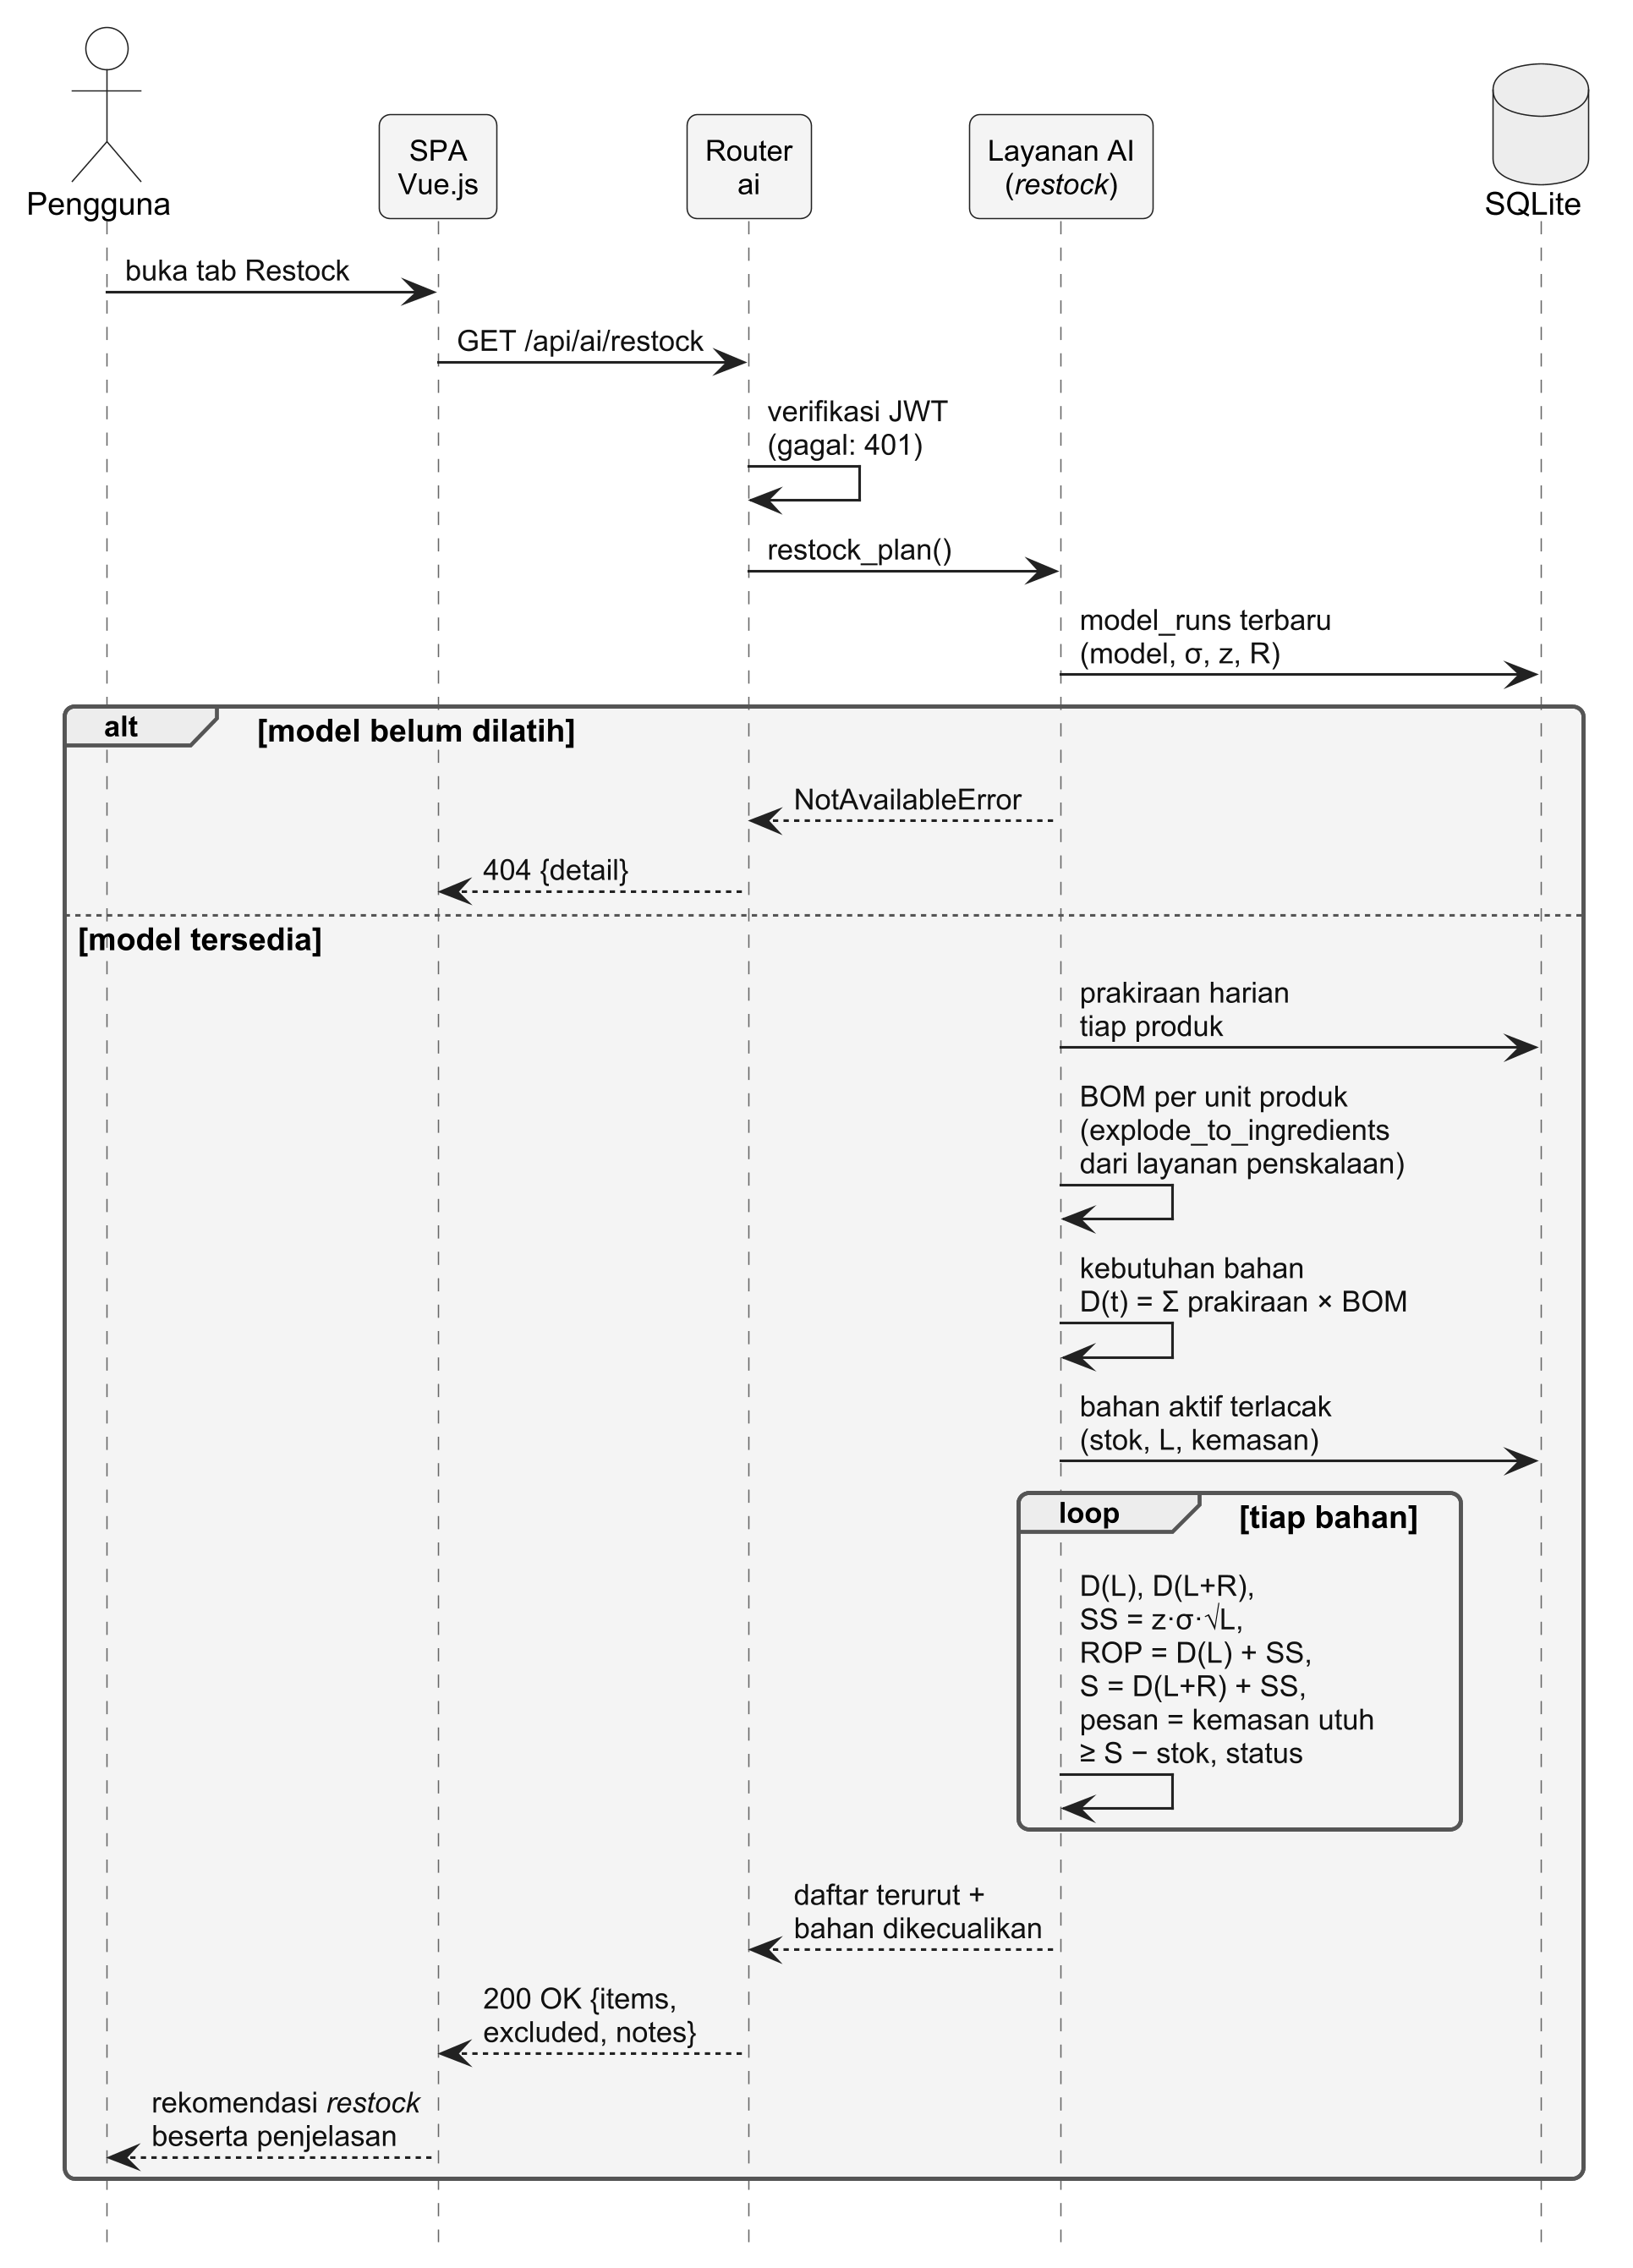
\includegraphics[width=.82\textwidth]{pic/sequence_restock.png}
\caption{Sekuens Peramalan dan Rekomendasi Pengisian Ulang}
\label{fig:sequence-restock}
\end{figure}

\subsection{Sistem Pakar Koreksi Seduh}

Sistem pakar menerima metode, dosis, massa air atau minuman, TDS bila tersedia, waktu, suhu, dan deskriptor rasa. Sistem menghitung rasio dan rendemen ekstraksi (EY) jika masukan cukup, lalu menolak kombinasi fisik yang tidak masuk akal. Basis pengetahuan JSON menyimpan kondisi, kesimpulan, prioritas, saran, dan sumber setiap aturan. Mesin inferensi \textit{forward chaining} memilih aturan cocok dengan prioritas tertinggi, menambahkan fakta baru, dan mengulang sampai tidak ada aturan yang dapat ditembakkan. Jejak aturan disajikan sebagai penjelasan diagnosis. Tabel~\ref{tab:aturan-pakar} meringkas kelompok aturan; ambang lengkap dan sumbernya disimpan dalam \texttt{app/backend/app/ai/kb/brew\_rules.json}.

\begin{table}[htbp]
\centering
\caption{Kelompok Aturan Sistem Pakar Koreksi Seduh}
\label{tab:aturan-pakar}
\begin{tabular}{p{.24\textwidth}p{.63\textwidth}}
\toprule
Kelompok & Tujuan aturan \\
\midrule
Validasi & Menolak input fisik yang tidak wajar atau satuan yang tidak sesuai. \\
Klasifikasi & Menentukan kekuatan dan tingkat ekstraksi dari TDS dan EY bila tersedia. \\
Standar resep & Membandingkan rasio, waktu, dan suhu terhadap resep atau standar literatur yang ditandai sumbernya. \\
Koreksi & Menyarankan perubahan gilingan, rasio, waktu, atau suhu sesuai gejala dan fakta yang tersedia. \\
Penjelasan & Menampilkan aturan yang ditembakkan dan alasan kondisi cocok. \\
\bottomrule
\end{tabular}
\end{table}

\subsection{Perancangan Asisten Barista AI}
\label{subsec:perancangan-asisten}

Asisten tanya-jawab memakai model bahasa yang dijalankan secara lokal melalui Ollama. Korpusnya dibangun dari resep, SOP, aturan sistem pakar, dan glosarium aplikasi; setiap potongan mempunyai pengenal serta tautan ke halaman asal. Pencarian BM25 mengambil potongan paling relevan dan menyediakan konteks yang dapat dikutip. Untuk pertanyaan praktis dengan maksud, entitas katalog, dan parameter yang cukup jelas, router deterministik terlebih dahulu menjalankan alat baca-saja yang memanggil layanan takaran, diagnosis, stok, atau pasangan menu; jawaban ini ditandai sebagai mode alat. Bila parameter untuk alat belum cukup, sistem dapat meminta rincian tanpa mengarang masukan. Pertanyaan lain diberikan kepada model bersama konteks yang ditemukan dan alat yang dapat dipanggil, dengan instruksi untuk menjawab dalam bahasa Indonesia, menyebut sumber, dan menyatakan ketidaktahuan bila fakta tidak tersedia. Pertanyaan di luar cakupan disaring sebelum model dipanggil. Saat model tidak tersedia atau penjaga jawaban menolak keluarannya, pencarian memberi cuplikan sumber dengan penanda mode pencarian yang jelas. Susunan ini adalah pipeline hibrida; hasil alat maupun penolakan dari aturan tidak boleh diatribusikan semata-mata kepada kemampuan Gemma 4.

Empat kondisi evaluasi dipisahkan: pencarian saja, model bahasa tanpa konteks, model dengan \textit{retrieval}, dan model dengan \textit{retrieval} serta alat. Tolok ukur tanya-jawab berbahasa Indonesia disiapkan dengan bantuan AI dari sumber resep, SOP, dan basis aturan; kutipan serta kunci jawaban diperiksa secara otomatis terhadap sumbernya, sedangkan jawaban numerik dihitung oleh layanan aplikasi pada waktu evaluasi. Metriknya mencakup ketepatan pencarian, ketepatan jawaban, pemilihan alat, penolakan pertanyaan di luar cakupan, angka tanpa dasar, latensi, dan jumlah peralihan ke mode pencarian. Tingkat halusinasi angka dihitung sebagai jumlah angka jawaban tanpa dukungan pertanyaan, sumber terambil, atau keluaran alat dibagi seluruh angka yang muncul dalam jawaban. H5 didukung hanya bila, pada model utama Gemma 4 E4B dan butir yang sama, akurasi jawaban kondisi RAG dengan alat lebih tinggi \emph{dan} tingkat halusinasi angkanya lebih rendah daripada kondisi tanpa konteks; Gemma 4 E2B menjadi pembanding tambahan. Butir serta penilaiannya belum mendapat peninjauan manual oleh peneliti maupun barista praktik, sehingga hasilnya bersifat tolok ukur internal dan belum dapat digeneralisasi ke penggunaan kedai.

Tolok ukur internal memuat 60 pertanyaan: 14 fakta resep, 12 prosedur/SOP, 10 perhitungan, delapan diagnosis seduh, enam stok, dan 10 di luar cakupan. Enam kondisi model berasal dari kombinasi tiga konfigurasi (tanpa konteks, RAG, serta RAG dengan alat) dan dua ukuran Gemma 4 (E4B dan E2B); pencarian BM25 tanpa model menjadi kondisi ketujuh. Evaluasi memakai suhu model nol dan \textit{seed} tetap 42, serta menyimpan jawaban mentah agar pemeriksaan skor dapat diulang tanpa memanggil model kembali.

Skor kondisi RAG dengan alat mencakup router deterministik, pemeriksaan luar cakupan, keluaran model, dan peralihan ke pencarian bila diperlukan. Karena itu, perbandingan H5 menilai sistem lengkap pada pertanyaan yang sama, bukan kemampuan model bahasa secara terisolasi. Selain akurasi isi yang menjadi ukuran utama H5, akurasi terverifikasi alat mensyaratkan nama alat dan argumen yang benar pada butir alat. Jumlah jawaban menurut mode alat, model, atau pencarian dilaporkan agar kontribusi masing-masing jalur dapat dibedakan. Akurasi khusus mode model dihitung hanya pada butir yang benar-benar dijawab model dan tidak dapat dibandingkan langsung sebagai kondisi pada keseluruhan 60 butir. Perutean alat disempurnakan setelah kegagalan pada butir tolok ukur awal terlihat; pengujian akhir pada butir yang sama adalah uji regresi internal, bukan estimasi generalisasi independen. Kueri tambahan di luar tolok ukur hanya berfungsi sebagai pemeriksaan cepat dan belum menjadi himpunan uji yang divalidasi manusia.

\section{\texorpdfstring{\textit{Dataset}}{Dataset}}
\label{sec:dataset}

Tabel~\ref{tab:dataset} memisahkan sumber pengembangan dari sumber validasi eksternal. Data mentah disimpan apa adanya di \texttt{dataset/raw}; salinan yang dinormalisasi berada di \texttt{dataset/processed}. Berkas \texttt{DATASHEET.md} pada setiap folder mencatat asal, lisensi, isi, dan keterbatasan. Hash berkas masukan tersimpan dalam hasil eksperimen sehingga perubahan data dapat dideteksi.

\begin{table}[htbp]
\centering
\caption{Sumber Data dan Perannya dalam Penelitian}
\label{tab:dataset}
\begin{tabular}{p{.23\textwidth}p{.22\textwidth}p{.17\textwidth}p{.25\textwidth}}
\toprule
Sumber & Sifat data & Jumlah utama & Penggunaan \\
\midrule
IBM Coffee Shop Sample Data & Sampel fiktif & 49.894 baris & Pengembangan pasangan menu. \\
Maven Coffee Shop Sales & Sampel fiktif & 149.116 baris & Pengembangan peramalan dan \textit{restock}. \\
The Bread Basket & Transaksi nyata; lisensi tidak jelas & 21.293 baris mentah & Validasi pasangan menu (E1). \\
ihelon Coffee Sales & Transaksi nyata; CC0 & 3.636 cangkir & Validasi peramalan dan \textit{restock} (E2--E3). \\
UC Davis/Cotter dan Batali & Eksperimen seduh nyata & 3.186 penilaian; 27 resep & Validasi sistem pakar (E4). \\
Menu Starbucks & Data menu terbitan publik & 7 minuman terpilih & Validasi aturan \textit{shot} per ukuran (E5). \\
\bottomrule
\end{tabular}
\end{table}

Produk publik dipetakan ke resep melalui berkas \texttt{product\_recipe\_map.json}. Tabel~\ref{tab:pemetaan-produk} memberi contoh yang menentukan kebutuhan bahan; pemetaan lengkap beserta asumsi ukuran terdapat pada berkas tersebut dan \texttt{ASSUMPTIONS.md}. Produk kemasan atau roti tanpa resep tidak dipaksakan menjadi minuman dan tidak ikut diuraikan menjadi bahan. Pemetaan ini adalah pendekatan untuk eksperimen, bukan catatan resep asli dari penerbit dataset.

\begin{table}[htbp]
\centering
\caption{Contoh Pemetaan Produk Dataset ke Resep}
\label{tab:pemetaan-produk}
\begin{tabular}{p{.38\textwidth}p{.42\textwidth}}
\toprule
Kelompok produk & Resep aplikasi atau perlakuan \\
\midrule
Latte, Cappuccino, Espresso & Caffè Latte, Cappuccino, Espresso Double. \\
Seduhan kopi tetes & V60 dengan biji yang dipetakan. \\
Cokelat panas, chai, teh & Resep tambahan Hot Chocolate, Chai Latte, Brewed Tea. \\
Sirup tambahan & Komponen bahan tambahan dengan takaran asumsi. \\
Roti dan barang kemasan & Produk akhir; tidak diuraikan menjadi bahan. \\
\bottomrule
\end{tabular}
\end{table}

\section{Rancangan Eksperimen dan Metrik Evaluasi}
\label{sec:rancangan-eksperimen}

Penskalaan diuji pada kombinasi resep jual, ukuran dan sajian yang sah, tingkat manis yang berlaku, tambahan \textit{shot}, jumlah cangkir, serta dosis V60 10--30~g. Tiga metode dijalankan pada pesanan yang sama. Tingkat pelanggaran dihitung untuk \textit{shot} pecahan, luapan lebih dari 5\%, kurang isi, penyimpangan rasio lebih dari 0,2, jumlah di luar batas, ketelitian takar yang tidak praktis, dan ketidaksesuaian jumlah batch. Pemeriksaan yang dijamin oleh bentuk algoritma ditandai sebagai hasil \textit{by construction}; nilai nol pada metrik demikian bukan bukti uji lapangan. Validasi E5 memakai jumlah \textit{shot} yang tersirat dari kafein menu sebagai pembanding eksternal dan membedakan aturan diskret dari tabel pengecualian yang mengambil angka menu itu sendiri.

Pasangan menu dibagi menurut waktu: periode awal untuk latih, bagian akhir latih untuk memilih ambang, dan periode terakhir untuk uji. Pada tiap keranjang uji dengan paling sedikit dua item berbeda, satu item disembunyikan bergantian. HR@1/3/5, Precision@5, MRR@5, cakupan kueri, dan cakupan katalog dibandingkan antara popularitas, peluang ko-okurensi, dan FP-Growth. Selang kepercayaan 95\% didapat dari \textit{bootstrap} keranjang, termasuk selisih berpasangan. Keranjang Maven didefinisikan secara heuristik dari toko, tanggal, dan waktu yang sama karena sumber itu tidak mempunyai nomor struk; hasilnya hanya analisis sekunder. E1 mengulang protokol pada nomor transaksi nyata Bread Basket.

Peramalan dinilai dengan delapan origin mingguan dan horizon tujuh hari. Pada setiap origin, model hanya boleh memakai pengamatan yang terjadi sampai origin tersebut. MAE dan RMSE menunjukkan besaran galat, WAPE mengukur galat absolut terhadap volume permintaan, MASE membandingkan dengan skala \textit{seasonal naive} pada data latih, dan bias menunjukkan arah kesalahan; bias positif berarti ramalan terlalu tinggi. Selain pada produk, ramalan diuraikan melalui BOM menjadi satuan bahan. E2 menguji model yang dipilih pada Maven tanpa memilih ulang model memakai jendela uji ihelon, baik per minuman maupun pada total harian.

Simulasi \textit{restock} memutar ulang 56 hari terakhir permintaan bahan. Kebijakan ramalan tingkat sasaran dibandingkan dengan ROP statis dan tingkat persediaan par; varian pembanding mengendalikan struktur pemesanan dan pilihan model ramalan. Ukuran utama adalah \textit{fill rate}, jumlah hari kehabisan stok, rata-rata stok dalam hari permintaan, dan frekuensi pesanan. Setiap kebijakan menerima stok awal dan asumsi pasokan yang sama. E3 mengulang pada permintaan ihelon yang dipetakan ke tiga bahan demo; keputusan H4 hanya berlaku pada perbandingan kebijakan utama dan ROP statis, bukan pada klaim bahwa model ramalannya terbaik.

Sistem pakar dinilai dari reproduksi EY, kesesuaian arah klasifikasi kekuatan terhadap penilaian konsumen, dan arah koreksi terhadap perubahan parameter pada resep eksperimen. Angka kesukaan konsumen juga dibandingkan di dalam dan di luar kotak \textit{Golden Cup}; kotak tersebut tidak didefinisikan sebagai label kesukaan yang pasti. Pengujian ini membedakan ketepatan perhitungan dari kecocokan preferensi inderawi. Uji asisten lokal mengikuti rancangan pada Subbab~\ref{subsec:perancangan-asisten} dan dilaporkan hanya setelah berkas hasilnya tersedia.

\section{Rancangan Pengujian}
\label{sec:rancangan-pengujian}

Pengujian unit memeriksa aturan penskalaan, buku besar stok, sistem pakar, dan pembantu model AI. Pengujian API memeriksa respons berhasil, nilai batas, masukan tidak sah, serta pembatasan peran. Pengujian \textit{end-to-end} menjalankan alur masuk, resep, kalkulator, produksi, SOP, stok, rekomendasi, dan tampilan ponsel pada hasil \textit{build} yang disajikan server. Basis data uji antarmuka merupakan salinan agar produksi uji tidak mengubah basis data demo. Kasus uji dan hasil aktual ditulis otomatis ke \texttt{app/results/tests}.

Kinerja API diukur setelah pemanasan dengan permintaan berulang pada komputer pengembangan; hasil ini merupakan latensi lingkungan uji, bukan jaminan pada semua perangkat. Audit Lighthouse dilakukan pada halaman masuk publik untuk desktop dan ponsel. Uji penerimaan pengguna dirancang sebagai penyelesaian tugas barista dan kuesioner \textit{System Usability Scale} (SUS) 10 butir. Pelaksanaan bersama pengguna kedai dan nilainya belum tersedia; penelitian ini tidak mengisi skor atau testimoni yang belum dikumpulkan.

\section{Jadwal Penelitian}
\label{sec:jadwal}

Jadwal kegiatan disusun menurut ketergantungan keluaran, seperti pada Tabel~\ref{tab:jadwal}. Tanggal pelaksanaan formal dan sesi uji penerimaan dengan kedai mitra perlu disepakati setelah mitra penelitian dan pembimbing dikonfirmasi. Karena itu, tabel ini menyatakan urutan kerja, bukan tanggal kegiatan yang belum dapat diverifikasi.

\begin{table}[htbp]
\centering
\caption{Urutan Kegiatan Penelitian}
\label{tab:jadwal}
\begin{tabular}{p{.09\textwidth}p{.24\textwidth}p{.50\textwidth}}
\toprule
Urutan & Kegiatan & Keluaran \\
\midrule
1 & Analisis kebutuhan dan sumber & Kebutuhan peran, resep arahan, dan lembar data dataset. \\
2 & Perancangan & Skema data, antarmuka, aturan penskalaan, dan protokol evaluasi. \\
3 & Implementasi bertahap & API, antarmuka, basis pengetahuan, dan skrip model. \\
4 & Pengujian dan evaluasi & Kasus uji, metrik algoritma, dan validasi eksternal. \\
5 & UAT dan penyusunan akhir & Hasil tugas pengguna dan SUS setelah sesi nyata dilaksanakan. \\
\bottomrule
\end{tabular}
\end{table}


% % Bab 4 : Hasil dan Pembahasan
\chapter{\babEmpat}
\label{bab:hasil}
% Semua angka pada bab ini dibaca dari app/results/*.json, app/results/external/*.json,
% app/results/tests/*.xml, app/results/api_latency.json, dan app/results/lighthouse/summary.json.
% Angka dapat berubah bila kode atau data dievaluasi ulang; lihat cap waktu dan hash pada berkas sumber.

\section{Lingkungan Implementasi dan Pengujian}
\label{sec:lingkungan-implementasi}

Takar dijalankan sebagai aplikasi web Vue.js dan API FastAPI dengan basis data SQLite satu berkas. Evaluasi yang tersimpan dijalankan pada Windows 11, Python 3.13.5, prosesor Intel Core i7-12700H, dan memori 31,7~GB. Pengukuran API memakai Uvicorn satu pekerja dan salinan basis data demo berukuran 30,9~MB; pada saat pengukuran terdapat 12 resep, 20 bahan, 80 produk katalog, dan 199.010 baris penjualan yang diimpor. Versi perangkat lunak, hash masukan, waktu, dan parameter eksperimen tersimpan dalam berkas JSON hasil, sehingga metrik pada bab ini adalah hasil lingkungan dan versi tersebut, bukan klaim kinerja universal.

Data pengembangan terdiri atas 49.894 baris IBM untuk pasangan menu dan 149.116 baris Maven untuk peramalan serta simulasi \textit{restock}. Kedua sumber ini adalah data sampel fiktif. Validasi eksternal memakai sumber yang berbeda sifatnya: transaksi Bread Basket dan ihelon, data seduhan konsumen UC Davis dan Batali, serta komposisi kafein menu Starbucks. Pemetaan produk luar ke resep aplikasi adalah asumsi penelitian; berkas pemetaan dan alasan setiap asumsi tersedia bersama kode.

\section{Implementasi Sistem}
\label{sec:implementasi}

Antarmuka menyediakan halaman masuk, beranda, katalog dan detail resep, formulir penyuntingan resep, kalkulator, panduan seduh, SOP dan checklist, inventaris, rekomendasi AI, diagnosis seduh, pengelolaan pengguna, serta data dan model. Kalkulator menampilkan kebutuhan per cangkir, total bahan, stok yang tersedia, peringatan, dan perbandingan dengan hasil linier. Ketika barista mencatat produksi, server menulis log produksi dan satu pergerakan pemakaian untuk setiap bahan hasil uraian BOM. Pengenal permintaan klien dipakai agar pengiriman ulang tidak mengurangi stok dua kali.

Resep arahan pembimbing ditanamkan sebagai basis pengetahuan dengan nilai yang berasal dari dokumen tersebut ditandai sumbernya. Angka yang tidak tersedia di arahan, misalnya ukuran gelas tertentu, stok awal, takaran subresep espreso, \textit{lead time}, dan kemasan pemasok, dinyatakan sebagai asumsi. Hak manajer, kepala barista, dan barista diterapkan pada API dan disajikan sesuai peran dalam navigasi. Tampilan ponsel menggunakan navigasi bawah, sedangkan layar lebih lebar memakai bilah samping. Gambar~\ref{fig:hasil-kalkulator} memperlihatkan contoh halaman kalkulator pada hasil \textit{build} yang diuji.

\begin{figure}[htbp]
\centering
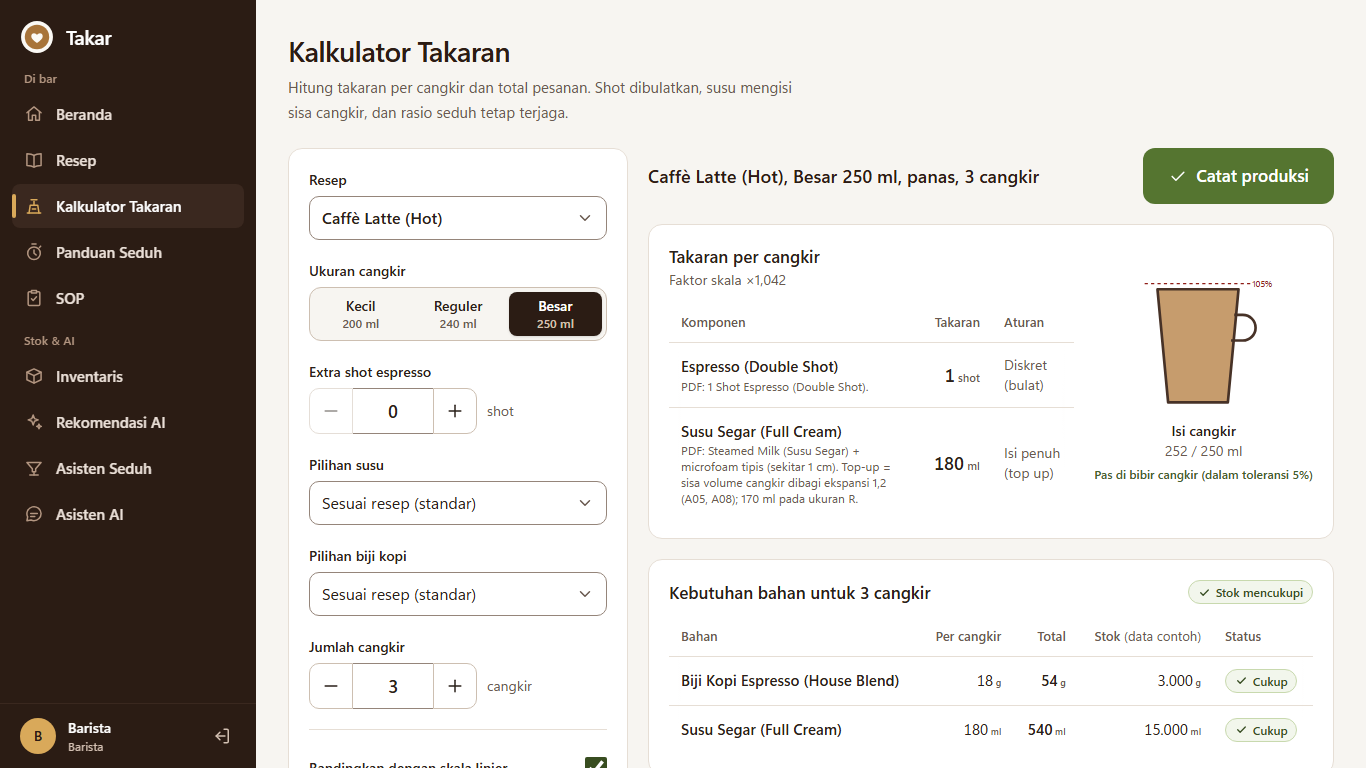
\includegraphics[width=.78\textwidth]{pic/results/screenshots/desktop/07-kalkulator-latte-besar-3-cangkir.png}
\caption{Tampilan Kalkulator Takaran Caffè Latte pada Pengujian Antarmuka}
\label{fig:hasil-kalkulator}
\end{figure}

Panduan Seduh dan Timer Shot menampilkan ilustrasi SVG yang bergerak mengikuti tahap resep aktif, misalnya aliran air pada V60, ekstraksi espreso, atau pengukusan susu. Judul langkah, waktu, target takaran, dan parameter tetap diambil dari data resep; animasi hanya membantu mengenali tindakan dan dapat dijeda, termasuk ketika perangkat meminta pengurangan gerak. Dari rekomendasi pasangan menu, tautan ``Pelajari resep'' membuka panduan bila produk saran mempunyai padanan resep aktif. Alur ini menghubungkan saran menu dengan prosedur yang dapat dipraktikkan, tetapi manfaatnya bagi pembelajaran barista masih memerlukan UAT.

\section{Hasil Pengujian Fungsional}
\label{sec:hasil-fungsional}

% sumber: results/tests/backend.xml, results/tests/e2e.xml, results/tests/blackbox_cases.csv
% sumber: results/tests/backend.xml dan results/tests/blackbox_cases.csv.
Berkas pengujian akhir mencatat 706 kasus \textit{pytest} backend dan 29 kasus \textit{end-to-end} Playwright, semuanya lulus tanpa kegagalan. Kasus antarmuka mencakup masuk dengan tiga peran, penolakan kata sandi keliru, hak akses barista, daftar dan detail resep, variasi kalkulator, pencatatan produksi, mutasi stok, checklist SOP, timer, rekomendasi AI, asisten lokal, animasi seduh, tautan dari saran pasangan ke panduan, serta tampilan ponsel. Berkas \texttt{blackbox\_cases.csv} menyimpan langkah, hasil yang diharapkan, hasil yang benar-benar terbaca pada layar, dan status tiap kasus. Jumlah kasus ini menyatakan cakupan suite otomatis saat berkas dihasilkan; ia tidak menggantikan uji penerimaan oleh barista kedai.

Pengujian layanan juga memeriksa permintaan tanpa token dan peran yang tidak berhak, validasi pesanan, serta transaksi stok. Skenario perhitungan V60 15~g menghasilkan air 225~ml dan target tuang 45, 130, serta 225~ml; pada dosis 20~g kebutuhan air menjadi 300~ml dan target kumulatif 60, 173,3, serta 300~ml. Hasil ini merupakan pemeriksaan terhadap aturan resep yang telah ditetapkan, bukan pengukuran rasa seduhan di lapangan.

\section{Hasil Evaluasi Penskalaan Resep}
\label{sec:hasil-penskalaan}

% sumber: results/scaling_eval.json (summary.methods, headline, parameters)
Grid evaluasi menghasilkan 525 pesanan efektif pada 12 resep jual. Grid itu meliputi tambahan sampai tiga \textit{shot}, sesuai batas masukan API; subset spesifikasi awal sampai dua \textit{shot} memuat 435 pesanan. Tabel~\ref{tab:hasil-penskalaan} membandingkan tiga metode pada 525 pesanan yang sama. Penskalaan berbasis batasan tidak menghasilkan \textit{shot} pecahan, luapan lebih dari 5\%, atau penyimpangan rasio lebih dari 0,2. Penskalaan linier mentah menghasilkan 240 pesanan dengan \textit{shot} pecahan dan 267 luapan; versi linier yang dibulatkan menghapus \textit{shot} pecahan, tetapi menghasilkan 282 luapan. Dengan kriteria H1 yang ditetapkan pada Bab~\ref{bab:pendahuluan}, H1 didukung pada grid ini.

\begin{table}[htbp]
\centering
\caption{Pelanggaran Penskalaan pada 525 Pesanan Uji}
\label{tab:hasil-penskalaan}
\small
\begin{tabular}{lrrr}
\toprule
Pemeriksaan & Berbasis batasan & Linier dibulatkan & Linier mentah \\
\midrule
\textit{Shot} pecahan & 0 & 0 & 240 \\
Luapan cangkir & 0 & 282 & 267 \\
Penyimpangan rasio & 0 & 0 & 0 \\
Ketelitian tidak praktis & 0 & 0 & 300 \\
Jumlah batch tidak konsisten & 0 & 0 & 183 \\
Peringatan kurang isi & 144 & 0 & 0 \\
\bottomrule
\end{tabular}
\end{table}

Nilai nol untuk \textit{shot} pecahan dan ketidaksesuaian jumlah batch pada metode berbasis batasan dijamin oleh aturan diskret dan perkalian takaran per cangkir; karena itu hasil tersebut diberi penanda \textit{by construction}. Selain itu, 144 pesanan berbasis batasan menerima peringatan kurang isi karena jumlah komponen pengisi berada di bawah batas minimum resep. Peringatan ini tidak masuk tiga kriteria H1, tetapi menunjukkan bahwa mencegah luapan saja belum menjamin semua minuman mencapai komposisi yang diinginkan. Pengujian sensorik dan keputusan barista dibutuhkan untuk menilai apakah pesanan seperti itu sebaiknya ditolak atau resepnya disesuaikan.

Gambar~\ref{fig:hasil-skala} memperlihatkan persentase pelanggaran yang dapat membedakan ketiga metode. Penyimpangan rasio bernilai nol pada semua metode di grid tersebut, sehingga tidak ditampilkan dalam grafik.
\begin{figure}[htbp]
\centering
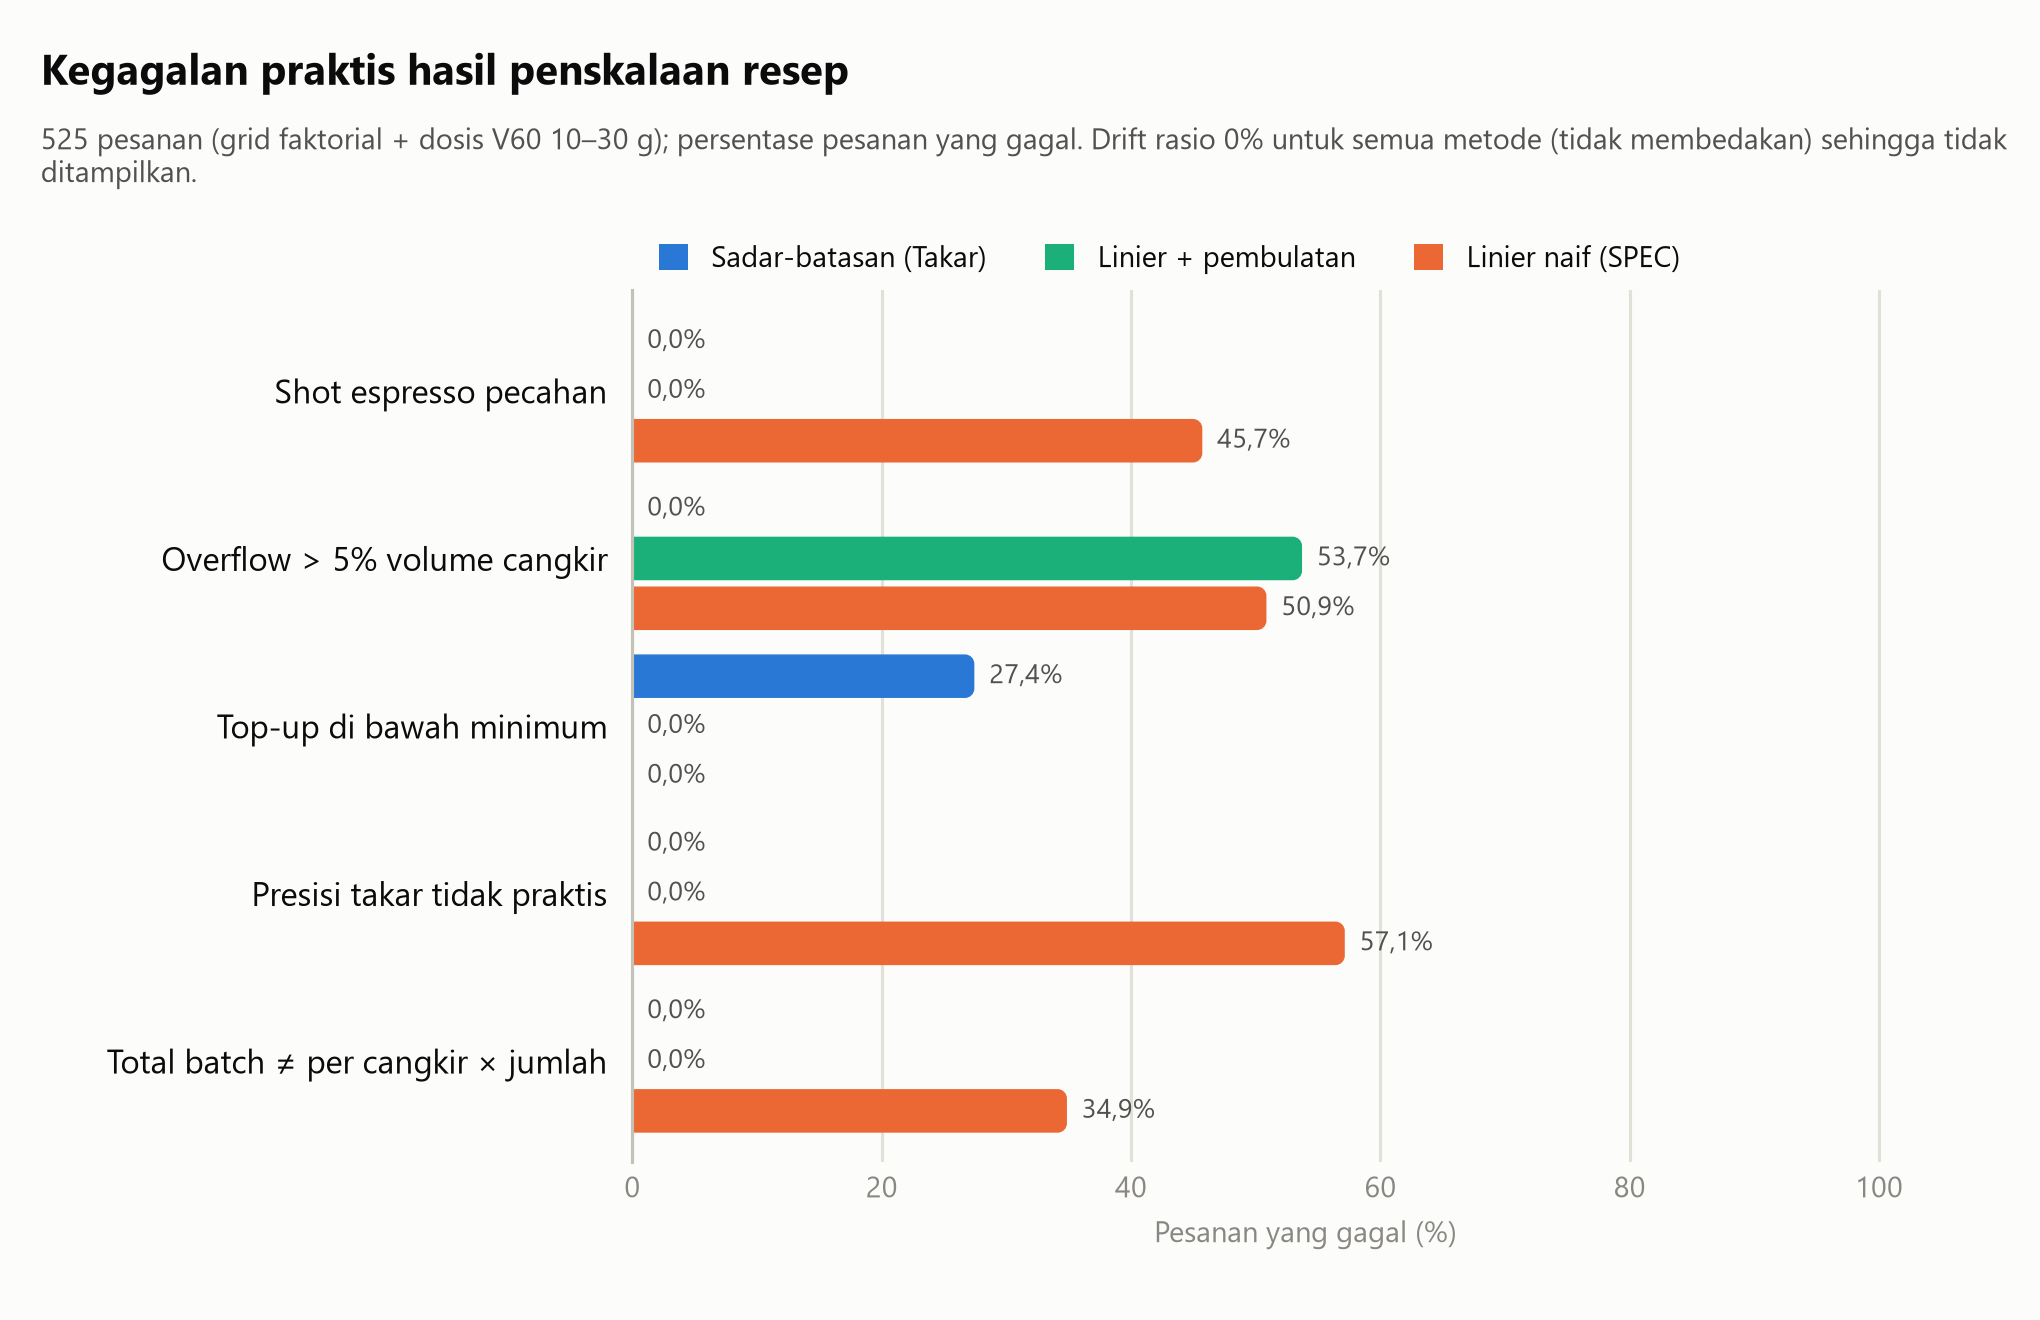
\includegraphics[width=.82\textwidth]{pic/results/figures/scaling_eval.png}
\caption{Kegagalan Praktis pada Grid Penskalaan Resep}
\label{fig:hasil-skala}
\end{figure}

% sumber: results/external/E5_scaling_starbucks.json (headline)
Validasi eksternal E5 memakai tujuh minuman berbasis espreso pada empat ukuran; kombinasi tiga ukuran bukan dasar per minuman menghasilkan 84 prediksi yang dikumpulkan lintas pilihan ukuran dasar. Proporsi hasil linier mentah yang berupa \textit{shot} pecahan adalah 84,5\%, sedangkan aturan diskret menghasilkan 0\% karena sifat konstruksinya. Tingkat kecocokan tepat terhadap jumlah \textit{shot} menu adalah 14,3\% untuk hasil linier mentah dan 58,3\% untuk aturan diskret dengan pembulatan setengah ke atas. Pengecualian ukuran mencapai 100\% karena tabel itu diisi langsung dari jumlah \textit{shot} menu; angka tersebut membuktikan kemampuan representasi, bukan akurasi prediksi. Hasil ini mendukung kebutuhan aturan diskret dan data pengecualian ukuran, tetapi satu menu jaringan di Amerika Serikat tidak mewakili semua kedai kopi.

\section{Hasil Evaluasi Rekomendasi Pasangan Menu}
\label{sec:hasil-pasangan}

% sumber: results/pairing_eval.json; results/external/E1_pairing_breadbasket.json
Pada data sampel fiktif IBM, periode uji 22--29 April 2019 menghasilkan 2.067 keranjang multi-item dan 4.260 kueri \textit{leave-one-out}. FP-Growth yang dipakai aplikasi, yaitu aturan dengan \textit{lift} lebih dari satu, mencapai HR@5 sebesar 0,4941 dan MRR@5 sebesar 0,2902. Popularitas mencapai HR@5 0,1324, sedangkan ko-okurensi mencapai 0,5134. Selisih HR@5 FP-Growth terhadap popularitas 0,3617 dengan selang kepercayaan (IK) \textit{bootstrap} 95\% [0,3402; 0,3839]. Dengan demikian, H2 didukung pada data pengembangan IBM, tetapi ko-okurensi sederhana justru lebih baik pada HR@5.

Pada 1.165 keranjang multi-item nyata Bread Basket, diperoleh 3.167 kueri uji. Tabel~\ref{tab:hasil-pasangan} menunjukkan bahwa HR@5 FP-Growth 0,5718 hanya sedikit di atas popularitas 0,5658. Selisih berpasangan 0,0060 mempunyai IK 95\% [-0,0028; 0,0147], sehingga H2 tidak didukung pada data nyata ini. Ko-okurensi mencapai HR@5 0,6021 dan MRR@5 0,4015, keduanya lebih tinggi daripada FP-Growth yang dipakai aplikasi. Nilai MRR@5 FP-Growth 0,3768 bahkan lebih rendah dari popularitas 0,3871; selisihnya -0,0103 dengan IK 95\% [-0,0199; -0,0005].

\begin{table}[htbp]
\centering
\caption{Kinerja Pasangan Menu pada Data Uji Bread Basket}
\label{tab:hasil-pasangan}
\begin{tabular}{lrrr}
\toprule
Metode & HR@1 & HR@5 & MRR@5 \\
\midrule
Popularitas & 0,2807 & 0,5658 & 0,3871 \\
Ko-okurensi & 0,2851 & 0,6021 & 0,4015 \\
FP-Growth (\textit{lift} $>1$) & 0,2674 & 0,5718 & 0,3768 \\
FP-Growth semua aturan (ablasi) & 0,2839 & 0,5851 & 0,3962 \\
\bottomrule
\end{tabular}
\end{table}

Ablasi tanpa saringan \textit{lift} meningkatkan HR@5 Bread Basket menjadi 0,5851, tetapi bukan metode yang disajikan aplikasi dan tidak dipakai untuk keputusan H2. Salah satu penyebab yang ditemukan adalah saringan \textit{lift} membuang 36 dari 83 aturan menuju Coffee pada periode latih, karena Coffee sendiri sangat populer. Dataset Bread Basket berasal dari satu toko roti-kafe Edinburgh dan lisensi unggahan paling awal tidak jelas; karena itu perbedaan ini menjadi peringatan tentang transfer model, bukan dasar untuk menyatakan seluruh aturan asosiasi tidak berguna.

Perbedaan antarmetode pada data nyata dan IK selisih berpasangan diringkas pada Gambar~\ref{fig:hasil-pasangan-eksternal}. Selang HR@5 FP-Growth dikurangi popularitas memotong nol, sedangkan selang HR@1 dan MRR@5 berada di bawah nol.
\begin{figure}[htbp]
\centering
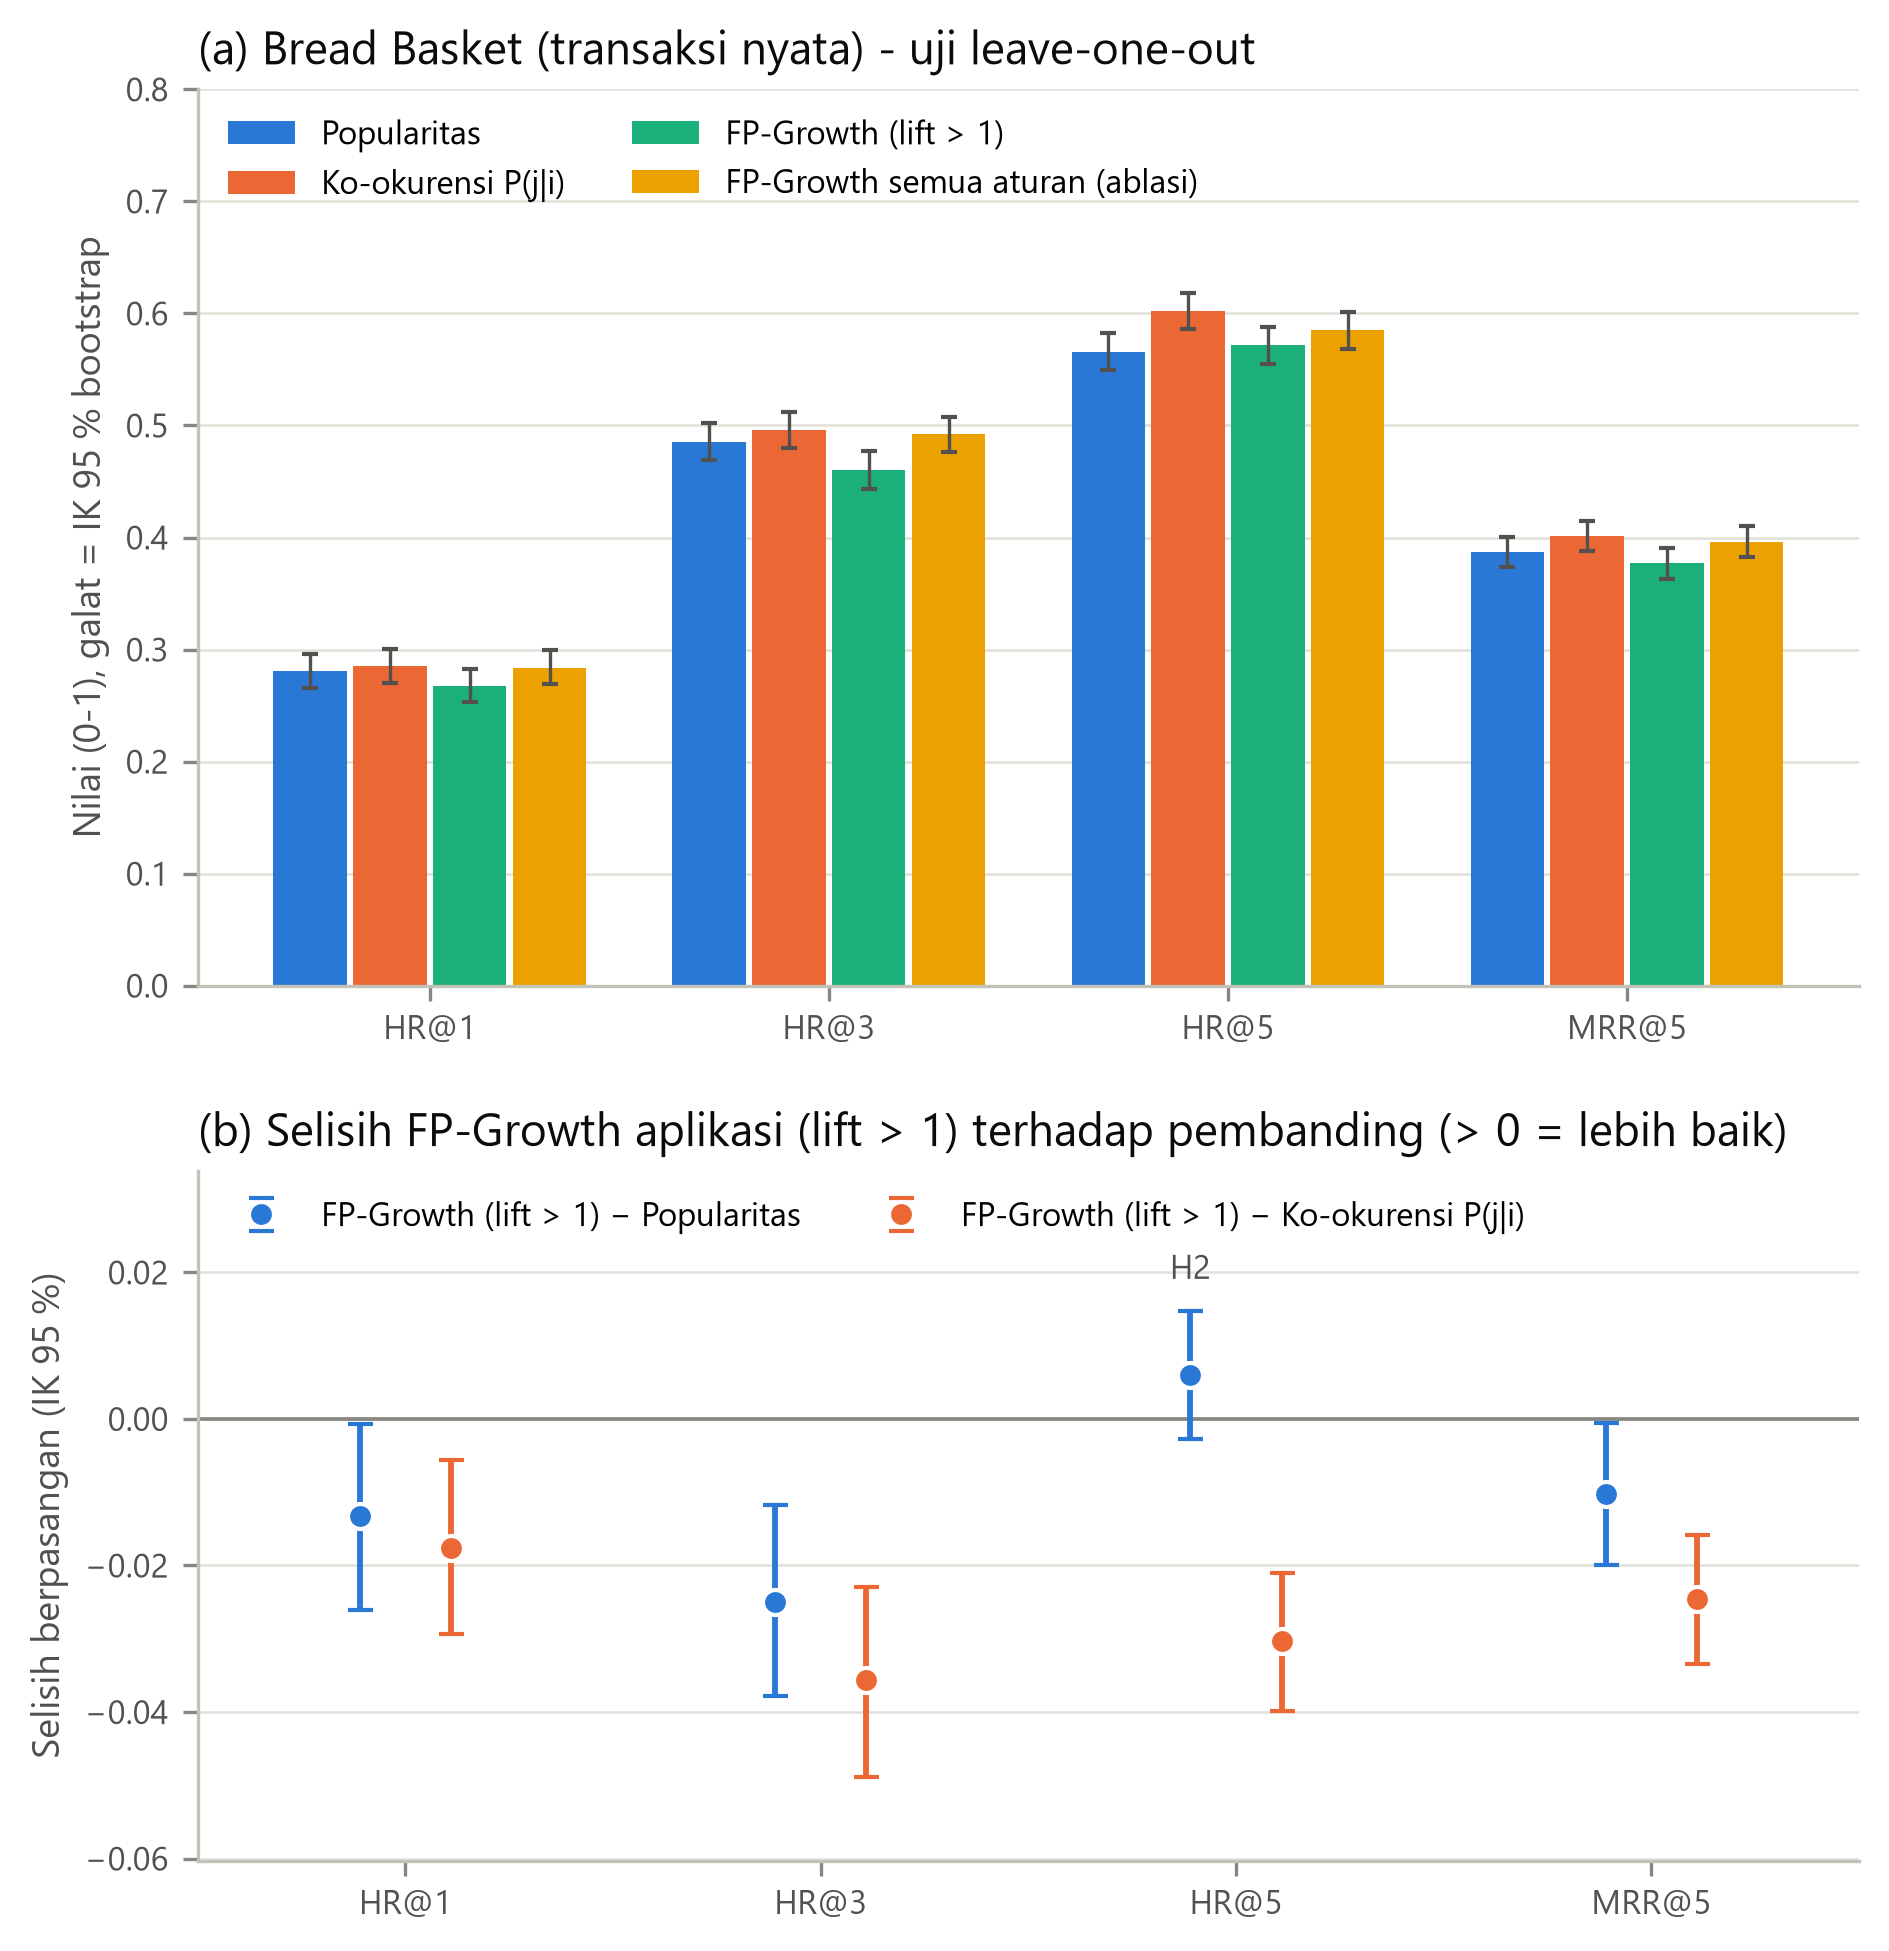
\includegraphics[width=.76\textwidth]{pic/results/figures/external_E1_pairing.png}
\caption{Kinerja Pasangan Menu dan Selisih Berpasangan pada Transaksi Bread Basket}
\label{fig:hasil-pasangan-eksternal}
\end{figure}

\section{Hasil Evaluasi Peramalan Permintaan}
\label{sec:hasil-peramalan}

% sumber: results/forecast_eval.json (data, protocol, overall)
Maven menyediakan 149.116 baris penjualan selama 181 hari, yang dibentuk menjadi 240 deret produk--outlet. Delapan origin mingguan dengan horizon tujuh hari menghasilkan 13.440 titik prediksi per metode. Tabel~\ref{tab:hasil-peramalan} menunjukkan bahwa \textit{gradient boosting} global memperoleh WAPE terendah, 0,3964, dibandingkan \textit{seasonal naive} 0,5381; model itu dipilih untuk aplikasi sebelum data validasi ihelon dinilai. Peramalan produk yang mempunyai pemetaan BOM juga diuraikan menjadi kebutuhan bahan, tetapi ketepatan pada bahan bergantung pada ketepatan pemetaan produk ke resep.

\begin{table}[htbp]
\centering
\caption{Perbandingan WAPE Peramalan pada Data Pengembangan Maven}
\label{tab:hasil-peramalan}
\begin{tabular}{lr}
\toprule
Model & WAPE \\
\midrule
\textit{Gradient boosting} global & 0,3964 \\
\textit{Simple exponential smoothing} & 0,4073 \\
Holt-Winters & 0,4161 \\
Rata-rata bergerak tujuh hari & 0,4266 \\
\textit{Seasonal naive} & 0,5381 \\
\textit{Naive} & 0,5389 \\
\bottomrule
\end{tabular}
\end{table}

% sumber: results/external/E2_forecast_ihelon.json (h3)
Validasi E2 memakai 3.636 cangkir nyata dari satu mesin penjual kopi, delapan minuman, dan delapan origin uji mingguan. Model terpilih mempunyai WAPE per minuman 0,6582 versus \textit{seasonal naive} 0,7125. Selisih -0,0542 ber-IK 95\% [-0,1145; 0,0159], sehingga penurunan estimasi titik belum meyakinkan. Pada total harian yang diramal langsung, WAPE model terpilih 0,3862 justru lebih tinggi daripada \textit{seasonal naive} 0,2646; selisih 0,1216 ber-IK [0,0527; 0,1897]. Maka H3 tidak didukung pada validasi nyata, meskipun model yang sama unggul pada data pengembangan fiktif. Hasil eksploratif model Holt-Winters pada seri per minuman tidak dipakai mengganti keputusan H3 karena model itu dipilih sesudah jendela uji dilihat.

Gambar~\ref{fig:hasil-forecast-eksternal} menampilkan WAPE setiap model pada seri per minuman ihelon. Grafik ini membantu membedakan peringkat eksploratif dari pengujian H3 yang memakai model terpilih sebelumnya.
\begin{figure}[htbp]
\centering
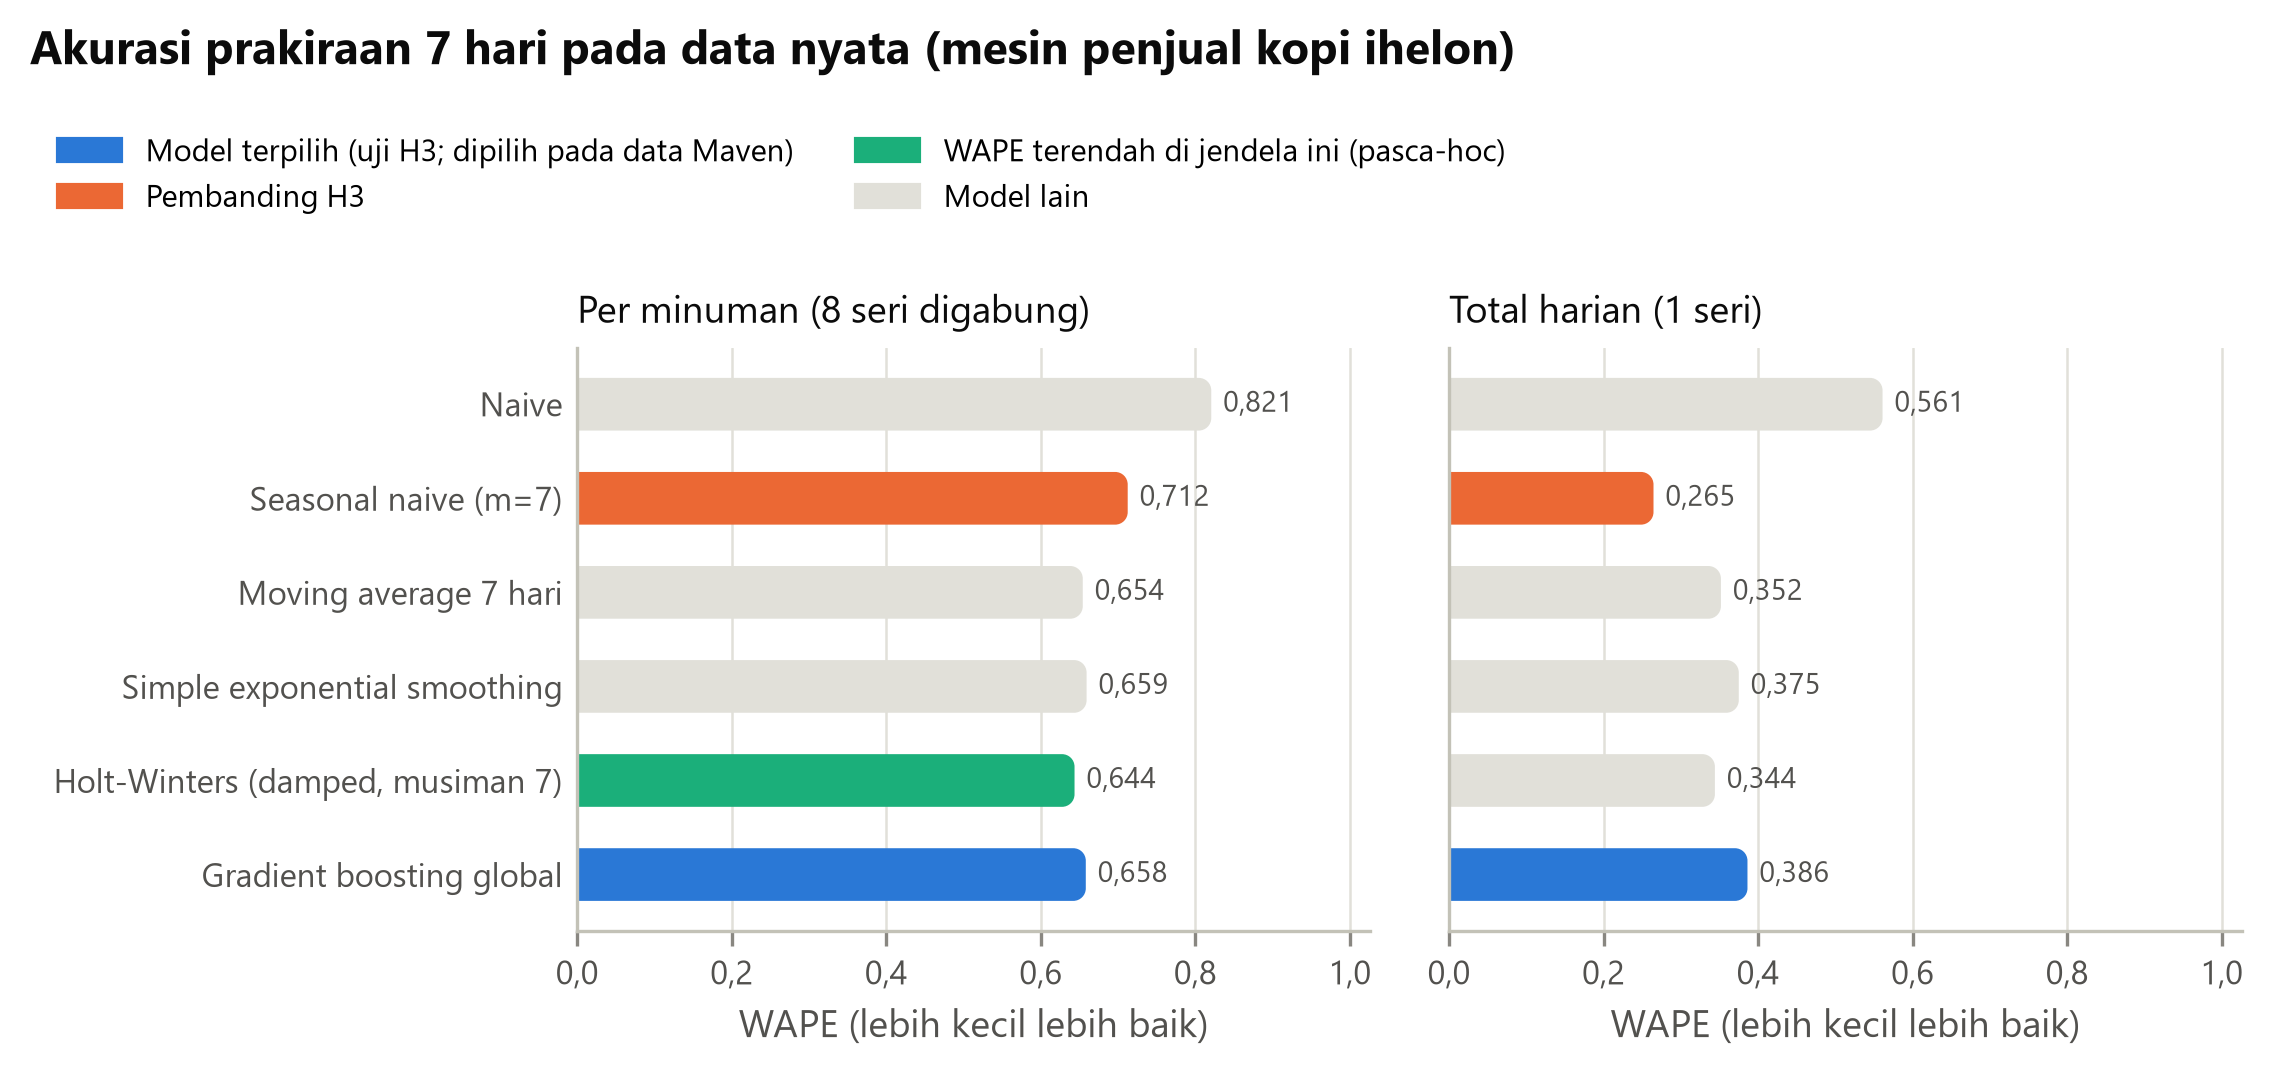
\includegraphics[width=.82\textwidth]{pic/results/figures/external_E2_wape_by_model.png}
\caption{WAPE Peramalan per Minuman pada Data Nyata ihelon}
\label{fig:hasil-forecast-eksternal}
\end{figure}

\section{Hasil Simulasi Rekomendasi \texorpdfstring{\textit{Restock}}{Restock}}
\label{sec:hasil-restock}

% sumber: results/restock_eval.json (summary, data)
Pada replay 56 hari data sampel fiktif Maven untuk 12 bahan, kebijakan tingkat sasaran berbasis prakiraan mencapai \textit{fill rate} rata-rata 0,9748 dan 60 hari kehabisan stok jika dijumlahkan lintas bahan. ROP statis mencapai 0,8173 dan 212 hari, sedangkan tingkat par mencapai 0,7138 dan 210 hari. Rata-rata stok yang dipegang kebijakan prakiraan 3,70 hari permintaan, lebih tinggi daripada ROP statis 2,55 hari. Dengan demikian, kenaikan layanan pada eksperimen ini mempunyai konsekuensi stok tertahan yang perlu dinilai bersama risiko bahan basi dan biaya kedai nyata.

% sumber: results/external/E3_restock_ihelon.json (summary, h4, ablation)
Validasi E3 mengubah transaksi ihelon menjadi permintaan tiga bahan demo. Pada replay 56 hari, kebijakan prakiraan mencapai \textit{fill rate} rata-rata 0,9605 dan 17 hari kehabisan stok, sedangkan ROP statis 0,7900 dan 47 hari. H4 didukung untuk perbandingan yang ditetapkan, dengan selisih \textit{fill rate} 0,1706. Akan tetapi, tingkat sasaran statis dengan struktur pemesanan yang sama sudah mencapai 0,8633; selisih 0,0972 terhadap kebijakan prakiraan memisahkan manfaat tingkat yang berubah dari manfaat struktur. Ketika struktur sama dan hanya model prakiraan diganti, rata-rata bergerak tujuh hari mencapai 0,9871 dan \textit{seasonal naive} 0,9671, keduanya di atas model terpilih 0,9605. H4 karenanya mendukung kebijakan dinamis pada skenario ini, bukan superioritas model \textit{machine learning}. Seluruh hasil bergantung pada \textit{lead time}, stok awal, dan ukuran kemasan yang merupakan data contoh.

Gambar~\ref{fig:hasil-restock-eksternal} memperlihatkan \textit{fill rate} per bahan dan per kebijakan. Perbedaan antarbahan menegaskan bahwa rata-rata tiga bahan tidak boleh dibaca sebagai jaminan tingkat layanan setiap bahan.
\begin{figure}[htbp]
\centering
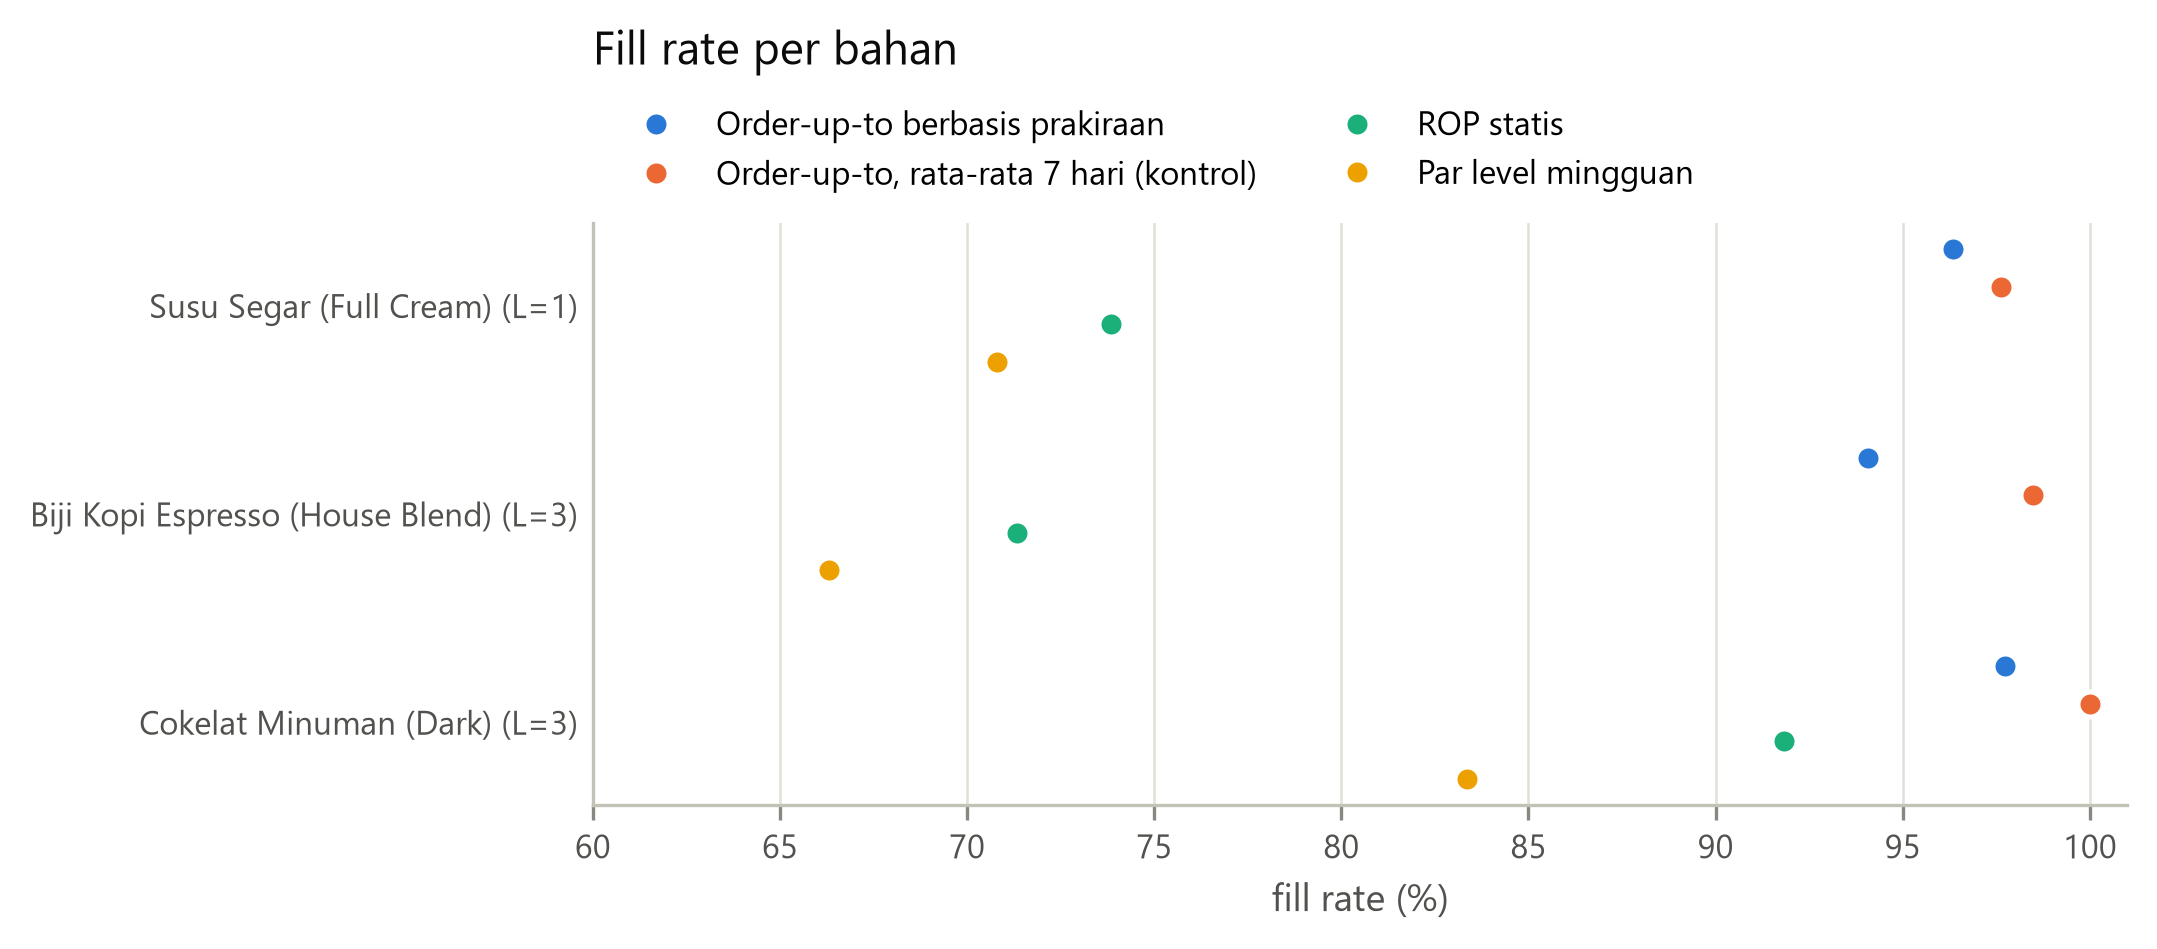
\includegraphics[width=.82\textwidth]{pic/results/figures/external_E3_fill_rate.png}
\caption{Tingkat Pemenuhan Permintaan Bahan pada Replay ihelon}
\label{fig:hasil-restock-eksternal}
\end{figure}

\section{Hasil Pengujian Sistem Pakar}
\label{sec:hasil-sistem-pakar}

% sumber: results/external/E4_expert_validation.json
Validasi E4 memakai 3.186 penilaian konsumen atas 162 seduhan; satu seduhan dengan EY di atas batas fisik ditolak, sehingga 3.164 penilaian atas 161 seduhan dapat dianalisis. Pada seduhan yang mempunyai massa minuman terukur, rumus EY mesin sama dengan nilai dataset sampai galat maksimum sekitar $5\times10^{-9}$ poin persentase. Ini memeriksa ketepatan perhitungan, bukan ketepatan diagnosis rasa. Basis aturan yang dipakai berisi 64 aturan.

Di antara penilaian \textit{just-about-right} yang bukan kategori pas pada seduhan yang ditandai lemah atau kuat oleh sistem, 820 dari 1.067 penilaian sesuai arah diagnosis, yaitu 76,9\% (IK 95\% [73,8\%; 80,0\%]). Kesepakatan berbeda menurut kelas: 89,5\% untuk lemah dan 60,7\% untuk kuat. Rerata kesukaan seduhan di dalam kotak \textit{Golden Cup} 5,812, sedangkan di luar 5,854; selisih -0,042 ber-IK 95\% [-0,233; 0,145]. Karena selang ini memuat nol dan preferensi konsumen bervariasi, sistem tidak menganggap kotak itu sebagai jaminan kesukaan.

Pada 27 resep eksperimen Batali, perbandingan arah koreksi yang dapat dinilai terhadap kotak acuan menunjukkan 26 dari 34 pasangan searah untuk tuas ekstraksi dan 12 dari 12 untuk tuas kekuatan. Sejumlah pasangan tidak menghasilkan saran tuas karena sudah berada pada pita target atau dibatasi fakta lain. Penelitian ini hanya membandingkan arah perubahan parameter yang diamati; ia tidak membuktikan bahwa semua saran sistem akan memperbaiki rasa bila diterapkan oleh barista pada bahan dan peralatan lain.

Sebaran TDS dan EY seduhan UC Davis terhadap kotak teknis ditunjukkan pada Gambar~\ref{fig:hasil-kendali-seduh}. Titik di dalam kotak adalah klasifikasi teknis, bukan label kesukaan peserta.
\begin{figure}[htbp]
\centering
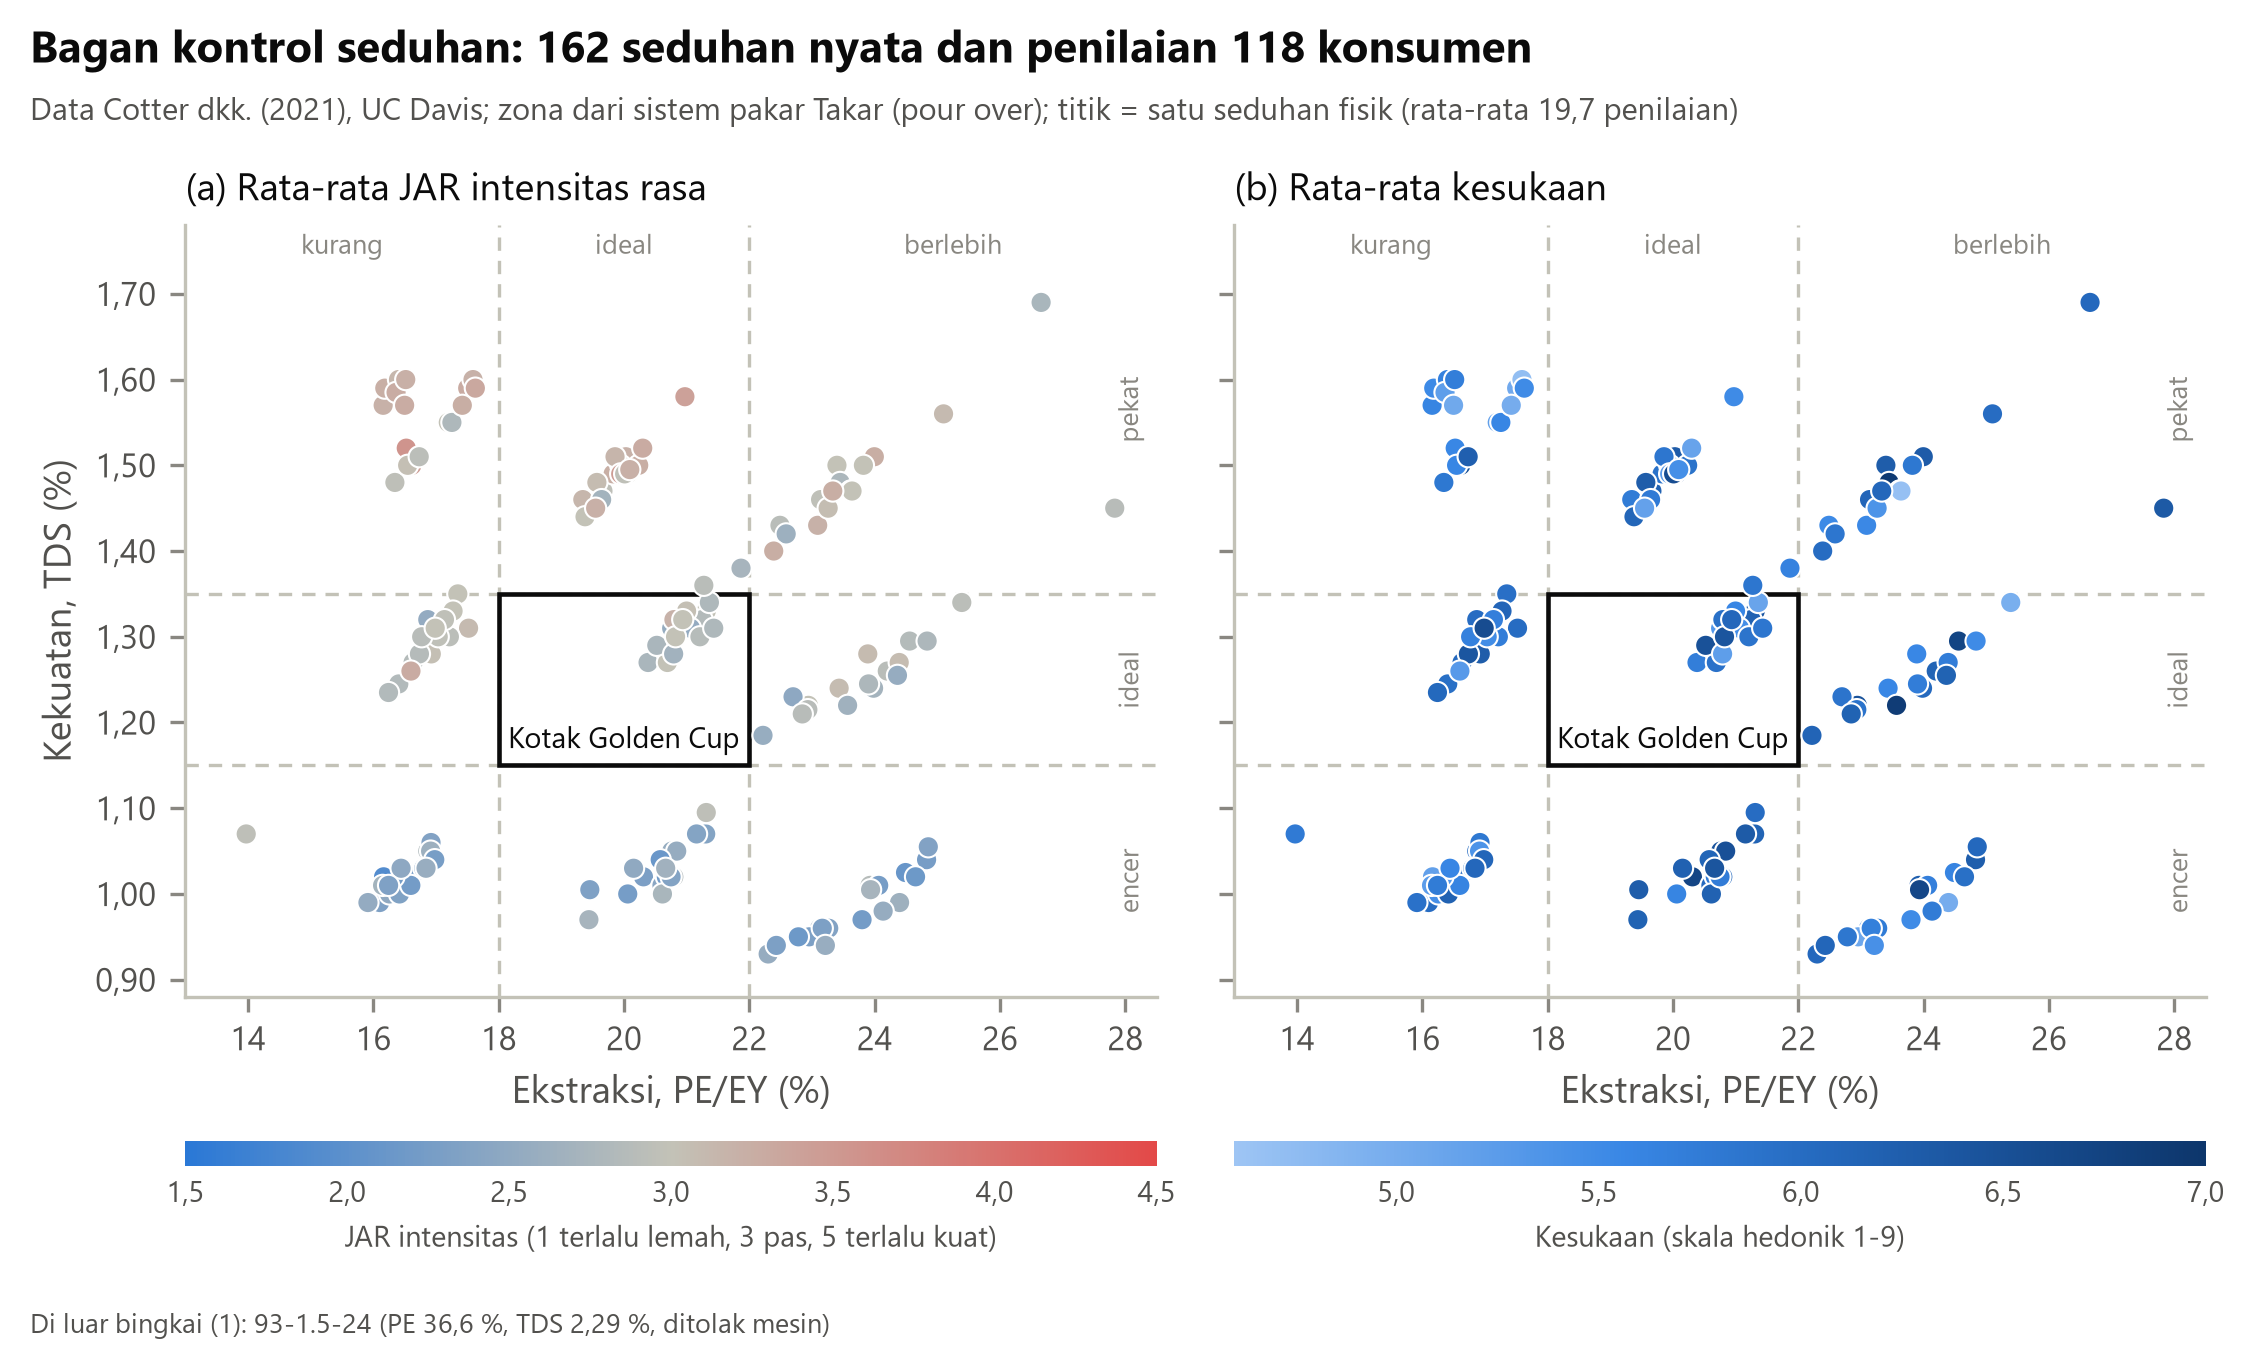
\includegraphics[width=.82\textwidth]{pic/results/figures/external_E4_control_chart.png}
\caption{Sebaran Seduhan Nyata pada Bagan Kendali Seduh}
\label{fig:hasil-kendali-seduh}
\end{figure}

\section{Hasil Evaluasi Asisten Barista AI}
\label{sec:hasil-asisten}

% sumber: results/assistant_eval.json (gabungan 420 jawaban, penilai versi 2.1).
Tolok ukur internal memuat 60 pertanyaan yang dibagi menjadi 14 fakta resep, 12 prosedur/SOP, 10 perhitungan, delapan diagnosis, enam stok, dan 10 pertanyaan di luar cakupan. Empat kondisi yang ditetapkan pada Bab~\ref{bab:metode} menghasilkan tujuh varian karena pencarian BM25 tidak memerlukan model dan tiga kondisi lain dijalankan pada Gemma 4 E4B serta E2B; totalnya 420 jawaban. Setelah kegagalan pemilihan alat pada percobaan awal ditemukan, hanya 120 jawaban kondisi RAG dengan alat dijalankan ulang pada router yang diperbaiki. Penggabungan dengan 300 jawaban kondisi lain memeriksa kesamaan hash tolok ukur dan basis data, lalu seluruh jawaban dinilai ulang oleh penilai versi 2.1. Suhu model ditetapkan nol dan \textit{seed} 42. Tabel~\ref{tab:hasil-asisten} melaporkan akurasi isi pada pertanyaan yang sama, akurasi yang juga mensyaratkan pemilihan alat dan argumen benar, serta latensi median seluruh pipeline.

\begin{table}[htbp]
\centering
\caption{Hasil Tolok Ukur Internal Asisten pada 60 Pertanyaan per Varian}
\label{tab:hasil-asisten}
\small
\begin{tabular}{llrrrr}
\toprule
Kondisi & Model & \shortstack{Akurasi\\isi (\%)} & \shortstack{Terverifikasi\\alat (\%)} & \shortstack{Mode\\LLM} & \shortstack{Latensi\\p50 (detik)} \\
\midrule
BM25 saja & -- & 55,0 & 55,0 & 0 & 0,027 \\
Tanpa konteks & E4B & 15,0 & 10,0 & 60 & 8,123 \\
RAG & E4B & 55,0 & 55,0 & 48 & 1,721 \\
RAG + alat & E4B & 95,0 & 95,0 & 26 & 0,175 \\
Tanpa konteks & E2B & 6,7 & 6,7 & 60 & 4,930 \\
RAG & E2B & 53,3 & 53,3 & 47 & 1,160 \\
RAG + alat & E2B & 93,3 & 93,3 & 26 & 0,150 \\
\bottomrule
\end{tabular}
\end{table}

Pencarian BM25 menempatkan rujukan benar pada peringkat pertama dalam 73,81\% dari 42 pertanyaan yang memiliki rujukan, pada tiga teratas dalam 85,71\%, dan pada lima teratas dalam 88,10\%; MRR-nya 0,7944. Akurasi pencarian saja 55,0\% pada seluruh 60 pertanyaan sudah mencakup penolakan pertanyaan di luar cakupan oleh gerbang aturan. Tabel~\ref{tab:hasil-asisten-kategori} menunjukkan bagian yang menyumbang perubahan E4B. Fakta resep sudah benar 14/14 pada RAG tanpa alat, sedangkan prosedur benar 9/12; keduanya tidak berubah setelah alat ditambahkan. Perhitungan, diagnosis, dan stok yang memerlukan layanan aplikasi berubah dari 0/24 menjadi 24/24 setelah router deterministik mengirim pertanyaan yang berparameter cukup ke alat yang tepat. Keberhasilan ini berasal dari layanan takaran, sistem pakar, inventaris, dan pasangan menu beserta routing-nya, bukan dari peningkatan kemampuan bahasa Gemma 4.

\begin{table}[htbp]
\centering
\caption{Akurasi Isi Gemma 4 E4B Menurut Jenis Pertanyaan}
\label{tab:hasil-asisten-kategori}
\small
\begin{tabular}{lrrrr}
\toprule
Jenis pertanyaan & Jumlah & Tanpa konteks (\%) & RAG (\%) & RAG + alat (\%) \\
\midrule
Fakta resep & 14 & 28,6 & 100,0 & 100,0 \\
Prosedur/SOP & 12 & 16,7 & 75,0 & 75,0 \\
Perhitungan & 10 & 0,0 & 0,0 & 100,0 \\
Diagnosis & 8 & 37,5 & 0,0 & 100,0 \\
Stok & 6 & 0,0 & 0,0 & 100,0 \\
Di luar cakupan & 10 & 0,0 & 100,0 & 100,0 \\
\bottomrule
\end{tabular}
\end{table}

Pada kondisi RAG dengan alat E4B, 24 jawaban memakai alat, 26 dijawab model, dan 10 ditolak gerbang cakupan sebelum model dipanggil. Ketepatan pemilihan alat dan argumen tercatat 100\% pada butir yang relevan. Dari 26 jawaban mode model, 23 benar (88,5\%); akurasi ini bersyarat pada pertanyaan yang diarahkan ke model dan tidak dapat dibandingkan langsung dengan 15,0\% tanpa konteks pada seluruh 60 pertanyaan. Median latensi seluruh pipeline 0,175 detik karena 34 jawaban melewati pemanggilan model; median untuk 26 jawaban model saja adalah 1,679 detik. Persentil ke-95 seluruh pipeline adalah 2,316 detik. Sepuluh jawaban yang tercatat sebagai mode pencarian pada varian ini semuanya adalah penolakan luar cakupan oleh gerbang aturan, bukan timeout. Pada RAG tanpa alat E4B terdapat 12 mode pencarian: 10 dari gerbang cakupan dan dua dari kegagalan runtime atau penjaga jawaban.

Tingkat angka tanpa dasar pada E4B tanpa konteks adalah 466 dari 542 angka jawaban (85,98\%), sedangkan pada E4B RAG dengan alat nol dari 263 angka jawaban (0\%). E2B menunjukkan pola serupa: 540 dari 659 angka tanpa dasar pada kondisi tanpa konteks (81,94\%) dan nol dari 255 pada RAG dengan alat. Penilai mencocokkan angka dengan pertanyaan, potongan dokumen yang benar-benar diberikan, atau keluaran alat, serta mengizinkan pembulatan hasil alat sesuai ketelitian tampilan. Angka nol berarti tidak ditemukan angka tanpa dukungan menurut pemeriksaan ini; nilai tersebut tidak membuktikan seluruh kalimat benar secara semantik. Pada model utama E4B, akurasi isi 95,0\% lebih tinggi daripada 15,0\% tanpa konteks dan tingkat angka tanpa dasar 0\% lebih rendah daripada 85,98\%, sehingga kedua syarat H5 terpenuhi pada tolok ukur internal. E2B memberi hasil searah, 93,3\% berbanding 6,7\% dan 0\% berbanding 81,94\%.

Interpretasi H5 dibatasi oleh rancangan sistem dan proses pengembangan. Router alat menghasilkan seluruh 24 jawaban pada butir perhitungan, diagnosis, dan stok; 10 penolakan luar cakupan terjadi sebelum model; hanya 26 butir fakta dan SOP melewati model E4B, dengan tiga kesalahan semuanya pada prosedur. Hasil 95,0\% adalah kinerja pipeline lengkap yang diuji ulang setelah routing disempurnakan memakai kegagalan pada tolok ukur yang sama. Butir disusun dengan bantuan AI, diperiksa terhadap sumber secara mesin, dan belum ditinjau manual oleh peneliti atau barista praktik. Karena itu, H5 didukung sebagai hasil uji regresi internal, bukan bukti bahwa Gemma 4 sendiri mencapai 95,0\% atau bahwa akurasi akan sama pada pertanyaan kedai baru.

\section{Kinerja Sistem}
\label{sec:hasil-kinerja}

% sumber: results/api_latency.json; results/lighthouse/summary.json
Pengukuran lokal memakai 20 permintaan pemanasan dan 200 permintaan berurutan per \textit{endpoint}. Median/persentil ke-95 kalkulator adalah 7,393/8,669~ms, daftar resep 9,174/11,460~ms, rekomendasi pasangan 3,635/4,402~ms, dan login 45,005/50,977~ms. Layanan \textit{restock} lebih berat dengan 137,741/159,285~ms; beranda yang merangkum beberapa sumber 146,838/182,477~ms. Angka ini dihitung pada komputer pengembangan dengan basis data salinan dan permintaan tanpa beban serentak, sehingga tidak mewakili latensi jaringan kedai atau banyak pengguna pada saat bersamaan.

Audit Lighthouse tiga kali pada halaman masuk memperoleh median skor kinerja 1,00 untuk desktop dan 0,97 untuk ponsel; skor aksesibilitas dan praktik terbaik pada kedua preset 1,00. Audit hanya mencakup halaman publik, bukan halaman setelah masuk. Hasilnya juga bergantung pada versi Chrome dan simulasi perangkat saat pengukuran.

\section{Pengujian Penerimaan Pengguna}
\label{sec:hasil-uat}

Instrumen tugas dan kuesioner SUS dicantumkan pada lampiran. Belum ada catatan sesi dengan barista atau pengelola kedai mitra, jumlah peserta, tingkat penyelesaian tugas, maupun skor SUS. Karena itu, kelayakan penggunaan dalam lingkungan kerja belum dapat disimpulkan dari pengujian otomatis saja.

\section{Pembahasan}
\label{sec:pembahasan}

H1 didukung pada pesanan yang tercakup grid karena aturan diskret dan ruang cangkir menghilangkan pelanggaran yang timbul dari penskalaan linier. Namun, peringatan kurang isi pada 144 pesanan memperlihatkan kebutuhan aturan keputusan tambahan: barista mungkin perlu mengganti ukuran, menurunkan jumlah \textit{shot}, atau menolak kombinasi tertentu. Validasi menu Starbucks memperlihatkan bahwa \textit{shot} utuh saja belum cukup untuk meniru standar satu jaringan; pengecualian ukuran diperlukan dan kecocokan 100\% yang memakai tabel menu sendiri tidak boleh disebut kemampuan prediksi.

H2 menunjukkan ketergantungan kuat pada sifat keranjang. Pada sampel fiktif IBM, FP-Growth jauh di atas popularitas, tetapi pada transaksi nyata Bread Basket selisih HR@5 tidak meyakinkan dan urutan peringkatnya bahkan lebih buruk. Ko-okurensi sederhana unggul pada dua data yang dilaporkan. Saringan \textit{lift} lebih dari satu menjaga asosiasi yang kuat relatif terhadap kebetulan, tetapi dapat membuang pasangan yang relevan secara operasional ketika salah satu item sangat populer. Sebelum diterapkan pada transaksi kedai nyata, kebijakan saringan dan pembanding perlu dinilai ulang pada data kedai tersebut.

H3 tidak berpindah dengan baik dari Maven ke ihelon. Perbedaan bentuk data, volume, dan konteks mesin penjual kopi dapat mengubah model yang paling sesuai. Memilih ulang model pada jendela ihelon yang sama akan memberi hasil optimistis; karena itu keputusan H3 mempertahankan model yang dipilih sebelumnya. H4 tetap didukung pada simulasi ihelon, tetapi analisis kontrol menunjukkan bahwa kebijakan tingkat sasaran dinamis dan asumsi pasokan menjelaskan sebagian manfaat, sedangkan model global bukan peramal terbaik di sana. Hal ini membatasi klaim AI dari ``model terbaik'' menjadi prosedur yang dapat diuji dan disesuaikan.

Untuk asisten tanya-jawab, batas validasi berbeda dari modul transaksi. Enam puluh butir tolok ukur disusun dengan bantuan AI dan diperiksa secara mesin, tetapi belum ditinjau barista independen. Kegagalan awal pada butir yang sama juga memandu penyempurnaan router alat sebelum pengujian akhir. Karena itu, perbandingan akhir mengukur regresi pipeline pada tolok ukur internal yang telah memengaruhi pengembangan, bukan generalisasi pada pertanyaan baru. Empat kueri tambahan dipakai sebagai pemeriksaan cepat, tetapi belum merupakan himpunan uji acak yang divalidasi manusia. Selain itu, penolakan pertanyaan di luar cakupan berasal dari gerbang aturan yang bekerja sebelum model; jawaban mode alat berasal dari layanan aplikasi; dan jawaban mode pencarian dapat muncul ketika model tidak tersedia atau keluaran tidak lolos penjaga. Ketiga mekanisme tersebut harus dibedakan ketika menafsirkan akurasi keseluruhan.

Pengujian sistem pakar membenarkan perhitungan EY dan memberi sebagian kesesuaian arah kekuatan terhadap penilaian konsumen, tetapi kotak teknis tidak mengungguli area luarnya dalam rata-rata kesukaan. Sistem lebih tepat dipakai sebagai alat bantu diagnosis yang menunjukkan alasan daripada penentu rasa ideal tunggal. H5 terpenuhi dalam uji regresi asisten yang mencakup router, model, alat, penjaga, dan gerbang cakupan, tetapi tolok ukur yang memandu perbaikan tersebut belum menjadi validasi independen. Batas keseluruhan penelitian juga mencakup data pengembangan fiktif, pemetaan BOM dan parameter pasokan asumtif, keterwakilan validasi eksternal yang terbatas, dan belum adanya UAT. Kesimpulan pada Bab~\ref{bab:simpulan} mengikuti batas tersebut.


% % Bab 5 : Kesimpulan dan Saran
\chapter{\babLima}
\label{bab:simpulan}
% Keputusan H1--H4 merujuk results/scaling_eval.json, pairing_eval.json,
% forecast_eval.json, restock_eval.json, dan results/external/E1--E5*.json.
% Keputusan H5 merujuk results/assistant_eval.json (penilai versi 2.1).

\section{Simpulan}
\label{sec:simpulan}

Penelitian ini menghasilkan Takar, aplikasi web yang menghubungkan resep standar, SOP, perhitungan variasi pesanan, panduan seduh beranimasi, pencatatan produksi, dan buku besar persediaan. Resep menyimpan ukuran, komponen, aturan takaran, parameter mutu, dan langkah seduh; produksi yang dicatat diuraikan menjadi pemakaian bahan berdasarkan BOM. Hak pengguna dibedakan antara manajer, kepala barista, dan barista. Sebanyak 706 uji backend dan 29 kasus antarmuka otomatis lulus. Hasil tersebut menjawab kebutuhan integrasi pada rumusan masalah pertama dari sisi implementasi, tetapi belum mengukur perubahan konsistensi rasa atau lama pelatihan staf di kedai nyata.

Untuk rumusan masalah kedua, penskalaan berbasis batasan memenuhi kriteria H1 pada 525 variasi pesanan yang diuji: tidak ada \textit{shot} pecahan, luapan cangkir lebih dari 5\%, atau penyimpangan rasio lebih dari 0,2. Pembanding linier mentah menghasilkan 240 pesanan dengan \textit{shot} pecahan dan 267 luapan; pembanding linier yang dibulatkan tetap menghasilkan 282 luapan. Sebagian hasil nol melekat pada bentuk algoritma, sehingga ditandai \textit{by construction}. Sebanyak 144 pesanan masih mendapat peringatan kurang isi, yang menuntut keputusan operasional lebih lanjut. Validasi menu Starbucks menunjukkan aturan \textit{shot} utuh berguna, tetapi tabel pengecualian ukuran dibutuhkan untuk merepresentasikan pola kedai tertentu; kecocokan sempurna ketika tabel diisi dari menu yang sama bukan bukti kemampuan prediksi.

Untuk rekomendasi pasangan menu, H2 didukung pada data pengembangan IBM yang bersifat fiktif, tetapi tidak didukung pada transaksi nyata Bread Basket: selisih HR@5 FP-Growth terhadap popularitas sebesar 0,0060 mempunyai IK 95\% [-0,0028; 0,0147]. Pembanding ko-okurensi juga lebih tinggi daripada FP-Growth pada HR@5 data nyata tersebut. Hasil ini menunjukkan bahwa saringan \textit{lift} aplikasi perlu diuji lagi pada transaksi kedai tujuan sebelum dipakai sebagai dasar penawaran menu.

Pada peramalan, model \textit{gradient boosting} global mempunyai WAPE terendah pada data pengembangan Maven, tetapi H3 tidak didukung pada ihelon. WAPE per minumannya sedikit lebih rendah daripada \textit{seasonal naive} tanpa selisih yang meyakinkan, sedangkan WAPE total harian justru lebih tinggi. H4 didukung untuk kebijakan pengisian ulang berbasis prakiraan dibandingkan ROP statis pada simulasi ihelon, dengan \textit{fill rate} rata-rata 0,9605 berbanding 0,7900. Analisis kontrol menunjukkan bahwa struktur tingkat sasaran dinamis berperan penting dan model global bukan peramal terbaik dalam replay itu. Oleh karena itu, hasil simulasi tidak boleh ditafsirkan sebagai bukti bahwa satu model AI selalu memberi stok terbaik.

Sistem pakar mereproduksi perhitungan EY pada seduhan dengan massa terukur dan memperlihatkan kesesuaian arah kekuatan terhadap sebagian penilaian konsumen. Akan tetapi, kesukaan rata-rata di dalam kotak \textit{Golden Cup} tidak lebih tinggi secara meyakinkan daripada di luar kotak. Diagnosis harus dibaca sebagai bantuan yang menjelaskan alasan teknis, bukan penilaian tunggal atas preferensi pelanggan.

H5 didukung secara deskriptif pada tolok ukur internal: akurasi isi asisten E4B dengan RAG dan alat 95,0\% berbanding 15,0\% tanpa konteks, sedangkan tingkat angka tanpa dasar 0\% berbanding 85,98\% menurut penilai versi 2.1. Pada kondisi lengkap, 24 jawaban berasal dari router dan alat deterministik, 10 penolakan luar cakupan dari gerbang aturan, dan 26 jawaban dari model, sehingga hasil keseluruhan tidak menyatakan akurasi Gemma 4 sendiri. Tiga jawaban E4B yang salah seluruhnya terkait prosedur/SOP. Karena butir disusun dengan bantuan AI, belum ditinjau barista praktik, dan telah dipakai untuk memperbaiki router sebelum uji akhir, angka 95,0\% merupakan hasil regresi internal, bukan estimasi generalisasi pada kedai baru. Dengan batas itu, rumusan masalah ketiga terjawab sebagai perbandingan terukur antarmodul dan kondisi, bukan pembuktian manfaat operasional pada pengguna nyata.

Kelayakan fungsional awal didukung oleh pengujian otomatis dan pengukuran kinerja lokal, tetapi rumusan masalah keempat belum sepenuhnya terjawab. Uji penerimaan pengguna bersama barista atau pengelola dan skor SUS belum tersedia. Kesimpulan tentang kemudahan pakai, pengurangan waktu pelatihan, pengurangan limbah, maupun keuntungan usaha memerlukan pengamatan pada kedai mitra, bukan hanya hasil dataset publik dan simulasi.

\section{Saran}
\label{sec:saran}

Penerapan berikutnya sebaiknya dimulai dengan mengukur resep dan ukuran cangkir di kedai mitra, memvalidasi takaran pengisi dan ambang kurang isi bersama kepala barista, lalu mencatat produksi serta stok aktual beberapa minggu. Parameter \textit{lead time}, kemasan, kehilangan bahan, dan stok awal perlu diambil dari pemasok dan buku stok nyata. Dengan demikian, saran pemesanan ulang dapat dihitung dari kondisi yang benar-benar dihadapi kedai, bukan dari data contoh.

Model pasangan menu dan peramalan perlu dilatih serta dinilai ulang pada transaksi kedai tujuan memakai pemisahan waktu. Ko-okurensi dan model musiman sederhana harus tetap menjadi pembanding karena keduanya unggul pada sebagian validasi eksternal. Kebijakan \textit{restock} perlu dievaluasi bersama biaya pemesanan, ruang penyimpanan, masa simpan susu dan bahan lain, serta barang yang sedang dipesan. Pengembangan lanjutan dapat menambahkan pencatatan pesanan pembelian dan integrasi kasir setelah alur satu outlet stabil.

Asisten lokal perlu diaudit dengan himpunan pertanyaan baru yang disusun dan diperiksa barista independen, khususnya angka takaran, saran koreksi, pertanyaan di luar cakupan, dan sumber jawaban. Himpunan itu harus dipisahkan dari butir yang telah memandu penyempurnaan router alat agar ketepatan pada kasus baru dapat diukur. Ketepatan alat, jawaban model, hasil pencarian cadangan, dan penolakan oleh aturan perlu dilaporkan terpisah. Hasil model dan aturan pakar harus ditinjau saat resep atau SOP berubah. Akhirnya, uji tugas barista dan SUS perlu dilaksanakan dengan peserta, perangkat, dan kondisi kerja yang dicatat jelas; hasilnya kemudian dipakai untuk memperbaiki navigasi, istilah, serta alur produksi sebelum klaim manfaat operasional dibuat.



%
% Daftar Pustaka
\renewcommand\bibname{REFERENSI}
\bibliographystyle{apacite}
\bibliography{ref}
%\includepdf[page=-,pagecommand={},width=\textwidth]{loogbook4}

% Dari sini
% % Lampiran 
% \begin{appendix}
% 	\pagenumbering{gobble}
% 	%
% 
% Hanya sebuah pembatas bertuliskan LAMPIRAN ditengah halaman. 
% 

\begin{titlepage}
	\centering 
	\vspace*{6cm}
	\noindent \Huge{LAMPIRAN}
	\addChapter{LAMPIRAN}
\end{titlepage}


% 	\setcounter{page}{2}
% \end{appendix}

\clearpage
\chapter*{LAMPIRAN}
\phantomsection
\addcontentsline{toc}{chapter}{LAMPIRAN}
\setcounter{table}{0}
\renewcommand{\thetable}{L.\arabic{table}}
\setcounter{figure}{0}
\renewcommand{\thefigure}{L.\arabic{figure}}
% Lampiran adalah ringkasan yang dapat ditelusuri ke berkas proyek. Data hasil tidak
% disalin atau dibuat ulang di sini. Instrumen UAT belum diisi oleh peserta.

\section*{Lampiran A. Basis Pengetahuan Resep dan Asumsi}
\phantomsection
\addcontentsline{toc}{section}{Lampiran A. Basis Pengetahuan Resep dan Asumsi}

Arahan pembimbing menjadi sumber tujuh kelompok resep pada Tabel~\ref{tab:lampiran-resep}. Nama, langkah, dan angka asli disimpan bersama penanda \texttt{source=pdf\_arahan} di \path{app/backend/app/seed/recipes.json} dan SOP terkait. Ringkasan ini dipakai untuk mengaudit hubungan antara arahan, resep digital, dan uji kalkulator; berkas JSON merupakan daftar terperinci yang dijalankan aplikasi.

\begin{table}[htbp]
\centering
\caption{Ringkasan Angka Resep dari Arahan Pembimbing}
\label{tab:lampiran-resep}
\small
\begin{tabular}{>{\RaggedRight\arraybackslash}p{.26\textwidth}>{\RaggedRight\arraybackslash}p{.61\textwidth}}
\toprule
Resep & Fakta dalam arahan \\
\midrule
Caffè Latte panas & Satu \textit{shot} espreso ganda, susu segar dengan \textit{microfoam} tipis sekitar 1~cm, cangkir 200--250~ml; susu 60--65~$^\circ$C. \\
Cappuccino panas & Satu \textit{shot} espreso, susu panas dengan busa tebal sekitar 1,5--2~cm; cangkir 150--180~ml. \\
Ice Brown Sugar Shaken Espresso & Dua \textit{shot} espreso, 20~ml sirup gula aren, es secukupnya, dan susu segar sebagai pengisi. \\
Americano/Long Black & Dua \textit{shot} espreso dan air mineral atau es; Long Black menuangkan air lebih dulu, Americano espreso lebih dulu. \\
V60/\textit{Pour Over} & Kopi 15~g dan air 225~ml (1:15), air 90--92~$^\circ$C. \textit{Bloom} 45~ml selama 30--45 detik, target 130~ml pada menit 1:00 dan 225~ml pada menit 1:30; selesai 2:30--3:00. \\
Iced Matchagato/Matcha Latte Creamy & Matcha 5~g, air hangat 15~ml, sirup sederhana 15~ml, susu segar 150~ml, dan es; matcha dilarutkan lebih dulu. \\
Signature Pandan Latte & Satu \textit{shot} espreso, ekstrak pandan 20~ml, susu segar 150~ml, dan es; sirup pandan berada di dasar, espreso di atas. \\
\bottomrule
\end{tabular}
\end{table}

Angka yang tidak berasal dari arahan dicatat di \path{app/backend/app/seed/ASSUMPTIONS.md} dengan kode A01--A25. Tabel~\ref{tab:lampiran-asumsi} menyajikan asumsi yang paling berpengaruh pada hasil. Seluruh stok awal, waktu pasok, ukuran kemasan, dan jumlah pesan adalah data contoh; pembaca dapat menggantinya dengan hasil pengamatan kedai tanpa mengubah fakta resep yang berasal dari arahan.

\begin{table}[htbp]
\centering
\caption{Asumsi Utama Implementasi dan Dampaknya}
\label{tab:lampiran-asumsi}
\begin{tabular}{lp{.34\textwidth}p{.39\textwidth}}
\toprule
Kode & Isi & Dampak \\
\midrule
A01--A03 & Arti \textit{shot} ganda dan parameter espreso tambahan. & Kebutuhan biji dan volume komponen. \\
A04--A06 & Ukuran cangkir, ekspansi susu, massa jenis es. & Sisa ruang dan takaran pengisi. \\
A09--A10 & Ketelitian takar dan batas kurang isi. & Pembulatan dan peringatan kalkulator. \\
A11--A14 & Dosis V60 dan batas kemanisan. & Variasi pesanan yang dapat diproses. \\
A16, A24 & Stok, \textit{lead time}, kemasan, parameter simulasi. & Status serta kuantitas \textit{restock}. \\
A25 & Batas kewajaran masukan seduh. & Input yang diterima sistem pakar. \\
\bottomrule
\end{tabular}
\end{table}

\section*{Lampiran B. Pemetaan Produk dan Aturan AI}
\phantomsection
\addcontentsline{toc}{section}{Lampiran B. Pemetaan Produk dan Aturan AI}

Pemetaan lengkap antara produk IBM/Maven dan resep disimpan sebagai \path{app/backend/app/seed/product_recipe_map.json}; penjelasan asumsi ukuran dan proksi berada pada \path{ASSUMPTIONS.md}. Produk Latte dipetakan ke Caffè Latte, Cappuccino ke resep Cappuccino, minuman espreso ke subresep espreso, dan seduhan filter ke V60. Cokelat panas, chai, serta teh menggunakan resep tambahan yang nilainya dinyatakan asumsi. Roti dan barang kemasan tidak diuraikan ke bahan resep. Nama produk yang dipakai untuk pasangan menu dinormalisasi ke kunci tanpa ukuran, sedangkan pemetaan ke resep dipakai saat ramalan penjualan diubah menjadi kebutuhan bahan.

Basis pengetahuan koreksi seduh tersimpan pada \path{app/backend/app/ai/kb/brew_rules.json}. Setiap aturan memuat kondisi, fakta yang disimpulkan, prioritas, saran, dan sumber. Jejak aturan dikembalikan kepada pengguna agar diagnosis dapat diperiksa. Hasil evaluasi E4 menunjukkan mengapa jejak itu diperlukan: arah kekuatan hanya cocok dengan sebagian penilaian konsumen, dan preferensi kesukaan tidak sama dengan berada di kotak teknis \textit{Golden Cup}. Daftar aturan lengkap lebih tepat dibaca dari berkas JSON yang digunakan mesin daripada ditranskripsi ulang ke naskah.

\section*{Lampiran C. Ringkasan Kasus Pengujian Otomatis}
\phantomsection
\addcontentsline{toc}{section}{Lampiran C. Ringkasan Kasus Pengujian Otomatis}

Kasus \textit{black-box} antarmuka terperinci berada di \path{app/results/tests/blackbox_cases.csv}. Berkas itu memuat identitas, langkah, hasil yang diharapkan, hasil aktual, dan status otomatis. Tabel~\ref{tab:lampiran-kasus} memudahkan pencarian kelompok kasus; bukti tangkapan layar berada di \path{app/results/screenshots/blackbox}. Jumlah lulus pada Bab~\ref{bab:hasil} mengacu pada berkas yang diregenerasi setelah perubahan kode terakhir.

\begin{table}[htbp]
\centering
\caption{Cakupan Kasus \textit{Black-Box} Antarmuka}
\label{tab:lampiran-kasus}
\begin{tabular}{lp{.69\textwidth}}
\toprule
ID & Cakupan \\
\midrule
BB-01--BB-04 & Masuk tiga peran, navigasi berizin, dan kata sandi keliru. \\
BB-05--BB-08 & Katalog dan detail resep, ukuran latte, kalkulator V60. \\
BB-09--BB-10 & Pencatatan produksi, pengurangan stok, penerimaan dan opname. \\
BB-11--BB-14 & Checklist SOP, panduan V60, timer espreso, diagnosis seduh. \\
BB-15--BB-18 & \textit{Restock}, prakiraan, pasangan menu, dan metrik evaluasi AI. \\
BB-19--BB-22 & Akun pengguna, data/model, keluar, dan navigasi ponsel. \\
BB-23--BB-26 & Perubahan resep/SOP, detail V60, dan ringkasan beranda. \\
BB-27 & Asisten AI menampilkan jawaban V60 yang relevan dan rujukan resep/SOP. \\
BB-28 & Animasi Panduan Seduh menampilkan tindakan, waktu, dan target sesuai tahap resep aktif. \\
BB-29 & Tautan saran pasangan menu membuka Panduan Seduh pada resep yang cocok. \\
\bottomrule
\end{tabular}
\end{table}

\section*{Lampiran D. Instrumen Uji Penerimaan Pengguna}
\phantomsection
\addcontentsline{toc}{section}{Lampiran D. Instrumen Uji Penerimaan Pengguna}

Instrumen ini disiapkan untuk sesi barista dan pengelola kedai; belum ada responden atau skor yang diisi. Sebelum sesi, peneliti mencatat kode peserta tanpa nama di lembar analisis, peran pekerjaan, pengalaman meracik kopi, perangkat, tanggal, dan versi aplikasi. Peserta diberi akun sesuai peran dan diminta mengerjakan tugas tanpa demonstrasi penyelesaian. Peneliti mencatat keberhasilan, waktu, bantuan yang diberikan, dan masalah yang teramati. Kata sandi demo diganti sebelum pengujian di lingkungan bersama.

\begin{table}[H]
\centering
\caption{Tugas UAT dan Kriteria Keberhasilan}
\label{tab:lampiran-uat}
\small
\begin{tabular}{l>{\RaggedRight\arraybackslash}p{.49\textwidth}>{\RaggedRight\arraybackslash}p{.32\textwidth}}
\toprule
ID & Tugas peserta & Kriteria keberhasilan \\
\midrule
U1 & Temukan resep Caffè Latte dan jelaskan takaran serta suhu susu. & Halaman resep tepat; informasi standar ditemukan. \\
U2 & Hitung tiga Caffè Latte ukuran besar dengan tambahan satu \textit{shot}. & Takaran per cangkir, total, dan peringatan terbaca. \\
U3 & Hitung V60 dosis 20~g dan temukan target tuang bertahap. & Air 300~ml dan target 60/173,3/300~ml ditemukan. \\
U4 & Jalankan panduan seduh dan timer sampai langkah berikutnya. & Timer serta target langkah dipakai dengan benar. \\
U5 & Catat satu produksi dan periksa perubahan stok bahan. & Log produksi dan mutasi stok yang sesuai ditemukan. \\
U6 & Kerjakan checklist pembukaan bar. & Langkah kritis ditandai dan status selesai tersimpan. \\
U7 & Temukan bahan yang perlu dipesan ulang dan jelaskan dasar sarannya. & Status, jumlah pesan, dan label data contoh dipahami. \\
U8 & Masukkan gejala seduhan dan baca alasan diagnosis. & Saran dan aturan yang terpenuhi ditemukan. \\
U9 & Ajukan pertanyaan resep kepada asisten AI lokal dan buka sumber jawabannya. & Jawaban, mode, dan rujukan yang relevan terbaca. \\
U10 & Pilih saran pasangan menu yang memiliki resep aktif, buka panduannya, lalu ikuti ilustrasi tahap seduh. & Tautan menuju resep benar; tindakan, waktu, dan target tahap dijelaskan sesuai panduan. \\
\bottomrule
\end{tabular}
\end{table}

Sesudah tugas, peserta mengisi 10 pernyataan SUS berikut dengan skala 1 = sangat tidak setuju sampai 5 = sangat setuju. Redaksi Bahasa Indonesia ini disiapkan sebagai instrumen penelitian, sehingga pemahaman istilah perlu diperiksa pada sesi percontohan. Butir ganjil bersifat positif dan butir genap negatif sesuai pola SUS \citep*{brooke1996sus}.

\begin{table}[H]
\centering
\caption{Kuesioner \textit{System Usability Scale} yang Disiapkan}
\label{tab:lampiran-sus}
\begin{tabular}{r>{\RaggedRight\arraybackslash}p{.76\textwidth}}
\toprule
No. & Pernyataan \\
\midrule
1 & Saya merasa akan sering menggunakan aplikasi ini. \\
2 & Saya merasa aplikasi ini terlalu rumit untuk digunakan. \\
3 & Saya merasa aplikasi ini mudah digunakan. \\
4 & Saya merasa memerlukan bantuan orang yang memahami teknis untuk menggunakan aplikasi ini. \\
5 & Saya merasa fungsi-fungsi dalam aplikasi ini terintegrasi dengan baik. \\
6 & Saya merasa terdapat terlalu banyak hal yang tidak konsisten dalam aplikasi ini. \\
7 & Saya membayangkan kebanyakan orang akan cepat belajar menggunakan aplikasi ini. \\
8 & Saya merasa aplikasi ini sangat merepotkan untuk digunakan. \\
9 & Saya merasa yakin ketika menggunakan aplikasi ini. \\
10 & Saya perlu mempelajari banyak hal sebelum dapat menggunakan aplikasi ini. \\
\bottomrule
\end{tabular}
\end{table}

Skor tiap butir ganjil dihitung sebagai jawaban dikurangi satu; butir genap sebagai lima dikurangi jawaban. Jumlah kontribusi sepuluh butir dikalikan 2,5 untuk memperoleh skor 0--100 per peserta. Rerata baru dihitung setelah jawaban nyata tersedia, disertai jumlah peserta dan sebarannya. Skor tidak boleh diisi dari perkiraan peneliti atau hasil pengujian otomatis.

\section*{Lampiran E. Reproduksi Hasil}
\phantomsection
\addcontentsline{toc}{section}{Lampiran E. Reproduksi Hasil}

Dataset yang diperlukan ditempatkan sesuai \path{dataset/raw/*/DATASHEET.md}. Dari folder \path{app}, instalasi dilakukan dengan \path{setup.bat}, lalu aplikasi dijalankan dengan \path{run.bat}. Untuk mengulang evaluasi, jalankan perintah berikut dari \path{app/backend} menggunakan lingkungan Python yang dibuat \path{setup.bat}. Setiap skrip menulis parameter, hash data, dan hasil baru ke \path{app/results}; keluaran lama tidak perlu disalin manual.

\begin{verbatim}
.venv\Scripts\python.exe scripts\evaluate_scaling.py
.venv\Scripts\python.exe scripts\evaluate_pairing.py
.venv\Scripts\python.exe scripts\evaluate_forecasting.py
.venv\Scripts\python.exe scripts\evaluate_restock.py
.venv\Scripts\python.exe scripts\evaluate_pairing_external.py
.venv\Scripts\python.exe scripts\evaluate_forecasting_external.py
.venv\Scripts\python.exe scripts\evaluate_restock_external.py
.venv\Scripts\python.exe scripts\validate_expert_system.py
.venv\Scripts\python.exe scripts\validate_scaling_starbucks.py
.venv\Scripts\python.exe scripts\check_external_results.py
.venv\Scripts\python.exe scripts\evaluate_assistant.py
.venv\Scripts\python.exe -m pytest -q
\end{verbatim}

Evaluasi asisten memerlukan Ollama dan kedua model Gemma 4 yang disebut pada Bab~\ref{bab:hasil}; skrip menjalankan tujuh varian pada 60 butir dan menyimpan jawaban beserta skor. Hasil yang dilaporkan menggabungkan 300 jawaban kondisi lama dengan 120 jawaban RAG dan alat setelah perbaikan router; prosesnya dapat diulang secara deterministik dari jawaban mentah yang disimpan dengan perintah berikut. Skrip penggabungan menolak hash tolok ukur atau basis data yang berbeda; skrip penilai ulang tidak memanggil model. Menjalankan evaluasi dari awal dapat menghasilkan jawaban berbeda karena perangkat dan runtime model dapat berubah.

\begin{verbatim}
.venv\Scripts\python.exe scripts\merge_assistant_eval.py
.venv\Scripts\python.exe scripts\rescore_assistant.py ^
  --input ..\results\assistant_eval_merged_raw.json ^
  --output-stem assistant_eval
\end{verbatim}

Tanda \texttt{\^{}} pada baris perintah di atas adalah penyambung baris Windows; kedua baris \texttt{rescore\_assistant.py} dapat pula ditulis dalam satu baris. Pengujian antarmuka dijalankan dari \path{app/frontend} dengan \texttt{npm run build}, \texttt{npm run test:e2e}, dan \texttt{npm run screenshots}. Pengukuran API memakai \path{scripts/measure_api_latency.py}; Lighthouse memakai \texttt{npm run lighthouse}. Waktu pengukuran latensi dan skor Lighthouse dapat berubah sesuai komputer serta beban saat pelaksanaan.

\section*{Lampiran F. Tampilan Panduan Seduh Beranimasi}
\phantomsection
\addcontentsline{toc}{section}{Lampiran F. Tampilan Panduan Seduh Beranimasi}

Gambar~\ref{fig:lampiran-animasi-v60} dan Gambar~\ref{fig:lampiran-animasi-espresso} memperlihatkan keadaan antarmuka ketika tahap resep ditampilkan. Gambar diam hanya mendokumentasikan satu posisi ilustrasi; gerak, jeda, dan pergantian tahap diperiksa melalui pengujian antarmuka BB-28. Gambar~\ref{fig:lampiran-pairing-panduan} memperlihatkan tautan panduan pada saran yang memiliki padanan resep aktif, sedangkan Gambar~\ref{fig:lampiran-pairing-mobile} menunjukkan tahap yang dibuka pada ponsel setelah tautan itu dipilih dalam BB-29. Gambar-gambar ini adalah bukti implementasi, bukan hasil pengukuran keberhasilan belajar pengguna.

\begin{figure}[htbp]
\centering
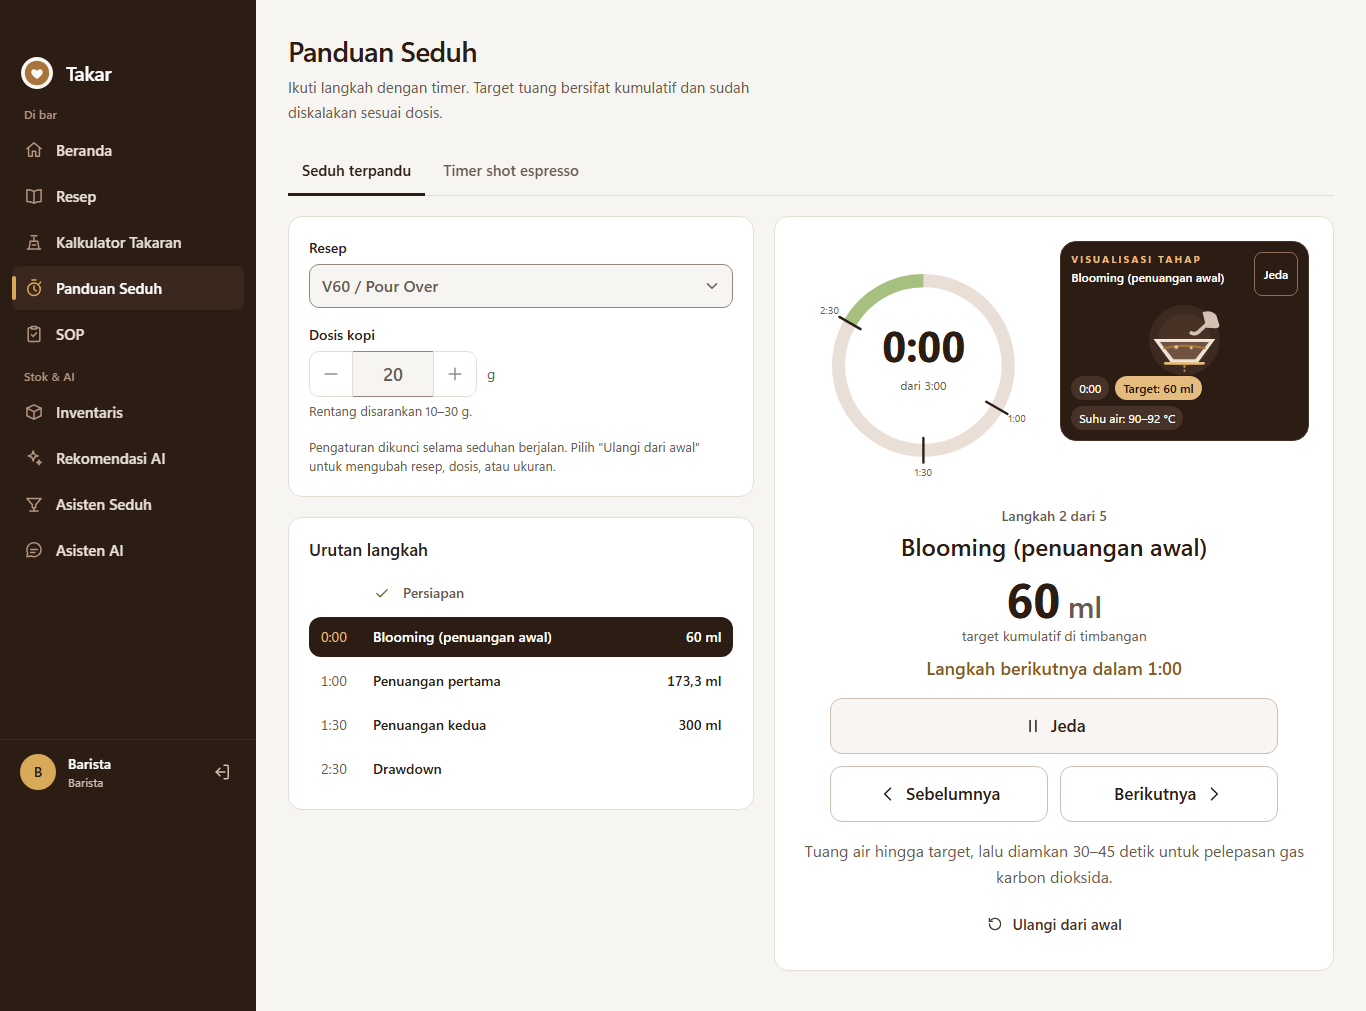
\includegraphics[width=.82\textwidth]{pic/results/screenshots/blackbox/BB-28-brew-animation.png}
\caption{Tahap \textit{blooming} V60 dosis 20~g dengan ilustrasi bergerak, timer aktif, dan target 60~ml}
\label{fig:lampiran-animasi-v60}
\end{figure}

\begin{figure}[htbp]
\centering
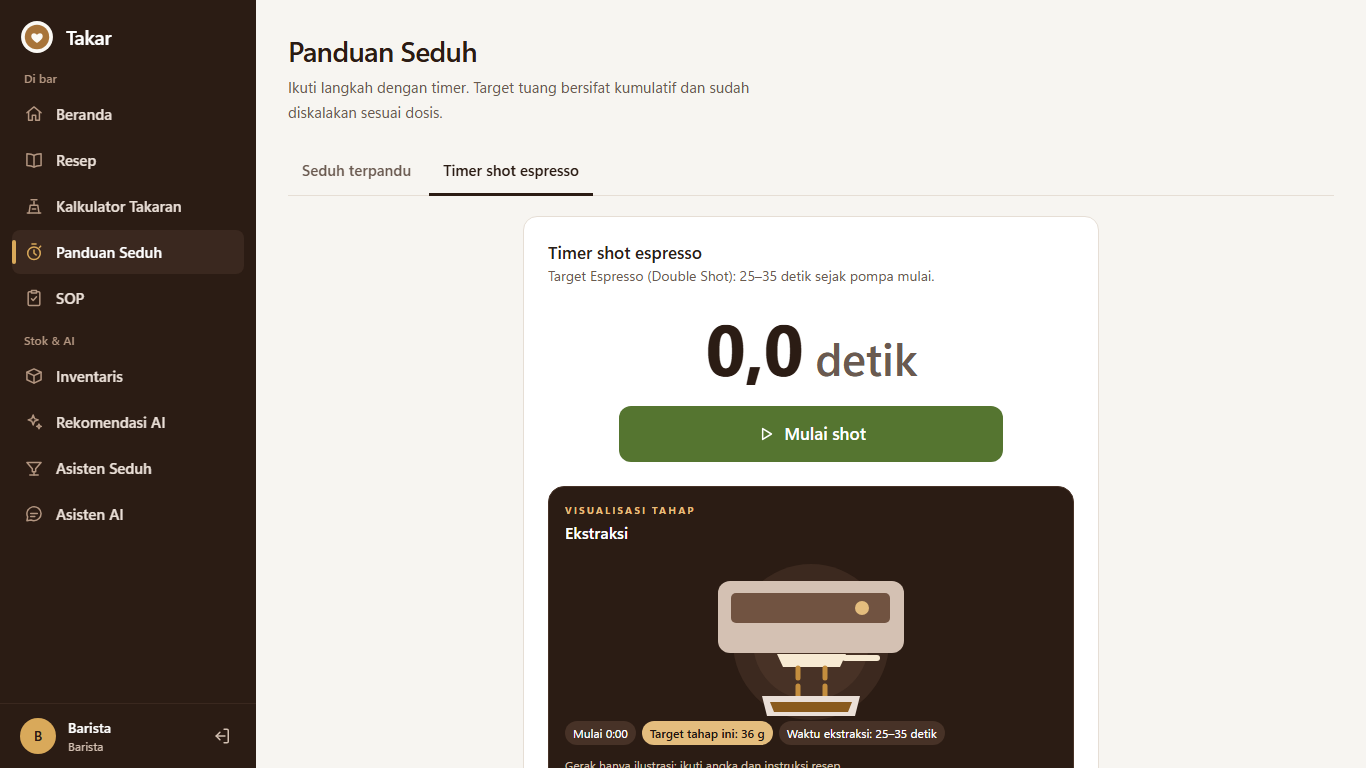
\includegraphics[width=.88\textwidth]{pic/results/screenshots/desktop/10-timer-shot-espresso.png}
\caption{Ilustrasi ekstraksi pada Timer Shot Espresso dengan target waktu dan hasil resep}
\label{fig:lampiran-animasi-espresso}
\end{figure}

\begin{figure}[htbp]
\centering
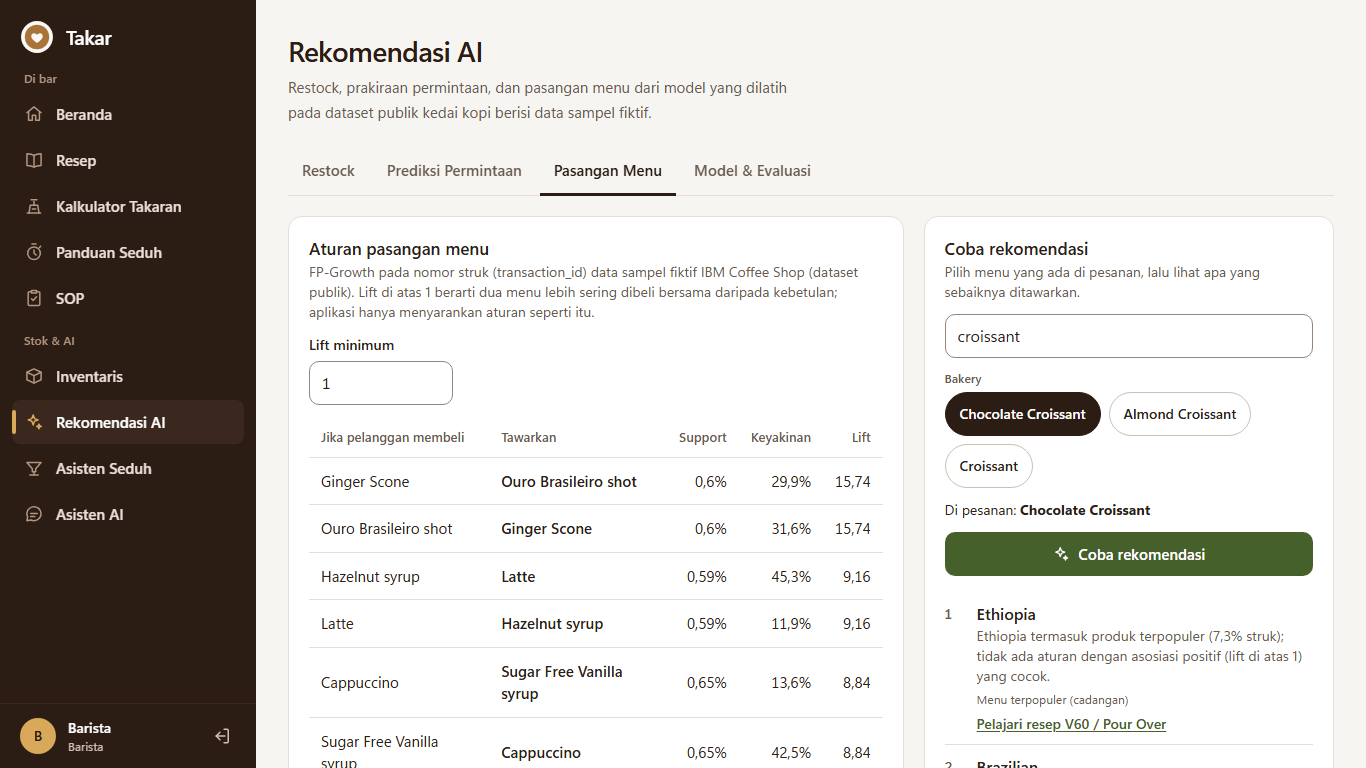
\includegraphics[width=.88\textwidth]{pic/results/screenshots/desktop/18-ai-pasangan-menu.png}
\caption{Tautan ``Pelajari resep V60 / Pour Over'' pada saran pasangan menu}
\label{fig:lampiran-pairing-panduan}
\end{figure}

\begin{figure}[htbp]
\centering
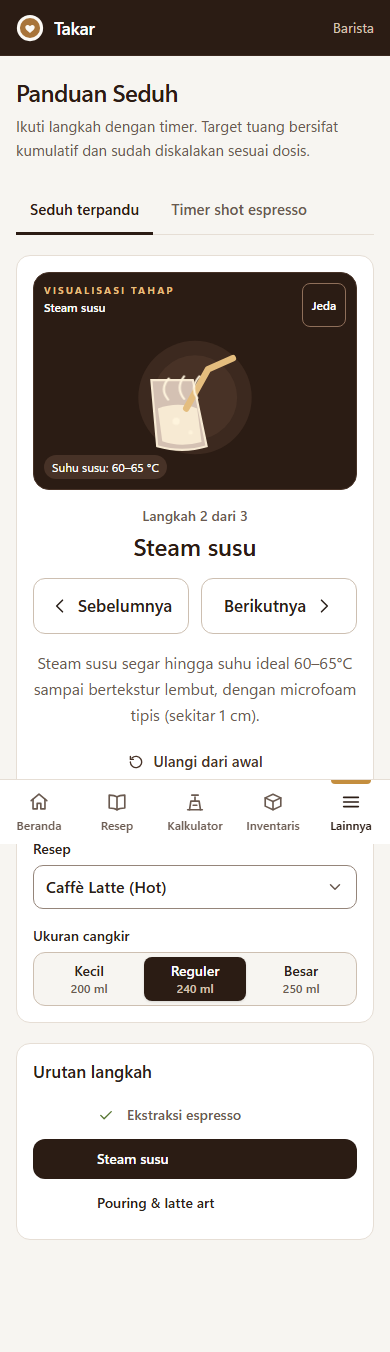
\includegraphics[width=.36\textwidth]{pic/results/screenshots/blackbox/BB-29-pairing-brew-link.png}
\caption{Tahap pengukusan susu Caffè Latte pada ponsel setelah panduan dibuka dari pasangan menu}
\label{fig:lampiran-pairing-mobile}
\end{figure}

\clearpage
\section*{Lampiran G. Contoh Jawaban Asisten dengan Sumber}
\phantomsection
\addcontentsline{toc}{section}{Lampiran G. Contoh Jawaban Asisten dengan Sumber}

Gambar~\ref{fig:lampiran-asisten} memperlihatkan jawaban asisten tentang prosedur V60 dalam BB-27, termasuk langkah dan rujukan yang dapat dibuka. Satu jawaban contoh tidak mewakili seluruh pertanyaan; hasil 60 butir untuk tiap varian dilaporkan pada Bab~\ref{bab:hasil} dan tersimpan di \path{app/results/assistant_eval.json}.

\begin{figure}[htbp]
\centering
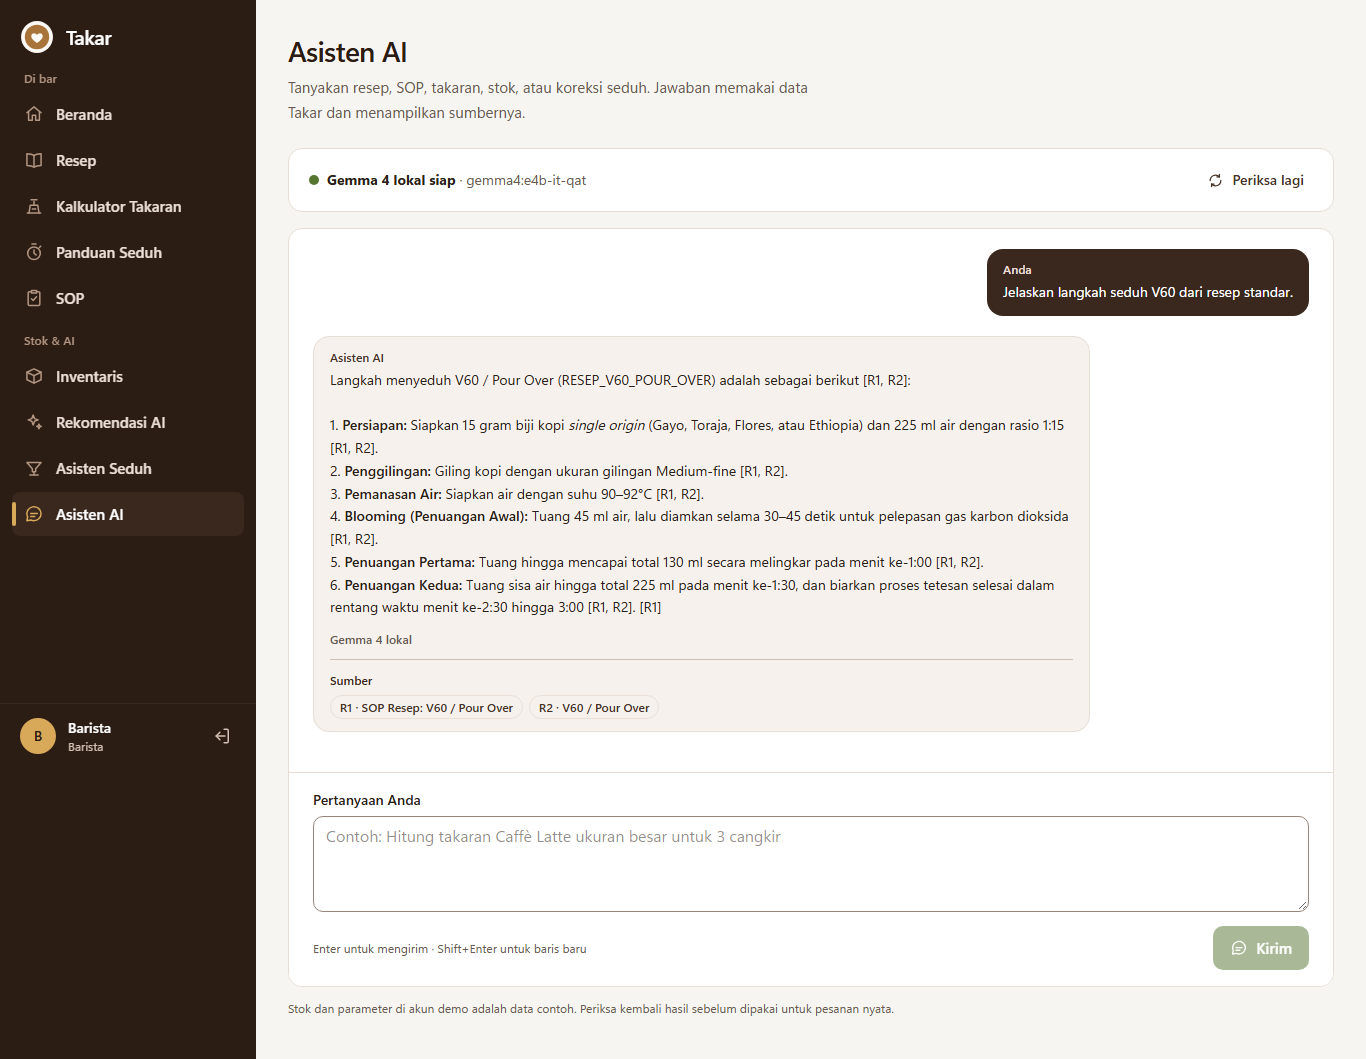
\includegraphics[width=.88\textwidth]{pic/results/screenshots/blackbox/BB-27-assistant-ai.png}
\caption{Jawaban Asisten AI tentang V60 dengan Rujukan Resep dan SOP}
\label{fig:lampiran-asisten}
\end{figure}

% Sampe sini buat lampiran

\end{document}
